\documentclass[11pt]{article}
\usepackage[T1]{fontenc}
\usepackage[utf8]{inputenc}
\usepackage{lmodern}
\usepackage[margin=1in]{geometry}
\usepackage{amsmath,amssymb,amsthm,mathtools}
\usepackage{microtype}
\usepackage{booktabs,array,longtable}
\usepackage{enumitem,needspace}
\usepackage{graphicx,tikz}
\usetikzlibrary{arrows.meta,positioning,calc,fit,decorations.pathreplacing,patterns}
\usepackage{xcolor}
\definecolor{linkblue}{RGB}{22,67,104}
\definecolor{deepblue}{RGB}{35,79,112}
\definecolor{warmred}{RGB}{163,70,55}
\usepackage[colorlinks=true,linkcolor=linkblue,citecolor=linkblue,urlcolor=linkblue,bookmarksnumbered=true]{hyperref}
\hypersetup{
  pdftitle={Rigidity of Smooth Billiards with a Continuous Caustic Collar},
  pdfauthor={OpenAI},
  pdfsubject={Near-boundary Birkhoff conjecture for a continuous physical caustic collar},
  pdfkeywords={convex billiards, Birkhoff conjecture, caustics, rigidity}
}
\usepackage[nameinlink,noabbrev,capitalize]{cleveref}
\numberwithin{equation}{section}
\newtheorem{theorem}{Theorem}[section]
\newtheorem{lemma}[theorem]{Lemma}
\newtheorem{proposition}[theorem]{Proposition}
\newtheorem{corollary}[theorem]{Corollary}
\theoremstyle{definition}
\newtheorem{definition}[theorem]{Definition}
\newtheorem{remark}[theorem]{Remark}
\makeatletter
\newcommand{\TheoremNeedspace}{\if@nobreak\else\Needspace{6\baselineskip}\fi}
\makeatother
\AddToHook{env/theorem/before}{\TheoremNeedspace}
\AddToHook{env/lemma/before}{\TheoremNeedspace}
\AddToHook{env/proposition/before}{\TheoremNeedspace}
\AddToHook{env/corollary/before}{\TheoremNeedspace}
\AddToHook{env/definition/before}{\TheoremNeedspace}
\AddToHook{env/remark/before}{\TheoremNeedspace}
\DeclareMathOperator{\diag}{diag}
\DeclareMathOperator{\dist}{dist}
\DeclareMathOperator{\supp}{supp}
\DeclareMathOperator{\rank}{rank}
\DeclareMathOperator{\ord}{ord}
\DeclareMathOperator{\Res}{Res}
\DeclareMathOperator{\crit}{crit}
\DeclareMathOperator{\Var}{Var}
\DeclareMathOperator{\sgn}{sgn}
\newcommand{\R}{\mathbb R}
\newcommand{\C}{\mathbb C}
\newcommand{\N}{\mathbb N}
\newcommand{\Z}{\mathbb Z}
\newcommand{\Q}{\mathbb Q}
\newcommand{\E}{\mathbb E}
\newcommand{\Prob}{\mathbb P}
\newcommand{\eps}{\varepsilon}
\newcommand{\ind}{\mathbf 1}
\newcommand{\dd}{\,\mathrm d}
\newcommand{\ii}{\mathrm i}
\setlist{topsep=4pt,itemsep=3pt,parsep=0pt}
\setlength{\emergencystretch}{2em}
\title{Rigidity of Smooth Billiards with a Continuous Caustic Collar}
\author{OpenAI}
\date{September 24, 2026}
\begin{document}
\maketitle
\begin{abstract}
We prove that a smooth strictly convex planar billiard with positive
curvature is an ellipse whenever a full neighborhood of its boundary is
continuously foliated by smooth closed convex caustics. No differentiability
across the leaves is assumed. This resolves the near-boundary Birkhoff
conjecture in the stated smooth class.
\end{abstract}
\tableofcontents
\clearpage
\section{Introduction}\label{sec:introduction}
\suppressfloats[t]

The Birkhoff conjecture asks whether an integrable planar convex billiard
must be an ellipse. We prove the version in which integrability is assumed
only in a neighborhood of the boundary, with continuous dependence of the
caustics. The individual leaves and the billiard boundary are smooth;
no differentiability of the foliation across its leaves is required.

\begin{definition}[A continuous caustic collar]\label{def:caustic-collar}
Let \(\Omega\subset\R^2\) be a bounded strictly convex domain whose boundary
is a \(C^\infty\) simple closed regular curve with positive curvature.
A \emph{smooth closed convex caustic} is a \(C^\infty\) simple closed
regular curve in \(\Omega\), bounding a strictly convex set, such that a
billiard segment tangent to the curve remains tangent after reflection
at either endpoint. Here reflection of an incoming unit velocity \(v\)
at a boundary point with outward unit normal \(n\) is
\[
v\longmapsto v-2(v\cdot n)n.
\]
A \emph{continuous caustic collar} consists of a relatively open set
\(A\subset\overline\Omega\) containing \(\partial\Omega\) and a homeomorphism
\[
H_0:\mathbb S^1\times[0,1)\longrightarrow A
\]
such that \(H_0(\mathbb S^1\times\{0\})=\partial\Omega\), and
\(H_0(\mathbb S^1\times\{b\})\) is a smooth closed convex caustic for every
\(0<b<1\).
\end{definition}

\begin{theorem}\label{thm:main}
If \(\Omega\) has a continuous caustic collar, then \(\Omega\) is an ellipse.
Equivalently, there are \(c\in\R^2\) and a real symmetric positive-definite
matrix \(Q\) such that
\[
\Omega=\{x\in\R^2:(x-c)^TQ(x-c)<1\}.
\]
Circles are included.
\end{theorem}

This resolves the near-boundary Birkhoff conjecture positively in the
smooth positively curved class of \Cref{def:caustic-collar}. The collar
contains every intermediate leaf. A Cantor family of invariant curves,
even one accumulating at the boundary, does not satisfy this assumption.
The hypothesis makes no assertion about the billiard dynamics farther
inside the domain.

\begin{figure}[t]
\centering
\begin{minipage}{0.48\textwidth}
\centering
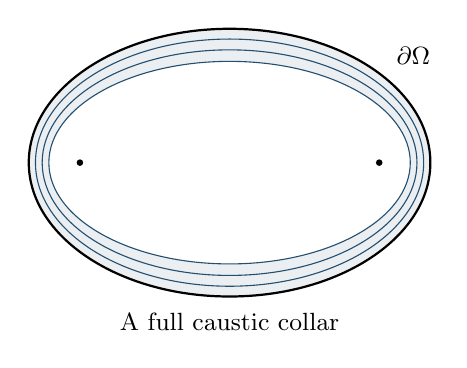
\begin{tikzpicture}[scale=.85,>=Stealth]
\fill[deepblue!9,even odd rule] (0,0) ellipse (3 and 2)
 (0,0) ellipse (2.70 and 1.5133);
\draw[thick] (0,0) ellipse (3 and 2);
\draw[deepblue] (0,0) ellipse (2.90 and 1.8466);
\draw[deepblue] (0,0) ellipse (2.80 and 1.6852);
\draw[deepblue] (0,0) ellipse (2.70 and 1.5133);
\fill (-2.236,0) circle (1.4pt);
\fill (2.236,0) circle (1.4pt);
\node[font=\small] at (0,-2.38) {A full caustic collar};
\node[font=\small,anchor=west] at (2.35,1.6) {$\partial\Omega$};
\end{tikzpicture}
\end{minipage}\hfill
\begin{minipage}{0.48\textwidth}
\centering
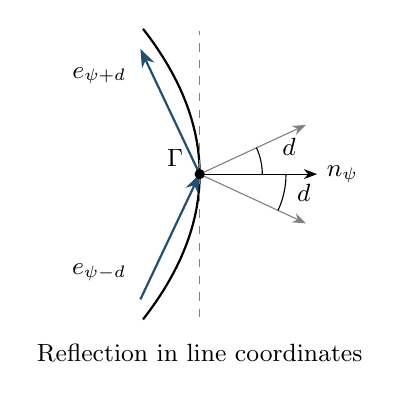
\begin{tikzpicture}[scale=1.42,>=Stealth]
\draw[thick,domain=-1.3:1.3,samples=40,variable=\y]
 plot ({1-.3*\y*\y},{\y});
\draw[dashed,gray] (1,-1.28)--(1,1.28);
\draw[->,deepblue,thick] (.47,-1.12)--(1,0);
\draw[->,deepblue,thick] (1,0)--(.47,1.12);
\draw[->] (1,0)--(2.05,0) node[right,font=\small] {$n_\psi$};
\draw[->,gray] (1,0)--(1.95,-.44);
\draw[->,gray] (1,0)--(1.95,.44);
\draw (1.56,0) arc (0:25:.56);
\draw (1.70,-.326) arc (-25:0:.77);
\node[font=\small] at (1.80,.24) {$d$};
\node[font=\small] at (1.93,-.17) {$d$};
\node[font=\small,anchor=east] at (.43,-.88) {$e_{\psi-d}$};
\node[font=\small,anchor=east] at (.43,.88) {$e_{\psi+d}$};
\fill (1,0) circle (1.3pt);
\node[font=\small,anchor=east] at (.94,.14) {$\Gamma$};
\node[font=\small] at (1,-1.60) {Reflection in line coordinates};
\end{tikzpicture}
\end{minipage}
\caption{The geometric hypothesis and the local reflection convention.
The left panel shows confocal elliptic caustics, the model covered by
the theorem. The shaded collar represents a full family of leaves.
At the impact point \(\Gamma\) in the right panel, \(n_\psi\) is the
outward unit normal. The blue arrows give the incoming and outgoing
unit-velocity directions \(e_{\psi-d}\) and \(e_{\psi+d}\); their line
normals have angles \(\psi-d\) and \(\psi+d\).}
\label{fig:caustic}
\end{figure}


\subsection{History and scope}

Ellipses are the basic integrable examples: their confocal conics supply
caustics, and a confocal elliptic family fills a collar of the boundary.
The conjecture is traditionally attributed to Birkhoff; its early
printed formulation appears in Poritsky's work~\cite{Poritsky1950}.
For the classical dynamical setting and this historical attribution,
see \cite{Birkhoff1927,KS2018}. Poritsky's translation property for
nested string constructions is stronger than the existence of a
foliation~\cite{Poritsky1950}. Lazutkin constructed a positive-measure
family of grazing caustics for sufficiently smooth positively curved
tables~\cite{Lazutkin1973}; its gaps do not give a full collar.
Marvizi and Melrose's interpolating grazing integral is accurate up to
a flat error, rather than an exact integral~\cite{MM1982}. Mather's
obstruction when curvature vanishes underscores the positive-curvature
hypothesis here~\cite{Mather1982}.

Several rigidity theorems establish parts of the conjecture under
additional assumptions. Bialy's rigidity theorem assumes a foliation
of the whole phase cylinder by continuous noncontractible invariant
curves and concludes that the table is a
circle~\cite{Bialy1993}. Innami's theorem concerns convex caustics
whose rotation numbers approach \(1/2\), the opposite endpoint from
grazing rotation zero; Arnold and Bialy give a geometric treatment of
that result~\cite{Innami2002,AB2018}. Bialy and Mironov prove ellipse
rigidity for centrally symmetric tables when the phase annulus reaches
the four-periodic curve, with a corresponding \(C^1\) foliation by
physical caustics through rotation \(1/4\)~\cite{BM2022}. These
hypotheses are not supplied by a small grazing collar.

Perturbative results include the local rigidity work of Avila, De
Simoi and Kaloshin near low-eccentricity ellipses~\cite{ADK2016}, and
Kaloshin and Sorrentino near ellipses of arbitrary
eccentricity~\cite{KS2018}. Kaloshin, Koudjinan and Zhang treat nearly
centrally symmetric domains under specified caustic
conditions~\cite{KKZ2024}; Koval treats small rational-rotation
caustics near almost every ellipse~\cite{Koval2026}. Glutsyuk's
classification for complex algebraic caustics lies in a different
analytic setting~\cite{Glutsyuk2026}.

\Cref{thm:main} assumes none of those perturbative, symmetry, or algebraic
conditions. In particular, we must obtain analytic regularity from the
given smooth geometry and merely continuous foliation. The proof below
does so before using complex continuation. Its grazing normalization
and action expansions have antecedents in Lazutkin and Marvizi--Melrose;
its rational-action Fourier test is related to Avila--De Simoi--Kaloshin;
and its use of complex singularities has a perturbative predecessor in
Kaloshin--Sorrentino~\cite{Lazutkin1973,MM1982,ADK2016,KS2018}.
These are method ancestry, not formal inputs to the arbitrary-table
analytic inversion, first-wall, or probability arguments proved here.

\subsection{The main ideas}

The proof has three parts. First, rational caustics force analytic
regularity. Nesting and area recurrence imply that every sufficiently
small rational rotation occurs on a curve entirely made of periodic
orbits. The actions of these orbits give a high-frequency system whose
derivative is the identity up to a small operator. An analytic Newton
construction then upgrades the boundary from smooth to analytic.
A second construction uses both values and first parameter jets at
rational resonances to obtain a jointly analytic conjugacy at glancing.

Second, finite reflected chains determine their intermediate lines
algebraically from endpoint jets. The proof combines a finite system
for one-variable jets with a coalescing-impact scaling. This local
determination result controls monodromy: a finite first continuation
wall cannot have even one local joint meromorphic patch. The argument
separates finite jet determination from global continuation, and the
corresponding lemmas are stated independently of the later growth
analysis.

Third, we study the complexified boundary through its meromorphic
normal and two analytic derivative fields. Zeros or poles of that
normal force an elliptic form. If there are none, continued impacts
admit one complex shape coordinate. Growth estimates exclude most
possible behaviors at the edge of its strip, leaving a critical
finite-width case. There, moment bounds and paths through regions
where the fields are large limit the total angular change, an
\emph{angle budget}. For one fixed odd periodic chain, matrix identities
transfer that control to Brownian paths stopped before the shape
boundary. Finally, we find a horizontal row on which the first field is
robustly small or large outside a set of vanishing relative measure.
The sign test on this row keeps the last moving impact away from the
boundary, contradicting the assumed first wall.

Two aspects of these arguments may be useful separately. The first is
the finite-chain algebraic determination principle and its monodromy
consequence. The second is the combination of an individual-center
quiet-profile obstruction with moment bounds: a local analytic passage
forces a global width improvement, so even an exceptional sequence of
quiet centers is ruled out. The subsequent probability arguments use
this pointwise conclusion explicitly.

\Needspace{20\baselineskip}
\subsection{Organization and dependencies}

The sections and their main deductions are recorded below. The
arbitrary-input action estimates of \Cref{ana:section} are separate from
the geometric vanishing supplied by the caustic collar. The parameter
jets in \Cref{joint:section} use the full collar again.

\begin{center}
\begin{tabular}{@{}p{0.24\textwidth}p{0.69\textwidth}@{}}
\toprule
Location & Role in the proof \\
\midrule
\Cref{ana:section,joint:section}
& Rational-action inversion gives an analytic boundary; rational jets give a jointly analytic glancing parametrization. \\
\Cref{sec:continuation}
& Finite-chain algebraic determination rules out a local patch at a first continuation wall. \\
\Cref{sec:shapes}
& Zeros or poles of the normal force an ellipse; otherwise impacts lift to a global shape coordinate. \\
\Cref{sec:cones,sec:profiles}
& Kernel continuation and profile obstructions reduce growth to a critical finite wall. \\
\Cref{sec:critical,sec:model}
& Conditional critical estimates precede the independent exclusion of prohibited sequences; only then is the angle budget activated. \\
\Cref{sec:odd-slice,sign:section}
& Stopped odd-chain geometry and a sign row exclude the critical wall and complete \Cref{thm:main}. \\
\bottomrule
\end{tabular}
\end{center}

There is one deliberate forward reference: the angle-budget reduction
uses the exclusion of a precisely stated class of sequences, proved in
the following section. That exclusion uses the earlier moment and
continuation estimates, not the angle budget. The final proof of
\Cref{thm:main} assembles the alternatives after \Cref{thm:last-site}.

\subsection{Conventions}

Angles are real lifts of \(2\pi\)-periodic variables. Complex Euclidean
products are bilinear, without complex conjugation. A meromorphic
projective map means meromorphic affine coordinates in a generic chart;
all incidence identities are used on their regular locus and then
continued. Constants denoted by \(C\) may increase between estimates.
Dependence on a fixed aperture or another fixed auxiliary parameter is
displayed when it matters for an order of choices.

The normalized generating action is denoted by \(D\). Later, an uppercase
\(D\) also denotes a positive rescaled depth inside a local scaling
argument; its meaning is stated there. To keep the width bookkeeping
distinct, the phase-width deficit is denoted throughout by
\(\Delta(t)=H-h_X(t)\). Horizontal expectations are normalized averages
over one period unless a different probability law is specified.

\section{Rational caustics and analytic regularity}\label{ana:section}

The first task is to obtain analytic regularity from the continuous
foliation in \Cref{def:caustic-collar}.  The argument uses only the rational
leaves with rotation number \(1/q\).  Their critical actions define a system
of equations whose derivative on sufficiently high Fourier modes is close
to the identity.  The small loss of complex width in the construction of
each individual equation is compatible with an inverse on a single
exponentially weighted Fourier space.
The coordinate follows Lazutkin's grazing normalization, and the
action viewpoint is related to Marvizi--Melrose's asymptotic
interpolation~\cite{Lazutkin1973,MM1982}. Rational-caustic Fourier
constraints also appear in the perturbative work of Avila, De Simoi
and Kaloshin~\cite{ADK2016}. The arbitrary-input mesh, Fourier row,
and nonperturbative inversion required here are proved below.

\begin{theorem}[Analytic regularity]\label{thm:analytic}
Under the hypotheses of \Cref{thm:main}, the support function of the table
and its boundary are real analytic.
\end{theorem}

\subsection{The invariant graphs and their rational leaves}

Classical invariant-graph results for twist maps give context for this
phase description~\cite{Arnaud2009}; periodic billiard graphs are also
studied in \cite[Appendix~A]{FS2026}. The all-point rational periodicity
needed here follows directly from the filled collar in the next lemma.

Translate an interior point to the origin.  Write
\[
n_\theta=(\cos\theta,\sin\theta),\qquad
e_\theta=(-\sin\theta,\cos\theta).
\]
The support function \(h\) is smooth, and the point with outward normal
\(n_\psi\) is
\[
\gamma(\psi)=h(\psi)n_\psi+h'(\psi)e_\psi.
\]
The curvature assumption gives
\[
r(\psi)=h(\psi)+h''(\psi)>0.
\]
All angles below are real lifts of variables of period \(2\pi\).
An oriented line near a positively oriented supporting line is described
by its velocity \(e_\theta\) and its equation \(n_\theta\cdot x=p\).
If its forward reflection has outgoing angle \(\theta'\), put
\(\psi=(\theta+\theta')/2\) and \(d=(\theta'-\theta)/2\).  On the small
positive branch, the reflection law gives
\[
\begin{split}
\theta&=\psi-d,\qquad \theta'=\psi+d,\\
p&=h(\psi)\cos d-h'(\psi)\sin d,\\
p'&=h(\psi)\cos d+h'(\psi)\sin d.
\end{split}
\]
The billiard map has Bialy and Mironov's support-function generating
action~\cite{BM2017}:
\begin{equation}\label{ana:line-generating-function}
\mathcal S(\theta,\theta')
=2h\left(\frac{\theta+\theta'}2\right)
 \sin\left(\frac{\theta'-\theta}2\right),
\qquad
p=-\mathcal S_1,\quad p'=\mathcal S_2.
\end{equation}
In particular,
\begin{equation}\label{ana:twist}
\mathcal S_{12}(\theta,\theta')
=\frac{r(\psi)}2\sin d>0.
\end{equation}
This map preserves \(\dd p\wedge\dd\theta\), and
\(\partial\theta'/\partial p=-1/\mathcal S_{12}<0\).

\begin{lemma}\label{lem:rational-periodicity}
There is a one-sided phase collar filled by invariant continuous graphs
\(p=g_b(\theta)\), where \(b>0\) increases towards the interior and
\(g_b\) strictly decreases pointwise.  The induced increasing lifts
\(F_b\) have positive translation numbers \(\tau(b)\), tending to zero
as \(b\downarrow0\).

For every sufficiently small positive rational number \(l/q\), in lowest
terms, there is exactly one graph with
\(\tau(b)=2\pi l/q\), and its lift satisfies
\begin{equation}\label{ana:rational-identity}
F_b^q(\theta)=\theta+2\pi l
\qquad\text{for every }\theta.
\end{equation}
\end{lemma}

\begin{proof}
Restrict the foliation parameter to a compact interval close to zero.
Continuity of its parametrizing homeomorphism gives uniform convergence
of the leaf curves to the outer boundary.  Support functions are
continuous for this convergence.  Hence the convex bodies bounded by
the leaves contain the origin for sufficiently small parameters.
Two disjoint convex boundary curves surrounding the origin are nested:
otherwise their radial functions change order and the curves intersect.
Their compact disjointness makes the nesting strict, including strict
ordering of their support functions in every direction.  It follows,
using the limiting outer boundary, that \(g_b(\theta)\) is continuous
and strictly decreasing in \(b\), for each \(\theta\).
The intervals it fills, as \(\theta\) varies, form a phase collar.

Every positively oriented supporting line of a leaf in this collar
reflects to another positively oriented supporting line of the same
leaf.  Indeed the reflected line is tangent by the caustic property.
For a sufficiently small collar both the incoming and outgoing lines
are close to the corresponding positive outer supporting lines.
The other orientation of a leaf support has coordinate
\(-g_b(\theta+\pi)\), which stays negative because the bodies contain
a fixed neighborhood of the origin.  Thus this orientation cannot
occur.  The same argument applies to the inverse reflection.
The billiard map therefore restricts to a circle homeomorphism of each
graph.  It is close to the identity and consequently has degree one.
Its lift \(F_b\) is increasing, has strictly positive increments, and
depends continuously on \(b\).  By \Cref{ana:twist}, these lifts are
strictly ordered as \(b\) increases.

We recall the elementary rotation facts needed here.  For an increasing
lift \(F\) commuting with translation by \(2\pi\), the oscillation of
\(F^m(x)-x\) is at most \(2\pi\).  The maximum and minimum of this
displacement are respectively subadditive and superadditive in \(m\).
It follows that
\[
\tau(F)=\lim_{m\to\infty}\frac{F^m(x)-x}{m}
\]
exists, is independent of \(x\), and satisfies
\[
\left|\tau(F)-\frac{F^m(x)-x}{m}\right|\le\frac{2\pi}{m}.
\]
This bound gives continuity of \(\tau\) under uniform convergence of
lifts.  Ordering lifts orders their iterates and hence their translation
numbers.  A lift with translation number zero has a fixed point: if its
displacement never vanishes, its sign is constant and its absolute value
has a positive minimum.  Applied to \(F^q-2\pi l\), this says that
\(\tau(F)=2\pi l/q\) implies the existence of a \(q\)-periodic point.
Conversely, such a point forces that translation number.

These facts show that \(\tau(b)\) is continuous and nondecreasing.
Its positivity follows from the positive minimum of \(F_b(\theta)-\theta\)
on each fixed graph; its limit at zero follows from uniform convergence
of the map to the identity.

There cannot be a nontrivial interval of parameters with the same
rational translation number \(2\pi l/q\).  Otherwise the closed annulus
between two distinct graphs in that interval is invariant and has
positive finite area.  Almost every point in it is recurrent for the
\(q\)-th iterate, by finite-measure recurrence.  On a graph of the
specified rotation number, \(F_b^q-2\pi l\) has fixed points.  Every
point in a component of their complement moves strictly monotonically
towards an endpoint of that component and is not recurrent.
Thus the \(q\)-th iterate is the identity almost everywhere in the
annulus, and hence everywhere by continuity.  This contradicts strict
ordering of the \(q\)-th iterates on its two boundary graphs.

Continuity now supplies a unique graph at each sufficiently small
positive rational rotation, with smaller and larger rotations
arbitrarily close on its two sides.  A lift with rotation greater than
\(2\pi l/q\) has \(F^q(\theta)-\theta-2\pi l>0\) everywhere: a zero
would force that rational rotation, and a strictly negative displacement
would force a smaller one.  The corresponding inequality is reversed
below that rotation.  Passing to the graph in question proves
\Cref{ana:rational-identity}.
\end{proof}

\subsection{The normalized action}

Choose \(k>0\) so that the coordinate defined by
\[
\frac{\dd x}{\dd\theta}=k r(\theta)^{1/3}
\]
has period \(2\pi\).  Write \(\theta=\phi(x)\), and set
\begin{equation}\label{ana:normalization}
\phi'(x)=e^{u(x)},\qquad
r(\phi(x))=c e^{-3u(x)},\qquad c=k^{-3}.
\end{equation}
For the table, \(u\) is real, smooth, and periodic.  Subtract
\(\int_\theta^{\theta'}h(\eta)\,\dd\eta\) from \(\mathcal S\), change
coordinates, and divide by \(c\).  The subtracted term telescopes in
every fixed-endpoint action, so these operations preserve stationarity.
Integration by parts using \(h+h''=r\) gives the resulting action:
\begin{equation}\label{ana:normalized-action}
\begin{split}
D(X,Y)={}&-\int_X^\mu
 \bigl(1-\cos(\phi(z)-\phi(X))\bigr)e^{-2u(z)}\,\dd z\\
&-\int_\mu^Y
 \bigl(1-\cos(\phi(Y)-\phi(z))\bigr)e^{-2u(z)}\,\dd z,
\qquad
\phi(\mu)=\frac{\phi(X)+\phi(Y)}2 .
\end{split}
\end{equation}
For clarity, before the coordinate change the corresponding two
integrands are \(r(\eta)(1-\cos(\eta-\theta))\) and
\(r(\eta)(1-\cos(\theta'-\eta))\), respectively.  Substitution of
\(r(\phi(z))\phi'(z)/c=e^{-2u(z)}\) gives
\Cref{ana:normalized-action}.

The following action formula and mesh estimates apply to arbitrary
input; the caustic hypothesis is used separately to make the resulting
constraints vanish. We will use this formula for arbitrary real smooth
periodic \(u\).
In that case let \(\phi\) be any primitive of \(e^u\).  Its total
increment need not be \(2\pi\): all occurrences of \(\phi\) are
differences, so \(D\) remains diagonally \(2\pi\)-periodic.  For small
\(Y-X\), the midpoint is uniquely defined.  The formula also gives
\begin{equation}\label{ana:action-symmetries}
D(X+2\pi,Y+2\pi)=D(X,Y),\qquad D(Y,X)=-D(X,Y).
\end{equation}
If \(u\) is holomorphic in a strip, these definitions are holomorphic
near its diagonal.  All small complex integrals may be taken along
straight segments.

Differentiating the two integrals in \Cref{ana:normalized-action}, the
moving-midpoint terms cancel.  Thus
\begin{equation}\label{ana:D1-integral}
D_1(X,X+T)=
e^{u(X)}\int_X^\mu
\sin(\phi(z)-\phi(X))e^{-2u(z)}\,\dd z.
\end{equation}
The following expansion will also fix the normalization used in the
next Section:
\begin{equation}\label{ana:action-expansion}
\begin{split}
D_1(X,X+T)&=\frac{T^2}{8}+a(X)T^4+O(T^5),\\
a(X)&=\frac{7u''(X)-8u'(X)^2-e^{2u(X)}}{384},\\
D(X,X+T)&=-\frac{T^3}{24}-\frac{a(X)}5T^5+O(T^6).
\end{split}
\end{equation}
Here and below the remainders have the differentiated bounds specified
in the lemmas where they are used.  One direct calculation is as
follows.  Put \(\alpha=u'(X)\), \(\beta=u''(X)\), \(A=e^{u(X)}\), and
\(z=(\mu-X)/T\).  The midpoint equation gives
\[
z=\frac12+\frac{\alpha T}{8}+\frac{\beta T^2}{16}+O(T^3).
\]
After rescaling \Cref{ana:D1-integral}, its integrand is
\[
v-\frac32\alpha T v^2
+\frac{7\alpha^2-5\beta-A^2}{6}T^2v^3+O(T^3).
\]
Integrating to \(z\) gives the first two lines of
\Cref{ana:action-expansion}; in particular its linear term in \(T\)
vanishes.  The leading term of \(D\) follows directly from its integral.
Antisymmetry forces its fourth-order coefficient to vanish.
Finally, if \(d_5(X)\) is its fifth-order coefficient, differentiation
with respect to the first endpoint at fixed second endpoint gives
\(-5d_5=a\), proving the last line.

\subsection{Uniform stationary meshes}

For \(\sigma>0\) let
\[
\mathcal A_\sigma=\{z\in\C:|\Im z|<\sigma\},\qquad
\|f\|_{a,\sigma}=\max_{0\le j\le a}
                  \sup_{\mathcal A_\sigma}|f^{(j)}|.
\]
Functions in a positive strip are holomorphic and periodic; they are
real symmetric if \(f(\bar z)=\overline{f(z)}\).
For \(\sigma=0\), the same norm means the \(C^a\) norm on the real
circle.  Constants in the lemmas below do not depend on \(\sigma\).

\begin{lemma}\label{ana:mesh-lemma}
Fix an integer \(m\ge2\), a bound \(M\), and put
\(p=m+2\), \(r_0=m+15\).
There are \(R,K,N\), depending only on \(M,m\), with the following
properties.  Suppose \(0\le\sigma\le1\), \(u\) is real symmetric, and
\(\|u\|_{r_0,\sigma}\le M\).  For every integer \(q\ge N\), let
\(\delta=2\pi/q\).  There is a stationary fixed-endpoint mesh
\begin{equation}\label{ana:mesh-definition}
X_j(x)=x+j\delta+w_j(x),\qquad 0\le j\le q,\qquad
w_0=w_q=0,
\end{equation}
on \(\mathcal A_{\sigma'}\), where
\(\sigma'=(1-K/q^2)\sigma\), satisfying
\begin{equation}\label{ana:mesh-norm}
\|w\|_*:=
q^2\max_j\|w_j\|_{p,\sigma'}
+q^3\max_j\|w_{j+1}-w_j\|_{p,\sigma'}\le R.
\end{equation}
It depends differentiably on smooth real variations of \(u\), and
\[
\|\dot w\|_*\le C\|\dot u\|_{r_0,\sigma}.
\]
The analogous difference estimate holds for two inputs in this ball.
On the real axis, the mesh is also unique pointwise in the ball with
the same scaled position and step bounds.  This real uniqueness ball
may be enlarged by any fixed amount if \(N\) is increased.
\end{lemma}

\begin{proof}
We give the composition estimates, including their width dependence.
For a trial mesh in the ball \Cref{ana:mesh-norm}, set
\[
X=X_j,\qquad s=X_j-X_{j-1},\qquad t=X_{j+1}-X_j.
\]
Then \(s,t=\delta+O(q^{-3})\) in \(C^p\).
For \(T=t\) or \(T=-s\), and \(0\le\lambda\le1\), write
\(\mu=X+\lambda T z_\lambda\).  The midpoint equation is
\begin{equation}\label{ana:midpoint-equation}
\int_0^{z_\lambda}
 e^{u(X+\lambda Tv)-u(X)}\,\dd v
=\frac12\int_0^1e^{u(X+\lambda Tv)-u(X)}\,\dd v .
\end{equation}
Moving the integrals of the exponential minus one to the other side
expresses \(z_\lambda-1/2\) as a contraction on a \(C^p\) ball of
radius \(C/q\).  Indeed the exponential minus one is \(O(q^{-1})\);
its derivative with respect to \(z_\lambda\), after writing the
left integral as an integral over \(v=\alpha z_\lambda\), has the
same bound.  Products and compositions in this argument are estimated
by the ordinary finite-order chain rule.

All its evaluation points lie in the original strip.  Their maps from
\(x\) are real symmetric and have derivative \(1+O(q^{-2})\):
\[
X'=1+O(q^{-2}),\qquad T'=O(q^{-3}),\qquad
z_\lambda'=O(q^{-1}).
\]
For a real-symmetric map \(x+\rho+e(x)\), with \(\rho\) real and
\(\|e'\|\le Cq^{-2}\), integration along the vertical segment from
\(\Re x\) gives
\[
|\Im(x+\rho+e(x))|\le(1+Cq^{-2})|\Im x|.
\]
Taking \(K\) sufficiently large therefore puts every such point,
and every segment used in the integrals, inside \(\mathcal A_\sigma\).
This is a relative loss \(K\sigma/q^2\), with no reciprocal power of
\(\sigma\).

Implicit differentiation of \Cref{ana:midpoint-equation} gives, for
\(1\le i\le3\),
\begin{equation}\label{ana:midpoint-jets}
\|\partial_\lambda^i z_\lambda\|_{p,\sigma'}\le Cq^{-i}.
\end{equation}
To see the scaling, the coefficient of the derivative being solved
for is \(e^{u(X+\lambda Tz_\lambda)-u(X)}=1+O(q^{-1})\).
Each explicit \(\lambda\)-derivative contributes a factor \(T\);
the lower implicit derivatives satisfy the same induction.
For a mesh variation,
\[
\|\dot X\|_{p,\sigma'}\le q^{-2}\|\dot w\|_*,
\qquad
\|\dot T\|_{p,\sigma'}\le q^{-3}\|\dot w\|_*.
\]
Differentiating the same equations therefore gives, for \(1\le i\le3\),
\begin{equation}\label{ana:midpoint-variation}
\|\partial_\lambda^i\dot z_\lambda\|_{p,\sigma'}
\le Cq^{-i}
 \bigl(q^{-2}\|\dot w\|_*+\|\dot u\|_{r_0,\sigma}\bigr).
\end{equation}
For \(i=0\) the right hand side has an additional factor \(q^{-1}\).
For example, a difference \(u(B)-u(X)\) is written as the integral
of \(u'\) from \(X\) to \(B\).  Its variation in a changed basepoint
uses a difference of \(u'\), hence retains the factor \(B-X=O(q^{-1})\).
This proves the extra factor also for variations, rather than merely
for the values.

The rescaled expression for \Cref{ana:D1-integral} is
\[
\begin{split}
F(\lambda)
&=(\lambda T)^{-2}D_1(X,X+\lambda T)\\
&=e^{u(X)}\int_0^{z_\lambda}
\frac{\sin\left(\lambda T\int_0^v
                 e^{u(X+\lambda Tv')}\,\dd v'\right)}{\lambda T}
 e^{-2u(X+\lambda Tv)}\,\dd v .
\end{split}
\]
The quotient at zero is removable: write it as
\(A_\lambda(v)\operatorname{sinc}(\lambda T A_\lambda(v))\), where
\(A_\lambda(v)=\int_0^v e^{u(X+\lambda Tv')}\,\dd v'\) and
\(\operatorname{sinc}z=\sin z/z\).
Thus \Cref{ana:midpoint-jets,ana:midpoint-variation} apply to this
expression and its first variations.  The calculation following
\Cref{ana:action-expansion} gives
\[
F(0)=\frac18,\qquad F'(0)=0,\qquad F''(0)=2a(X)T^2.
\]
More explicitly, its third derivative has \(C^p\) norm at most
\(Cq^{-3}\), and the third derivative of its first variation has
norm at most
\[
Cq^{-3}\bigl(q^{-2}\|\dot w\|_*+\|\dot u\|_{r_0,\sigma}\bigr).
\]
Taylor's integral remainder gives
\begin{equation}\label{ana:D1-uniform-expansion}
D_1(X,X+T)
=T^2\left(\frac18+a(X)T^2+T^3b(X,T)\right),
\end{equation}
where the evaluated functions \(a(X)\), \(b(X,T)\) have bounded
\(C^p\) norms.  Their first variations are bounded by
\[
C\bigl(q^{-2}\|\dot w\|_*+\|\dot u\|_{r_0,\sigma}\bigr).
\]
In dividing the Taylor remainder by \(T^3\), no small denominator
is lost: \(qT\) is \(C^p\)-close to \(2\pi\) or \(-2\pi\), while
\(\dot T/T=O(q^{-2}\|\dot w\|_*)\).

We record a finite derivative budget for these statements.  Third
\(\lambda\)-derivatives of the midpoint and integrand use derivatives
of \(u\) through order \(p+3\); their first variations use order \(p+4\).
The estimates for differences follow from
\[
f\circ A-f\circ B
=\int_0^1 f'(B+\alpha(A-B))(A-B)\,\dd\alpha
\]
and the \(C^p\) chain rule, with the straight segment inside the
input strip.  Allowing two further derivatives covers all the
coefficient and composition bounds just used.  Thus \(p+6\)
derivatives already suffice here, fewer than \(r_0=p+13\).
There has been no Cauchy estimate on \(u\), so these constants are
uniform also as \(\sigma\downarrow0\).

Antisymmetry of \(D\) makes the Euler equation at \(X_j\)
\[
D_1(X,X+t)-D_1(X,X-s)=0.
\]
Using \Cref{ana:D1-uniform-expansion} and factoring \(t^2-s^2\)
rewrites it as
\begin{equation}\label{ana:mesh-fixed-point}
w_{j+1}-2w_j+w_{j-1}
=-\frac{t^5b(X,t)+s^5b(X,-s)}
 {(t+s)\bigl(1/8+(t^2+s^2)a(X)\bigr)}.
\end{equation}
The right hand side is \(O(q^{-4})\) in \(C^p\), and its Lipschitz
constant in the starred mesh norm is \(O(q^{-6})\).
For example its numerator is \(O(q^{-5})\), its denominator has
size comparable to \(q^{-1}\), and a unit starred variation changes
each coefficient and each relative step by \(O(q^{-2})\).
These statements hold for complex values as well, since the
denominator is uniformly separated from zero.

The Dirichlet inverse of the second difference has norm at most
\(Cq^4\) from uniform \(C^p\) forcing into the starred norm.
Indeed, if the forcing is \(f_j\), set \(d_j=w_j-w_{j-1}\).
Then
\[
d_{j+1}=d_j+f_j,\qquad
d_1=-\frac1q\sum_{i=1}^{q-1}(q-i)f_i.
\]
It follows that \(\max\|d_j\|_{C^p}\le Cq\max\|f_j\|_{C^p}\)
and \(\max\|w_j\|_{C^p}\le Cq^2\max\|f_j\|_{C^p}\).
Equation \eqref{ana:mesh-fixed-point} is consequently a contraction
with constant \(Cq^{-2}\).  Choose \(R\) larger than its uniform
image bound, then choose the width constant and \(N\).
The image bound can be taken independently of this fixed \(R\):
once \(q\) is large depending on \(R\), all scaled steps and
derivatives in the preceding estimates lie in fixed bounded sets.

Differentiating the contraction gives the asserted input derivative
bound; comparing its fixed points gives the corresponding Lipschitz
bound.  The same argument with order-zero real norms proves pointwise
uniqueness and works in any larger fixed real ball after increasing
\(N\).  It follows in particular that constructions made with different
fixed smoothness bounds or widths agree on their real domains for all
sufficiently large \(q\).
\end{proof}

\subsection{The high-frequency equations}

For the mesh in \Cref{ana:mesh-lemma}, define its critical action and
two associated Fourier coefficients by
\begin{equation}\label{ana:constraint-definition}
W_q(x;u)=\sum_{j=0}^{q-1}D(X_j(x),X_{j+1}(x)),\qquad
C_n(u)=-\frac{q^2}{6\pi}[W_q(\,\cdot\,;u)]_n,\quad n=\pm q,
\end{equation}
where
\[
[f]_n=\frac1{2\pi}\int_0^{2\pi}e^{-\ii nx}f(x)\,\dd x.
\]
Real pointwise uniqueness makes these definitions compatible when
the construction is performed on different strips or with different
fixed smoothness bounds.

\begin{proposition}\label{prop:high-frequency-estimate}
For each integer \(m\ge2\) and \(M<\infty\), take \(r_0=m+15\).
There are constants \(K,N\), independent of \(0\le\sigma\le1\),
such that, whenever \(\|u\|_{r_0,\sigma}\le M\) and \(|n|\ge N\),
the derivative of \Cref{ana:constraint-definition} has the form
\begin{equation}\label{ana:constraint-derivative}
(\dd C_n)_u(v)=[b_n(u)v]_n.
\end{equation}
Here
\begin{equation}\label{ana:coefficient-estimate}
\|b_n(u)-1\|_{m,(1-K/n^2)\sigma}\le\frac{K}{|n|},
\end{equation}
and, for two such inputs on the same strip,
\begin{equation}\label{ana:coefficient-lipschitz}
\|b_n(u)-b_n(\widetilde u)\|_{m,(1-K/n^2)\sigma}
\le\frac{K}{|n|}\|u-\widetilde u\|_{r_0,\sigma}.
\end{equation}
The derivative identity holds for smooth real variations, and for
real-symmetric holomorphic variations with the indicated finite norms.
\end{proposition}

\begin{proof}
Put \(q=|n|\) and \(p=m+2\).  In varying the critical action, all interior
mesh-variation terms vanish by stationarity.  The endpoints \(x\)
and \(x+2\pi\) are fixed.  We may therefore keep the vertices fixed
and differentiate \(D\) directly with respect to \(u\).

On the left half of a cell \((X,X+t)\), differentiation of
\Cref{ana:normalized-action} and reversal of the two integrations give
the kernel
\begin{equation}\label{ana:variation-kernel}
\begin{split}
\mathcal K_-(z)={}&
2\bigl(1-\cos(\phi(z)-\phi(X))\bigr)e^{-2u(z)}\\
&-e^{u(z)}
\int_z^\mu\sin(\phi(\zeta)-\phi(X))e^{-2u(\zeta)}\,\dd\zeta ,
\end{split}
\end{equation}
integrated against \(v(z)\,\dd z\).
On the right half, the corresponding formula is
\[
\begin{split}
\mathcal K_+(z)={}&
2\bigl(1-\cos(\phi(X+t)-\phi(z))\bigr)e^{-2u(z)}\\
&-e^{u(z)}
\int_\mu^z\sin(\phi(X+t)-\phi(\zeta))
                  e^{-2u(\zeta)}\,\dd\zeta .
\end{split}
\]
The moving-midpoint terms cancel because the two original integrands
agree at \(\mu\).

Parametrize the two halves, always from left to right, by
\[
z_-(x,\alpha)=X+\alpha(\mu-X),\qquad
z_+(x,\alpha)=\mu+\alpha(X+t-\mu),\qquad 0\le\alpha\le1,
\]
and set
\(\tau_-=\alpha/2\), \(\tau_+=(1+\alpha)/2\).
Uniformly in \(j,\alpha\), the mesh and midpoint estimates give
\begin{equation}\label{ana:half-cell-estimates}
\begin{split}
z_\pm(x,\alpha)
 &=x+(j+\tau_\pm)\delta+O_{C^p}(q^{-2}),\\
(z_\pm)_\alpha&=\frac{\pi}{q}+O_{C^p}(q^{-2}),\\
\mathcal K_\pm(z_\pm(x,\alpha))
 &=q^{-2}k_0(2\pi\tau_\pm)+O_{C^p}(q^{-3}),
\end{split}
\end{equation}
where
\begin{equation}\label{ana:leading-kernel}
k_0(\xi)=\frac32\min(\xi,2\pi-\xi)^2-\frac{\pi^2}{2},
\qquad 0\le\xi\le2\pi.
\end{equation}
Each remainder in \Cref{ana:half-cell-estimates} has the corresponding
Lipschitz bound, with the same power of \(q\), in
\(\|u-\widetilde u\|_{r_0,\sigma}\).

Here is a verification of both the leading terms and the remainder
orders.  On a cell, replace each occurrence of \(u\) by its value at
\(X\), using the integrated identity for differences of \(u\).
Then replace \(\sin a\) by \(a\) and \(1-\cos a\) by \(a^2/2\);
every phase difference is \(O(q^{-1})\).  On the left this gives
\[
\mathcal K_-(z)
=(z-X)^2-\int_z^\mu(\zeta-X)\,\dd\zeta+O_{C^p}(q^{-3})
=\frac32(z-X)^2-\frac12(\mu-X)^2+O_{C^p}(q^{-3}).
\]
The constant exponential factors cancel.  The reflected expression
gives the right half.  Since
\[
z-X=\delta\tau_-+O_{C^p}(q^{-2}),\qquad
\mu-X=\delta/2+O_{C^p}(q^{-2}),
\]
and similarly from the right endpoint, these formulas give
\Cref{ana:leading-kernel}.  An integrated difference gains one
factor \(q^{-1}\) also after \(p\) derivatives.  Applying the
composition-difference identity used in \Cref{ana:mesh-lemma} proves
the same gain for input variations.  For completeness, the mesh
coefficient estimates used at most \(p+6\) input derivatives; one
further derivative for an integrated spatial difference and one for
its moving-point variation bound all the kernel estimates by
\(C^{p+8}=C^{m+10}\) input norms.  This is still below \(r_0\).

For each \(j,\alpha\) and sign, the real map \(x\mapsto z_\pm(x,\alpha)\)
is an increasing lift close to a real translation.  Write its inverse
as \(x=x_\pm(z,\alpha)\).
On a strip \(\mathcal A_{\sigma''}\), with
\(\sigma''=(1-K/q^2)\sigma\) and a larger \(K\), it satisfies
\begin{equation}\label{ana:inverse-half-cell}
x_\pm(z,\alpha)
=z-(j+\tau_\pm)\delta+O_{C^{m+1}}(q^{-2}).
\end{equation}
This estimate and its Lipschitz version use no additional input
derivatives.  In fact the forward error is \(O(q^{-2})\) in
\(C^{m+2}\).  Its inverse equation is a contraction in \(C^{m+1}\),
since a composition difference there uses just one additional
derivative of the forward error.  Real symmetry gives exactly the
relative imaginary displacement used in the mesh construction, so a
larger relative strip loss suffices for this inverse as well.

Change the Fourier integration variable from \(x\) to \(z\).
The integration interval may start at a different point, but its
length is \(2\pi\), and all integrands are periodic.  Formula
\eqref{ana:constraint-derivative} follows with
\begin{equation}\label{ana:bn-formula}
b_n(z)=
-\frac{q^2}{6\pi}
\sum_{j=0}^{q-1}\sum_{\pm}
\int_0^1
\mathcal K_\pm(z)\,
(z_\pm)_\alpha(x_\pm(z,\alpha),\alpha)\,
(x_\pm)_z(z,\alpha)\,
e^{-\ii n(x_\pm(z,\alpha)-z)}\,\dd\alpha .
\end{equation}
In this formula the kernel is that of the cell belonging to the
indicated \(j,\alpha,\pm\), evaluated after the inverse substitution.

The phase in \Cref{ana:bn-formula} has leading value
\[
e^{\ii n(j+\tau_\pm)\delta}
=e^{2\pi\ii\sgn(n)\tau_\pm}.
\]
Its error, and the error in each of its first \(m\) derivatives,
is \(O(q^{-1})\), since \(|n|=q\) multiplies the
\(O_{C^{m+1}}(q^{-2})\) inverse displacement.
The same statement holds for input differences.
Substituting the leading terms in \Cref{ana:bn-formula} thus gives
\[
-\frac13\int_0^1 k_0(2\pi\tau)e^{2\pi\ii\sgn(n)\tau}\,\dd\tau .
\]
The integral equals \(-3\).  Indeed symmetry reduces it to
\[
\frac1\pi\int_0^\pi
\left(\frac32\xi^2-\frac{\pi^2}{2}\right)\cos\xi\,\dd\xi=-3.
\]
The leading coefficient is therefore \(1\).

Each cell contributes \(O(q^{-1})\) to the leading coefficient and
\(O(q^{-2})\) to its error: the kernel, prefactor, and cell Jacobian
have respective sizes \(q^{-2},q^2,q^{-1}\), and their errors have
one further factor \(q^{-1}\). These are absolute estimates, including
at zeros of the leading kernel \(k_0\). Summation over \(q\) cells proves
\Cref{ana:coefficient-estimate}.  Since the leading term is independent
of \(u\), the same computation with differences proves
\Cref{ana:coefficient-lipschitz}.  The finite derivative budgets above
and the relative domain losses prove the stated uniformity in
\(\sigma\), including \(\sigma=0\).
\end{proof}

\begin{lemma}\label{ana:real-periodic-mesh}
For the function \(u\) associated with the actual table by
\Cref{ana:normalization},
\begin{equation}\label{ana:constraint-vanishing}
C_n(u)=0
\qquad\text{for all sufficiently large }|n|.
\end{equation}
\end{lemma}

\begin{proof}
The rational graphs of rotation \(2\pi/q\) tend to the boundary:
otherwise their parameters have a positive subsequential lower bound,
whereas every fixed positive leaf has positive rotation.
By \Cref{lem:rational-periodicity}, the successive \(x\)-coordinates
on each such graph form a positive stationary mesh of \(q\) steps
whose sum is \(2\pi\).  All its steps tend uniformly to zero.

Let \(s,t\) be consecutive steps.  The real Taylor expansion
\eqref{ana:D1-uniform-expansion} first gives \(s\asymp t\), and then,
after factoring \(t^2-s^2\), gives \(t-s=O(s^4)\).
Consequently
\[
|\log t-\log s|\le Cs^3.
\]
Summing along any part of a circuit costs at most
\[
C\sum_j s_j^3\le C(\max_j s_j)^2\sum_j s_j
=2\pi C(\max_j s_j)^2.
\]
All steps are therefore uniformly comparable.  Their sum implies
each is \(O(q^{-1})\), so adjacent differences are \(O(q^{-4})\).
It follows that
\[
s_j=\frac{2\pi}{q}+O(q^{-3}),\qquad
X_j-x-\frac{2\pi j}{q}=O(q^{-2}).
\]
These are exactly the real position and step bounds in a sufficiently
large fixed uniqueness ball of \Cref{ana:mesh-lemma}.
Thus this geometric mesh is the mesh defining \(W_q\), pointwise
for every initial \(x\).  In particular it has the smooth dependence
on \(x\) supplied by that construction.

The geometric orbit satisfies the Euler equation also at the glued
endpoints.  In differentiating \(W_q(x)\), its interior terms vanish
by stationarity and its two endpoint derivatives sum to zero.
Therefore \(W_q'(x)=0\), proving \Cref{ana:constraint-vanishing}.
\end{proof}

\subsection{A Wiener-space inverse without loss of width}

For a periodic function or Fourier sequence, put
\[
|f|_\sigma=\sum_{k\in\Z}|[f]_k|e^{\sigma|k|},
\qquad
|f|_{\sigma,A}=\sum_{k\in\Z}(1+|k|)^A|[f]_k|e^{\sigma|k|}.
\]
Let \(\Pi_{\ge N}\) denote projection onto indices \(|k|\ge N\),
and restrict the constraint map to those output indices.
The following estimate explains why the mode-dependent width in
\Cref{ana:coefficient-estimate} causes no loss for this operator.

\begin{lemma}\label{ana:wiener-estimate}
Fix the bounds in \Cref{prop:high-frequency-estimate} for \(m=2\),
and increase \(N\) if necessary.  On the Wiener space of width
\(\sigma\), the coefficient formula for \(\dd C(u)\) defines a
bounded operator \(A(u)\) satisfying
\begin{equation}\label{ana:wiener-near-identity}
A(u)=\Pi_{\ge N}+R(u),\qquad \|R(u)\|\le\frac{C}{N}.
\end{equation}
For two bounded inputs on the same strip,
\begin{equation}\label{ana:wiener-lipschitz}
\|A(u)-A(\widetilde u)\|
\le C\|u-\widetilde u\|_{r_0,\sigma}.
\end{equation}
In particular, the restriction \(A_H(u)\) to high input modes has
inverse of norm at most \(2\) when \(N\) is sufficiently large.
All these operators preserve real data.
\end{lemma}

\begin{proof}
Contour displacement and two integrations by parts give
\[
|[b_n(u)-1]_j|
\le\frac{C}{|n|}(1+|j|)^{-2}
 e^{-(1-K/n^2)\sigma|j|}.
\]
At \(\sigma=0\) only the integrations by parts are used.
For a positive strip one first displaces to a smaller closed strip
and then lets its width tend to the stated width.
The same estimate for coefficient differences has the additional
factor \(\|u-\widetilde u\|_{r_0,\sigma}\).

Take \(N^2\ge 2K\).  For all \(k\in\Z\) and \(|n|\ge N\),
\begin{equation}\label{ana:exponential-balance}
|n|-|k|-(1-K/n^2)|n-k|\le\frac{2K}{|n|}.
\end{equation}
If \(|k|\le|n|\), the triangle inequality leaves at most
\((K/n^2)|n-k|\le2K/|n|\).  If \(|k|>|n|\), the entire left hand
side is nonpositive.
The weighted matrix entry for \(R(u)\) is consequently bounded by
\[
\frac{C}{|n|}(1+|n-k|)^{-2}e^{2K\sigma/|n|}.
\]
Its column sum is at most
\[
\frac{C'}N\sum_{j\in\Z}(1+|j|)^{-2}\le\frac{C''}N.
\]
This proves \Cref{ana:wiener-near-identity}.  The difference estimate
follows from the same calculation.  A Neumann series gives the
high-mode inverse.  Finally \(C_{-q}(u)=\overline{C_q(u)}\) for real
inputs, so the operators and their inverse preserve real Fourier
symmetry.
\end{proof}

The operator in this lemma is initially obtained from smooth
variations and is then extended by the displayed bounded matrix.
This distinction matters at a strip boundary, where an element of
the Wiener space need not have \(r_0\) bounded derivatives.
On every smaller strip it does have these derivatives, and the
matrix coincides with the actual derivative there, by approximation
with Fourier polynomials.  It also coincides across input strip
widths: real pointwise mesh uniqueness identifies the critical actions
and hence all their derivative Fourier coefficients.

\subsection{Analytic approximation and uniqueness}

\begin{proof}[Proof of \Cref{thm:analytic}]
Let \(u\) be the actual smooth function in \Cref{ana:normalization}.
For the remainder of the proof set \(m=2\) and \(r_0=m+15\).
Choose
\[
M>4e\bigl(1+|u|_{0,r_0}\bigr),
\]
and choose \(N\) large enough for
\Cref{ana:constraint-vanishing,ana:wiener-estimate}, with
\(\|R\|\le1/2\).
These choices are fixed before the approximation parameter below.

Let \(u_0\) be the Fourier truncation of \(u\) to \(|k|\le P\),
where \(P>N\), and put \(\sigma_0=1/P\).
For each fixed integer \(a\),
\begin{equation}\label{ana:truncation-bound}
|u_0|_{\sigma_0,a}\le e|u|_{0,a}.
\end{equation}
We first prove that its residual is arbitrarily small in powers of
\(P\):
\begin{equation}\label{ana:initial-residual}
|C(u_0)|_{\sigma_0}=O(P^{-A})
\quad\text{for every fixed }A.
\end{equation}
The constants and the lower threshold for \(P\) may depend on \(A\).

For \(N\le|n|\le P\), the exponential weight is at most \(e\).
Integrate the derivative on the real segment from \(u\) to \(u_0\),
use \(C(u)=0\), and apply \Cref{ana:wiener-estimate} at width zero.
The sum of these weighted coefficients is bounded by
\[
C|u_0-u|_0=O(P^{-A})
\]
for every \(A\), since \(u\) is smooth.
For the remaining tail, \(C(0)=0\): the zero input has a uniform mesh
and a constant critical action.  Thus
\[
C_n(u_0)=\int_0^1(\dd C_n)_{\lambda u_0}(u_0)\,\dd\lambda.
\]
Use \Cref{prop:high-frequency-estimate} here with one fixed
integer \(m>A+2\).  By \Cref{ana:truncation-bound}, its higher input
norms are uniformly bounded in \(P\).  Once \(P\) exceeds the
corresponding threshold, the estimate applies to every \(|n|>P\).
Real mesh uniqueness identifies these constraints with the ones
already chosen using \(m=2\).  The weighted convolution estimate
in the preceding lemma also holds with a factor \((1+|n|)^A\):
use
\[
(1+|n|)^A\le
(1+|n-k|)^A(1+|k|)^A
\]
and sum the resulting power \((1+|n-k|)^{A-m}\).
It follows that
\[
\sum_{|n|>P}(1+|n|)^A|C_n(u_0)|e^{\sigma_0|n|}
\le C_A|u_0|_{\sigma_0,A}\le C'_A.
\]
Dividing by \((1+P)^A\) proves the tail bound and hence
\Cref{ana:initial-residual}.  Only one larger fixed smoothness
order is used for each requested power; no threshold uniform over
all smoothness orders is needed.

We now solve the high-mode equations while keeping every mode
\(|k|<N\) fixed.  Set
\[
\sigma_j=\frac{1+2^{-j}}{2P},
\qquad
\sigma_\infty=\frac1{2P},
\qquad
\eps_j=|C(u_j)|_{\sigma_j}.
\]
At step \(j\), let
\begin{equation}\label{ana:newton-correction}
\eta_j=-A_H(u_j)^{-1}C(u_j),\qquad u_{j+1}=u_j+\eta_j.
\end{equation}
The correction has only high modes and satisfies
\[
|\eta_j|_{\sigma_j}\le2\eps_j.
\]
For \(a=\sigma_j-\sigma_{j+1}=2^{-j-2}/P\), the elementary inequality
\(\sup_{\xi\ge0}\xi^{r_0}e^{-a\xi}\le C_{r_0}a^{-r_0}\) gives
\begin{equation}\label{ana:correction-smoothing}
\|\eta_j\|_{r_0,\sigma_{j+1}}
\le C P^{r_0}2^{r_0j}\eps_j.
\end{equation}
Thus the correcting segment has the finite input norm required for
the derivative estimate on the smaller strip.

As long as the inputs on that segment stay within the fixed bound
\(M\), integrate the difference of derivatives on it.
The linear term cancels exactly by
\Cref{ana:newton-correction}.  Although its inverse was computed at
width \(\sigma_j\), it is the same coefficient-defined derivative on
the smaller strip, by the compatibility following
\Cref{ana:wiener-estimate}.  Therefore
\[
\begin{split}
|C(u_{j+1})|_{\sigma_{j+1}}
&\le
C\|\eta_j\|_{r_0,\sigma_{j+1}}
 |\eta_j|_{\sigma_{j+1}}\\
&\le C P^{r_0}2^{r_0j}\eps_j^2.
\end{split}
\]
Equivalently,
\begin{equation}\label{ana:newton-recurrence}
\eps_{j+1}\le
C P^{r_0}2^{r_0j}\eps_j^2.
\end{equation}
This calculation can first be performed coefficientwise on the real
axis, where every variation is smooth, and then estimated in the
smaller-strip norm.  It does not assume differentiability on a
Wiener space with insufficient boundary derivatives.

Choose \(P\) sufficiently large that
\(\eps_0\le P^{-2r_0}\), as permitted by
\Cref{ana:initial-residual}.  Increase it further so that the fixed
constant in \Cref{ana:newton-recurrence} satisfies
\(CP^{-r_0}2^{r_0+1}<1\).  Induction gives
\begin{equation}\label{ana:newton-decay}
\eps_j\le P^{-2r_0}2^{-(r_0+1)j}.
\end{equation}
Indeed the ratio of the right hand side of
\Cref{ana:newton-recurrence}, with this bound substituted, to the
proposed bound at \(j+1\), is at most
\(CP^{-r_0}2^{r_0+1}2^{-j}\).
Moreover, \Cref{ana:correction-smoothing,ana:newton-decay} give
\[
\sum_{j\ge0}\|\eta_j\|_{r_0,\sigma_{j+1}}
\le CP^{-r_0}\sum_{j\ge0}2^{-j}.
\]
For sufficiently large \(P\) this is smaller than \(M/4\).
By \Cref{ana:truncation-bound}, \(u_0\) has norm less than \(M/4\).
Every iterate and every correcting segment therefore has the required
norm with slack.  This proves the inductive bounded-input condition
rather than assuming it.
Formally, the induction is simultaneous: before applying
\Cref{ana:newton-recurrence} at step \(j\), the already known bound
on \(\eps_j\) and \Cref{ana:correction-smoothing} put that entire
correcting segment within the same cumulative norm bound; the
recurrence then proves the next error bound.

The corrections converge in \(C^{r_0}(\mathcal A_{\sigma_\infty})\)
to a real-symmetric holomorphic function \(u_*\).
Its low Fourier modes agree with those of \(u\).  For each fixed
constraint, continuity of the real mesh construction and
\(\eps_j\to0\) give \(C_n(u_*)=0\).
The real segment from \(u\) to \(u_*\) remains in the original bounded
input set.  Put \(v=u_*-u\), which has only high Fourier modes.
At width zero,
\[
0=C(u_*)-C(u)
=v+\int_0^1R(u+\lambda v)v\,\dd\lambda .
\]
The operator norm of the integral is at most \(1/2\).  Hence
\(|v|_0\le|v|_0/2\), so \(v=0\).
Thus the original \(u\) is real analytic.

By \Cref{ana:normalization}, \(\phi'=e^u>0\) on the real axis.
The primitive \(\phi\) and its inverse are real analytic.
The same equation then gives analytic \(r\) in the normal-angle
coordinate.  Finally the smooth support function solves
\(h''+h=r\), an analytic ordinary differential equation, and is
therefore analytic.  Its boundary parametrization
\(h n_\theta+h'e_\theta\) is analytic and regular.
\end{proof}

\begin{corollary}\label{ana:analytic-action-interface}
For the actual table, the normalized action in
\Cref{ana:normalized-action} is holomorphic in a neighborhood of the
real diagonal, diagonally \(2\pi\)-periodic, and antisymmetric.
It satisfies
\[
D(X,X+T)=-T^3/24+O(T^5),\qquad
D_1(X,X+T)=T^2/8+O(T^4),
\]
locally uniformly with all fixed derivatives.  The unique rational
graphs and their identities in \Cref{lem:rational-periodicity}
are available for every sufficiently small positive reduced \(l/q\).
\end{corollary}

\begin{proof}
Holomorphic extension follows from the analytic \(u\), the midpoint
implicit equation, and the integral formula.
The identities and expansions are
\Cref{ana:action-symmetries,ana:action-expansion};
the final assertion is \Cref{lem:rational-periodicity}.
\end{proof}

\section{A jointly analytic parametrization of the glancing collar}
\label{joint:section}

The analyticity of the boundary does not by itself give analytic dependence
of its caustics on a transverse parameter. We prove that dependence by
constructing a conjugacy in which the transverse parameter is the angular
translation number. Rational periodicity supplies the compatibility
conditions needed to divide the two difference operators at their
resonances. Both the value and first-parameter-jet conditions use the
full collar of rational leaves; they do not follow from the
arbitrary-input action estimates alone.

By \Cref{thm:analytic,ana:analytic-action-interface}, we may use the
analytic normalized coordinate and action of
\Cref{ana:normalized-action}. Thus \(\theta=\phi(x)\),
\(r(\phi(x))\phi'(x)^3=c>0\), and \(D\) is real analytic near the real
diagonal, diagonally \(2\pi\)-periodic, and antisymmetric. On a fixed complex
neighborhood of that diagonal,
\begin{equation}
 D(x,x+b)=-\frac{b^3}{24}+O(b^5),\qquad
 D_1(x,x+b)=\frac{b^2}{8}+b^4 B(x,b),
 \label{joint:action-expansion}
\end{equation}
where \(B\) is holomorphic and periodic in \(x\). All domains below are
chosen inside this fixed neighborhood.

\begin{theorem}[Joint glancing parametrization]
\label{thm:joint-parametrization}
There are \(s,r_1>0\), with \(r_1<s\), and a real-symmetric holomorphic
function \(U(y,t)\) on
\[
 \{(y,t):|\Im y|<2s,\ |t|<r_1\}
\]
such that \(U-y\) is \(2\pi\)-periodic in \(y\), \(U\) is even in \(t\),
\(U(y,0)=y\), and
\begin{equation}
 D_1\bigl(U(y,t),U(y+t,t)\bigr)
 +D_2\bigl(U(y-t,t),U(y,t)\bigr)=0
 \label{joint:stationary-equation}
\end{equation}
for \(|\Im y|<s\), \(|t|<r_1\). Here real symmetry means
\(U(\bar y,\bar t)=\overline{U(y,t)}\).

Set
\begin{equation}
 \Theta(y,t)=\phi(U(y,t)),\qquad
 p(y,t)=-\mathcal S_1\bigl(\Theta(y,t),\Theta(y+t,t)\bigr).
 \label{joint:oriented-coordinates}
\end{equation}
On a possibly smaller product neighborhood, both functions are
holomorphic, real-symmetric, and even in \(t\). For positive small real
\(t\), the billiard map sends the line \((\Theta(y,t),p(y,t))\) to the
line \((\Theta(y+t,t),p(y+t,t))\). The variables \((y,t^2)\) give analytic
coordinates on a full one-sided phase collar. Moreover,
\begin{equation}
 dp\wedge d\Theta=A(t)\,dy\wedge dt,
 \qquad A(t)=\frac{c}{4}t+O(t^3),
 \label{eq:area-coefficient}
\end{equation}
where \(A\) is holomorphic and real on the real axis. In particular
\(t^2\) is a nondegenerate analytic first integral on that collar.
\end{theorem}

\subsection{Normalized equations and their linearization}

For a fixed parameter \(t\), write
\[
 T_zv(y)=v(y+z),\qquad
 \partial_t^{\mathrm{d}}v=\frac{T_{t/2}v-T_{-t/2}v}{t}.
\]
The superscript distinguishes this difference operator from an ordinary
parameter derivative. We abbreviate it to \(\partial\) when the parameter
is understood. A prime always denotes a \(y\)-derivative. For a candidate
\(U\), define
\begin{align}
 \mathcal R(U)&=D_1(U,T_tU)+D_2(T_{-t}U,U),\notag\\
 E(U)&=t^{-3}U'\mathcal R(U),\label{joint:normalized-residual}\\
 a(U)&=t^{-1}D_{12}(T_{-t/2}U,T_{t/2}U)
                    (T_{-t/2}U')(T_{t/2}U').
 \label{joint:coefficient-a}
\end{align}
The symbol \(a\) in this Section is the coefficient of the linearized
equation; the complex unit normal used in later Sections will be defined
separately.

\begin{lemma}[Regularity and automatic factorization]
\label{joint:factorization}
The expressions in \eqref{joint:normalized-residual}--\eqref{joint:coefficient-a}
extend holomorphically to \(t=0\), with
\begin{equation}
 E(U)(y,0)=\frac{(U')^2U''}{4},\qquad
 a(U)(y,0)=\frac{(U')^3}{4}.
 \label{joint:zero-parameter}
\end{equation}
If \(U\) is even in \(t\), so are \(E\) and \(a\). The mean of \(E\)
over a real period in \(y\) vanishes. For a variation \(\delta U=U'v\),
\begin{equation}
 E_U(U'v)=\partial(a\partial v)+(Ev)'.
 \label{joint:linearization}
\end{equation}
At an exact solution at a nonzero real parameter \(t_0\), assign an
arbitrary parameter jet \(\dot U=U'z\). Its total residual jet is
\begin{equation}
 \dot E=\partial\left(a\partial z+\frac{a}{t_0}\right).
 \label{joint:parameter-jet}
\end{equation}
All these identities hold wherever their shifted arguments are defined.
\end{lemma}

\begin{proof}
By antisymmetry,
\[
 \mathcal R=D_1(U,T_tU)-D_1(U,T_{-t}U).
\]
Put \(v_+=T_tU-U=tA_+\) and \(v_-=T_{-t}U-U=-tA_-\), where
\[
 A_\pm=\int_0^1 U'(y\pm\lambda t,t)\,d\lambda.
\]
The leading part of \(t^{-3}\mathcal R\) is
\[
 \frac18(A_++A_-)\frac{A_+-A_-}{t}.
\]
The last quotient is holomorphic, because
\[
 \frac{A_+-A_-}{t}
 =\int_0^1\int_{-\lambda}^{\lambda}U''(y+\mu t,t)\,d\mu\,d\lambda.
\]
The remaining part, using \eqref{joint:action-expansion}, is
\[
 t\left[A_+^4B(U,tA_+)-A_-^4B(U,-tA_-)\right].
\]
This proves regularity and the formula for \(E(y,0)\).
Differentiating \eqref{joint:action-expansion} in its second argument gives
\(D_{12}(x,x+b)=b/4+O(b^3)\), proving the formula for \(a\).
The same integral formulas show that, on smaller domains, the first two
variations of \(E\) are bounded by fixed polynomials in the appropriate
norms of the variations and their first two \(y\)-derivatives. There is no
negative power of \(t\) in these bounds.

Antisymmetry interchanges the forward and backward terms when \(t\) is
replaced by \(-t\), giving evenness. For real \(t\), the mean action
\[
 \frac{1}{2\pi}\int_0^{2\pi}D\bigl(U(y+\eta,t),U(y+\eta+t,t)\bigr)\,dy
\]
does not depend on \(\eta\). Differentiation at \(\eta=0\) gives
\(\langle U'\mathcal R\rangle=0\). Holomorphic continuation gives
\(\langle E\rangle=0\) for complex \(t\) as well.

For \eqref{joint:linearization}, subtract from the off-diagonal Hessian
terms those in which \(v\) is evaluated at \(y\). The remaining terms are
\[
 t^{-3}\left[c_+(T_tv-v)+c_-(T_{-t}v-v)\right],
\]
where
\[
 c_+=D_{12}(U,T_tU)U'T_tU',\qquad
 c_-=D_{12}(T_{-t}U,U)T_{-t}U'U'.
\]
Since \(T_{\pm t/2}a=c_\pm/t\), this is
\(\partial(a\partial v)\). The factored terms, including the variation
of the prefactor \(U'\), are \((Ev)'\).

Finally, at an exact solution the derivative of \(t^{-3}\) contributes
zero. Differentiating only the explicit shifts gives
\((c_+-c_-)/t_0^3=\partial a/t_0\). The assigned jet contributes
\(\partial(a\partial z)\) by \eqref{joint:linearization}. This proves
\eqref{joint:parameter-jet}.
\end{proof}

We specify the domains used to control complex shifts. For
\(\nu\in\{0,\tfrac12,1\}\), set
\begin{equation}
 \mathcal D^\nu(s,d)
 =\{(y,t):|t|<d,\ |\Im y|<s-\nu|\Im t|\}.
 \label{joint:slanted-domains}
\end{equation}
Fix \(d<s/2\), and choose both sufficiently small relative to the fixed
domain of \(D\). Also take \(d\) small enough that every positive real
step of size at most \(3d\) in the normalized coordinate gives a line
in the filled phase collar of \Cref{lem:rational-periodicity}. This is
possible uniformly around the boundary by the support-point formulas
and compactness. We work with candidates for which \(U-y\) and its first
three \(y\)-derivatives are uniformly small on \(\mathcal D^0(s,d)\).
The smallness constant is fixed once and for all. It ensures that every
composition above is defined, \(U'\) is close to one, and \(4a\) is close
to one on \(\mathcal D^{1/2}(s,d)\). Indeed, the leading term of \(a\)
is the product of three averaged first derivatives divided by four;
its remaining terms are \(O(d^2)\).

For \(0<\delta<d/100\), abbreviate
\[
 \mathcal D_j^\nu=\mathcal D^\nu(s-j\delta,d-j\delta),
 \qquad Y_j=\{y:|\Im y|<s-j\delta\}.
\]
All norms are supremum norms unless derivatives are indicated. Cauchy's
estimate between successive such domains costs a fixed power of
\(\delta^{-1}\). For example, polydisks of radius \(\delta/4\) in each
variable based in \(\mathcal D_{j+1}^\nu\) lie in
\(\mathcal D_j^\nu\). A shift by \(t/2\) increases the required domain
index \(\nu\) by \(1/2\).

\begin{proposition}[A Newton step across all retained resonances]
\label{prop:joint-newton}
There are constants \(C,B_0\), depending only on the fixed action domain
and the fixed smallness bounds above, with the following property.
Suppose \(U\) is real-symmetric, even in \(t\), and \(U-y\) is periodic,
and
\[
 \|E(U)\|_{\mathcal D^1_0}\le\eps<1.
\]
Let \(N\ge1\) satisfy \(e^{-N\delta}\le\eps\), and put
\(Q=1+N+\delta^{-1}\). If \(CQ^{B_0}\eps\) is sufficiently small, there
is a real-symmetric, even correction \(\Delta U\), periodic in \(y\),
such that
\begin{align}
 \max_{0\le j\le3}\|\partial_y^j\Delta U\|_{\mathcal D^0_{20}}
     &\le CQ^{B_0}\eps,\label{joint:step-correction}\\
 \|E(U+\Delta U)\|_{\mathcal D^1_{20}}
     &\le CQ^{B_0}\eps^2.
 \label{joint:step-error}
\end{align}
The exponent \(B_0\) is fixed; it is independent of \(N\), the retained
rationals, and the order of any formal approximation used to initialize
the iteration.
\end{proposition}

We prove the Proposition in three parts. In the estimates that follow,
\(P\) denotes a quantity bounded by \(CQ^B\), with a fixed exponent
\(B\). The exponent may increase a fixed finite number of times. At the
end we choose \(B_0\) larger than all these exponents, including those
needed for the stated smallness conditions.

\subsection{Rational corrections and compatible parameter jets}

\begin{lemma}[The two rational compatibility conditions]
\label{joint:rational-jets}
Under the hypotheses of \Cref{prop:joint-newton}, let
\(t_0=2\pi l/q\ne0\) be reduced, with \(q\le N\) and
\(|t_0|<d-2\delta\). There are holomorphic jets \(w,\dot w\) on
\(Y_{10}\), real-symmetric in \(y\), such that
\begin{align}
 E+\partial(a\partial w)&=O(P\eps^2),\notag\\
 \bigl(E+\partial(a\partial w)\bigr)^{\displaystyle\cdot}
       &=O(P\eps^2),\label{joint:rational-compatibility}\\
 w,\dot w&=O(P\eps).\notag
\end{align}
The dot differentiates the entire expression with respect to \(t\) at
\(t_0\), using the displayed assigned jet for \(w\). The bounds also
hold after any of the fixed derivative losses used below.
\end{lemma}

\begin{proof}
We first take \(t_0>0\). Write \(U_j(y)=U(y+jt_0,t_0)\) for
\(0\le j\le q\), and look for stationary nodes
\[
 \widetilde X_j=U_j+U'_j\xi_j,
 \qquad \xi_0=\xi_q=0.
\]
The endpoints differ by \(qt_0=2\pi l\). Scale the interior stationarity
equations by \(t_0^{-3}U'_j\). Their residual at \(\xi=0\) is
\(T_{jt_0}E\), and their linearization is a divergence matrix plus a
diagonal potential:
\begin{align}
 (A_0\xi)_j
 &=\frac{a_{j+1/2}(\xi_{j+1}-\xi_j)
              -a_{j-1/2}(\xi_j-\xi_{j-1})}{t_0^2},\notag\\
 V_j&=T_{jt_0}\left(E'-\frac{U''}{U'}E\right),\qquad
 a_{j+1/2}=a(y+(j+1/2)t_0,t_0).
 \label{joint:dirichlet-linearization}
\end{align}
All translations here are real and preserve the \(y\)-strip.

For completeness, the complex Dirichlet inverse has the same polynomial
bound as the real one. For \(A_0\xi=F\), introduce the fluxes
\(J_{j+1/2}=a_{j+1/2}(\xi_{j+1}-\xi_j)\). Then
\[
 J_{j+1/2}=J_{1/2}+t_0^2\sum_{i=1}^j F_i.
\]
The condition \(\sum_{j=0}^{q-1}(\xi_{j+1}-\xi_j)=0\) determines
\(J_{1/2}\). Since \(a_{j+1/2}^{-1}\) is uniformly close to 4,
\[
 \left|\sum_{j=0}^{q-1}a_{j+1/2}^{-1}\right|\ge c_0q.
\]
Consequently
\begin{equation}
 \|A_0^{-1}\|_{\infty\to\infty}\le Cq^2t_0^2\le CQ^2.
 \label{joint:dirichlet-inverse}
\end{equation}
Cauchy's estimate gives \(\|V\|_{Y_1}\le CQ\eps\). A Neumann
perturbation therefore gives the same inverse bound for \(A_0+V\) if
\(CQ^3\eps\) is small.

There is also a uniform polynomial bound for the nonlinear remainder.
The scaled equations contain only three adjacent nodes, fixed bounded
derivatives of \(D\), and the factor \(t_0^{-3}\). Since
\begin{equation}
 |t_0|^{-1}\le\frac{N}{2\pi},
 \label{joint:rational-lower-bound}
\end{equation}
their second derivatives in \(\xi\) have norm at most \(CQ^3\).
The fixed-point equation obtained with \((A_0+V)^{-1}\) thus preserves a
ball of radius \(CQ^2\eps\) and contracts there if \(CQ^7\eps\) is
small. This gives holomorphic corrections on \(Y_1\), with
\(\|\xi\|\le CQ^2\eps\). Uniqueness preserves periodicity and real
symmetry. Further derivatives follow by Cauchy estimates on subsequent
strips.

On real \(y\), the node increments are positive and small: their
uncorrected increments are bounded below by a fixed multiple of
\(t_0\), and the correction is smaller than that by
\eqref{joint:rational-lower-bound} and the polynomial smallness condition.
The stationary nodes therefore describe actual billiard trajectories
whose initial lines lie in the given phase collar. Such a line belongs
to one of the invariant caustic graphs. At the q-th step its angle has
increased by \(2\pi l\); invariance of the graph forces its momentum
also to return. Its rotation is \(l/q\). By
\Cref{lem:rational-periodicity}, this is the unique graph of that rotation,
and every point of it is q-periodic.

Use the local inverse of \(U(\,\cdot\,,t_0)\) near each \(U_j\) to write
\[
 \widetilde X_j(y)=U(\widetilde y_j(y),t_0),\qquad
 \widetilde y_j=y+jt_0+O(P\eps).
\]
These are holomorphic on \(Y_2\). A contraction for the displacement
from \(y+jt_0\), using \(U'\) close to one, gives this inverse without
any global inverse-domain assumption. On real points, the graph just
identified implies
\(\widetilde y_j=\widetilde y_1^{\,j}\) as iterates and
\(\widetilde y_q=y+qt_0\). Hence
\[
 G(y)=\frac1q\sum_{j=0}^{q-1}(\widetilde y_j(y)-jt_0)
\]
satisfies \(G(\widetilde y_1(y))=G(y)+t_0\). It is close to the identity,
and Cauchy's estimate makes \(G'\) close to one on \(Y_3\). Its inverse
exists on \(Y_4\), again by contraction. The function
\begin{equation}
 U_*(y)=U(G^{-1}(y),t_0)
 \label{joint:exact-rational-parametrization}
\end{equation}
is an exact solution at \(t_0\), and
\(U_*-U(\,\cdot\,,t_0)=O(P\eps)\). The identities first obtained on
the real axis extend throughout the stated complex strips.

We next assign a compatible parameter jet to \(U_*\). Start with
\(\dot U_*=U_t(\,\cdot\,,t_0)\). Its total residual jet is
\(O(P\eps)\) on \(Y_6\). Indeed \(E_t=O(P\eps)\) by Cauchy's
estimate, and replacing \(U\) by \(U_*\), with the same assigned jet,
changes the explicit differentiated formula for \(E\) by
\(O(P\eps)\). Only finitely many derivatives occur, and every
denominator \(t_0\) is controlled by \eqref{joint:rational-lower-bound}.
More explicitly, for any assigned jet \(V\), the raw derivative is
\begin{align}
 \dot E={}&-3t^{-4}U'\mathcal R+t^{-3}V'\mathcal R\notag\\
 &+t^{-3}U'\bigl[
 D_{11}(U,T_tU)V
 +D_{12}(U,T_tU)(T_tV+T_tU')\notag\\
 &\hspace{35mm}
 +D_{21}(T_{-t}U,U)(T_{-t}V-T_{-t}U')
 +D_{22}(T_{-t}U,U)V\bigr].
 \label{joint:raw-parameter-derivative}
\end{align}
This formula makes both the fixed derivative count and the worst
explicit denominator \(t^{-4}\) transparent.

Let
\[
 \Pi v=\frac1q\sum_{j=0}^{q-1}T_{jt_0}v
\]
be the orbit-average projection. Equation \eqref{joint:parameter-jet}
shows that \(\Pi\dot E_*=0\). This uses only
\(\partial=T_{-t_0/2}(T_{t_0}-1)/t_0\) and \(\Pi T_{t_0}=\Pi\);
the half-shift need not act trivially. To write the cyclic inverse
explicitly, put \(T=T_{t_0}\) and
\[
 R_q=\frac1q\sum_{j=0}^{q-1}jT^j.
\]
Since \(T^q=1\), one has \((T-1)R_q=1-\Pi\). Thus on \(\ker\Pi\),
\(\partial^{-1}=t_0R_qT_{t_0/2}\), and
\[
 \|\partial^{-1}\|\le Cq|t_0|.
\]
The polynomial smallness condition makes \(U_*\) close enough to \(U\)
through the required derivatives that \(4a_*\) is still close to one.
The operator \((1-\Pi)a_*\) on \(\ker\Pi\) is therefore invertible: its
difference from multiplication by \(1/4\) has norm at most
\(2\|a_*-1/4\|\). Factoring through these
three operators proves
\begin{equation}
 \left\|(\partial a_*\partial)^{-1}\right\|_{\ker\Pi}
       \le Cq^2t_0^2.
 \label{joint:rational-jet-inverse}
\end{equation}
Correcting \(\dot U_*\) by \(U_*'z\), with \(z\in\ker\Pi\), now makes
\(\dot E_*=0\), at cost \(O(P\eps)\).

Define \(w=(U_*-U)/U'\) and assign its derivative by differentiating
this quotient with the corrected jet of \(U_*\). Both \(w\) and
\(\dot w\) are \(O(P\eps)\). Taylor expansion and
\eqref{joint:linearization} give
\[
 0=E(U_*)=E+\partial(a\partial w)+(Ew)'+O(P\eps^2).
\]
Differentiating this Taylor identity once in the assigned parameter jets
gives the second assertion in \eqref{joint:rational-compatibility}.
The term \((Ew)'\) and its jet are quadratic, because \(E,E_t,w,\dot w\)
are all bounded by a polynomial times \(\eps\). The same is true of
the differentiated Taylor remainder.

Here is a concrete accounting for the fixed-polynomial assertion. The
mesh inverse and correction cost at most \(CQ^2\); the nonlinear mesh
Hessian costs \(CQ^3\). Using subsequent strip losses for the fixed
number of derivatives, comparison of the initially assigned residual
jet costs at most \(CQ^{10}\eps\), and its correction costs at most
\(CQ^{12}\eps\). In a first parameter derivative of a quadratic
remainder, either one correction is replaced by its assigned jet, or
one coefficient is differentiated. The latter introduces at most one
additional \(t_0^{-1}\), fixed derivatives of \(D\), and bounded
\(U_t,U'_t\). Before further y-derivatives, the value remainder is
bounded by \(CQ^8\eps^2\) and its first jet by \(CQ^{18}\eps^2\): a
correction and its first y-derivative cost \(Q^2\eps,Q^3\eps\), whereas
the assigned correction jet and its first y-derivative cost
\(Q^{12}\eps,Q^{13}\eps\). Multiplication by \(t_0^{-3}\) gives these
bounds; differentiating that factor or a coefficient costs less.
Allowing six additional y-derivatives on a fixed smaller strip therefore
bounds both remainders by \(CQ^{24}\eps^2\), more than is needed below.
Enlarging
to \(CQ^{40}\) covers all bounds and smallness conditions in this
Lemma. These exponents are deliberately inessential upper bounds; in
particular they do not depend on any formal approximation order.

For negative \(t_0\), apply the positive construction at \(-t_0\) and
use the even symmetry, reversing the sign of the assigned parameter jet.
\end{proof}

\subsection{Division at the resonant parameters}

For a periodic function \(v\), write
\[
 v(y,t)=\sum_{n\in\Z}v_n(t)e^{\ii ny},\qquad
 d_n(t)=\frac{2\ii\sin(nt/2)}{t}.
\]
Thus \((\partial v)_n=d_nv_n\), with \(d_n(0)=\ii n\).
The nonzero zeros of \(d_n\) are simple and occur at
\(t_j=2\pi j/n\), \(j\ne0\).

\begin{lemma}[Buffered Fourier division]
\label{joint:fourier-division}
Let \(\nu\in\{1/2,1\}\), and suppose a mean-zero periodic function
\(F\) is holomorphic on \(\mathcal D_{j_0}^\nu\), with norm at most
\(M\). Suppose, for \(1\le |n|\le N\), its values at the divisor zeros
\(0<|t_j|<d-b\delta\), where \(b\ge j_0+1\), satisfy
\[
 |F_n(t_j)|\le\eta e^{-|n|(s-a\delta)},
 \qquad a\ge j_0.
\]
Define, for these retained modes,
\begin{align}
 R_n(t)&=\sum_{0<|t_j|<d-b\delta}F_n(t_j)
       \frac{\sin(n(t-t_j)/2)}{n(t-t_j)/2},\label{joint:sinc-interpolant}\\
 H_n(t)&=\frac{F_n(t)-R_n(t)}{d_n(t)},
 \label{joint:divided-coefficient}
\end{align}
and put \(H_0=0\), \(H_n=0\) for \(|n|>N\).
On \(|t|<d-(b+1)\delta\), every retained \(H_n\) is holomorphic.
For an integer \(J\) larger than \(a\), \(j_0\), and \(b+1\),
\begin{align}
 \|H\|_{\mathcal D_J^{\nu-1/2}}&\le P(M+\eta),\notag\\
 \|\partial H-F\|_{\mathcal D_J^\nu}
       &\le P\bigl(\eta+Me^{-N\delta}\bigr).
 \label{joint:division-bounds}
\end{align}
Fixed derivatives are bounded after fixed additional domain losses by
increasing \(P\). Real symmetry and evenness in \(t\) are preserved.
\end{lemma}

\begin{proof}
At two distinct divisor zeros, the sinc kernel in
\eqref{joint:sinc-interpolant} is zero; at its own center it is one.
Thus \(R_n(t_j)=F_n(t_j)\), so the zeros in the quotient are removable.
There are at most \(CN\) interpolation points for each mode, because
\(d<1\). The identity
\[
 \frac{\sin z}{z}=\int_0^1\cos(uz)\,du
\]
gives
\begin{equation}
 |R_n(t)|+N^{-1}|R_n'(t)|
 \le P\eta e^{-|n|(s-a\delta-|\Im t|/2)}.
 \label{joint:interpolant-bound}
\end{equation}
Outside disks centered at the divisor zeros with radius
\(c_1\min(|n|^{-1},\delta)\), elementary estimates for the sine give
\[
 |d_n(t)|^{-1}\le Pe^{-|n\Im t|/2}.
\]
Here and below a harmless fixed constant can be absorbed into \(P\).
For \(|nt|\le1\), the function \(\sin(nt/2)/(nt/2)\) is bounded
away from zero. Thus \(|d_n(t)|^{-1}\le C/|n|\), which has the
required bound since \(e^{-|n\Im t|/2}\ge e^{-1/2}\).
On the remaining region, write \(nt/2=u+\ii v\) and use
\(|\sin(u+\ii v)|^2=\sin^2u+\sinh^2v\). Outside the nonzero-root
disks, \(|\sin(u+\ii v)|\) is bounded below by a fixed multiple of
\(\min(1,|n|\delta)e^{|v|}\): if the nearest sine zero is zero,
the condition \(|nt|>1\) supplies the required fixed separation.
Multiplication by \(|t|<1\) then gives a polynomial bound in \(Q\).
Inside the nonzero-root disks, apply maximum modulus
to the holomorphic quotient. The change in any exponential weight is
bounded by \(e^{C|n|\min(|n|^{-1},\delta)}\), a fixed constant.
The parameter buffer ensures that every disk meeting the target domain
is contained in the domain of \(F_n\) and has its center among the
interpolation points.

The input strip gives
\[
 |F_n(t)|\le M e^{-|n|(s-j_0\delta-\nu|\Im t|)}.
\]
After division its imaginary-parameter loss is
\((\nu-1/2)|\Im t|\). The interpolant contribution after division has
no such loss. Hence
\[
 |H_n(t)|\le P(M+\eta)
 e^{-|n|(s-a\delta-(\nu-1/2)|\Im t|)}.
\]
Summing on the smaller y-strip proves the first bound, with a geometric
sum of size at most \(C/\delta\). The retained-mode residual is
\(-R_n\), and the omitted tail of \(F\) gains at least
\(e^{-N\delta}\); summing similarly proves the second bound. Each
fixed y-derivative costs only a fixed power of \(N\) or \(\delta^{-1}\).
Parameter derivatives follow from the explicit bound on \(R_n'\) or
from Cauchy's estimate on a further buffered domain.

For real-symmetric input, conjugate modes have conjugate output, because
\(d_{-n}(\bar t)=\overline{d_n(t)}\). If the input is even, the divisor
zeros occur in opposite pairs and the interpolant is even; so is the
quotient. These properties survive the symmetric truncation.
\end{proof}

\begin{proof}[Proof of \Cref{prop:joint-newton}]
First divide \(f=-E\). Its mean is zero by
\Cref{joint:factorization}. For \(|n|\le N\), every nonzero zero of
\(d_n\) has reduced denominator at most \(N\). At those zeros with
\(|t_j|<d-3\delta\), the first equation of
\eqref{joint:rational-compatibility} gives
\[
 |f_n(t_j)|\le P\eps^2e^{-|n|(s-10\delta)}.
\]
Apply \Cref{joint:fourier-division} with
\(\nu=1\), \(j_0=0\), \(a=10\), \(b=3\), and \(J=11\).
Call its output \(h\). Then
\begin{equation}
 h=O(P\eps)\ \hbox{on }\mathcal D_{11}^{1/2},\qquad
 \partial h+E=O(P\eps^2)\ \hbox{on }\mathcal D_{11}^{1}.
 \label{joint:first-division}
\end{equation}
The term involving the interpolation values is absorbed by the
smallness condition. Define
\begin{equation}
 b=a^{-1}(h+\lambda),\qquad
 \lambda(t)=-\frac{\langle a^{-1}h\rangle}{\langle a^{-1}\rangle}.
 \label{joint:mean-adjustment}
\end{equation}
The denominator is bounded away from zero because \(a^{-1}\) is close
to four. Thus \(b\) has mean zero and is \(O(P\eps)\) on
\(\mathcal D_{12}^{1/2}\).

We need new compatibility conditions before dividing \(b\). Fix a
retained rational \(t_0\) with \(|t_0|<d-14\delta\), and put
\(g=a\partial w\), using \Cref{joint:rational-jets}. For retained
nonzero modes the exact first-division identity is
\[
 d_n(h_n-g_n)=-(E+\partial g)_n-R_n.
\]
Its value and its first parameter derivative at \(t_0\) are bounded
by
\(P\eps^2e^{-|n|(s-10\delta)}\), by the two compatibility conditions
and \eqref{joint:interpolant-bound}. If \(d_n(t_0)\ne0\), reducedness
of \(l/q\) gives
\[
 |\sin(\pi nl/q)|\ge c/q,
 \qquad |d_n(t_0)|^{-1}\le Cq|t_0|.
\]
If \(d_n(t_0)=0\), then
\[
 |d_n'(t_0)|=|n|/|t_0|,
\]
and differentiation of the product gives the same bound for
\(h_n-g_n\). In particular, this comparison does not require the
resonant modes of \(g\) to vanish.

For the omitted modes, \(h_n=0\), whereas the analytic function \(g\)
has norm \(P\eps\) on \(Y_{10}\). Its tail on \(Y_{13}\) is bounded
by \(P\eps e^{-3N\delta}\), hence by \(P\eps^2\). Summing retained
and omitted modes gives
\[
 h-(g-g_0)=O(P\eps^2)\quad\hbox{on }Y_{13}.
\]
Since \(\langle a^{-1}g\rangle=\langle\partial w\rangle=0\), the mean
choice in \eqref{joint:mean-adjustment} gives
\(\lambda=g_0+O(P\eps^2)\). Consequently
\begin{equation}
 b-\partial w=O(P\eps^2)\quad\hbox{on }Y_{13}.
 \label{joint:second-compatibility}
\end{equation}
At a nonzero divisor zero for a retained mode, \((\partial w)_n=0\).
Thus \eqref{joint:second-compatibility} supplies the values needed for
the second division, with bound
\(P\eps^2e^{-|n|(s-13\delta)}\).

Apply \Cref{joint:fourier-division} to \(b\), now with
\(\nu=1/2\), \(j_0=12\), \(a=13\), \(b=15\), and \(J=17\).
To avoid ambiguity, the letter \(b=15\) here denotes the integer buffer
in that Lemma, not the function in \eqref{joint:mean-adjustment}.
Call the output \(v\). The remaining half of the imaginary-parameter
loss is canceled, giving
\begin{equation}
 v=O(P\eps)\ \hbox{on }\mathcal D_{17}^{0},\qquad
 \partial v-b=O(P\eps^2)\ \hbox{on }\mathcal D_{17}^{1/2}.
 \label{joint:second-division}
\end{equation}
Both divisions, multiplication by \(a^{-1}\), and the mean adjustment
preserve real symmetry and evenness.

Because \(ab=h+\lambda(t)\) and \(\partial\lambda=0\),
\eqref{joint:first-division} and \eqref{joint:second-division} imply
\[
 E+\partial(a\partial v)=O(P\eps^2)
       \quad\hbox{on }\mathcal D_{18}^{1}.
\]
Here application of \(\partial\) is bounded after the indicated strip
loss: use
\(\partial F=\int_{-1/2}^{1/2}F'(y+\mu t,t)\,d\mu\).
Take \(\Delta U=U'v\). Cauchy's estimate on the remaining domains gives
the required bounds through three y-derivatives. Equation
\eqref{joint:linearization} gives a quadratic linearized residual,
since \((Ev)'=O(P\eps^2)\). The normalized integral formulas in the
proof of \Cref{joint:factorization} give
\[
 E(U+\Delta U)-E(U)-E_U(\Delta U)=O(P\eps^2)
       \quad\hbox{on }\mathcal D_{20}^{1},
\]
uniformly at \(t=0\) as well.

Every cost used in this proof is a fixed number of additions,
multiplications, bounded inverses, Cauchy losses, sums over at most
\(CN\) roots per mode, and Fourier sums bounded by a power of
\(\delta^{-1}\). The rational part has the fixed ledger given in
\Cref{joint:rational-jets}. The two divisions add only finitely many
powers of \(Q\), and the normalized remainder adds a fixed derivative
cost. Choosing one larger exponent \(B_0\) proves
\eqref{joint:step-correction}--\eqref{joint:step-error}, with all required
smallness conditions included. No step involves a number of derivatives
depending on \(N\) or on the initialization order.
\end{proof}

\subsection{Initialization and convergence}

\begin{lemma}[Arbitrarily accurate formal initial data]
\label{joint:formal-initialization}
For every fixed integer \(m\ge1\), there are real analytic periodic
functions \(u_1,\ldots,u_m\) such that
\[
 U^{(m)}(y,t)=y+\sum_{j=1}^m u_j(y)t^{2j}
\]
satisfies \(E(U^{(m)})=O(t^{2m+2})\). All coefficients are holomorphic
on a common fixed smaller y-strip. For \(d_0\) sufficiently small,
\(U^{(m)}\) satisfies the fixed smallness conditions with slack and
\(\|E(U^{(m)})\|\le C_m d_0^{2m+2}\) on its initial shifted domain.
\end{lemma}

\begin{proof}
The coefficient of \(t^{2j}\) involving the newly chosen \(u_j\) is
\(u_j''/4\), by \eqref{joint:zero-parameter}; all other terms at that
order depend only on earlier coefficients. Their mean is zero, because
the full residual has mean zero for every candidate. Solve the periodic
equation for \(u_j\), choosing its mean to be zero. Integration, or
division of its nonzero Fourier modes by \(-n^2\), preserves
holomorphy on every strictly smaller strip and real symmetry. At every
fixed order the forcing uses only finitely many derivatives of
holomorphic functions on the original open strip. We may therefore fix
one smaller strip first and carry out any finite number of recursions
there, with constants allowed to depend on \(m\).

Evenness is built into the construction. On the fixed smaller strip,
the first three y-derivatives of \(U^{(m)}-y\) are \(O(C_m d_0^2)\),
and the residual bound follows from its first omitted power. Taking
\(d_0\) smaller gives all required slack.
\end{proof}

\begin{proof}[Construction of the function in \Cref{thm:joint-parametrization}]
Choose a fixed sufficiently small y-width \(s_0\). The constants in
\Cref{prop:joint-newton} are now fixed. Start with
\Cref{joint:formal-initialization}, choosing its order below, and let
the initial parameter radius be \(d_0<s_0/4\). At step \(i\), use losses
\[
 \delta_i=2^{-i}d_0/200,
\]
and reduce both current radii by \(20\delta_i\). The limiting parameter
radius is at least \(4d_0/5\), and the limiting y-width is at least
\(s_0-d_0/5\). If the current error is \(\eps_i>0\), choose
\[
 N_i=\left\lceil\delta_i^{-1}\log(1/\eps_i)\right\rceil.
\]
If it is zero, the construction has already finished. Enlarge one fixed
integer \(B\) if necessary. Since every power of
\(1+\log(1/\eps_i)\) is bounded by a constant times \(\eps_i^{-1/4}\),
the step estimates imply
\begin{align}
 \eps_{i+1}&\le C d_0^{-B}2^{Bi}\eps_i^{7/4},
 \label{joint:error-iteration}\\
 \|\Delta U_i\|_{C_y^3}
     &\le C d_0^{-B}2^{Bi}\eps_i^{3/4}.
 \label{joint:correction-iteration}
\end{align}
The norms in the second line are on the next domains.

Choose first \(m\) so that \(2m+2>4B+4\), then \(d_0\) sufficiently
small. Its initial error is at most \(d_0^{4B+4}\). Direct substitution
in \eqref{joint:error-iteration} shows inductively that
\begin{equation}
 \eps_i\le d_0^{4B+4}2^{-(4B+4)i}.
 \label{joint:error-majorant}
\end{equation}
Indeed the ratio of the resulting right-hand side of
\eqref{joint:error-iteration} to the next bound in
\eqref{joint:error-majorant} is at most
\(C d_0^{2B+3}2^{4B+4-(2B+3)i}\), which is less than one for small
\(d_0\). Equation \eqref{joint:correction-iteration} then bounds the
corrections by
\[
 C d_0^{2B+3}2^{-(2B+3)i}.
\]
They are summable and preserve the fixed smallness hypotheses with
slack. The same estimates ensure all polynomial smallness conditions
needed at every step. This order of choices is important: the exponent
\(B\) is fixed before \(m\), whereas the possibly large constant
\(C_m\) is absorbed by choosing \(d_0\) afterward.

The corrections converge uniformly, together with their first three
y-derivatives, on the limiting domains. Their limit is holomorphic,
real-symmetric, even, and periodic modulo \(y\). The residual tends to
zero on the limiting \(\mathcal D^1\), so the limit solves
\eqref{joint:stationary-equation}. At \(t=0\),
\eqref{joint:zero-parameter} and \(U'\ne0\) give \(U''=0\).
Periodicity forces \(U(y,0)=y+c_0\), with a real constant \(c_0\).
Replacing \(y\) by \(y-c_0\) removes this constant without changing
any of the other properties. Finally choose a smaller product domain
with enough y-margin for the two shifts. This gives the first assertion
of \Cref{thm:joint-parametrization}.
\end{proof}

\subsection{The phase collar and its area form}

\begin{proof}[Completion of the proof of \Cref{thm:joint-parametrization}]
The change from \(\mathcal S\) to \(D\) subtracted a telescoping
endpoint integral and changed the boundary coordinate. Thus
\eqref{joint:stationary-equation} is equivalent to
\[
 \mathcal S_1(\Theta,T_t\Theta)
       +\mathcal S_2(T_{-t}\Theta,\Theta)=0.
\]
The momentum formula in \eqref{joint:oriented-coordinates} therefore
matches at successive vertices, giving the claimed billiard dynamics.
All steps are positive and small for positive small real \(t\).

The angle \(\Theta\) is even. Antisymmetry of \(\mathcal S\) and the
last stationarity equation give
\[
 p(y,-t)=-\mathcal S_1(\Theta,T_{-t}\Theta)
       =\mathcal S_2(T_{-t}\Theta,\Theta)=p(y,t).
\]
Hence both oriented line coordinates are jointly analytic and even.
Taylor expansion of the support-point formula for the momentum gives
\begin{equation}
 p(y,t)=h(\Theta(y,t))
        -\frac18 r(\Theta(y,t))\phi'(y)^2t^2+O(t^4).
 \label{joint:collar-expansion}
\end{equation}
For example, if \(\beta=T_t\Theta-\Theta\), that formula first gives
\(p=h(\Theta)-r(\Theta)\beta^2/8+O(\beta^3)\). Since
\(\beta=\phi'(y)t+O(t^2)\), it determines the quadratic term;
evenness then removes the cubic term from the full expression.

An even holomorphic function of \(t\) is holomorphic in \(t^2\).
The derivative of \(\Theta\) with respect to \(y\) at zero is
\(\phi'(y)>0\), and the coefficient of \(t^2\) in the inward momentum
displacement in \eqref{joint:collar-expansion} is strictly positive.
The analytic inverse function theorem, uniformly around the compact
real period circle, consequently gives local collar coordinates.
They are globally one-to-one modulo the period after shrinking the
collar: for each fixed small real \(t^2\), \(\Theta_y>0\) determines a
unique \(y\) from the angle, and at a fixed angle the inward momentum
displacement has strictly positive derivative in \(t^2\).
Thus the coordinates give a full one-sided phase collar, and the shift preserves the
nondegenerate analytic coordinate \(t^2\).

Write the pulled-back area form as
\(B_0(y,t)\,dy\wedge dt\). It is holomorphic and periodic in \(y\).
The billiard map preserves \(dp\wedge d\Theta\), and in these
coordinates it is \((y,t)\mapsto(y+t,t)\). Therefore
\(B_0(y+t,t)=B_0(y,t)\). For every small real \(t\) whose ratio to
\(2\pi\) is irrational, density of the translation orbit makes
\(B_0(\,\cdot\,,t)\) constant. Its nonzero Fourier coefficients
vanish on this set of parameters and hence identically by holomorphy.
Thus \(B_0(y,t)=A(t)\).

Finally, \eqref{joint:collar-expansion} gives the coefficient of
\(dy\wedge dt\) as
\[
 \frac14 r(\phi(y))\phi'(y)^3t+O(t^3)
       =\frac{c}{4}t+O(t^3).
\]
The coefficient is odd because the line coordinates are even. This
proves \eqref{eq:area-coefficient} and completes the theorem.
\end{proof}

\section{Endpoint determination and meromorphic continuation}
\label{sec:continuation}

The analytic parametrization constructed in
\Cref{thm:joint-parametrization} will now be continued in its phase
variable.  The main conclusion of this section is an alternative of a
particularly rigid kind: at a finite first horizontal wall of
meromorphy, there is no continuation patch at even one point of the
wall.  The proof combines two ingredients.  A finite billiard chain is
algebraically determined by derivatives of its endpoints, and a local
branch change cannot be compatible with the even glancing
parametrization.  Both endpoint formulations will be needed: one with
lines as endpoints and one with impact points as endpoints.
Complex extensions of billiard action-angle data also enter the
perturbative rigidity argument of \cite{KS2018}; the first-wall
alternative and endpoint determination below are proved here.

\subsection{Joint geometry and horizontal widths}

Forget the orientation of the line with coordinates
\((\Theta(y,t),p(y,t))\), and denote the resulting line in the complex
projective plane by \(L(y,t)\).  Define
\begin{equation}
 X(y,t)=L(y-t/2,t)\cap L(y+t/2,t).
 \label{cont:impact-definition}
\end{equation}
For real, sufficiently small \(t\ne0\), this is a boundary impact.  The
reflection equations identify it with the support point whose normal
angle is the mean of the two incident line angles.  Consequently the
apparent singularity in \eqref{cont:impact-definition} at \(t=0\) is
removable, and
\[
 X(y,0)=\Gamma(y),
\]
where \(\Gamma\) is the boundary parametrized by the normalized
coordinate of the preceding sections.  Both \(L\) and \(X\) are even in
\(t\), are \(2\pi\)-periodic in \(y\), and are real-symmetric.

We treat projective maps as meromorphic data: in any fixed generic
affine chart their coordinates are meromorphic functions.  An
intersection or a reflection can therefore be used wherever its
defining rational expressions are not identically degenerate.  The
identities
\begin{equation}
 X(y,t)\in L(y-t/2,t)\cap L(y+t/2,t),\qquad
 \rank \dd X\le1
 \label{cont:incidence-rank}
\end{equation}
and the reflection identity at the tangent \(X_y\) hold initially and
continue as differential-algebraic identities.  Here and below the
complex Euclidean product is bilinear, not Hermitian.  In particular,
reflection in a nonisotropic tangent is rational in that tangent and
the incident line.  All required nondegeneracies hold near the real
collar and thus hold generically on any continuation under
consideration.

Choose a basic strip \(\{|\Im y|<s_*\}\) strictly narrower than the
initial common domain.  Then choose a parameter disk \(B\) centered at
zero sufficiently small compared with \(s_*\).  These choices are kept
fixed in this section.

\begin{definition}
\label{cont:width-definition}
For \(F=L\) or \(F=X\), let \(h_F(t)\) be the supremum of the heights
\(b>s_*\) for which the primary branch of \(F\) has a single-valued
meromorphic extension to
\[
 \{-s_*<\Im y<b\}\times V
\]
for some open neighborhood \(V\subset B\) of \(t\), agreeing with the
initial branch on the basic strip.  The neighborhood \(V\) may depend
on \(b\).  The value \(+\infty\) is allowed.
\end{definition}

The functions \(h_F\) are lower semicontinuous: an extension to height
\(b\) works on an open parameter neighborhood.  Uniqueness on the basic
strip makes the extensions agree.  Compactness in \(y\) always means
compactness modulo the period \(2\pi\).

\begin{lemma}
\label{cont:width-relation}
After the parameter disk has been reduced if necessary,
\begin{equation}
 h_L(t)=h_X(t)+\frac{|\Im t|}{2}.
 \label{cont:width-equality}
\end{equation}
\end{lemma}

\begin{proof}
Intersection in \eqref{cont:impact-definition} gives
\[
 h_X(t)\ge h_L(t)-\frac{|\Im t|}{2}.
 \]
For the opposite inequality suppose first that \(\Im t\ge0\).  The
line through \(X(y-3t/2,t)\) and \(X(y-t/2,t)\) is the preceding
billiard line.  Reflecting it at the second point gives \(L(y,t)\).
Both points, and the tangent at the second one, are available whenever
\(\Im y<h_X(t)+\Im t/2\), at each strict subheight and on a
sufficiently small parameter neighborhood.  This rational formula
agrees with the primary line in the basic strip.  The initially wider
domain supplies any lower-strip overlap needed by the shifts.
For \(\Im t<0\), use the succeeding two impacts and backward
reflection instead.  This proves the opposite inequality and hence
\eqref{cont:width-equality}.
\end{proof}

\subsection{A finite-type continuation lemma}

In the endpoint arguments, the sampled occurrences of the support
or graph function are treated as independent one-variable germs.
Holding the endpoint data fixed gives a weighted relation among
variations of these germs. The variations are initially formal;
to compare them as the impacts coalesce, we need convergence and
continuation to the coalescing edge. The following lemma supplies
both conclusions. Its final hypothesis says that all sampling
coordinates approach the same coordinate \(a\) at that edge.

\begin{lemma}[Continuation of a finite web relation]
\label{cont:web-continuation}
Let \((a,\delta)\) range over a small real rectangle
\(I\times(0,\delta_*)\).  Suppose that \(\psi_i,w_i\), \(1\le i\le m\),
and \(B\) are analytic in a neighborhood of that rectangle,
that the \(\psi_i\) are real-valued on the real rectangle,
that the \(w_i\) are nonzero, and that the differentials
\(\dd\psi_i\) have pairwise distinct directions.  Suppose
formal one-variable germs \(f_i\) at one interior basepoint
satisfy
\begin{equation}
 \sum_{i=1}^m w_i(a,\delta)f_i(\psi_i(a,\delta))=B(a,\delta).
 \label{cont:web-equation}
\end{equation}
Then these germs converge and continue along the rectangle.
If, in addition,
\[
 \psi_i(a,\delta)=a+O(\delta),\qquad
 \partial_a\psi_i(a,\delta)=1+O(\delta)
 \]
analytically up to \(\delta=0\), each continued one-variable
germ extends to that edge near every smaller interior
subinterval of \(I\).  No boundedness of the coefficients of
the induced differential system at \(\delta=0\) is required.
\end{lemma}

\begin{proof}
Locally choose a coordinate direction transverse to all the
finitely many foliations; write it as the \(a\)-direction.
Put
\[
 A_i=\partial_a\psi_i,\quad B_i=\partial_\delta\psi_i,
 \quad \rho_i=B_i/A_i,\quad
 F_{i,l}=f_i^{(l)}(\psi_i).
 \]
The \(A_i\) are nonzero and the \(\rho_i\) are distinct.
Differentiate \eqref{cont:web-equation} by
\(\partial_a^{m-r}\partial_\delta^r\), \(0\le r<m\).
The terms containing \(F_{i,m}\) have coefficient matrix
\[
 \big(w_i A_i^m\rho_i^r\big)_{\substack{0\le r<m\\1\le i\le m}},
 \]
which is invertible by the Vandermonde determinant.
All remaining terms are linear in \(F_{i,l}\), \(l<m\),
with analytic coefficients and an analytic inhomogeneous
term.  Thus each \(F_{i,m}\) is an analytic affine-linear
expression in the finite vector
\[
 V=(F_{i,l}:1\le i\le m,\ 0\le l<m).
 \]
The chain rules
\[
 \partial_a F_{i,l}=A_iF_{i,l+1},\qquad
 \partial_\delta F_{i,l}=B_iF_{i,l+1}
 \]
then give a full first-order system
\begin{equation}
 \partial_aV=M_aV+c_a,\qquad
 \partial_\delta V=M_\delta V+c_\delta.
 \label{cont:web-system}
\end{equation}

To prove convergence, solve the first coordinate linear ODE on
the base section and then the second with analytic dependence
on the first coordinate.  The Taylor series of this analytic
solution is the unique formal solution of those two selected
ODE problems.  It therefore agrees with the original formal
vector.  The residual in the unused equation of
\eqref{cont:web-system} is analytic and has zero Taylor
series, so it vanishes.  The web relation and all its
differential identities hold near the basepoint.

Linear ODEs with analytic coefficients continue along finite
coordinate segments in the interior.  Solving first along a
horizontal section and then along vertical segments, and
using analytic uniqueness on overlaps, gives continuation
throughout any smaller rectangle.  The other equations of
\eqref{cont:web-system} persist by analytic continuation.
Coordinate changes handle portions where a different
transverse direction was used.  In particular the continued
\(F_{i,0}\) still depends locally only on \(\psi_i\).

For the edge assertion, shrink the interval \(I\) and fix a
small positive section \(\delta=\delta_1\).  For \(\psi\) in
a neighborhood of the smaller interval, the equation
\(\psi_i(a,\delta)=\psi\) has a solution \(a=a_i(\psi,\delta)\)
inside the rectangle for every \(0<\delta\le\delta_1\).
Along that path,
\[
 \frac{\dd}{\dd\delta}F_{i,0}(a_i(\psi,\delta),\delta)
 =
 -\frac{B_i}{A_i}A_iF_{i,1}+B_iF_{i,1}=0.
 \]
Thus its value is represented by the analytic one-variable
germ on the fixed positive section.  That germ extends to
\(\delta=0\), regardless of any singular behavior of
\(M_a,M_\delta,c_a,c_\delta\) there.
\end{proof}

\subsection{Determination from two endpoint lines}

For a meromorphic field \(F(y,t)\), its differential field
means the field generated by its affine coordinates and all their
\(y,t\) derivatives, together with constant scalars.  Whenever
algebraicity is asserted, it is asserted coordinatewise in a
generic affine chart.

\begin{theorem}[Line-endpoint determination]
\label{thm:lens-lines}
Fix an integer \(k\ge2\), and put \(L_i=L(y+it,t)\).
Every intermediate line \(L_i\), \(0<i<k\), is algebraic over
the differential field generated by \(L_0,L_k\).
For each fixed \(k\), finitely many endpoint derivatives suffice.
The same assertion holds for translated index intervals.
All derivatives of the intermediate fields are algebraic over
the corresponding endpoint differential field.
\end{theorem}

\begin{proof}
We work first near real glancing trajectories.  The proof has
four parts: elimination of high support jets, convergence of
formal variations, isolation by a coalescing limit, and
specialization back to meromorphic functions.

\paragraph{The critical value and its endpoint data.}
Use the initial angle \(a\) and the total angular increment
\(\delta\) as local parameters.  This is a nonsingular change
from \((y,t)\): at \(t=0\), the two nonzero diagonal factors
are \(\phi'(y)\) and \(k\phi'(y)\).  Write
\[
 \alpha_0=a,\quad \alpha_k=a+\delta,\qquad
 \psi_i=\frac{\alpha_{i-1}+\alpha_i}{2},\quad
 d_i=\frac{\alpha_i-\alpha_{i-1}}2.
 \]
The intermediate angles are stationary for
\begin{equation}
 \mathcal A_{\rm line}
 =\crit_{\alpha_1,\ldots,\alpha_{k-1}}
 \sum_{i=1}^k2h(\psi_i)\sin d_i.
 \label{cont:line-critical-value}
\end{equation}
Its derivatives with respect to the two endpoint angles are
\(-p_0,p_k\).  Thus all its derivatives of positive order are
known from endpoint jets.  This statement uses only algebraic
extensions and algebraic operations on those jets.
Indeed, oriented unit normals and signed distances are
obtained from the unoriented projective lines by square
roots near the real branch; half-angle exponentials require
only further radicals.  Differentiating angles and changing
the two derivations then involve rational expressions in
these algebraic data and their derivatives.

On a small rectangle \(a\in I\), \(0<\delta<\delta_*\),
analyticity of the glancing family gives
\begin{equation}
 \alpha_i=a+\frac{i}{k}\delta+O(\delta^2),\qquad
 \psi_i=a+\frac{i-\tfrac12}{k}\delta+O(\delta^2).
 \label{cont:line-coalescence}
\end{equation}
Consequently the gradients of the \(\psi_i\) have distinct
directions and \(\partial_a\psi_i\ne0\).  The stationary
Hessian is invertible.  To see its sign and scale, subtract
the telescoping integral \(\int_a^{a+\delta}h\).
The leading summands become
\[
 -\frac{r(a)}{24}(\alpha_i-\alpha_{i-1})^3.
 \]
At equal steps their Hessian is negative definite on
Dirichlet variations of the interior angles.  The
differentiated analytic remainders preserve invertibility
for positive sufficiently small \(\delta\), uniformly on
a smaller a-interval.

\paragraph{Finite algebraic core.}
Fix a generic interior basepoint.  Allow the \(k\) occurrences
of the support in \eqref{cont:line-critical-value} to be
different germs \(h_i\).  The finite core consists of the
interior half-angle exponentials and the jets of every
\(h_i\) through order
\[
 m_0=\max(2,k)
 \]
at its sampled angle.  Impose base stationarity and equality
of every positive-order critical-value derivative with the
given endpoint data.  Formal critical-point Taylor
coefficients are rational functions of the support jets:
at each order one inverts the same finite stationary
Hessian and performs rational operations.

For an order \(m>m_0\), the new support jets \(h_i^{(m)}\)
enter the m-th critical-value derivative tensor with
coefficients
\begin{equation}
 2\sin d_i\,(\nabla\psi_i)^{\otimes m}.
 \label{cont:line-high-jet}
\end{equation}
Indeed a profile change beginning in order \(m\) moves the
formal stationary point only in order \(m-1\).  Its
critical-value correction beyond direct substitution has
order at least \(2m-2>m\).  The direct substitution gives
\eqref{cont:line-high-jet}.
Choose tensor components with \(0,\ldots,k-1\)
\(\delta\)-derivatives.  After dividing nonzero column
factors, their matrix is Vandermonde in
\((\partial_\delta\psi_i)/(\partial_a\psi_i)\).
It is invertible.  The gradients themselves depend only
on second-order core jets, by differentiated stationarity.
Thus every higher support jet is rationally expressible
in the core and the endpoint data.

The denominators are products of powers of a fixed finite
collection of nonzero quantities: the stationary Hessian,
the coordinate normalizations, the weights \(\sin d_i\),
the chosen coordinate derivatives, and the differences of
gradient ratios.  Work in the open locus where they are
nonzero.  After elimination, the remaining requirements are
polynomial equations in the finite core, with coefficients
in the endpoint data field.  Noetherianity reduces this
possibly infinite list to finitely many equations on that
open locus.

\paragraph{Analytic continuation of a hypothetical deformation.}
Suppose the actual core were not isolated.  Slicing a
positive-dimensional algebraic component to a curve and
parametrizing a branch gives a nonconstant complex analytic
arc of admissible cores, with parameter \(\eps\).
Every eliminated jet is holomorphic along this arc near
zero.  Move the sampled Taylor centers back to their
original locations.  Since the center changes are
\(O(\eps)\), formal translation is well-defined in the two
formal variables: each coefficient uses finitely many
shift powers.  The resulting support germs have the form
\begin{equation}
 h_i^\eps=h+\sum_{j\ge p}\eps^j f_{i,j},
 \qquad p>0,
 \label{cont:line-formal-deformation}
\end{equation}
with at least one nonzero \(f_{i,p}\).  If all support
variations vanished, formal implicit uniqueness for the
nondegenerate stationary point would also keep the angle
core fixed, contradicting nonconstancy of the arc.
Matching all positive-order derivatives of the critical
value means that its change is
\[
 \sum_{j\ge p}K_j\eps^j,
 \]
where each \(K_j\) is constant in the endpoint parameters.

We next show that every coefficient \(f_{i,j}\), initially
formal, is analytic and extends to the coalescing edge.
Induct on \(j\).  First variation at the j-th order gives
\begin{equation}
 \sum_{i=1}^k2\sin d_i\,f_{i,j}(\psi_i)
       =K_j-B_j(a,\delta).
 \label{cont:line-variation-web}
\end{equation}
The term \(B_j\) depends only on lower perturbation orders
and on the original stationary branch.  By the induction
hypothesis and Hessian inversion it is analytic throughout
the positive rectangle.  Apply
\Cref{cont:web-continuation} with the weights \(2\sin d_i\)
and the foliations \(\psi_i\).  It proves convergence,
continuation, and extension to \(\delta=0\) near a smaller
interior a-interval.  Notice that this is coefficientwise
in \(j\); no assertion of convergence of the full
\(\eps\)-series is needed.

\paragraph{The coalescing stationary limit.}
Fix an interior value of \(a\).  Put
\[
 \alpha_i=a+\delta x_i,\qquad
 z_i=x_i-x_{i-1},\qquad \sum_{i=1}^kz_i=1,
 \qquad \eps=e\delta^{2/p}.
 \]
Subtract the unperturbed integral of \(h\) and divide the
action by \(\delta^3\).  Coefficientwise in \(e\), its
stationary value tends to
\begin{equation}
 G(e^p)=\crit_{\sum z_i=1}
 \sum_{i=1}^k\left(-\frac{r(a)}{24}z_i^3
                    +e^p f_{i,p}(a)z_i\right),
 \qquad z_i(0)=1/k.
 \label{cont:line-limit-functional}
\end{equation}
Here direct Taylor expansion gives the limit of the
action and of its derivatives near the equal-step point.
A perturbation of order \(j>p\) carries the factor
\(\delta^{2j/p-2}\) and therefore disappears.  The
zeroth-order scaled Hessian tends to an invertible one.
Recursion for the formal stationary coefficients thus
gives coefficientwise convergence of the stationary
point and its value.

The coefficient of \(e^j\) contributed by the matched
critical value is \(K_j\delta^{2j/p-3}\).  The limit in
\eqref{cont:line-limit-functional} depends only on
\(x=e^p\).  At \(j=p\), boundedness forces \(K_p=0\);
at \(j=mp\), \(m\ge2\), the exponent \(2m-3\) is
positive.  Therefore every positive x-coefficient of
\(G\) vanishes, and \(G\) is constant.

Write \(f_i=f_{i,p}(a)\) and \(r=r(a)\) in the remainder
of this paragraph.  Differentiating the critical value
gives \(\sum_i f_i z_i=0\).  If \(\Lambda\) is its
Lagrange multiplier, stationarity and weighted summation
give
\[
 -\frac r8z_i^2+xf_i=\Lambda,\qquad
 \Lambda=3G=-\frac{r}{8k^2}.
 \]
Taking the roots with constant term \(z_i(0)=1/k\) and
summing them yields
\begin{equation}
 \sum_{i=1}^k
 \sqrt{1+\frac{8k^2}{r}xf_i}=k.
 \label{cont:line-power-sums}
\end{equation}
Every coefficient of positive degree in the square-root
series is nonzero.  Hence \(\sum_i f_i^m=0\) for every \(m\ge1\).
Newton's identities make all elementary symmetric
functions of the \(f_i\) vanish; each \(f_i\) is zero.
Varying \(a\) contradicts the first nonzero coefficient
in \eqref{cont:line-formal-deformation}.  The actual core
is therefore isolated.

\paragraph{From isolated values to algebraic germs.}
An isolated point of a complex algebraic set defined
over a field \(K\) has coordinates algebraic over \(K\).
For example, pass to an algebraic closure of \(K\).
Its zero-dimensional components remain zero-dimensional
after further extension of algebraically closed fields,
and an isolated point must lie in such a component.

To apply this fact to functions, do not specialize at an
arbitrary point.  Begin over a countable field containing
\(\Q(\ii)\) and the fixed numerical constants used in
the coordinates.  Adjoin the endpoint coordinate
functions, all their derivatives, the actual local
radical branches, and also the actual core functions.
The resulting function field is countable.  Choose the
real basepoint outside the poles and the zero sets of
every nonzero member of this field.  This is possible:
a nonzero analytic function cannot vanish on an open
real rectangle, and the excluded countable union has
measure zero.  Evaluation is then injective on the
field.

The algebraic equations used above are defined over the
evaluated endpoint field, with its stated algebraic
extensions.  Isolation makes the evaluated core
algebraic over that field.  Lift the coefficients of
such a polynomial relation back to functions.
Injectivity of evaluation, also after adjoining the
actual core, makes the lifted polynomial identity
hold as a germ.  The contact momentum formulas recover
the offsets of the intermediate lines from the core.
Eliminating the endpoint radical extensions proves the
asserted algebraicity over the original unoriented
endpoint differential field.  Only finitely many
endpoint derivatives occur in the resulting polynomial.
These identities persist under continuation.

Finally, in characteristic zero an algebraic element is
separable.  Differentiating its minimal polynomial
expresses each derivative algebraically over the
differential field.  This proves the assertion about
jets, and translation of \((y,t)\) proves the assertion
for other index intervals.
\end{proof}

\subsection{Determination from two endpoint impacts}

The impact formulation needs one additional scalar datum: the
area coefficient from \eqref{eq:area-coefficient}.  It supplies
the mixed derivatives of the critical length, which the two
endpoint positions alone do not directly give.

\begin{theorem}[Point-endpoint determination]
\label{thm:lens-points}
Let \(k\ge2\), and put \(P_i=X(y+it,t)\), \(0\le i\le k\).
Every intermediate point and every edge of this chain is
algebraic over the differential field generated by \(P_0,P_k\)
and the analytic coefficient \(A(t)\) in
\[
 \dd p\wedge\dd\Theta=A(t)\,\dd y\wedge\dd t.
\]
For each fixed \(k\), finitely many jets suffice.  The assertion
persists under translation and analytic continuation.
\end{theorem}

\Needspace{5\baselineskip}
\begin{proof}\leavevmode
\paragraph{The length functional and its mixed derivatives.}
Near a real glancing configuration choose orthogonal coordinates
in which the boundary is \(Y=F(x)\), with \(F''\ne0\), and
orient the arc so that \(x\) increases along the chain.  Use
the endpoint abscissas
\[
 a=x(P_0),\qquad b=x(P_k)=a+\delta
\]
as parameters.  This change of coordinates is nonsingular
near glancing.  Write \(x_i=x(P_i)\).  On a small rectangle
\(a\in I\), \(0<\delta<\delta_*\),
\begin{equation}
 x_i=a+\frac{i}{k}\delta+O(\delta^2).
 \label{cont:point-coalescence}
\end{equation}
Allow the interior occurrences of the graph to be independent
functions \(F_i\), while keeping \(F_0=F_k=F\) fixed.  Consider
the critical value
\begin{equation}
 \mathcal A_{\rm point}(a,b)=
 \crit_{x_1,\ldots,x_{k-1}}
 \sum_{i=1}^k
 \sqrt{(x_i-x_{i-1})^2+
       (F_i(x_i)-F_{i-1}(x_{i-1}))^2}.
 \label{cont:point-critical-value}
\end{equation}
The roots are the positive real lengths at the original
configuration and are continued with that choice.

The endpoint graph jets are determined by the point jets,
since \(x\) is a regular coordinate.  All mixed derivatives
of \(\mathcal A_{\rm point}\) are determined as well.  Indeed,
if \(e_{\theta_0}\) is the first unit chord velocity, endpoint
differentiation gives
\[
 (\mathcal A_{\rm point})_a
       =-P_{0,a}\cdot e_{\theta_0}.
\]
The endpoint momentum identity then gives
\begin{equation}
 (\mathcal A_{\rm point})_{ab}\,\dd a\wedge\dd b
       =\dd p_0\wedge\dd\theta_0
       =A(t)\,\dd y\wedge\dd t.
 \label{cont:point-mixed-area}
\end{equation}
The first edge is \(L(y+t/2,t)\).  Its half-shift in \(y\)
preserves \(\dd y\wedge\dd t\), so the area coefficient is
exactly the same \(A(t)\).  Equation
\eqref{cont:point-mixed-area}, the Jacobian of the endpoint
coordinate change, and differentiation recover every derivative
having at least one \(a\)- and one \(b\)-derivative.

\paragraph{Elimination of higher graph jets.}
At the original configuration subtract the telescoping graph
arc lengths between successive endpoints.  Taylor expansion of
chord length minus arc length gives the leading summands
\begin{equation}
 -\frac{F''(a)^2}{24(1+F'(a)^2)^{3/2}}
       (x_i-x_{i-1})^3.
 \label{cont:chord-arc-expansion}
\end{equation}
For completeness, if \(v=F'(a)\), \(r=F''(a)\), and
\(g=1+v^2\), the cubic coefficient of a chord over an interval
of length \(s\), after subtraction of the integral of
\(\sqrt{1+F'^2}\), is \(-r^2/(24g^{3/2})\).
This follows by expanding the square root of
\(s^2+(vs+rs^2/2+F'''(a)s^3/6)^2\) through degree three;
the \(F'''(a)\)-terms cancel against the arc integral.
At equal positive steps the Hessian of the sum in
\eqref{cont:chord-arc-expansion}, on interior variations
with fixed endpoints, is negative definite.  Thus the
stationary Hessian is invertible for small positive \(\delta\).

Take as finite core the \(x_i\), the jets of \(F_i\) through
order \(m_0=\max(2,k)\), \(0<i<k\), and the nonzero length
roots.  Impose base stationarity, the algebraic equations
for the roots, and equality of every mixed critical-value
derivative with the given endpoint data, including the
low-order derivatives.  In order \(m>m_0\), the new graph jets enter
the critical-value derivative tensor through
\begin{equation}
 w_i\,(\dd x_i)^{\otimes m},\qquad 0<i<k,
 \label{cont:point-high-jet}
\end{equation}
where \(w_i\) is the vertical component of the incoming unit
velocity minus the outgoing unit velocity.  The same
stationary-value differentiation as in
\eqref{cont:line-high-jet} proves this formula: movement of
the critical point contributes only in orders greater than
\(m\).  The weights are nonzero because the tangent of our
graph is nonvertical and the real incidence is nonzero.

Only mixed tensor components are known here, but they
suffice.  In \((a,b)\)-coordinates,
\[
 x_{i,a}=1-i/k+O(\delta),\qquad
 x_{i,b}=i/k+O(\delta).
\]
Both derivatives are nonzero and their ratios are distinct.
Use the components with \(1,\ldots,k-1\) derivatives in \(b\)
and the remaining derivatives in \(a\).  Since \(m>k\), all
are mixed components.  Their coefficient matrix is an
invertible Vandermonde matrix after nonzero column factors
have been removed.  Hence each higher graph jet is a
rational function of the finite core and the given mixed
value derivatives.  The gradients of the \(x_i\) are
obtained by inverting the second-order stationary Hessian,
so they too are already rational in this data.

Restrict to the finite open locus where the length roots,
Hessian, weights, coordinate derivatives and Vandermonde
differences are nonzero.  All denominators in the recursive
computation are products of these fixed quantities.
Elimination and Noetherianity leave an algebraic set of
possible cores defined by finitely many equations on this
open locus.  We prove that the
actual core is isolated.

\paragraph{Continuation of the variation coefficients.}
A nonisolated core would admit a nonconstant analytic arc.
Translate the moving Taylor centers as in the line proof.
The resulting formal graph variations have the form
\begin{equation}
 F_i^\eps=F+\sum_{j\ge p}\eps^j f_{i,j},
 \qquad f_{0,j}=f_{k,j}=0,
 \label{cont:point-formal-deformation}
\end{equation}
with at least one nonzero first coefficient \(f_{i,p}\).
Equality of all mixed value derivatives says precisely that
the positive-order change of critical value is
\[
 \sum_{j\ge p}\eps^j\bigl(U_j(a)+V_j(b)\bigr),
\]
initially as a formal identity.  At order \(j\), first
variation yields
\begin{equation}
 \sum_{i=1}^{k-1}w_i f_{i,j}(x_i)-U_j(a)-V_j(b)
                  =B_j(a,b),
 \label{cont:point-variation-web}
\end{equation}
where the right side is determined by lower orders.
There are \(k+1\) one-variable unknowns in this web.  The
foliations \(x_1,\ldots,x_{k-1},a,b\) have pairwise distinct
gradient directions by \eqref{cont:point-coalescence};
their weights \(w_i,-1,-1\) are nonzero.  A generic coordinate
direction is transverse to all of them, so the full
Vandermonde argument of \Cref{cont:web-continuation} applies.
Induction on \(j\) proves that all \(f_{i,j},U_j,V_j\) are
analytic on the positive rectangle and extend to the
coalescing edge near an interior \(a\)-interval.  For the
edge assertion use \((a,\delta)\): all the foliation
coordinates, including \(b=a+\delta\), are \(a+O(\delta)\)
and have \(a\)-derivative \(1+O(\delta)\).  No bound on the
web system at that edge is needed.

\paragraph{The scaled critical length.}
Fix an interior \(a\), and abbreviate
\[
 r=F''(a),\quad g=1+F'(a)^2,\quad f_i=f_{i,p}(a),\quad
 x_i=a+\delta u_i,\quad z_i=u_i-u_{i-1},\quad x=e^p.
\]
Thus \(f_0=f_k=0\), \(\sum_i z_i=1\), and \(r\ne0\).
Subtract the unperturbed graph arc from the length, multiply
by \(g^{3/2}/\delta^3\), and substitute
\(\eps=e\delta^{2/p}\).  The coefficientwise stationary
limit is
\begin{equation}
 G(x)=\crit_{\sum z_i=1}
 \sum_{i=1}^k\left[
 -\frac{r^2z_i^3}{24}
 -\frac{rx(f_i+f_{i-1})z_i}{2}
 +\frac{x^2(f_i-f_{i-1})^2}{2z_i}\right],
 \quad z_i(0)=1/k.
 \label{cont:point-limit-functional}
\end{equation}
Here are the individual terms in this limit.  The cubic
term is \eqref{cont:chord-arc-expansion}.  The constant
vertical first-variation coefficient of an edge is
\(F'(a)/\sqrt g\).  Summed against the graph offsets it
telescopes to zero because the endpoints are fixed.  The
next coefficient is
\[
 \frac{r\delta(u_i+u_{i-1})}{2g^{3/2}}.
\]
Summation by parts gives
\[
 \sum_i(u_i+u_{i-1})(f_i-f_{i-1})
       =-\sum_i(f_i+f_{i-1})z_i,
\]
which produces the displayed linear term.  The second
vertical derivative of ordinary edge length gives the
inverse-\(z_i\) quadratic term.  Higher powers of the
vertical perturbation vanish in the limit.  Terms of
perturbation order \(j>p\) have, after the constant
telescoping part has canceled, a factor
\(\delta^{2j/p-2}\) in their linear contribution and
vanish as well.  These expansions hold with derivatives
in the stationary variables near \(z_i=1/k\).  The limiting
Hessian at \(x=0\) is invertible, so formal stationary
recursion justifies the stated coefficientwise limit.

For each multiple \(j=mp\ge2p\), the separated matched
value contributes
\[
 g^{3/2}\delta^{2j/p-3}
      \bigl(U_j(a)+V_j(a+\delta)\bigr),
\]
which tends to zero.  The limit depends only on \(x=e^p\).
It follows that
\begin{equation}
 G(x)=G_0+g_1x,\qquad G_0=-\frac{r^2}{24k^2}.
 \label{cont:point-affine-limit}
\end{equation}
Let \(\lambda\) be the stationary multiplier.  Differentiating
the functional in \eqref{cont:point-limit-functional} gives
\[
 \lambda=-\frac{r^2z_i^2}{8}
       -\frac{rx(f_i+f_{i-1})}{2}
       -\frac{x^2(f_i-f_{i-1})^2}{2z_i^2}.
\]
Multiply by \(z_i\), sum, and compare with the derivative
of the critical value in \(x\).  The weighted homogeneity
of its three terms gives
\[
 \lambda=3G-2xG'=3G_0+g_1x.
\]
Consequently
\begin{align}
 \left(\frac{rz_i}{2}
       +\frac{x(f_i-f_{i-1})}{z_i}\right)^2
       &=-6G_0-2x(g_1+rf_{i-1}),\notag\\
 \left(\frac{rz_i}{2}
       -\frac{x(f_i-f_{i-1})}{z_i}\right)^2
       &=-6G_0-2x(g_1+rf_i).
 \label{cont:point-root-identities}
\end{align}
Take each square root with constant term \(r/(2k)\).
Adding both roots for each edge and then all edges gives
\(r\sum_i z_i=r\).  Equivalently,
\begin{equation}
 \sqrt{1-\beta xg_1}
 +2\sum_{i=1}^{k-1}\sqrt{1-\beta x(g_1+rf_i)}
 +\sqrt{1-\beta xg_1}=2k,
 \qquad \beta=\frac{8k^2}{r^2}.
 \label{cont:point-power-sums}
\end{equation}
Every positive power sum of the multiset
\[
 g_1+rf_0,\quad
 g_1+rf_1,g_1+rf_1,\quad\ldots,\quad
 g_1+rf_{k-1},g_1+rf_{k-1},\quad g_1+rf_k
\]
therefore vanishes.  Newton's identities make every member
zero.  The fixed endpoints give \(g_1=0\), and then
\(f_i=0\) for every \(i\).  Varying \(a\) contradicts the
first nonzero term of \eqref{cont:point-formal-deformation}.
The core is isolated.

\paragraph{Return to the endpoint function field.}
Use a countable field containing the endpoint functions,
their derivatives, the derivatives of \(A(t)\), the actual
length roots, and the actual core.  Choose the real
basepoint outside the zeros and poles of all its nonzero
members.  Evaluation is injective there.  Isolation over
the evaluated endpoint field gives polynomial algebraicity
of the core values, and injectivity lifts those polynomial
identities to germs, exactly as in the last part of
\Cref{thm:lens-lines}.  Eliminating the finitely many radical
extensions leaves the original endpoint differential
field.  The intermediate graph values give all points;
joining consecutive points gives every edge by rational
projective operations.  Differentiation of separable
polynomials gives the assertion for jets.  This completes
the point-endpoint determination.
\end{proof}

\subsection{Product continuation and comparison of widths}

Endpoint determination supplies polynomial equations, but leaves open
which branches continue from the primary collar. A hypothetical
meromorphic patch in both variables will give such equations across
a whole horizontal row for generic nearby irrational real parameters.
The monodromy argument below will turn those equations into a uniform
width improvement at those parameters. To transfer that improvement
back to the original parameter, we shall use
superharmonic comparison for \(h_L\) and \(h_X\). We prove that
comparison next, starting with the product-continuation principle
also used later for families of analytic disks.

\begin{lemma}[Product continuation]
\label{lem:meromorphic-hartogs}
Let \(D_w\) be a connected plane disk and \(0<\rho<R\).  Suppose that
\(F(w,\zeta)\) is meromorphic on
\[
 D_w\times\{\rho<|\zeta|<R\}.
 \]
If it extends meromorphically to
\(D_0\times\{|\zeta|<R\}\) for some nonempty open subdisk
\(D_0\subset D_w\), then it extends meromorphically to the whole
product \(D_w\times\{|\zeta|<R\}\).
There is also a holomorphic version: if the original data and the
initial extension are holomorphic, the resulting extension is
holomorphic.
\end{lemma}

\begin{proof}
Fix \(w_0\in D_w\).  There is an intermediate circle
\(|\zeta|=r\), \(\rho<r<R\), on a neighborhood of which
\((w-w_0)^m F\) is jointly holomorphic for some integer \(m\ge0\).
To see this, write local meromorphic quotients on a compact
subannulus at \(w=w_0\).  Remove from their denominators the powers
of \(w-w_0\) that divide them identically along that slice.  The
remaining denominator zeros on the slice are locally isolated in
\(\zeta\).  A circle avoiding these zeros exists, and a finite cover
of that circle gives one common power \(m\).

On a sufficiently small disk \(D'\) about \(w_0\), let
\(c_{-j}(w)\), \(j\ge1\), be the negative Laurent coefficients of
\((w-w_0)^mF\) on this circle.  They are holomorphic in \(w\).
Suppose that \(D'\) meets an open set of parameters already reached
by meromorphic extension to the full \(\zeta\)-disk.  For generic
parameters in that open set, the slice has finitely many poles
inside the circle.  Multiplication by a polynomial in \(\zeta\)
removes them.  Equivalently, the Hankel matrix
\[
 \big(c_{-(i+j+1)}(w)\big)_{i,j\ge0}
\]
has finite rank there.

The rank bound can be made independent of \(w\).  For each fixed
integer \(r_0\), the condition that all minors of size \(r_0+1\)
vanish is an analytic condition on \(D'\).  Unless it holds
identically, its solution set is contained in the discrete zero
set of one nonzero minor and is therefore countable.  A countable
union of such sets cannot contain the open set of generic
extended slices.  Hence all minors of one fixed size vanish
identically on \(D'\).

Over the field of meromorphic functions on \(D'\), finite Hankel
rank gives a finite recurrence for the negative coefficients.  Here
is the elementary reason.  A dependence among the first finitely
many columns with nonzero last coefficient expresses that last
column in terms of its predecessors.  Shifting the row index
gives the same dependence for all later columns.  Thus, for a
nonzero polynomial \(Q(w,\zeta)\) with meromorphic coefficients
in \(w\), every negative Laurent coefficient of
\(Q(w,\zeta)(w-w_0)^mF\) vanishes.  Clear the finitely many
coefficient denominators locally.  The remaining Laurent series
has a holomorphic extension inside the circle, given by its
Cauchy integral on that circle.  Dividing back by the polynomial
and by the cleared factors gives the desired meromorphic
extension on a neighborhood of \(w_0\) times the disk.

The set of reached parameters is therefore open and relatively
closed in \(D_w\): at a limit point the preceding local argument
uses any overlapping reached open set.  It is nonempty and hence
is all of \(D_w\).  The extensions glue by uniqueness on their
annular overlaps, and the original annulus completes them to
radius \(R\).

In the holomorphic case every negative Laurent coefficient itself
vanishes on \(D_0\).  The identity theorem makes it vanish on
\(D_w\); the same Cauchy integral gives a holomorphic extension
without a polynomial denominator.
\end{proof}

\begin{corollary}[Continuation along a family of disks]
\label{cont:disc-sweep}
Suppose a continuous path in one complex center variable has a neighborhood
on which a family of analytic disks is holomorphic in the center
and disk variables.  Assume that the pulled-back primary data are
jointly meromorphic on a common boundary collar of these disks,
that these collar germs agree on overlaps, and that a nonempty
open set of starting centers has a full-disk extension.  The
extensions then propagate along the center path.  The same
statement holds holomorphically.  In that case a uniform
boundary modulus bound, or a uniform bound on the real or
imaginary part of a scalar holomorphic component, is preserved
inside each disk.
\end{corollary}

\begin{proof}
Cover the compact part of the center path under consideration by
finitely many coordinate disks.  On each one the pulled-back
data satisfy \Cref{lem:meromorphic-hartogs}; the full disks
already reached give the nonempty open seed for the next one.
Uniqueness on the boundary collars gives agreement.  In the
holomorphic case, additional holomorphic parameters can be retained:
the same
Laurent coefficients and Cauchy integrals are holomorphic in
them, and the identity theorem applies on their common
neighborhoods.  In the holomorphic case the final assertions are
the maximum principle and its harmonic real-part version.
\end{proof}

\begin{proposition}
\label{prop:width-superharmonic}
Both \(h_L\) and \(h_X\) satisfy superharmonic comparison on \(B\).
They are positive lower semicontinuous superharmonic functions,
with the identically infinite case admitted.
\end{proposition}

\begin{proof}
Let \(t_0+r\overline{\mathbb D}\subset B\).  Choose a
nonnegative trigonometric polynomial \(q\) satisfying
\[
 q(\zeta)<h_F(t_0+r\zeta),\qquad |\zeta|=1,
 \]
and let \(g\) be a holomorphic polynomial whose boundary
imaginary part is \(q\).  Thus
\[
 \Im g(0)=\frac1{2\pi}\int_0^{2\pi}q(e^{\ii\theta})\,\dd\theta.
 \]
For real \(x_0\), \(0\le\lambda\le1\), and a small complex
variable \(w\), consider
\begin{equation}
 t=t_0+r\zeta,\qquad y=x_0+\lambda g(\zeta)+w.
 \label{cont:width-disks}
\end{equation}
On \(|\zeta|=1\), these points lie strictly below the appropriate
width.  Lower semicontinuity and compactness in
\((x_0\bmod 2\pi,\lambda,\zeta)\) provide a common annular
neighborhood in \(\zeta\) and a common disk \(|w|<d_w\) on
which the pulled-back functions are jointly meromorphic.

At \(\lambda=0\), the whole disks are in the initial basic
strip.  Increase \(\lambda\) in fixed sufficiently small
increments satisfying
\[
 \sup_{|\zeta|\le1+d_\zeta}
 |(\lambda_{\rm new}-\lambda_{\rm old})g(\zeta)|<d_w/2.
 \]
The full-disk data at the old value provide a full-disk
extension at the new value for \(|w|<d_w/2\).  Product
continuation fills the original \(w\)-disk.  Repeat finitely
many times.

For each \(\lambda\), uniqueness on the annulus glues the
extensions as \(x_0\) varies.  Adjacent values of \(\lambda\)
also glue, because their overlapping strips contain the
full-disk seeds just described.  At \(\zeta=0\) these are
strips with ordered centers
\(\Im y=\lambda\Im g(0)\).  Consequently the continued branch
is attached to the basic strip throughout the ascent and
reaches slightly above height \(\Im g(0)\) at \(t_0\).
We obtain
\[
 h_F(t_0)\ge \frac1{2\pi}
 \int_0^{2\pi}q(e^{\ii\theta})\,\dd\theta.
 \]
Approximate the positive lower semicontinuous boundary
function from below by continuous functions and then, with
a strict margin, by trigonometric polynomials.  This gives
the supermean inequality, including infinite integrals.
Together with lower semicontinuity it gives the asserted
superharmonic comparison.
\end{proof}

\subsection{No patch at a first wall}

A joint patch means a meromorphic continuation on a neighborhood
in both \(y\) and \(t\), agreeing as joint germs with the primary
branch below the wall.

\begin{theorem}[No-patch property]
\label{thm:no-patch}
Let \(F=L\) or \(F=X\), and let \(t_0\in B\cap\R\).
If \(h_F(t_0)=H_1<\infty\), no joint meromorphic patch of the
primary branch passes through any point of \(\Im y=H_1\).
The corresponding assertion at the lower wall follows by
real symmetry.
\end{theorem}

\begin{proof}
We first prove the assertion for \(L\).  Suppose a patch exists.
Choose a horizontal arc and a vertical band about \(H_1\) on
which joint data are known for all \(t\) in a neighborhood of
\(t_0\).  The patch agrees across the bottom of the band with
the lower primary tube.  Fix a narrower concentric band and
\(\eta>0\) such that \(H_1+\eta\) lies strictly inside it.
These choices are independent of the nearby irrational real
shifts used below.  Shrink the parameter neighborhood so
that a common strip below \(H_1\), reaching the bottom of
the narrower band, is available jointly.

\paragraph{Endpoint equations across the full band.}
Fix a nearby real \(t_1\) with \(t_1/(2\pi)\notin\Q\).
Forward and backward translates of any real phase meet the
good arc.  On a small phase box choose integers \(m<0<n\)
so that both \(L(y+mt,t)\) and \(L(y+nt,t)\) are supplied
by the patch throughout the narrower vertical band.
Compactness modulo \(2\pi\) gives finitely many boxes
covering the whole band.  Only finitely many shifts occur,
so these assertions hold for \(t\) in a complex neighborhood
of \(t_1\), possibly depending on \(t_1\).  Shrink this
neighborhood to retain a common bottom strip on which
every shifted field is the primary one.

Apply \Cref{thm:lens-lines} on that bottom strip in each box.
It gives nonzero polynomial equations for the coordinates
of \(L(y,t)\), with coefficients meromorphic across the
full band.  Use squarefree equations with nonzero leading
coefficients and discriminants.  These remain nonzero as
germs: their coefficients are continued actual endpoint
jets, so a nonzero identity cannot become identically zero
during continuation.  The primary branch below any first
wall in the band satisfies the equations, by vertical
continuation from the bottom strip.

\paragraph{A first obstruction has nontrivial monodromy.}
The exceptional sets are the coefficient poles and the
zeros of the leading coefficients and discriminants.
They are locally analytic curves.  Outside countably
many parameter values, a slice meets their reduced union
at isolated points where it is a smooth graph over \(t\).
Indeed, use a countable cover by analytic boxes.  Vertical
components give countably many constant parameter values;
on nonvertical components, singularities and critical
points of projection are discrete.  Intersections of
distinct components are also discrete.  Exclude all their
parameter images.  Relatively compact boxes leave only
finitely many exceptional points in a periodic row.

Choose a real irrational \(t_2\) outside those exceptions.
Suppose \(h_L(t_2)\le H_1+\eta\), so its first wall is
strictly inside the band.  Away from exceptional points,
following simple roots gives joint passage through the
wall.  Near an exceptional point the only exceptional
curve is \(y=z(t)\).  Off it the roots have finite
continuation on a punctured disk times a disk, whose
fundamental group is generated by a small \(y\)-loop
about \(z(t_2)\).  If the actual branch has trivial
monodromy on that loop, it is single-valued on the product.
After denominators are cleared, the leading coefficient
is a unit times a power of \(y-z(t)\).  A polynomial root
bound therefore gives
\[
 |L_{\rm coord}(y,t)|\le C|y-z(t)|^{-N}
\]
for a finite \(N\).  Multiplication by that power and
removal of a bounded singularity gives joint meromorphy.
If every wall point had trivial monodromy, these
extensions would glue on overlaps just below the wall.
A finite cover of the periodic wall would then continue
the tube to a strictly greater height on a parameter
neighborhood, contrary to the definition of \(h_L(t_2)\).
Some small loop must act nontrivially.

\paragraph{A defect affects only finitely many shifted indices.}
Put \(L_j=L(y+jt,t)\).  At a fixed point of the row, a
small loop can change \(L_j\) only if translation by
\(jt_2\) aligns its center with an exceptional point.
There are finitely many such points modulo period and
\(j\mapsto jt_2\pmod{2\pi}\) is injective.  Only finitely
many indices can be aligned.  Precisely, for each prescribed
finite set of indices one can choose the loop sufficiently
small to fix all its unaligned members.  No single loop
fixing an infinite collection is asserted.

First choose the loop sufficiently small for the whole finite
set of aligned indices. Further shrinking preserves its
monodromy on those fields. Among the aligned indices with
nontrivial monodromy, take the smallest and translate the
center along the orbit so that this index is \(1\). Choose
\(K\) so that every aligned index now has absolute value at
most \(K\). Choose \(b>K\), \(b\ge2\), and any further finite
collection of far indices, including both signs when needed
below. Shrink the loop to fix the unaligned members of that
collection and the unaligned members of \(\{-1,0\}\). Its
action on aligned fields is unchanged, so \(L_{-1},L_0\)
return unchanged. It produces
\begin{equation}
 M_1\ne L_1
 \label{cont:alternate-line}
\end{equation}
while fixing \(L_{-1},L_0,L_b\) and all selected far fields.

\paragraph{Descent to glancing.}
Below the wall at the real parameter \(t_2\), all selected
primary fields are single-valued jointly near every strict
subheight.  Descend there and then move along real phase
and parameter to the original collar.  A connected open
region around this connection carries all selected primary
data meromorphically, so the outward path is available.
The small loop avoids every shifted exceptional point
relevant to the finite selection.

On return \(M_1\) is algebraic over \(L_0,L_b\) and their
jets, by transporting \Cref{thm:lens-lines} around the loop.
In the connected lower region these endpoints are back
on their single-valued primary branches.  Continue the
alternative root down along paths avoiding the proper
analytic exceptional sets of its squarefree equation.
Complex detours, including an initial move off such a
set within the starting germ, are allowed.  They do not
change the selected primary data.

Near a generic point \((y_0,0)\), only \(t=0\) can be an
exceptional divisor for that polynomial.  Other analytic
curves meet this divisor discretely unless they contain it.
On a sufficiently small bidisk, a power cover \(t=\tau^d\)
kills the finite monodromy.  The polynomial root bound
makes the root meromorphic in \((y,\tau)\).  Thus \(M_1\)
has a joint meromorphic Puiseux germ at glancing.
Its inequality from \(L_1\) persists, since the primary
\(L_1\) is single-valued in the lower region.

\paragraph{The alternate germ is even.}
Put \(Z=L_0\cap M_1\).  Continued incidence, rank and
reflection identities show that \(Z\) has rank at most
one and that reflection in its tangent relates the two
lines.  It differs as a germ from the unchanged preceding
intersection \(L_{-1}\cap L_0\): continuing back to the
original real table would otherwise identify the preceding
and following intersections.

On the Puiseux cover there is a projective limit
\[
 Z^0(y)=\lim_{\tau\to0}Z(y,\tau^d),
\]
holomorphic at generic \(y\).  It is nonconstant, because
it lies on \(L(y,0)\) and the tangents of the original
strictly convex arc have no common projective point.
At a regular point of \(Z^0\), rank one implies that the
nearby image of \(Z\) lies on the same fixed analytic arc
traced by \(Z^0\).  This arc cannot lie at infinity or have
identically isotropic tangent: in either case it would be
a fixed projective line, and continuation would force
the original real table arc into that line. Indeed, the line equation
would hold on this rank-one impact branch and continue back along the
reverse path to the original impact \(L_0\cap L_1\), contradicting
strict convexity.

If \(L(y,0)\) were generically tangent to the fixed arc
at \(Z^0(y)\), differentiated incidence and tangency would
identify \(Z^0\) with the envelope of those lines,
namely \(\Gamma(y)\).  The fixed arc would be the primary
boundary germ.  Near its simple quadratic tangency,
\(L_0(y,t)\) has exactly the two primary nearby
intersections with that germ, distinct for generic small
\(t\ne0\).  The preceding intersection has been excluded;
reflection at the following one gives \(L_1\), contrary
to \eqref{cont:alternate-line}.

The fixed arc is therefore transverse to \(L(y,0)\) at a
generic point.  Intersect it with the even line \(L_0(y,t)\)
by the ordinary holomorphic implicit function theorem,
then reflect in its nonisotropic tangent.  Both operations
are holomorphic and uniquely determined near that point.
They produce \(M_1\), and prove
\begin{equation}
 M_1(y,-t)=M_1(y,t)
 \quad\hbox{as an ordinary holomorphic germ at }t=0.
 \label{cont:alternate-even}
\end{equation}

\paragraph{A continuation operation reflecting indices.}
The incoming leg can now end at a regular \((y_0,0)\)
itself; take the outgoing primary leg from the same point.
The resulting closed continuation path is denoted \(A\).
Let \(I\) denote pullback by \(t\mapsto-t\).  Perform,
in order,
\begin{equation}
 A,\qquad I,\qquad A^{-1},\qquad I.
 \label{cont:monodromy-operation}
\end{equation}
The distinguished field follows the succession
\[
 L_1\longmapsto M_1\longmapsto M_1
     \longmapsto L_1\longmapsto L_{-1}.
\]
This operation fixes \(L_0\) and every selected far field,
including its jets, provided both signs of each far index
were selected.  Indeed, evenness of \(L\) makes the middle
pullback send \(L_j\) to \(L_{-j}\); the reversed path
fixes that selected primary germ, and the last pullback
restores \(L_j\).  The total base pullback is the identity,
so the derivative chain rules cancel.  The operation is
depicted in \Cref{fig:monodromy}.

\begin{figure}[t]
\centering
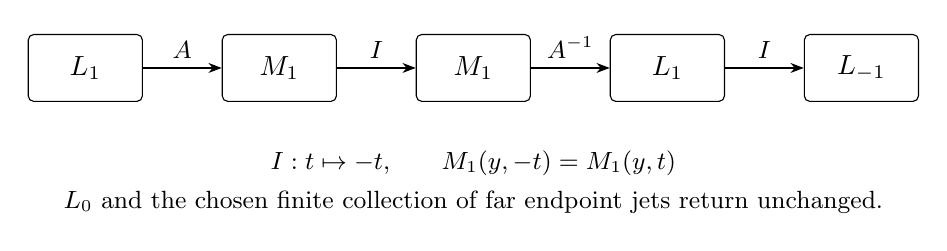
\begin{tikzpicture}[>=Stealth,node distance=1.0cm,
 state/.style={draw,rounded corners=2pt,minimum width=1.45cm,minimum height=.85cm}]
\node[state] (a) {$L_1$};
\node[state,right=of a] (b) {$M_1$};
\node[state,right=of b] (c) {$M_1$};
\node[state,right=of c] (d) {$L_1$};
\node[state,right=of d] (e) {$L_{-1}$};
\draw[->] (a)--node[above,font=\small] {$A$} (b);
\draw[->] (b)--node[above,font=\small] {$I$} (c);
\draw[->] (c)--node[above,font=\small] {$A^{-1}$} (d);
\draw[->] (d)--node[above,font=\small] {$I$} (e);
\node[font=\small,align=center,below=0.5cm of c]
 {$I:t\mapsto-t$,\qquad $M_1(y,-t)=M_1(y,t)$\\[3pt]
 $L_0$ and the chosen finite collection of far endpoint jets return unchanged.};
\end{tikzpicture}
\caption{The continuation operation in the no-patch argument.
The alternate transverse branch is even at glancing. For each prescribed
finite set of far indices, the path \(A\) is chosen to fix both signs of
those indices. The operation produces another root of the same endpoint
polynomial; it requires no common path for infinitely many indices.}
\label{fig:monodromy}
\end{figure}


Paths and generic basepoints can be chosen anew for each
finite selection.  The identities before and after are
identities of actual primary germs near real glancing,
and hence transport between those basepoints.

Apply \eqref{cont:monodromy-operation} to algebraicity of
\(L_1\) over the jets of \(L_0,L_b\).  It proves algebraicity
of \(L_{-1}\) over the same jets.  Translate this assertion.
From the endpoints of any interval \([B,B+b]\), the line
immediately to its left is now algebraic, as are all
interior lines by \Cref{thm:lens-lines}.  Differentiation
preserves algebraicity over a characteristic-zero
differential field.  Shift the interval one place left
and repeat; transitivity proves algebraicity of every
line to the left over the original endpoint jets.

Choose \(B>K+2\).  There is one fixed nonzero polynomial
over jets of \(L_B,L_{B+b}\) for a generic direction
coordinate of \(L_1\).  For each \(n\ge0\), first shear an
identity by \((y,t)\mapsto(y+2nt,t)\), apply
\eqref{cont:monodromy-operation} with far indices including
\(\pm(B+2n),\pm(B+b+2n)\), and shear back.  It sends
\[
L_{1-2n}\longmapsto L_{-1-2n}
\]
and fixes the original coefficient jets: the shear sends
\(L_{1-2n}\) to \(L_1\) and the coefficient fields to the selected
far indices, while the inverse shear returns those fields exactly.
For \(S_qF(y,t)=F(y+qt,t)\),
\(S_q(\partial_tF)=\partial_t(S_qF)-q\partial_y(S_qF)\);
thus the shear chain rules cancel with those of its inverse.
Inductively this
same polynomial has the direction coordinates of
\[
 L_1,L_{-1},L_{-3},L_{-5},\ldots
\]
as roots in the field of primary germs.
They are distinct: since
\(\Theta(y,t)=\phi(y)+O(t^2)\), the first \(t\)-derivative
of a generic slope coordinate of \(L_j\) is
\(j\phi'(y)\) times a nonzero chart factor.  A nonzero
polynomial over a field cannot have infinitely many
distinct roots.  This contradiction excludes a first
wall at or below \(H_1+\eta\) for generic real irrational
parameters in the neighborhood under consideration.

\paragraph{Transfer to the original real parameter.}
For every nearby irrational \(t_1\), the preceding
construction supplies a parameter neighborhood on which
\[
 h_L(t)\ge H_1+\eta
\]
for real \(t\) outside a countable exceptional set.
The increment \(\eta\) depends only on the initial patch.
A countable subcover covers all nearby irrational real
parameters.  Discarding their exceptional sets and the
countably many rational shifts yields the displayed
bound almost everywhere on an interval about \(t_0\).

Put \(M=H_1+\eta\).  On an upper half disk with diameter
in that interval, approximate the nonnegative lower
semicontinuous boundary values of \(h_L\) from below by
continuous functions supported away from the diameter
endpoints.  Superharmonic comparison and the
almost-everywhere bound give
\[
 h_L(t)\ge M\omega_+(t),
\]
where \(\omega_+\) is the harmonic measure of the diameter.
The lower half disk gives \(h_L\ge M\omega_-\).
Both harmonic measures tend to one near the interior
diameter point \(t_0\).  The small-circle supermean
inequality centered at \(t_0\), followed by shrinking
the circle, gives \(h_L(t_0)\ge M\).  This contradicts
\(h_L(t_0)=H_1\).

\paragraph{The same conclusion for impact patches.}
Suppose now that \(X\) has a joint patch through its
finite first wall at a real parameter.  At real
parameters \eqref{cont:width-equality} gives \(h_X=h_L\).
For nearby irrational shifts, forward and backward
translates
\[
 X(y+(j+1/2)t,t)
\]
of the patch supply enclosing impacts for every edge.
Choose a finite covering by phase boxes, enclosing indices
with at least two steps between them, and a common
narrower vertical band exactly as above.
\Cref{thm:lens-points}, with the analytic coefficient
\(A(t)\), supplies full-band joint polynomial equations
for the edge \(L(y,t)\), attached to the primary branch
on a common bottom strip.

These equations are exactly the input to the first part
of the argument.  Generic slices, root bounds and
monodromy turn a first obstruction into a finite defect.
Its exclusion still uses the line-endpoint identities of
\Cref{thm:lens-lines} and the evenness operation
\eqref{cont:monodromy-operation}; no additional point
identity is needed in that exclusion.  Thus
\(h_X(t)=h_L(t)\ge H_1+\eta\) almost everywhere on a
real interval.  Apply the same superharmonic transfer to
\(h_X\), using \Cref{prop:width-superharmonic}, to
contradict its value at the original parameter.
Real symmetry supplies the lower-wall assertion.
\end{proof}

\subsection{The boundary parametrization has the same natural wall}

The zero slice of the joint impact map is the boundary curve.
We must rule out the possibility that this slice continues
through a wall even though the two-variable family does not.
The argument first propagates glancing trajectories in steep
complex directions and then fills the remaining directions
by a family of quadratic disks.

\begin{corollary}[Natural boundary of the shape]
\label{cor:shape-natural-boundary}
Put \(H=h_X(0)=h_L(0)\).  The parametrization
\(\Gamma(y)=X(y,0)\) is meromorphic on
\[
 D_H=\{y\in\C:|\Im y|<H\}.
\]
If \(H<\infty\), it has no meromorphic continuation patch
through any point of either boundary line of \(D_H\).
Moreover, on its meromorphic domain,
\begin{equation}
 \frac{\det(\Gamma',\Gamma'')^4}
      {(\Gamma'\cdot\Gamma')^3}=c^2,
 \label{cont:intrinsic-normalization}
\end{equation}
where \(c\ne0\) is the normalized curvature constant from
the glancing construction.
\end{corollary}

\begin{proof}
At each strict upper subheight of \(H\), \(X\) has a joint
meromorphic extension near \(t=0\).  In generic affine
coordinates there is no polar component along the entire
zero slice: such a component would meet the initial
collar, where \(X(y,0)=\Gamma(y)\) is regular.
Restrictions to that slice are therefore meromorphic,
with only isolated exceptional points to remove in the
one-variable projective map.  They agree on overlaps by
the identity theorem.  Real symmetry supplies the lower
half, proving the first assertion.

On the original real arc the curvature normalization is
\(r(\phi(y))(\phi'(y))^3=c\).  Since the unit tangent is
\(e_\phi\), it gives
\[
 \Gamma'=\frac{c}{(\phi')^2}e_\phi,\qquad
 \Gamma'\cdot\Gamma'=\frac{c^2}{(\phi')^4},\qquad
 \det(\Gamma',\Gamma'')=\frac{c^2}{(\phi')^3}.
\]
These equations prove \eqref{cont:intrinsic-normalization}
on the real arc, hence meromorphically everywhere on
\(D_H\) and on any continuation patch.

Suppose \(H<\infty\) and a patch exists.  By real symmetry
we may use the upper edge.  Choose a regular point
\[
 s_{\rm edge}=x_*+\ii H
\]
of the patch where \(\Gamma'\cdot\Gamma'\) and
\(\det(\Gamma',\Gamma'')\) are both nonzero.  Such a point
exists after a small move along the edge: all exceptional
sets are isolated, since the corresponding meromorphic
functions are nonzero on the original real arc.
Shrink the patch so that \(\Gamma\), its normal, a local
normal angle \(\phi\), the inverse angle coordinate, and
the curvature radius are holomorphic and nondegenerate.
The normal is obtained from \(\Gamma'\) by a local square
root of its bilinear squared length; the angle then
comes from a local logarithm.  The intrinsic identity
\eqref{cont:intrinsic-normalization} shows that
\(r(\phi)(\phi')^3\) is a nonzero constant on this patch,
equal to \(c\) up to the local sign choices.  The zero
slice \(L(y,0)\) is its tangent, by continuation from below.

\paragraph{A regular starting segment.}
Choose a row slightly below \(H\), sufficiently close
that all short slanted segments with normalized vertical
component of absolute value at least \(1/3\), ending near
\(s_{\rm edge}\), remain inside the regular patch.  Their
starting points lie in a compact horizontal segment.
Choose the exact row height to avoid joint poles and
indeterminacies of \(L,X\) on \(t=0\) over this segment.
This is possible because in affine charts finite along
the segment there is no polar component equal to the
zero slice; joint exceptions intersect it discretely.
Compactness then gives a neighborhood of the segment
on which \(L,X\) are analytic for small complex \(t\).
Evenness gives the line angle expansion
\begin{equation}
 \Theta(y,t)=\phi(y)+O(t^2)
 \label{cont:patch-angle-expansion}
\end{equation}
uniformly there.

The rank-one identity identifies the nearby impact image
with the fixed regular curve arc traced on \(t=0\).
The reflection identity is its ordinary local reflection
law.  Thus the successive line angles, expressed in the
normalized coordinate
\[
 V=\phi^{-1}(\hbox{line angle}),
\]
satisfy the stationary recurrence of the local action
\(D\).  The support and all root branches are chosen
locally; the line angles are close enough that their
mean is the normal angle at the shared impact.

\paragraph{Cubic accuracy of the local recurrence.}
The same local Taylor calculation used for the normalized
action, now using constancy of \(r(\phi)(\phi')^3\), gives
\[
 \partial_1D(V,V+s)=\kappa s^2+O(s^4),
 \qquad \kappa\ne0\ \hbox{constant}.
\]
There is no cubic term.  Antisymmetry of \(D\) turns
stationarity at a node into equality of this expression
for the forward and backward increments.  Its analytic
square root is \(s\sqrt{\kappa+O(s^2)}\).  Choosing the
opposite root from the repeated previous node gives the
nonrepeated successor analytically and uniformly:
\begin{equation}
 V_{j+1}=2V_j-V_{j-1}
                +O\bigl((V_j-V_{j-1})^3\bigr).
 \label{cont:steep-recurrence}
\end{equation}
The offsets of the corresponding lines are also analytic,
being the endpoint momenta of the local generating
function \(\mathcal S\).

\paragraph{Propagation in steep directions.}
Assume \(|\Im t|\ge |t|/3\).  Replace \(t\) by \(-t\)
if necessary, using evenness, so that the step is upward.
For a target \(y\) near the edge choose \(N\) with
\(y-Nt\) in the starting neighborhood.  There is a uniform
bound \(N=O(1/|t|)\).  Initialize the recurrence with
\[
 V_0=y-Nt+O(t^2),\qquad
 V_1=y-(N-1)t+O(t^2),
\]
using \eqref{cont:patch-angle-expansion}.
If the step sizes stay at most \(2|t|\), each recurrence
error is \(O(|t|^3)\).  Summing the errors once gives
\[
 V_j-V_{j-1}=t+O(t^2),
\]
and summing a second time gives
\[
 V_j-\bigl(y-(N-j)t\bigr)=O(|t|),
 \qquad 0\le j\le N.
\]
These estimates close the assumed step bound for small
\(|t|\).  Choose the geometric paths with fixed slack in
the regular patch before shrinking \(|t|\); then every
iterate remains in that patch.

For locally constant \(N\), this construction is
holomorphic in \(y,t\).  Choices of different \(N\)'s
agree: take their starting points in a thin slab of
known analytic data, where the exact recurrence relates
all intervening indices, then apply uniqueness of the
nonrepeated successor.  It follows that the resulting
germs glue near the target and along a vertical corridor
down to the starting slab, uniformly for all steep
directions.  They are attached to the primary data on
a fixed lower part of that corridor.  At any chosen
strict subheight below \(H\), make \(|t|\) smaller if
needed so that uniqueness identifies them with the
already known primary branch.  The line construction
also gives \(X\) by the neighboring intersections.
All choices have been made in order: first the regular
patch and geometric slack, then the vertical travel
distance, and finally the allowed size of \(|t|\).

\paragraph{Quadratic disks fill the shallow directions.}
Choose \(\eta>0\) small compared with both the corridor
size and the depth of the starting row.  Next choose
a sufficiently small parameter radius \(r_0>0\).  Consider
the analytic disks
\begin{equation}
 t=r_0\zeta,\qquad
 y=x_*+\ii\sigma-\ii\eta\zeta^2+w,\qquad
 H-2\eta\le\sigma\le H,
 \label{cont:quadratic-disks}
\end{equation}
where \(w\) is a small complex transverse parameter.
At \(|\zeta|=1\), write \(\zeta=e^{\ii\theta}\).
On the near-real arcs \(|\sin\theta|<1/2\),
\[
 \Im y\big|_{w=0}
   =\sigma-\eta\cos(2\theta)
   \le H-\eta/2.
\]
These arcs therefore have joint primary data for small
\(r_0\).  On the remaining arcs,
\(|\Im t|/|t|\ge1/2\), so the steep continuation just
constructed applies with a strict margin over \(1/3\).
The continued germs glue to the primary ones on the
overlaps by their attachment below \(H\).
Compactness supplies a common annular collar in \(\zeta\)
and a common small disk in \(w\) on which the pullbacks
are meromorphic, throughout the indicated interval of
\(\sigma\).

At \(\sigma=H-2\eta\), the full disks have height at most
\(H-\eta\) for \(w=0\).  Hence they, and a small
neighborhood of them, already lie in the primary joint
domain when \(r_0\) is sufficiently small.
Increase \(\sigma\) in small steps.  The displacement of
one center is absorbed by the transverse \(w\)-disk, so
the full disks from the previous step give a nonempty
open seed at the next step.  Apply
\Cref{lem:meromorphic-hartogs,cont:disc-sweep} at each
step.  Uniqueness on the collars and on the seed
overlaps attaches the resulting extensions to the lower
branch throughout the ascent.

At \(\sigma=H\), the disk center \(\zeta=0\) gives a
joint meromorphic patch through
\((y,t)=(x_*+\ii H,0)\); varying \(w\) and \(\zeta\)
are local coordinates there because \(r_0\ne0\).
This contradicts \Cref{thm:no-patch}, applied to \(L\)
at the real parameter \(0\).  The supposed shape patch
cannot exist.  Real symmetry excludes a lower-edge
patch as well.
\end{proof}

\section{The shape strip and its intrinsic coordinate}
\label{sec:shapes}

Put
\[
 H=h_X(0)=h_L(0),\qquad D_H=\{s\in\C:|\Im s|<H\},
\]
where \(H=\infty\) is allowed. The meromorphic curve on this strip is
\(\Gamma(s)=X(s,0)\). By \Cref{cor:shape-natural-boundary}, if
\(H<\infty\), the primary curve has no meromorphic continuation through
any point of either boundary line of \(D_H\). We shall first dispose of
its isotropic tangencies. In their absence we shall construct a global
shape coordinate for every continued impact, including impacts at poles
of the affine curve.

\subsection{The meromorphic normal and isotropic centers}

Use isotropic affine coordinates
\[
 Z=x_1+\ii x_2,\qquad W=x_1-\ii x_2.
\]
On the original real curve put
\[
 a=e^{\ii\phi},\qquad f=\phi',\qquad
 c=r(\phi)f^3>0.
\]
The normalization of the phase coordinate gives
\begin{equation}
 \Gamma'=\frac{c}{f^2}e_\phi,\qquad
 Z'=\frac{\ii c a}{f^2},\qquad
 W'=-\frac{\ii c}{a f^2}.
 \label{shape:coordinate-derivatives}
\end{equation}
In particular,
\begin{equation}
 a^2=-\frac{Z'}{W'},\qquad
 f=\frac{1}{2\ii}\frac{(a^2)'}{a^2},\qquad
 a=\frac{f^2Z'}{\ii c}.
 \label{shape:normal-reconstruction}
\end{equation}
Read the first expression as a meromorphic function, then use its
logarithmic derivative in the second expression, and finally use the
third expression to choose the normal itself. These formulas extend
\(a\) and \(f\) meromorphically throughout \(D_H\); all their identities
with the original real data continue there. We call a zero or a pole of
\(a\) an \emph{isotropic center}.

We shall repeatedly use the intrinsic normalization
\begin{equation}
 \frac{\det(\Gamma',\Gamma'')^4}
 {(\Gamma'\mathbin{\cdot}\Gamma')^3}=c^2.
 \label{shape:intrinsic}
\end{equation}
This is the identity from \Cref{cont:intrinsic-normalization}. It also
follows immediately from \eqref{shape:coordinate-derivatives}:
\(\Gamma'\cdot\Gamma'=c^2/f^4\) and
\(\det(\Gamma',\Gamma'')=c^2/f^3\). Under a reparametrization
\(s=\sigma(u)\), the left side of \eqref{shape:intrinsic} is multiplied
by \(\sigma'(u)^6\).

\begin{lemma}[Rational profiles at an isotropic center]
\label{shape:isotropic-profile}
Suppose that \(a\) has a zero of order \(n\geq1\) at \(p\in D_H\).
Then \(n\ne3\). Set
\[
 D_+=n+3,\qquad D_-=3-n.
\]
There is a germ \(\xi(w)=w+O(1)\) at infinity such that both
\(\xi^{D_+}\) and \(\xi^{D_-}\) are rational. It satisfies
\begin{equation}
 \frac{\xi(w+1)^{D_+}-\xi(w)^{D_+}}
      {\xi(w+1)^{D_-}-\xi(w)^{D_-}}
 \frac{\xi(w-1)^{D_+}-\xi(w)^{D_+}}
      {\xi(w-1)^{D_-}-\xi(w)^{D_-}}
 =\left(\frac{D_+}{D_-}\right)^2
      \xi(w)^{2(D_+-D_-)}.
 \label{shape:profile-reflection}
\end{equation}
The corresponding assertion for a pole holds after interchanging
\(Z\) and \(W\).
\end{lemma}

\begin{proof}
Write \(z=s-p\). By \eqref{shape:normal-reconstruction},
\(f=n/(\ii z)+O(1)\). Integration of
\eqref{shape:coordinate-derivatives} therefore gives
\begin{equation}
 Z(s)-Z(p)\sim c_Z z^{n+3},\qquad
 W(s)-W_0\sim c_W z^{3-n},
 \label{shape:center-powers}
\end{equation}
with nonzero constants \(c_Z,c_W\). Here \(W_0=W(p)\) when \(W\) is
finite, and any fixed constant may be used when \(W\) has a pole. If
\(n=3\), the leading term of \(W'\) is a nonzero multiple of \(z^{-1}\),
which cannot be the derivative of a meromorphic function. This proves
\(n\ne3\).

At sufficiently close punctured points of the zero-parameter slice,
\(\Gamma\) is finite, regular and nonisotropic. Its local inverse,
together with the rank-one identity for \(X\), gives
\begin{equation}
 X(y,t)=\Gamma(v(y,t)),\qquad
 v(y,t)=y+\sum_{j\geq1}t^{2j}v_j(y).
 \label{shape:local-impact-series}
\end{equation}
The even powers follow from evenness of \(X\). Possible joint poles or
indeterminacies at points where the zero-slice restrictions are regular
form a discrete set on that slice. After shrinking the punctured disk,
there are no such exceptions. The coefficients in
\eqref{shape:local-impact-series} glue there. Recursively inverting one
of the coordinates of \(\Gamma\) shows that every \(v_j\) is
meromorphic at \(p\): at each order the new coefficient is divided only
by a nonzero meromorphic derivative of that coordinate.

To take a leading limit with \(z=s-p\) and \(t\) on the same scale,
meromorphy of the coefficients alone is not enough. We need the pole bound
\begin{equation}
 \ord_p v_j\geq1-2j.
 \label{shape:impact-coefficient-order}
\end{equation}
Under \(z=tw\), this keeps every formal term \(t^{2j}v_j(p+tw)\)
at order at least \(t\), just as for the leading displacement \(z\).
We prove the bound using the arc-minus-chord action, divided by \(c\),
between shape parameters \(s\) and \(s+h\):
\begin{equation}
 \mathcal D(s,s+h)=
 \int_s^{s+h}f^{-2}
 -\sqrt{\left(\int_s^{s+h}f^{-2}a\right)
              \left(\int_s^{s+h}f^{-2}a^{-1}\right)}
 =\frac{h^3}{24}+O(h^5).
 \label{shape:point-action}
\end{equation}
The square root initially has the arc-length branch. To check the cubic
coefficient, expand each integral at its midpoint. The difference
between the normalized second derivative of \(f^{-2}\) and the average
of those of \(f^{-2}e^{\pm\ii\phi}\) is \(f^2\). Multiplication by
\(f^{-2}\) leaves the constant coefficient \(1/24\).

Write \(\mathcal D(s,s+h)=\sum_m d_m(s)h^m\). Substituting
\(s=p+z\), \(h=z\eta\), the two chord integrals factor as
\(z^{3+n}\eta\) and \(z^{3-n}\eta\), respectively, times functions
holomorphic near \((z,\eta)=(0,0)\) and nonzero there after division by
\(\eta\). Their product has the square root \(z^3\eta\) times a
holomorphic unit, with the chosen glancing sign. Thus
\begin{equation}
 \ord_p d_m\geq3-m.
 \label{shape:action-coefficient-order}
\end{equation}
This argument concerns short segments away from the center; the
resulting coefficient identities are meromorphic identities at the
center.

Reflection implies stationarity of the sum of two consecutive actions
\(\mathcal D\) on the lifted impacts in
\eqref{shape:local-impact-series}. The arc terms telescope, and the
chosen square roots have velocities tending to the same unit tangent,
so their signs give the ordinary reflected branch. Divide this
stationary equation by \(t^3\). For a general function \(v\), its
leading expression is
\[
 -\frac14v_yv_{yy}.
\]
Indeed the cubic action contributes one eighth of the difference of
the squared previous and next increments. At order \(t^{2j}\), the new
coefficient consequently enters as \(-v_j''/4\).

Assign weight one to each of \(z,t\). Assuming
\eqref{shape:impact-coefficient-order} at preceding orders, the formal
truncation of \(v-p\) through order \(t^{2j-2}\) and its increments
have lower total degree at least one.
Taylor shifts by \(\pm t\) preserve this property. Composition of
\(d_m\) with \(v\) preserves its lower degree \(3-m\), because each
derivative lowers the allowed order by at most one. The endpoint
derivatives of the unnormalized action therefore have total lower
degree at least two. After division by \(t^3\), the forcing at order
\(t^{2j}\) has order at least \(-1-2j\) in \(z\). Only finitely many
terms enter any fixed coefficient, since every step has positive
\(t\)-order. Hence \(\ord_p v_j''\geq-1-2j\), which proves
\eqref{shape:impact-coefficient-order} because \(v_j\) is meromorphic.

Let \(P(z,t)\) be a constant-coefficient polynomial combination of the
affine coordinates of \(X(p+z,t)\). Suppose that its zero-slice
restriction has order \(b\in\Z\) and leading coefficient \(c_P\ne0\).
Composition with \eqref{shape:local-impact-series} and
\eqref{shape:impact-coefficient-order} show that its coefficient of
\(t^l\) has order at least \(b-l\). Consequently
\[
 z^{-b}P(z,z\lambda)
\]
is holomorphic near \((z,\lambda)=(0,0)\). Here is the convergence
point in this assertion. The expression is a meromorphic germ and its
formal expansion in \(\lambda\), with Laurent coefficients in \(z\),
belongs to \(\C[[z,\lambda]]\) by the order bound. A meromorphic germ
whose quotient is formally a power series is holomorphic: apply
Weierstrass preparation and division, after a generic linear change of
coordinates, to its numerator and denominator. More explicitly, replace
the denominator by a Weierstrass polynomial times a unit, and divide
the analytic numerator by that polynomial. The analytic remainder has
degree below the polynomial degree. Uniqueness of formal division,
compared with the given formal quotient, makes its formal remainder
zero. The analytic remainder is consequently zero as well, and the
analytic quotient is the desired germ; see
\cite[Theorem~6.1.1]{Hormander1990}. Thus formal nonnegative orders
imply genuine holomorphy in this instance.

Its restriction to \(z=0\) is rational in \(\lambda\), since it is the
ratio of the first nonzero homogeneous parts of a local numerator and
denominator after the substitution \(t=z\lambda\). Formally that
restriction equals
\[
 c_P\mathcal U(\lambda)^b,\qquad \mathcal U(0)=1,
\]
where \(\mathcal U\) collects the total-degree-one terms of \(v-p\).
Taking \(P=Z-Z(p)\), for which \(b=D_+>0\), supplies an analytic
\(D_+\)-th root near one and proves convergence of \(\mathcal U\).
Set \(\xi(w)=w\mathcal U(1/w)\). For sufficiently large \(R_0\),
\begin{equation}
 t^{-b}P(tw,t)\longrightarrow c_P\xi(w)^b
 \label{shape:rational-leading-limit}
\end{equation}
locally uniformly, with derivatives, on \(|w|>R_0\); the limit is
rational. Applying this to the two coordinates in
\eqref{shape:center-powers} proves rationality of the stated powers.

In isotropic coordinates reflection says that the product of the two
incident chord slopes, expressed as \(Z\)-increment divided by
\(W\)-increment, is the square of the tangent slope. Substitute
\eqref{shape:rational-leading-limit} at \(w,w-1,w+1\). The constants
\(c_Z/c_W\) cancel, and the derivative of \(\xi\) cancels from the
tangent ratio. This gives \eqref{shape:profile-reflection}, first near
infinity and then as an identity of rational functions. Interchanging
the isotropic coordinates treats a pole of \(a\).
\end{proof}

\begin{lemma}[Every isotropic center is simple]
\label{shape:simple-centers}
All zeros and poles of \(a\) in \(D_H\) are simple. At each such center
\(p\), the curve has the local symmetry
\begin{equation}
 \Gamma(2p-s)=\Gamma(s),\qquad a(2p-s)=-a(s).
 \label{shape:center-reflection}
\end{equation}
\end{lemma}

\begin{proof}
It suffices to consider a zero of order \(n\). Use the preceding
lemma and put
\[
 d=\gcd(D_+,|D_-|),\quad R=\xi^d,\quad
 \alpha=D_+/d,\quad\beta=D_-/d,\quad
 \rho(w)=\frac{R(w+1)}{R(w)}.
\]
Bezout's identity makes \(R\) rational from the rationality of the two
powers of \(\xi\). Since \(R(w)\sim w^d\),
\(\rho(w)=1+d/w+O(w^{-2})\). Thus \(\rho\) is a nonconstant rational
map of some degree \(s\geq1\), with \(\rho(\infty)=1\). Define
\[
 F(x)=\frac{x^\alpha-1}{x^\beta-1}.
\]
After cancellation of the common powers of \(R(w)\),
\eqref{shape:profile-reflection} becomes
\begin{equation}
 F(\rho(w+1))=
 \frac{(\alpha/\beta)^2}{F(1/\rho(w))}.
 \label{shape:rational-shift-equation}
\end{equation}
We use the Riemann--Hurwitz formula: a rational map of degree
\(s\) has total ramification \(2s-2\); see \cite{Forster1981}.

If \(n=2\), then \(\alpha=5,\beta=1\), so \(F\) is a polynomial
of degree four with simple zeros at the four nontrivial fifth roots
of unity. At each preimage by \(\rho\) of one of these four values,
the right side of \eqref{shape:rational-shift-equation} has a pole
whose order is the local multiplicity of that preimage. On the left,
a pole has order divisible by four. Thus all these multiplicities
are divisible by four. Each of the four fibers contributes at least
\(3s/4\) to ramification, giving total at least \(3s>2s-2\), a
contradiction.

Suppose next that \(n>3\). Write \(\gamma=-\beta>0\) and
\(m=\alpha-\gamma=6/d\geq1\). The function
\[
 F(x)=-x^\gamma\frac{x^\alpha-1}{x^\gamma-1}
\]
has a pole of order \(\alpha\) at infinity. The function on the
right of \eqref{shape:rational-shift-equation}, considered as a
function of \(\rho\), has a pole of order \(\gamma\) at infinity
and simple poles at the nontrivial \(\alpha\)-th roots of unity.
These roots are distinct from its other possible exceptional values,
since \(\gcd(\alpha,\gamma)=1\).

Group the finitely many poles of \(\rho\) into maximal runs
\(w_0,w_0+1,\ldots,w_0+\ell\), with respective orders
\(p_0,\ldots,p_\ell\). Comparing pole orders at the points of the
run gives
\[
 \alpha p_{j+1}=\gamma p_j\quad(0\leq j<\ell).
\]
At the preceding point \(w_0-1\), which is not a pole of \(\rho\),
\(\rho\) must take a nontrivial \(\alpha\)-th root with multiplicity
\begin{equation}
 \alpha p_0=m\sum_{j=0}^\ell p_j+\gamma p_\ell.
 \label{shape:pole-run-seam}
\end{equation}
The preceding points of different runs are distinct. Their
ramification contributions are their displayed multiplicities minus
one. If \(m\geq2\), \eqref{shape:pole-run-seam} shows that these
points alone contribute at least \(ms\geq2s\), a contradiction.

If \(m=1\) and \(\gamma\geq2\), coprimality in the recurrence
implies \(\gamma^\ell\mid p_\ell\). Therefore
\(\gamma p_\ell-1\geq\ell+1\). If \(N_P\) is the number of
distinct poles, the preceding points contribute at least \(s+N_P\),
while the poles themselves contribute \(s-N_P\). Again the total is
at least \(2s\). The only remaining possibility is
\(m=\gamma=1\), \(\alpha=2\). All preceding points then take the
single value \(-1\), and their total multiplicity, by
\eqref{shape:pole-run-seam}, is strictly larger than \(s\). This is
impossible for one fiber of a degree-\(s\) map. Together with the
exclusion of \(n=3\), these arguments leave only \(n=1\).

For \(n=1\) we have \(d=2,\alpha=2,\beta=1\). Equation
\eqref{shape:rational-shift-equation} reads
\[
 (1+\rho(w+1))(1+1/\rho(w))=4.
\]
Equivalently, \(2/(\rho-1)\) increases by one under translation.
A rational one-periodic function is constant, so
\[
 \frac{2}{\rho(w)-1}=w+b_0,
 \qquad R(w)=(w+b_0)(w+b_0+1).
\]
The second identity follows by comparing the shift ratios and the
asymptotic \(R(w)\sim w^2\). In particular \(\xi\) is not rational,
since \(\xi^2\) has two simple zeros.

Choose a local coordinate \(\zeta=z+O(z^2)\) such that
\(W-W_0=c_W\zeta^2\). If the expansion of \(Z\) in \(\zeta\)
had a first odd term of order \(j\), subtracting the preceding even
terms as a polynomial in \(W-W_0\) would give a polynomial
combination \(P\) with order \(j\). By
\eqref{shape:rational-leading-limit}, \(\xi^j\) would be rational.
Since \(j\) is odd and \(\xi^2\) is rational, Bezout's identity would
make \(\xi\) rational, a contradiction. Thus both coordinates of
\(\Gamma\) are even in \(\zeta\). The involution
\(\zeta\mapsto-\zeta\) induces a local symmetry \(\sigma\) of the
shape parameter, fixing \(p\) with derivative \(-1\).

By \eqref{shape:intrinsic}, \(\sigma'^6=1\) on regular points.
Its derivative is therefore constant, and \(\sigma(s)=2p-s\).
The tangent-ratio identity gives \(a(\sigma(s))^2=a(s)^2\).
The simple zero fixes the sign to be negative. This proves
\eqref{shape:center-reflection}; the pole case is identical after
interchanging \(Z,W\).
\end{proof}

\begin{theorem}[Classification in the presence of isotropic centers]
\label{thm:isotropic-classification}
If \(a\) has a zero or a pole in \(D_H\), the boundary is an ellipse.
\end{theorem}

\begin{proof}
A center is nonreal, since \(|a|=1\) on the real axis. If \(H<\infty\),
the symmetry \eqref{shape:center-reflection} extends by identity on
the overlap of \(D_H\) with its reflection about the center. That
overlap is connected. The reflected strip extends past one of the
edges of \(D_H\), giving a meromorphic continuation of \(\Gamma\)
through an edge arc. This contradicts
\Cref{cor:shape-natural-boundary}. Hence \(H=\infty\).

Real symmetry supplies the conjugate center, and composition of the
two center reflections supplies a nonreal period, in addition to
\(2\pi\). Thus \(a\) is a nonconstant elliptic function. Let
\(\Lambda\) be its full period lattice. Composing reflections about
any two centers shows that twice their difference belongs to
\(\Lambda\). Consequently all zeros and poles lie in the four
classes of one translate of \(\frac12\Lambda/\Lambda\). They are
all simple by \Cref{shape:simple-centers}. The degree of \(a\) on
\(\C/\Lambda\) is therefore at most two. It cannot be one, because
a degree-one meromorphic map from a torus to the sphere would be a
biholomorphism. Its degree is exactly two.

Riemann--Hurwitz now gives four simple ramification points. Their
branch values \(\beta_1,\ldots,\beta_4\) are distinct and finite:
a fiber of degree two cannot contain two ramification points, and
the poles of \(a\) are simple. The quotient
\[
 \frac{a'^2}{\prod_{j=1}^4(a-\beta_j)}
\]
has neither zeros nor poles on the torus. At a ramification point
both numerator and denominator have order two; at a simple pole
both have order minus four. Hence the quotient is a nonzero
constant. We have obtained
\begin{equation}
 a'^2=P(a),\qquad \deg P=4.
 \label{shape:elliptic-normal-equation}
\end{equation}
Differentiating \(a(2p-s)=-a(s)\) gives
\(a'(2p-s)=a'(s)\), so \(P(-a)=P(a)\). Thus \(P\) is even.
On the real curve,
\[
 f^2=-\frac{a'^2}{a^2}
   =C+B\cos(2\phi)+D\sin(2\phi)>0
\]
for real constants \(B,C,D\). Therefore
\(f^2=n_\phi^{\mathsf T}Nn_\phi\) for a real positive-definite
symmetric matrix \(N\). Positivity follows on all directions since
\(\phi\) runs once around the circle.

For \(q_N(\phi)=n_\phi^{\mathsf T}Nn_\phi\), direct differentiation
gives
\[
 \left(\sqrt{q_N}\right)''+\sqrt{q_N}
 =\frac{\det N}{q_N^{3/2}}.
\]
For example, use \(q_N'=2e_\phi^{\mathsf T}Nn_\phi\) and
\(q_N''=2\operatorname{tr}N-4q_N\), and evaluate the determinant of
\(N\) in the orthonormal basis \((n_\phi,e_\phi)\). It follows that
the support
\[
 h_0(\phi)=\frac{c}{\det N}\sqrt{n_\phi^{\mathsf T}Nn_\phi}
\]
has curvature radius \(c/f^3\), the radius of the given boundary.
This is the support of an ellipse. The difference \(h-h_0\) solves
\((h-h_0)''+(h-h_0)=0\), so it is a linear combination of
\(\cos\phi,\sin\phi\), precisely a translation of the support.
\end{proof}

\subsection{A global lift when the normal is nonisotropic}

For the rest of this section suppose that \(a\) has neither zeros
nor poles in \(D_H\). Since the strip is simply connected, it has a
holomorphic logarithm. Choose \(\phi\) consistently with the real
normal. Then \(\phi,f=\phi'\) are holomorphic, and
\[
 \phi(s+2\pi)=\phi(s)+2\pi.
\]
The affine curve can still have poles, caused by zeros of \(f\).
The following theorem controls the impact coordinate even there.

\begin{theorem}[The global shape lift]
\label{thm:shape-lift}
Unless the boundary is a circle, there is a single-valued holomorphic
function \(\mathfrak s\) on the joint tube
\begin{equation}
 \mathcal T=\left\{(y,t):t\text{ is in the parameter disk},\quad
 -h_X(\bar t)<\Im y<h_X(t)\right\}
 \label{shape:joint-tube}
\end{equation}
such that
\begin{equation}
 X(y,t)=\Gamma(\mathfrak s(y,t)),\qquad
 |\Im\mathfrak s(y,t)|<H.
 \label{shape:global-composition}
\end{equation}
It satisfies
\begin{equation}
 \mathfrak s(y,0)=y,\qquad
 \mathfrak s(y+2\pi,t)=\mathfrak s(y,t)+2\pi,\qquad
 \mathfrak s(y,-t)=\mathfrak s(y,t).
 \label{shape:lift-symmetries}
\end{equation}
It also obeys real symmetry,
\(\mathfrak s(\bar y,\bar t)=\overline{\mathfrak s(y,t)}\).
After shrinking the parameter disk, for every real \(t\) the real
map \(y\mapsto\mathfrak s(y,t)\) descends to an orientation-preserving
analytic circle diffeomorphism. The inequality in
\eqref{shape:global-composition} is void when \(H=\infty\).
\end{theorem}

\begin{proof}
Near real glancing, the regular parametrization of the curve and the
rank-one identity give the asserted lift. Its differential satisfies
\begin{equation}
 c^2\mathfrak s_y^6
  =\frac{\det(X_y,X_{yy})^4}{(X_y\mathbin{\cdot}X_y)^3},
 \qquad
 \frac{\mathfrak s_t}{\mathfrak s_y}
  =\frac{X_t\mathbin{\cdot}X_y}{X_y\mathbin{\cdot}X_y}.
 \label{shape:lift-differential}
\end{equation}
Remove the proper analytic sets on which the meromorphic quantities
needed here have poles, vanish in a denominator, or make the chosen
sixth root zero. The complement containing the initial germ is
connected: removing complex analytic sets of positive codimension
does not disconnect a domain. Along any path in this complement the
sixth root, the closed differential it determines, and its local
primitive continue. Closedness continues from the initial germ.
On every compact regular path the differential is finite, and its
\(y\)-component is nonzero.

The composition identity persists for as long as the continued
primitive lies in \(D_H\). If \(H<\infty\), it cannot first reach an
edge of that strip. At such a first point the primitive is still
finite and locally submersive. Complete it to local product
coordinates \((\mathfrak s,z)\), and restrict the meromorphic map
\(X\) to a generic constant-\(z\) section. The identity on the inner
side would then continue the primary \(\Gamma\) meromorphically
through its edge, contradicting
\Cref{cor:shape-natural-boundary}. Thus the primitive remains in
the strip throughout continuation. For \(H=\infty\) there is no edge
to encounter.

After return along a loop, the continued primitive has the form
\[
 \mathfrak s\longmapsto\omega\mathfrak s+b,
 \qquad \omega^6=1.
\]
It consequently induces the symmetry
\begin{equation}
 \Gamma(\omega s+b)=\Gamma(s)
 \label{shape:possible-monodromy}
\end{equation}
on the overlap of the two relevant strips. That overlap is
connected, being the intersection of two strips. If \(H<\infty\),
a nonreal \(\omega\) makes the transformed strip cross an edge of
\(D_H\). If \(\omega=\pm1\), the same is true when \(\Im b\ne0\).
In either case \eqref{shape:possible-monodromy} would give an edge
patch. Thus only \(\omega=\pm1\), \(b\in\R\) remain.

For \(H=\infty\), a nonreal \(\omega\) gives a nonreal period by
conjugating the real translation \(s\mapsto s+2\pi\) with the affine
symmetry in \eqref{shape:possible-monodromy}. A nonreal translation
is already such a period. If \(\omega=-1\) and \(\Im b\ne0\),
compose that reflection with its conjugate, which is also a symmetry
by reality, to obtain the nonreal period \(b-\bar b\).
A period of \(\Gamma\) is a period of \(a\) by
\eqref{shape:normal-reconstruction}. Such a nonreal period, together
with \(2\pi\), would make the entire holomorphic function \(a\)
doubly periodic and hence constant. This contradicts its real
winding. Again only the real possibilities remain.

Real embeddedness rules out a real reflection in
\eqref{shape:possible-monodromy} and makes a real translation an
integer multiple of \(2\pi\). We conclude that
\[
 v=e^{\ii\mathfrak s}
\]
is single-valued on the regular complement. When \(H<\infty\), both
\(v\) and \(1/v\) are locally bounded, in fact between the bounds
given by \(e^{\pm H}\). They extend holomorphically across the
removed analytic sets by the removable-singularity theorem. The
bounds remain strict by the maximum principle, since \(v\) is
nonconstant on the zero slice. Hence the extension is nonvanishing
and still has \(|\log|v||<H\).

For completeness we address the unbounded-strip case separately;
bounded removability is not available there. The differential
\(\dd\mathfrak s\) is already single-valued, because all its
monodromy is translational. It extends meromorphically by
\eqref{shape:lift-differential}. Indeed, if a single-valued
holomorphic function off an analytic set has a meromorphic sixth
power, multiply it by a local denominator of that power; the
result is bounded, since its sixth power is holomorphic, and is
therefore removable. Apply this to \(\mathfrak s_y\), then use the
second identity in \eqref{shape:lift-differential} for the other
component.

Write \(\Gamma(s)=G(e^{\ii s})\), where \(G\) is meromorphic on
\(\C^*\). At a generic smooth point of a possible polar divisor,
restrict to a transverse disk, with the center deleted. The
single-valued function \(v\) on this punctured disk cannot have an
essential singularity. If it did, the image of every punctured
neighborhood would be dense; choosing sequences approaching any
regular value \(w\in\C^*\) would force
\(G(w)\) to equal the projective limit of the meromorphic map
\(X=G(v)\). The nonconstant map \(G\) would be constant.

Suppose instead that \(v\) has a zero of finite order \(k\). In a
local coordinate, \(v(z)=z^k u(z)\), \(u(0)\ne0\). Meromorphic
affine coordinates of \(X\) grow at most like \(|z|^{-N}\).
Every sufficiently small nonzero \(w\) has preimages satisfying
\(|z|\asymp|w|^{1/k}\). The identity \(G(w)=X(z)\) gives
polynomial growth of the affine coordinates of \(G\) at zero, hence
meromorphic extension there. A pole of \(v\) gives the analogous
extension at infinity. Reality,
\(G(1/\bar w)=\overline{G(w)}\) in Euclidean coordinates, supplies
extension at the other end. Consequently \(G\) is rational.
Equations \eqref{shape:normal-reconstruction} then make \(a\)
rational in \(w=e^{\ii s}\). A rational function with no zeros or
poles on \(\C^*\) is \(Cw^k\); its real winding is one, so \(k=1\).
This makes \(f\) constant and the boundary a circle, the excluded
case.

It follows that \(v\) extends with a nonzero finite value on every
generic transverse disk. Therefore
\(\dd\mathfrak s=\dd v/(\ii v)\) has no pole on such a disk.
Generic transverse directions detect all leading polar coefficients
of a meromorphic one-form: a nonzero coefficient covector cannot
annihilate every direction having nonzero normal component.
Thus \(\dd\mathfrak s\) has no polar divisor. Removability in
codimension two makes it holomorphic throughout \(\mathcal T\).

Finally, \(\mathcal T\) is simply connected. Its vertical fibers in
\(y\) are intervals containing \(\Im y=0\), so vertical contraction
retracts it to \(\R\) times the parameter disk. For finite \(H\),
take a holomorphic logarithm of the nonvanishing extension of \(v\).
For infinite \(H\), take a primitive of the holomorphic closed
one-form \(\dd\mathfrak s\). Normalize by the original germ. This
gives the required single-valued lift. The composition and all
symmetries in \eqref{shape:lift-symmetries}, including real symmetry,
follow by identity from the initial domain. On the real phase circle,
\(\mathfrak s_y=1+O(t^2)\) uniformly. Shrinking the disk makes this
derivative positive for real \(t\); the degree-one periodicity then
gives the asserted circle diffeomorphism.
\end{proof}

\subsection{Zeros of the speed and the first displacement coefficient}

\begin{lemma}[Simple zeros and a holomorphic potential]
\label{lem:f-zeros}
Every zero of \(f\) in \(D_H\) is simple. At each such zero,
\(f''=0\). Consequently
\begin{equation}
 q=\frac{f''}{f}
 \label{shape:potential-definition}
\end{equation}
extends holomorphically throughout \(D_H\).
\end{lemma}

\begin{proof}
Suppose that \(f\) vanishes at \(s_0\) to order \(m\geq1\). Use
fixed tangent and normal coordinates for the angle \(\phi(s_0)\),
and write \(z=s-s_0\). Since
\(\phi(s)-\phi(s_0)\) has order \(m+1\), the tangent and normal
components of \(\Gamma'\) in
\eqref{shape:coordinate-derivatives} have leading orders
\(-2m\) and \(1-m\), respectively, with nonzero coefficients.
If \(m=2\), the normal derivative has a nonzero residue, contrary
to meromorphy. If \(m\geq3\), integration gives tangent and normal
coordinate poles of orders \(2m-1\) and \(m-2\).

By \Cref{thm:shape-lift}, the lift is holomorphic near \((s_0,0)\).
The equation \(\mathfrak s(y,t)=s_0\) defines
\(y=s_0+O(t^2)\). For sufficiently small \(t\ne0\), the two
neighboring shape coordinates at phase shifts \(\pm t\) are
\(s_0\pm t+O(t^2)\); their impacts are finite. Along the central
curve, the chord to the previous impact therefore has normal-to-tangent
slope of order at least \(m+1\). Its normal angle \(\theta\)
can be chosen holomorphically, and
\[
 d=\theta-\phi(\mathfrak s)
   =O\big((\mathfrak s-s_0)^{m+1}\big).
\]
For its signed offset \(p_{\rm chord}\), differentiation of
\(p_{\rm chord}=n_\theta\cdot\Gamma(\mathfrak s)\) gives
\begin{equation}
 \dd p_{\rm chord}\wedge\dd\theta
 =c f(\mathfrak s)^{-2}\sin d\,
       \dd\mathfrak s\wedge\dd d
 =\pm A(t)\,\dd y\wedge\dd t.
 \label{shape:chord-area}
\end{equation}
The final identity is the continued area identity
\eqref{eq:area-coefficient}; choosing a local orientation can change
only its sign. Since \(A(t)=ct/4+O(t^3)\), it is nonzero for small
\(t\ne0\).

Set \(z=\mathfrak s-s_0\) and write \(d=z^{m+1}b\).
Then \(\dd\mathfrak s\wedge\dd d
=z^{m+1}\dd\mathfrak s\wedge\dd b\). The left side of
\eqref{shape:chord-area} thus vanishes to order at least
\(-2m+(m+1)+(m+1)=2\), a contradiction. Hence \(m=1\).
At a simple zero write \(f=Az+Bz^2+O(z^3)\), \(A\ne0\).
Since \(a'=\ii fa\), we have \(a=a(s_0)+O(z^2)\). The residue
of \(a/f^2\) is \(-2a(s_0)B/A^3\). It vanishes because
\(\ii c a/f^2=Z'\) is a derivative of a meromorphic function.
Thus \(B=0\), which is \(f''(s_0)=0\). The asserted removability
of \(q\) follows.
\end{proof}

We now fix the harmless freedom to translate phase as a function of
\(t\). Let
\[
 b(t)=\frac{1}{2\pi}\int_0^{2\pi}
             (\mathfrak s(y,t)-y)\,\dd y.
\]
This is analytic and even, real for real \(t\), and vanishes at zero.
Precompose \(L,X,\mathfrak s\) with \(y\mapsto y-b(t)\), shrinking
the parameter disk if necessary. Periodicity and contour translation
then give
\begin{equation}
 \left\langle\mathfrak s(y,t)-y\right\rangle=0.
 \label{shape:mean-normalization}
\end{equation}
All rotation, area and symmetry identities are preserved. The two
widths acquire the same harmonic summand \(\Im b(t)\); hence the
width relation, superharmonic comparison and no-patch properties are
also preserved. We retain the previous notation for the normalized
data. Averaging on any horizontal row in the tube now gives
\(\langle\Im\mathfrak s\rangle=\Im y\). The shape constraint
therefore implies
\begin{equation}
 h_X(t)\leq H.
 \label{shape:width-bound}
\end{equation}

\begin{proposition}[The first impact displacement]
\label{shape:first-displacement}
For the normalization \eqref{shape:mean-normalization},
\[
 \mathfrak s(y,t)=y+t^2V(y)+O(t^4),
\]
where \(V\) is holomorphic and periodic on \(D_H\), has zero mean,
and satisfies
\begin{equation}
 V'=\frac{f^2+8q-\langle f^2+8q\rangle}{120}.
 \label{eq:V-coefficient}
\end{equation}
\end{proposition}

\begin{proof}
It suffices to calculate on real nonsingular data and then continue
by identity. In \eqref{shape:point-action} put
\(g=f^{-2}\), \(g_\pm=g e^{\pm\ii\phi}\). Midpoint integration
through the fourth derivative gives
\begin{equation}
 \mathcal D(s,s+h)
 =\frac{h^3}{24}+d_5(s+h/2)h^5+O(h^7).
 \label{shape:fifth-action}
\end{equation}
For clarity, define
\[
 B_j=\frac12\left(\frac{g_+^{(j)}}{g_+}
                         +\frac{g_-^{(j)}}{g_-}\right),\qquad
 C_2=2(g'/g)f+f'=-3f'.
\]
Multiplying the two midpoint integral expansions and taking the
glancing square root gives
\[
 d_5=g\left[
       \frac{g''''/g-B_4}{1920}
       -\frac{C_2^2}{2\cdot24^2}\right].
\]
Differentiating \(g_\pm\) explicitly yields
\[
 g''''/g-B_4=-8ff''+15(f')^2-f^4.
\]
The two \((f')^2\) contributions cancel, since
\(15/1920=9/(2\cdot24^2)\). Therefore
\begin{equation}
 d_5=-\frac{f^2+8q}{1920}.
 \label{shape:d5}
\end{equation}

At the middle impact \(s=\mathfrak s(y,t)\), the previous and next
shape increments are
\[
 h_-=t+t^3V'-\tfrac12t^4V''+O(t^5),\qquad
 h_+=t+t^3V'+\tfrac12t^4V''+O(t^5).
\]
The cubic term in the stationary action contributes
\(-t^5V''/4\). The fifth-order terms contribute
\(-5t^5d_5'+t^5d_5'\): the first part comes from differentiating
the increments and comparing the two midpoint values, and the
second from differentiating the midpoints. Hence stationarity at
order \(t^5\) reads
\[
 -V''/4-4d_5'=0.
\]
Substitute \eqref{shape:d5}, integrate once, and use periodicity of
\(V\) to determine the integration constant. This proves
\eqref{eq:V-coefficient}. The zero mean of \(V\) follows from
\eqref{shape:mean-normalization}.
\end{proof}

\section{Normalized chord equations and passage through cones}
\label{sec:cones}

We work in the nonisotropic alternative of
\Cref{thm:isotropic-classification}. Thus the shape curve has a holomorphic
normal on its shape strip, the impact lift is the function
\(\mathfrak s\) of \Cref{thm:shape-lift}, and
\[
 f=\phi',\qquad q=f''/f,\qquad
 M(s)=\max\{|f(s)|,|q(s)|^{1/2}\}.
\]
Both \(f\) and \(q\) are holomorphic by \Cref{lem:f-zeros}.
The phase normalization is \eqref{shape:mean-normalization}:
\(\langle\mathfrak s-y\rangle=0\). In particular,
\(h_X(t)\le H\) by \eqref{shape:width-bound}. We first write the billiard equation in a form that
remains analytic when the affine coordinates of the shape curve have
poles. We then use its small-field estimate to continue the lift toward a
finite boundary of the shape strip.

\subsection{Kernel division and the exact recurrence}

Fix a shape point \(s\), a nonzero small parameter \(t\), and a normalized
step \(J\); the second endpoint is \(s+tJ\). The variable \(u\) below is a
fast coordinate, and derivatives with respect to \(u\) are denoted by
primes. Set
\begin{equation}\label{cone:fast-fields}
 F(u)=t f(s+tu),\qquad Q(u)=t^2q(s+tu),\qquad F''=QF,
\end{equation}
and introduce the three potentials
\begin{equation}\label{cone:kernel-potentials}
 Q_0=Q,\qquad Q_\pm=Q\mp\frac{3\ii}{2}F'-\frac{F^2}{4}.
\end{equation}
For each potential, let \(k_j(u)\) be the solution of
\(k_j''=Q_jk_j\) with \(k_j(0)=0\), \(k_j'(0)=1\).
The normalized arc-minus-chord action is
\begin{equation}\label{cone:kernel-action}
 p(s,J;t)=\frac{\text{arc minus chord}}{ct^3}
 =\frac{k_0(J)-\sqrt{k_+(J)k_-(J)}}{F(0)F(J)}.
\end{equation}
Here and below the square root is the branch continued from short real
chords at glancing. The letter \(p\) in this Section denotes this action,
not the offset of an unoriented line.

To verify \eqref{cone:kernel-action}, put
\[
 g_0=F,\qquad
 g_\pm(u)=F(u)\exp\left(\mp\frac{\ii}{2}\int_0^u F(v)\,\dd v\right).
\]
Direct differentiation, using \(F''=QF\), gives
\(g_j''=Q_jg_j\). Where \(g_j\ne0\), reduction of order gives
\begin{equation}\label{cone:reduction-order}
 k_j(J)=g_j(0)g_j(J)\int_0^Jg_j(u)^{-2}\,\dd u.
\end{equation}
The identity extends meromorphically across zeros. In the formula
\(\Gamma'=ce_\phi/f^2\), the arc integral is \(c\int f^{-2}\), and the
squared chord length is the product of the integrals of
\(cf^{-2}e^{\ii\phi}\) and \(cf^{-2}e^{-\ii\phi}\).
Substitution of \eqref{cone:reduction-order}, including the change
\(\dd s=t\,\dd u\), gives \eqref{cone:kernel-action} first for regular real
short chords and then by analytic continuation.

\begin{lemma}[Analytic kernel division]\label{lem:kernel-division}
Let \(Q\) be holomorphic on a fixed neighborhood of an integration
segment from \(0\) to \(J\). Regard \(Q\), \(J\), and the initial data
\(F(0),F'(0)\) for \(F''=QF\) as variables. Near zero initial data and a
pair \((Q,J)\) for which \(k_0(J)\ne0\), the right side of
\eqref{cone:kernel-action}, with the square root equal to \(k_0(J)\) at
zero initial data, extends holomorphically through
\(F(0)F(J)=0\). This extension is even in \(F\). Its bounds and analytic
dependence, including derivatives on smaller neighborhoods, are uniform
on compact sets of admissible \((Q,J)\).

In particular, for \(J\) in a fixed sufficiently small neighborhood of
\(1\), and small \(Q,F(0),F'(0)\),
\begin{equation}\label{cone:small-action}
 p-\frac{J^3}{24}
 =O\left(\|Q\|+|F(0)|^2+|F'(0)|^2\right).
\end{equation}
The same estimate holds for any fixed number of \(J\)-derivatives on a
smaller neighborhood.
\end{lemma}

\begin{proof}
The integral equation
\[
 k_j(u)=u+\int_0^u(u-v)Q_j(v)k_j(v)\,\dd v
\]
proves analytic dependence and uniform bounds by its uniformly convergent
Picard series. The same argument applies to \(F\) and to a moving
endpoint \(J\), provided the segments and their small thickenings remain
in the fixed domain.

Suppose first that \(F(0)=0\). If \(F\not\equiv0\), uniqueness gives
\(g_j=g_j'(0)k_j\), and
\(g_+'(0)g_-'(0)=F'(0)^2\). Since
\(g_+(J)g_-(J)=F(J)^2=F'(0)^2k_0(J)^2\), it follows that
\(k_+(J)k_-(J)=k_0(J)^2\). The conclusion also holds when \(F\equiv0\).
If instead \(F(J)=0\), apply the same argument to kernels started at
\(J\). The value at \(0\) of such a backward kernel is \(-k_j(J)\):
this follows by evaluating the constant Wronskian of the forward and
backward kernels at both endpoints. The two signs cancel in their
product, and the same identity follows.

At zero initial data, \(k_+k_-=k_0^2\ne0\). Consequently the square root
agreeing with \(k_0\) is analytic nearby. On each of the two zero
hyperplanes just considered it agrees with \(k_0\), by uniqueness of
that local branch. The map from initial data to endpoint data is
\[
 (F(0),F'(0))\longmapsto(F(0),F(J)),
\]
whose determinant is \(k_0(J)\). Its coordinates are therefore
independent. An analytic function vanishing on both coordinate
hyperplanes is divisible by their product, as is seen by its convergent
power series. This proves the claimed extension. Cauchy estimates in
these two coordinates prove locally uniform bounds for the quotient
and its derivatives, also when \(Q\) and \(J\) vary.

Replacing \(F\) by \(-F\) interchanges \(k_+\) and \(k_-\), so the
quotient is even. At \(F=Q=0\), its value is \(J^3/24\), as follows by
taking \(F\) to be a small constant in the formula computed below.
Evenness removes the terms linear in the initial data; analytic
interpolation from \(0\) to \(Q\) bounds the remaining constant term by
\(O(\|Q\|)\). This proves \eqref{cone:small-action} and its derivative
versions.
\end{proof}

For consecutive endpoints \(s_-\), \(s=s_-+tJ_-\), and \(s+tJ\),
stationarity of the sum of the two actions is exactly
\begin{equation}\label{cone:normalized-recurrence}
 p_J(s,J;t)-t p_s(s,J;t)=p_J(s_-,J_-;t).
\end{equation}
Indeed the derivative in the final endpoint of
\(ct^3p(s_-,(s-s_-)/t;t)\) is \(ct^2p_J\), whereas the derivative in the
initial endpoint of \(ct^3p(s,(s_+-s)/t;t)\) is
\(ct^3p_s-ct^2p_J\). Thus \eqref{cone:normalized-recurrence} has no
uncontrolled remainder. By \Cref{lem:kernel-division} it also makes
sense at the exceptional affine points of the curve.

\subsection{The two frozen actions}

The limits needed later are constant fast fields satisfying \(FQ=0\).
For \(F=\lambda\), \(Q=0\), set \(z=\lambda J/2\). Here
\(k_0(J)=J\) and \(k_\pm(J)=2\sin z/\lambda\). Consequently the action
and its energy \(E=Jp_J-p\) are
\begin{equation}\label{eq:frozen-F-energy}
 p_F(\lambda,J)=\frac{J}{\lambda^2}-\frac{2\sin z}{\lambda^3},
 \qquad
 E_F(\lambda,J)=\frac{2(\sin z-z\cos z)}{\lambda^3}.
\end{equation}
For \(F=0\), \(Q=\lambda^2\), the analytically divided action is
\begin{equation}\label{eq:frozen-Q-energy}
 p_Q(\lambda,J)=\frac{J}{2\lambda^2}-\frac{\tanh z}{\lambda^3},
 \qquad
 E_Q(\lambda,J)=\frac{\tanh z-z\operatorname{sech}^2z}{\lambda^3}.
\end{equation}
All quotients have their continuous values at \(\lambda=0\).
For the second calculation, take \(F=\eta e^{\lambda u}\), which solves
\(F''=\lambda^2F\), and expand the arc and chord in \(\eta\). The common
term of order \(\eta^{-2}\) cancels. More explicitly, put
\[
 A(u)=\int_0^u e^{\lambda v}\,\dd v,
 \qquad I_j=\int_0^J e^{-2\lambda u}A(u)^j\,\dd u.
\]
The two chord factors are
\(\eta^{-2}(I_0\pm\ii\eta I_1-\eta^2I_2/2+O(\eta^3))\).
Their product is
\(\eta^{-4}(I_0^2+\eta^2(I_1^2-I_0I_2)+O(\eta^4))\), so subtraction
from the arc \(\eta^{-2}I_0\), with the glancing square root, leaves
\((I_2-I_1^2/I_0)/2+O(\eta^2)\). Since
\(A(u)=(e^{\lambda u}-1)/\lambda\), the limit is
\[
 \frac1{2\lambda^2}
 \left(J-\frac{\left(\int_0^J e^{-\lambda u}\,\dd u\right)^2}
 {\int_0^J e^{-2\lambda u}\,\dd u}\right)
 =\frac{J}{2\lambda^2}-\frac{\tanh(\lambda J/2)}{\lambda^3}.
\]
Lemma~\ref{lem:kernel-division} identifies this limit with the analytic
extension at \(F=0\).

For later use, the expansions at zero are
\begin{align}
 p_F&=\frac{J^3}{24}-\frac{\lambda^2J^5}{1920}+O(\lambda^4J^7),&
 E_F&=\frac{J^3}{12}-\frac{\lambda^2J^5}{480}+O(\lambda^4J^7),
 \label{cone:F-series}\\
 p_Q&=\frac{J^3}{24}-\frac{\lambda^2J^5}{240}+O(\lambda^4J^7),&
 E_Q&=\frac{J^3}{12}-\frac{\lambda^2J^5}{60}+O(\lambda^4J^7).
 \label{cone:Q-series}
\end{align}

\begin{lemma}[Convergence to a frozen action]\label{cone:profile-action-convergence}
Fix a compact path of frozen states from the small-field germ to a
finite point of one of the two displayed actions above, avoiding kernel
and root degeneracies, with \(J\ne0\) and \(p_{JJ}\ne0\) at its endpoint.
Suppose analytic fast fields satisfying \(F''=QF\) converge locally
uniformly to those frozen states on complex neighborhoods of the path
and of all its swept integration segments. Continue their glancing
square-root germs along
the corresponding perturbed path. Their actions then converge
analytically, with all derivatives on smaller neighborhoods of the
endpoint, to the frozen action on that fixed continued sheet. The
endpoint alone does not select a sheet after an arbitrary loop.
\end{lemma}

\begin{proof}
In the first case,
\(p_{JJ}=\sin z/(2\lambda)\); hence its nonvanishing excludes the zero of
\(k_\pm\), while \(k_0=J\ne0\). The ordinary quotient formula and
analytic dependence of kernels apply. In the second case,
\[
 p_{JJ}=\frac{\tanh z\,\operatorname{sech}^2z}{2\lambda},\qquad
 k_0=k_+=k_-=\frac{\sinh(2z)}{\lambda}.
\]
A zero of this last kernel either has \(\sinh z=0\), when
\(p_{JJ}=0\), or \(\cosh z=0\), when the displayed branch is not finite.
Thus the division lemma applies. The limiting case \(\lambda=0\) has
\(p_{JJ}=J/4\). A compact path can be covered by finitely many of these
analytic neighborhoods. Uniqueness of the square root on each overlap
tracks the chosen branch, and Cauchy estimates give convergence of all
derivatives.
\end{proof}

\subsection{Continuation in cones of arbitrary fixed aperture}

For this subsection suppose \(H<\infty\). Depth always means distance
below the upper edge:
\[
 \delta=H-\Im y,\qquad \delta_s=H-\Im s.
\]
The lower edge is treated by real symmetry.

\begin{theorem}[Cone passage]\label{thm:cone}
Fix \(1/2<\alpha<1\), a finite target aperture \(m_0\), and a fixed
\(\delta_b\in(0,H/2)\). There is an input aperture \(L\), depending on
\(\alpha\) and \(m_0\), with the following property. Fix \(K<\infty\),
let \(d\to0\), choose real centers \(x_0\), and let \(0<r\le Kd\).
Suppose
\begin{equation}\label{cone:input}
 rM(s)\le\eps(d/\delta_s)^\alpha
 \quad\text{if}\quad
 d/10\le\delta_s\le\delta_b,
 \quad |\Re s-x_0|\le L\delta_s.
\end{equation}
For sufficiently small \(\eps>0\) and then sufficiently small \(d\),
the lift continues jointly holomorphically along vertical paths from a
fixed lower row throughout
\begin{equation}\label{cone:target}
 d<\delta<\delta_*,\qquad
 |\Re y-x_0|<m_0\delta,\qquad
 |t|<r(\delta/d)^\alpha,
\end{equation}
where \(\delta_*>0\) is fixed. With
\(B=1+(\eps/r)d^\alpha\), it satisfies
\begin{equation}\label{cone:passage-estimate}
 |\mathfrak s(y,t)-y|
 \le C B^2|t|^2\delta^{1-2\alpha}.
\end{equation}
The relative depth error is small, so these continuations remain in the
shape strip, and they agree with the original lift wherever the latter
is defined below them.

The input aperture can be chosen independently of \(K\). Once it
contains the fixed geometric enlargements described in the proof, the
constant \(C\) and the smallness requirement on \(\eps\) can be chosen
independently of the target aperture. They may depend on \(K\),
\(\alpha\), and the fixed lower-strip data.
\end{theorem}

\begin{figure}[t]
\centering
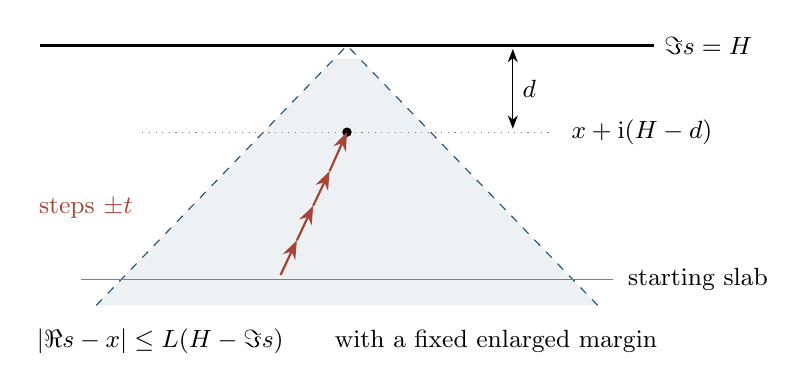
\begin{tikzpicture}[>=Stealth,x=1.3cm,y=1.1cm]
\fill[deepblue!8] (-.12,2.85)--(-2.45,0)--(2.45,0)--(.12,2.85)--cycle;
\draw[thick] (-3,3)--(3,3) node[right,font=\small] {$\Im s=H$};
\draw[deepblue,dashed] (-2.45,0)--(0,3)--(2.45,0);
\draw[gray] (-2.6,.30)--(2.6,.30);
\node[font=\small,anchor=west] at (2.65,.30) {starting slab};
\draw[gray,dotted] (-2.0,2)--(2.0,2);
\fill (0,2) circle (1.7pt);
\node[font=\small,anchor=west] at (2.10,2) {$x+\ii(H-d)$};
\draw[<->] (1.62,2.04)--node[right,font=\small] {$d$} (1.62,2.96);
\draw[->,warmred,thick] (-.65,.35)--(-.49,.75);
\draw[->,warmred,thick] (-.49,.75)--(-.33,1.15);
\draw[->,warmred,thick] (-.33,1.15)--(-.17,1.55);
\draw[->,warmred,thick] (-.17,1.55)--(0,2);
\node[font=\small,anchor=east,warmred] at (-2,1.12) {steps $\pm t$};
\node[font=\small,align=center] at (0,-.42)
 {$|\Re s-x|\le L(H-\Im s)$\qquad with a fixed enlarged margin};
\end{tikzpicture}
\caption{A cone passage begins in known analytic data and follows steep
increments toward the chosen depth. Local error bounds are summed in
depth, with exponent greater than \(1/2\). Enlarging a fixed aperture
provides geometric margin without changing the local constants.
Parameter disks subsequently fill the directions close to real increments.}
\label{fig:cone}
\end{figure}


\begin{proof}
We give separately the recurrence argument in steep parameter
directions, illustrated in \Cref{fig:cone}, and the analytic-disk argument that fills the remaining
directions.

Fix a small number \(\gamma>0\). Suppose first that
\(|\Im t|\ge\gamma|t|>0\). By evenness in \(t\), use whichever of
\(t,-t\) moves upward. Start in a fixed slab about depth
\(\delta_b/2\), where joint analyticity and the phase normalization give
\[
 \mathfrak s-y=O(t^2),\qquad
 \frac{\mathfrak s(y+t,t)-\mathfrak s(y,t)}{t}=1+O(t^2)
\]
with derivative bounds uniform in the real coordinate modulo its
period. The largest parameters in the construction tend to zero,
since \(r d^{-\alpha}\le Kd^{1-\alpha}\to0\).

Follow the exact recurrence toward the target, denoting successive
unperturbed depths by \(x_j\). They decrease by \(|\Im t|\). We allow
here the slightly larger range
\(x_j\ge d/2\), \(|t|\le10r(x_j/d)^\alpha\), which will be useful in
the disk construction. Suppose inductively that position errors are a
small fraction of the depths and that normalized steps are close to
\(1\). The shape fields on every required segment and a small
thickening satisfy
\[
 |F(0)|+|F'(0)|\le C_K|t|Bx_j^{-\alpha},\qquad
 \|Q\|\le C_K|t|^2B^2x_j^{-2\alpha}.
\]
To see the derivative estimate, apply Cauchy on a disk of radius a
small fixed fraction of \(x_j\). Although \(|t|/x_j\) need not tend to
zero, it is bounded by a constant depending on \(K\). Consecutive
depths are therefore comparable, with constants depending on \(K\),
and the thickenings may be taken with smaller such fractions. They
remain above depth \(d/10\). Their horizontal displacements lie in the
direction cone of slope at most \(1/\gamma\), with a fixed extra
margin. Increasing the input aperture by this fixed geometric amount
suffices; reducing the thickness when \(K\) increases does not require
a larger aperture.

The small parameter in the kernel estimates is bounded by
\[
 |t|Bx_j^{-\alpha}
 \le C\bigl(\eps+rd^{-\alpha}\bigr).
\]
Thus \Cref{lem:kernel-division} applies uniformly. If
\(a(s,J;t)=p(s,J;t)-J^3/24\), then
\begin{equation}\label{cone:action-estimates}
 |\partial_J^\nu\partial_s^\mu a|
 \le C_{K,\mu,\nu}|t|^2B^2x_j^{-2\alpha-\mu}
\end{equation}
for the finitely many derivatives used below. The \(s\)-derivative
bounds follow by Cauchy on the same thickenings.

Evaluate \eqref{cone:normalized-recurrence} with the trial new step
\(J=J_-\). The cubic contributions cancel. The difference of
\(a_J\) at the two adjacent basepoints, together with \(ta_s\), is at
most
\(C_K|t|^3B^2x_j^{-2\alpha-1}\). The derivative of the equation in
the new \(J\) is \(J/4+o(1)\), uniformly bounded away from zero.
The analytic implicit function theorem therefore supplies a unique
nearby step, with
\begin{equation}\label{cone:one-step}
 |J-J_-|\le C_K|t|^3B^2x_j^{-2\alpha-1}.
\end{equation}
For \(\beta>1\), comparison with an integral on the depth mesh gives
\[
 |t|\sum_{x_j\ge x}x_j^{-\beta}\le C_{K,\gamma,\beta}x^{1-\beta}.
\]
The possible final summand is controlled because \(|t|/x\) is bounded.
Summing \eqref{cone:one-step} first, and then summing the position
increments \(t(J-1)\), gives
\begin{equation}\label{cone:steep-estimates}
 |J-1|\le C_K|t|^2B^2x^{-2\alpha},\qquad
 |\mathfrak s-y|\le C_K|t|^2B^2x^{1-2\alpha}.
\end{equation}
The second sum uses \(2\alpha>1\). Initial errors from the fixed slab
are absorbed because \(B\ge1\). Moreover
\[
 \frac{|\mathfrak s-y|}{x}+|J-1|
 \le C_K\bigl(\eps+rd^{-\alpha}\bigr)^2,
\]
which closes the induction after the prescribed order of choices.

These recurrences define analytic germs in \((y,t)\). Locally choose a
fixed integer number of steps back into the starting slab, where both
initial neighbors are known. Two such choices agree by uniqueness of
the near-identity recurrence. They consequently give analytic
continuation from below on every steep sector under discussion.

We now fill all parameter directions. Call a germ reached if it is
obtained by continuing from the fixed lower row along the vertical path
with \(\Re y\) and \(t\) fixed. Reached germs form a single-valued
holomorphic function on their open domain: nearby parallel paths are
compared through a finite chain of the same germs from below. The steep
continuations just constructed agree with these germs. Work with
\[
 U(y,t)=\frac{\mathfrak s(y,t)-y}{t^2},
\]
which is regular at \(t=0\) on the initial domain and on its
continuations.

Choose a large fixed \(D_0\) with \(D_0^\alpha>10\), then a sufficiently
small fixed \(\gamma\). For a target \((y_c,t_c)\) of depth \(\delta\),
put \(R=r(\delta/d)^\alpha\). Since \(|t_c|<R\), the circle
\(t=t_c+3R\zeta\), \(|\zeta|=1\), meets the nonsteep sector only on
two uniformly short arcs. There is a polynomial \(g\), with
\(g(0)=0\), such that
\begin{equation}\label{cone:disk-bending}
 |g(\zeta)|\le C_0\delta,
 \quad \Im g\le\delta/4\ \text{on the circle},
 \quad \Im g\le-D_0\delta\ \text{on those arcs and a collar}.
\end{equation}
Here \(C_0\) is fixed independently of the target aperture. For
completeness, choose smooth negative bumps equal to a sufficiently
large negative constant on the two arcs and supported in slightly
larger short intervals. Add a constant to make their mean zero.
The intervals can be made so short that the added constant is less
than \(1/8\). Approximate the resulting smooth function, with a fixed
strict margin in its inequalities, by a real trigonometric polynomial
of mean zero. It is the boundary imaginary part of an analytic
polynomial vanishing at zero. Multiplication by \(\delta\) gives
\eqref{cone:disk-bending}. The centers of the arcs and
\(t_c/(3R)\) range over a compact set with modulus at most \(1/3\),
so the bump widths and polynomial degree can be fixed uniformly.
This also bounds the conjugate real part by \(C_0\delta\).

Increase an auxiliary target aperture \(m\ge m_0\) so that
\[
 m+C_0<mD_0.
\]
Choose \(L\) to contain this aperture, the shifts by \(C_0\delta\),
and the steep paths and thickenings above, all with fixed slack. We
induct from a sufficiently small fixed depth down through successive
bands whose depth thresholds are halved. In a new band use the disks
\begin{equation}\label{cone:disks}
 t=t_c+3R\zeta,\qquad y=y_c+g(\zeta)+w,
 \qquad |\zeta|\le1,
\end{equation}
where \(w\) is a small complex parameter. On the nonsteep boundary
arcs the depth is at least \(D_0\delta\). They are therefore in the
previous all-direction domain; the inequality
\(D_0^\alpha>10\) supplies the parameter margin, and
\(m+C_0<mD_0\) supplies the aperture margin. On the remaining arcs,
steep continuation applies at depth at least \(\delta/2\), with the
larger parameter range already allowed. Slight collars of the arcs
have the same properties.

Start \(y_c\) lower by a fixed sufficiently large multiple of
\(\delta\); then the entire disk and a neighborhood lie in the
previous domain. Raise \(y_c\) to its target value in small steps.
The holomorphic disk-continuation principle in
\Cref{lem:meromorphic-hartogs,cont:disc-sweep}, with the parameter \(w\),
continues \(U\) over the disks and identifies the resulting central
germ with vertical continuation from below.

There is no growth of the estimate with the number of bands. If the
inductive bound is \(A B^2x^{1-2\alpha}\), its value on a previous-domain
arc of depth \(x\ge D_0\delta\) is at most
\(A D_0^{1-2\alpha}B^2\delta^{1-2\alpha}\), with the fixed factor
\(D_0^{1-2\alpha}<1\). On a steep arc
\eqref{cone:steep-estimates} gives an independent constant times
\(B^2\delta^{1-2\alpha}\). Choose \(A\) once larger than that constant
and the initial lower-strip constant. Maximum modulus on each disk
retains the same \(A\). Starting the induction at a sufficiently small
fixed depth keeps its lower dips below \(\delta_b\); a partial last
band reaches any \(\delta>d\). This proves
\eqref{cone:passage-estimate}.

The constants in the depth sums, field bounds, and maximum-modulus
argument depend only on the fixed local margins. They do not depend
on how far the cone extends horizontally. Initial data are uniform
modulo the real period. Thus increasing a target aperture only
increases the input aperture needed to contain the indicated
geometric enlargements; it does not enlarge the estimate constant or
change the smallness choice. The relative-error estimate already
proved keeps the image below the upper shape edge and, after reducing
\(\delta_*\), above the lower edge.
\end{proof}

\begin{remark}[Reference heights]\label{cone:reference-height}
The local construction in \Cref{thm:cone} does not use the assertion that
\(H\) is a singularity height. It remains valid with a reference height
\(h\) in place of \(H\), provided the stated cone and its thickenings
are contained in the actual shape domain, lower-row initial data are
available, and the relative-error bound keeps the constructed lift in
that domain. In a rescaled sequence this formulation is applied on
fixed compact sets, with thresholds allowed to depend on the chosen
finite aperture. The constants in the estimate remain independent of
that aperture. A statement about the global width still uses the
actual first boundary of the phase domain, as explained next.
\end{remark}

\subsection{Quiet profiles and their consequences}

At a real parameter \(t\), any passage in \Cref{thm:cone} gives a global
lower bound on \(h_X(t)\). Indeed, if the original phase strip ended at
an earlier height, the local identity
\(X(y,t)=\Gamma(\mathfrak s(y,t))\), valid jointly in \((y,t)\) and with
\(|\Im\mathfrak s|<H\), would give a joint meromorphic patch through
that first edge. This contradicts \Cref{thm:no-patch}. This argument
uses the no-patch assertion only at a real physical parameter.

\begin{corollary}[Coarse bounds and quiet profiles]\label{cor:quiet-cone}
Let \(d_n\to0\), \(b_n\ge1\), and \(x_n\in\R\). Suppose, on a
sufficiently large fixed cone starting at depth \(d_n\), that
\begin{equation}\label{cone:coarse-bound}
 \frac{d_n}{b_n}M(s)\le C(d_n/\delta_s)^\alpha,
 \qquad \frac12<\alpha<1.
\end{equation}
The following statements hold; whenever an arbitrary fixed aperture is
used, the hypothesis is required on its corresponding fixed
enlargement.
\begin{enumerate}[label=\textup{(\roman*)}]
\item On a strictly coarser cone, starting at a fixed sufficiently large
multiple of \(d_n\), there is a passage with parameter radius
\(c(d_n/b_n)(\delta/d_n)^\alpha\), and
\begin{equation}\label{cone:coarse-error}
 |\mathfrak s-y|
 =O\left(b_n^2|t|^2d_n^{2\alpha-2}\delta^{1-2\alpha}\right).
\end{equation}
Equivalently, for
\(Y=(y-x_n-\ii H)/d_n\),
\(S=(\mathfrak s-x_n-\ii H)/d_n\), and \(T=tb_n/d_n\),
\[
 |S-Y|\le C|T|^2(-\Im Y)^{1-2\alpha}
\]
far enough down at each bounded \(T\).
\item Suppose in addition that
\begin{equation}\label{cone:quiet-profile}
 \frac{d_n}{b_n}M(x_n+\ii H+d_n S)\longrightarrow0
\end{equation}
uniformly on every compact subset of \(\Im S<0\).
For every \(c_1,T_1>0\), lift passages reach depth \(c_1d_n\) for all
\(|t|\le T_1d_n/b_n\), for large \(n\). At real parameters, with
\(\Delta(t)=H-h_X(t)\),
\begin{equation}\label{cone:quiet-width}
 \sup_{|T|\le T_1}\frac{\Delta(Td_n/b_n)}{d_n}\longrightarrow0.
\end{equation}
\item The hypotheses in \textup{(ii)} are impossible if \(b_n\) stays
bounded. In fact a vanishing weighted cone bound down to a sufficiently
small fixed positive depth ratio already gives this contradiction.
\end{enumerate}
\end{corollary}

\begin{proof}
For \textup{(i)}, apply \Cref{thm:cone} with its starting scale a fixed
large multiple of \(d_n\) and with \(r\) a sufficiently small fixed
multiple of \(d_n/b_n\). Then its \(B\) is bounded by a constant times
\(b_nd_n^{\alpha-1}\), which gives \eqref{cone:coarse-error}. Increasing
the fixed starting multiple permits any prescribed bounded interval
of \(T\).

For \textup{(ii)}, choose \(\beta\) with \(1/2<\beta<\alpha\).
On a rescaled cone put \(D=\delta_s/d_n\). The weighted norm to be made
small is
\(D^\beta(d_n/b_n)M\). On a compact range of \(D\) it tends to zero
by \eqref{cone:quiet-profile}; on the tail \(D\ge R\),
\eqref{cone:coarse-bound} bounds it by \(CR^{\beta-\alpha}\).
First take \(R\) large, then \(n\) large. This proves a vanishing
weighted bound down to every fixed positive depth ratio. Apply
\Cref{thm:cone} with a small fixed multiple of \(c_1d_n\) as its scale
and a large enough fixed multiple of \(T_1d_n/b_n\) as its radius.
Its ratio \(r/d\) is bounded because \(b_n\ge1\). The resulting
relative error tends to zero. The real no-patch transfer gives
\(h_X(t)\ge H-c_1d_n\) uniformly in the stated real interval.
Since \(c_1\) is arbitrary and \(h_X\le H\), this proves
\eqref{cone:quiet-width}.

For \textup{(iii)}, boundedness of \(b_n\) turns the vanishing weighted
bound into the same statement with normalization \(d_nM\). Use
\Cref{thm:cone} with starting scale \(d_n/20\), radius \(2d_n\), and
target aperture at least \(50\). Its hypotheses need only hold down
to a fixed smaller depth ratio. We obtain the shifted impact data
needed on the boundaries of the disks
\begin{equation}\label{cone:quiet-disks}
 t=d_n\zeta,\qquad
 y=x_n+\ii\sigma-\frac{\ii d_n}{4}\zeta^2+w,
 \quad |\zeta|\le1,
\end{equation}
where \(w\) is small and \(\sigma\) rises from \(H-4d_n\) to \(H\).
On upper imaginary parameter arcs, recover \(L(y,t)\) from the
preceding two impacts, at phases \(y-t/2\) and \(y-3t/2\), and
reflection at the nearer impact. On lower arcs use the two forward
impacts. These are meromorphic identities in the line and point data,
so exceptional affine configurations are covered by continuation.
At \(\sigma=H\), \(w=0\), and \(\zeta=e^{\ii\theta}\), the nearer
of the two selected impacts has depth
\[
 d_n\left(\frac{1-2\sin^2\theta}{4}
                 +\frac{|\sin\theta|}{2}\right)\ge\frac{d_n}{4}.
\]
The farther one is deeper, and all horizontal shifts fit the fixed
aperture. On overlaps near real parameter directions both
constructions agree with the primary line by continuation from below.
At the starting height the full disks have the necessary impact data.
The meromorphic disk-continuation principle therefore fills
\eqref{cone:quiet-disks} up to \(\sigma=H\). At their centers it gives
a joint patch of \(L\) through \((x_n+\ii H,0)\), attached to the
primary zero-parameter data, contrary to \Cref{thm:no-patch}.
\end{proof}

\begin{proposition}[Subcritical growth is impossible]\label{prop:subcritical-exclusion}
At a finite shape edge, a uniform bound
\(\max_{\Im s=H-\delta}M(s)=O(\delta^{-p_0})\) with \(p_0<1\) is
impossible in the nonisotropic alternative.
\end{proposition}

\begin{proof}
Choose \(\alpha\) with \(\max\{p_0,1/2\}<\alpha<1\). On any cone
with \(\delta_s\ge d\),
\[
 dM(s)\le C d^{1-p_0}(d/\delta_s)^\alpha
                 (\delta_s/d)^{\alpha-p_0}.
\]
More directly, the weighted quantity
\(dM(s)(\delta_s/d)^\alpha\) is bounded by
\(C d^{1-\alpha}\delta_s^{\alpha-p_0}\), which tends to zero
uniformly for depths between any fixed multiple of \(d\) and the
fixed starting row. Thus \Cref{cor:quiet-cone}\textup{(iii)} applies
with \(b=1\), giving a contradiction.
\end{proof}

\begin{proposition}[A witness near every center]\label{cone:no-quiet-witness}
Suppose, for all sufficiently small \(\delta_s\), that
\[
 \delta_s\max_{\Im s=H-\delta_s}M(s)
 \le C\bigl(1+\log(1/\delta_s)\bigr)^A
\]
for some fixed \(C,A\). Then there are constants
\(L,C_1,C_2,c_*>0\) such that for every sufficiently large
\(k=\log(1/d)\) and every real center \(x_0\), there is a point \(s\)
with
\begin{equation}\label{cone:witness-window}
 |\Re s-x_0|\le L\delta_s,\qquad
 k-C_1\log k\le\log(1/\delta_s)\le k+C_2,
 \qquad \delta_sM(s)\ge c_*.
\end{equation}
\end{proposition}

\begin{proof}
Fix \(1/2<\alpha<1\) and the cone aperture needed in the bounded-scale
quiet contradiction. Choose \(C_2\) so that \(e^{-C_2}d\) is below
all the fixed depth ratios required there, and then choose
\(C_1>A/(1-\alpha)\). If no uniform \(c_*\) exists, there are
\(k_n\to\infty\) and centers such that
\(\sup\delta_sM(s)\to0\) in their windows. On that window,
\[
 d_nM(s)(\delta_s/d_n)^\alpha
 =\delta_sM(s)(d_n/\delta_s)^{1-\alpha}\longrightarrow0
\]
uniformly, because the last factor is at most
\(e^{(1-\alpha)C_2}\). Below the window, where
\(\delta_s/d_n\ge k_n^{C_1}\), the global polynomial bound gives
\[
 \delta_sM(s)(d_n/\delta_s)^{1-\alpha}
 \le C'(1+k_n)^A k_n^{-C_1(1-\alpha)}\longrightarrow0.
\]
The remaining fixed lower-strip portion has bounded \(M\) and is
smaller still. This is the vanishing cone bound forbidden by
\Cref{cor:quiet-cone}\textup{(iii)}, with \(b_n=1\).
\end{proof}

\subsection{Exclusion of finite superlinear growth}

\begin{theorem}[Exclusion of finite superlinear growth]\label{thm:finite-superlinear-exclusion}
Suppose \(H<\infty\), and define
\[
 g(k)=\log\max_{\Im s=H-e^{-k}}M(s).
\]
In the nonisotropic alternative it is impossible that
\begin{equation}\label{cone:finite-order-assumption}
 1<\limsup_{k\to\infty}\frac{g(k)}{k}<\infty.
\end{equation}
\end{theorem}

\begin{proof}
Write the limsup in \eqref{cone:finite-order-assumption} as \(\rho\),
and fix
\[
 1<\alpha_1<\alpha_2<\rho<P.
\]
We first select scales with useful bounds on both sides. There are
\(k_n\to\infty\) such that \(g(k_n)\ge\alpha_2k_n\) and
\begin{equation}\label{cone:two-sided-envelopes}
 g(k)\le g(k_n)+
 \begin{cases}
 \alpha_1(k-k_n),&k_0\le k\le k_n,\\
 P(k-k_n),&k\ge k_n.
 \end{cases}
\end{equation}
Here \(k_0\) is fixed and sufficiently large. To prove this, take
arbitrarily late running records \(r_n\) of \(g(k)-\alpha_1k\) for
which \(g(r_n)/r_n>\alpha_2\). Such records exist: a time with
\(g(k)>\alpha_2k\) forces the preceding running maximum to occur at a
time \(r\le k\) with
\(g(r)-\alpha_1r>(\alpha_2-\alpha_1)k\ge(\alpha_2-\alpha_1)r\).
The maximizing times tend to infinity. Since \(P>\rho\), the function
\(g(k)-Pk\) tends to \(-\infty\); let \(k_n\ge r_n\) maximize it on
\([r_n,\infty)\). For \(k\ge k_n\) this gives the second inequality
in \eqref{cone:two-sided-envelopes}. If \(r_n\le k\le k_n\), it gives
\(g(k)\le g(k_n)+P(k-k_n)\le g(k_n)+\alpha_1(k-k_n)\).
For \(k\le r_n\), combine the record bound with
\(g(k_n)\ge g(r_n)+P(k_n-r_n)\), obtaining the first inequality again.
The same last inequality gives \(g(k_n)\ge\alpha_2 k_n\).

Set
\begin{equation}\label{cone:superlinear-scales}
 d_n=e^{-k_n},\qquad m_n=e^{g(k_n)},\qquad b_n=d_nm_n.
\end{equation}
Then \(b_n\to\infty\), and in fact
\begin{equation}\label{cone:b-dominates-log}
 \frac{b_n}{\log m_n}\longrightarrow\infty,
\end{equation}
because \(b_n\ge e^{(\alpha_2-1)k_n}\), whereas
\(\log m_n=O(k_n)\).

\medskip\noindent
\emph{Compact profiles and a trivial pair.}
For any choice of real centers \(x_n\), introduce the rescaled shape
coordinate \(S=(s-x_n-\ii H)/d_n\) and fields
\begin{equation}\label{cone:superlinear-profiles}
 F_n(S)=\frac{f(x_n+\ii H+d_nS)}{m_n},\qquad
 Q_n(S)=\frac{q(x_n+\ii H+d_nS)}{m_n^2}.
\end{equation}
Their domains exhaust the lower half-plane. The envelopes give,
with \(D=-\Im S\),
\begin{equation}\label{cone:profile-envelope}
 \max\{|F_n(S)|,|Q_n(S)|^{1/2}\}
 \le
 \begin{cases}
 D^{-\alpha_1},&D\ge1,\\
 D^{-P},&0<D\le1,
 \end{cases}
\end{equation}
on every fixed compact set for all large \(n\). These bounds are
uniform in all real centers. Montel's theorem gives subsequential
holomorphic limits \(F,Q\). The rescaled differential equation is
\begin{equation}\label{cone:profile-ode}
 F_n''=b_n^2Q_nF_n.
\end{equation}
Cauchy estimates bound the left side locally, so \(FQ=0\). Since the
half-plane is connected, either \(F\equiv0\) or \(Q\equiv0\).
Every limit also satisfies the deeper bound \(D^{-\alpha_1}\) in
\eqref{cone:profile-envelope}.

We claim that some sequence of centers, after passage to a subsequence,
has \(F=Q=0\). Suppose otherwise. Fix a small closed disk about \(-\ii\)
inside the half-plane and take the supremum norms of the two fields on
it. Compactness then gives a constant \(c>0\) such that, for all centers
and large \(n\), the larger of the two norms is at least \(c\).
Otherwise a sequence with both norms tending to zero would have the
zero pair as its limit everywhere, by analytic uniqueness. Purity and
compactness likewise imply that the smaller norm tends to zero
uniformly over centers: any contrary sequence would have a limiting
pair with both norms positive. The norms depend continuously on the
center. Once their smaller value is less than \(c/3\), the two
possible dominant types give disjoint open sets covering the connected
circle of centers. Thus one type holds at every center. Passing to a
subsequence, it is the same type for every \(n\).

Suppose first that it is the \(F\)-type. All local limiting functions
\(F\) obtained from arbitrary centers are nonzero. This compact family
has a uniform bound on the number of zeros in any fixed smaller disk
about \(-\ii\), and, for every fixed small \(\eta>0\), a uniform
positive lower bound away from the \(\eta\)-neighborhoods of those
zeros. Here is a direct compactness justification. A convergent
subsequence has a nonzero holomorphic limit; choose a slightly larger
circle without zeros of that limit. The argument principle bounds the
number of zeros inside, and uniform convergence bounds the function
below on a smaller compact set away from the zeros. A failure of
either uniform assertion would produce a contrary convergent
subsequence. The same assertions hold on the slightly enlarged scaled
neighborhoods needed to cover a narrow band about the row \(D=1\).

Cover the physical periodic row at depth \(d_n\) by \(O(d_n^{-1})\)
cells of size comparable to \(d_n\). Around its nearby zeros remove
disks of radii between \(\eta d_n\) and \(2\eta d_n\), with generic
radii to avoid boundary tangencies. Choose \(\eta\) sufficiently small
in terms of the uniform local zero count. Every connected cluster
meeting the row then has a uniformly bounded number of disks and
diameter much smaller than \(d_n\). Indeed, a minimal chain escaping a
fixed enlarged cell would require more zeros in that cell than the
uniform bound allows. Fill holes in the clusters and discard nested
obstacles. Detour the row along the outer boundary arcs of these
clusters. The resulting closed contour \(C_n\) winds once around the
periodic cylinder, stays in a fixed narrow band about depth \(d_n\),
and satisfies
\begin{equation}\label{cone:large-f-contour}
 \operatorname{length}(C_n)=O(1),\qquad
 |f|\ge c_\eta m_n\quad\hbox{on }C_n.
\end{equation}
The length estimate follows because the total number of relevant
zero disks is \(O(d_n^{-1})\), each with circumference \(O(d_n)\).

All poles of \(f^{-2}\) in the shape strip are at simple zeros of
\(f\). At such a zero \(z\), \Cref{lem:f-zeros} gives
\(f''(z)=0\), and hence
\[
 \operatorname{Res}_{z}(f^{-2})
 =-\frac{f''(z)}{f'(z)^3}=0.
\]
Deforming \(C_n\) to the real period, with residues included, therefore
gives
\[
 \int_{C_n}\frac{\dd s}{f(s)^2}
 =\int_0^{2\pi}\frac{\dd s}{f(s)^2}>0.
\]
The right side is a fixed positive number because \(f\) is positive on
the real curve. The absolute value of the left side is
\(O(m_n^{-2})\) by \eqref{cone:large-f-contour}. This is a
contradiction.

Suppose next that the common type is the \(Q\)-type. There are centers
\(x_n\) with
\begin{equation}\label{cone:f-lower-center}
 |f(x_n+\ii(H-d_n))|\ge c_0>0.
\end{equation}
Indeed the horizontal mean of \(\log|f|\) is convex as a function of
height, by subharmonicity and periodicity. It is even by real symmetry,
so it is at least its finite real-row value. At least one point on
each row has modulus no smaller than the exponential of that mean.
Zeros cause no difficulty because \(\log|f|\) is locally integrable.
At these centers pass to a subsequence with \(Q_n\to Q\not\equiv0\).

Near a point where \(Q\ne0\), choose a unit complex number \(e\) and a
fixed short segment in direction \(e\) on which
\(\Re(e^2Q_n)\ge c'>0\) for all large \(n\). On that segment, with
real parameter \(v\), the nonnegative function
\(u(v)=|F_n(z+ev)|^2\) satisfies
\[
 u''=2|eF_n'|^2+2b_n^2\Re(e^2Q_n)|F_n|^2
 \ge 2c'b_n^2u.
\]
The endpoint values are uniformly bounded by normality. Comparison
with the solution of \(v''=2c'b_n^2v\) having those endpoint bounds
shows, on a shorter central segment,
\(u\le C e^{-c b_n}\). To justify comparison, subtract that solution;
a positive interior maximum of the difference contradicts
\(w''-2c'b_n^2w\ge0\). The same estimate holds uniformly on a small
neighborhood of the chosen point.

Choose a circle centered at \(-\ii\), contained in the half-plane,
and avoiding the discrete zero set of \(Q\). A finite cover by these
neighborhoods gives \(|F_n|\le C e^{-c b_n}\) on the circle, after
changing \(c\). Maximum modulus gives the same bound at its center.
Therefore
\[
 |f(x_n+\ii(H-d_n))|\le C m_ne^{-c b_n}\longrightarrow0
\]
by \eqref{cone:b-dominates-log}, contradicting
\eqref{cone:f-lower-center}. Both common types are impossible, proving
the existence of trivial profiles.

\medskip\noindent
\emph{A global width bound and a nontrivial limiting lift.}
Use the centers with the trivial pair in
\Cref{cor:quiet-cone}\textup{(ii)}. The bound
\eqref{cone:profile-envelope} is stronger on the coarse tail than its
hypothesis, since \(\alpha_1>1\); it may be weakened to any exponent
between \(1/2\) and \(1\). Since \(d_n/b_n=1/m_n\), we obtain
\begin{equation}\label{cone:superlinear-width}
 h_X(T/m_n)\ge H-o(d_n)
\end{equation}
uniformly for \(T\) in each fixed bounded real interval. This is a
global row width. We may therefore choose new centers \(x_n\) attaining
the row maximum that defines \(m_n\). At these centers extract limits
\(F,Q\). They are pure, and they are not both zero because
\[
 \max\{|F_n(-\ii)|,|Q_n(-\ii)|^{1/2}\}=1.
\]

Fix a real \(T\ne0\). Define, now as a function of the rescaled phase
coordinate \(Y\),
\[
 S_n(Y)=\frac{\mathfrak s(x_n+\ii H+d_nY,T/m_n)-x_n-\ii H}{d_n}.
\]
By \eqref{cone:superlinear-width}, its phase domains exhaust
\(\Im Y<0\). By the shape constraint in \Cref{thm:shape-lift},
\(\Im S_n<0\). For any \(1/2<\alpha<1\), the coarse cone estimate
anchors these half-plane-valued functions on deep compact sets:
\begin{equation}\label{cone:deep-anchor}
 |S_n(Y)-Y|\le C_TD^{1-2\alpha},\qquad D=-\Im Y\ge D_T,
\end{equation}
on the fixed compact portions under consideration, with constants
uniform in horizontal position. To obtain such uniform constants,
apply the cone theorem at each real center; the row bounds and the
lower-strip data are the same at every center.

Map the target half-plane conformally to the unit disk. Montel's theorem
then gives a subsequential limit. The anchor excludes convergence to
a boundary constant or infinity, so the limit is a holomorphic map
\(S\) of the entire lower half-plane into itself. Passing to the limit
in \eqref{cone:deep-anchor} gives the same anchor for \(S\).

\medskip\noindent
\emph{The limiting energy equation.}
Set \(h_n=T/b_n\), which tends to zero. Then
\[
 J_n(Y)=\frac{S_n(Y+h_n)-S_n(Y)}{h_n}\longrightarrow S_Y(Y)
\]
locally analytically. On a sufficiently deep half-plane, the cone
estimates and Cauchy estimates keep these steps close to \(1\) and the
fast fields small. The exact recurrence holds there with its continued
glancing root, also jointly for \(T\) along the segment from \(0\) to
the fixed value chosen. This segment, begun at \(T=0\) in the deep
small-field regime, selects the fixed sheet required by
\Cref{cone:profile-action-convergence}; no additional loop is used.
Let \(p_n(A,J)\) denote the normalized action
with rescaled shape basepoint \(A\). Its fast fields are
\[
 T F_n(A+h_nu),\qquad T^2Q_n(A+h_nu).
\]
They converge analytically to the frozen fields
\(TF(A)\), \(T^2Q(A)\). By
\Cref{cone:profile-action-convergence}, the actions and their
derivatives converge analytically to
\[
 p(A,J)=
 \begin{cases}
 p_F(TF(A),J),&Q\equiv0,\\
 p_Q(\lambda(A),J),\quad\lambda(A)^2=T^2Q(A),&F\equiv0.
 \end{cases}
\]
The second expression depends analytically on \(\lambda^2\) near zero,
so no choice of a square root is needed there.

In these coordinates \eqref{cone:normalized-recurrence} reads
\[
 p_{n,J}(S_n(Y),J_n(Y))
 -p_{n,J}(S_n(Y-h_n),J_n(Y-h_n))
 =h_n p_{n,A}(S_n(Y),J_n(Y)).
\]
Division by \(h_n\) is legitimate without any rate of convergence
assumption. Indeed, if
\(G_n(Y)=p_{n,J}(S_n(Y),J_n(Y))\), then
\[
 \frac{G_n(Y)-G_n(Y-h_n)}{h_n}
 =\int_0^1G_n'(Y-\theta h_n)\,\dd\theta,
\]
and analytic convergence gives convergence of \(G_n'\).
The limit is consequently the Euler--Lagrange equation
\[
 \partial_Yp_J(S,S_Y)=p_A(S,S_Y).
\]
For \(E(A,J)=Jp_J(A,J)-p(A,J)\), the chain rule now gives
\[
 \partial_Y E(S,S_Y)
 =S_Y\bigl(\partial_Yp_J(S,S_Y)-p_A(S,S_Y)\bigr)=0.
\]
The deep decay of the fields and the anchor, with Cauchy estimates,
give \(S_Y\to1\) as \(D\to\infty\). Hence the constant is
\begin{equation}\label{cone:limiting-energy}
 E(S,S_Y)=\frac1{12}.
\end{equation}

The stronger exponent \(\alpha_1\) now improves the anchor. At
\((\lambda,J)=(0,1)\), both frozen energies have
\(E_J=1/4\); their first field correction is quadratic by
\eqref{cone:F-series}--\eqref{cone:Q-series}. The analytic implicit
function theorem applied to \eqref{cone:limiting-energy}, together
with \eqref{cone:profile-envelope}, yields
\[
 |S_Y-1|\le C_TD^{-2\alpha_1}
\]
on a deeper half-plane. The argument of the fields is \(S(Y)\), whose
depth is comparable to \(D\) by the original anchor. Integrate along
vertical lines from infinity, where the original anchor makes
\(S-Y\) tend uniformly to zero. We obtain
\begin{equation}\label{cone:improved-anchor}
 |S(Y)-Y|\le C_TD^{1-2\alpha_1}=o(D^{-1}).
\end{equation}

\medskip\noindent
\emph{Half-plane rigidity and the contradiction.}
Put \(v(Y)=\Im(Y-S(Y))\). It is harmonic and satisfies \(v\ge-D\),
since \(S\) maps into the lower half-plane. We verify carefully that
\(v\ge0\). On a slab \(\eps<D<R\), its top boundary is bounded below
by \(-\eps\), and its bottom boundary is bounded below by
\(-\eta_R\), where
\(\eta_R=\sup_x|S(x-\ii R)-(x-\ii R)|\to0\). Compare on finite
rectangles with the harmonic function interpolating these two
constants on the horizontal sides. The extra negative contribution
needed on the vertical sides is bounded by a constant depending on
\(R\) times their harmonic measure, because \(v\ge-R\) in the slab.
Their harmonic measure tends to zero when the sides move to infinity.
Thus
\[
 v(Y)\ge-\eps\frac{R-D}{R-\eps}
              -\eta_R\frac{D-\eps}{R-\eps}.
\]
First let \(\eps\downarrow0\), then \(R\to\infty\), to get
\(v\ge0\). Harnack's inequality in the half-plane gives, for
\(R\ge1\),
\[
 v(-\ii R)\ge R^{-1}v(-\ii).
\]
For example, this is the ordinary disk Harnack inequality after
mapping \(-\ii\) to the origin, since \(-\ii R\) has disk modulus
\((R-1)/(R+1)\). By \eqref{cone:improved-anchor} its left side is
\(o(R^{-1})\). Hence \(v(-\ii)=0\), and the strong minimum principle
gives \(v\equiv0\). The holomorphic function \(S-Y\) is therefore real
constant; the anchor makes that constant zero. We have proved
\(S(Y)=Y\).

Finally, set \(J=1\) in \eqref{cone:limiting-energy}. Deep down the
field parameter is small, and the energy expansions are
\[
 E_F(\lambda,1)-\frac1{12}
 =-\frac{\lambda^2}{480}+O(\lambda^4),\qquad
 E_Q(\lambda,1)-\frac1{12}
 =-\frac{\lambda^2}{60}+O(\lambda^4).
\]
Each right side can vanish near zero only when \(\lambda^2=0\).
Since \(T\ne0\), the surviving pure field vanishes on a deep open
set, and hence identically. This contradicts its normalization at
\(-\ii\), proving the Theorem.
\end{proof}

\section{Exponential profiles and exclusion of infinite growth}
\label{sec:profiles}

Throughout this Section we are in the nonisotropic, noncircular case of
\Cref{thm:shape-lift}. Thus \(f=\phi'\) and \(q=f''/f\) are holomorphic
on \(D_H=\{s:|\Im s|<H\}\), where \(H\) may be infinite, and
\[
 M(s)=\max\{|f(s)|,|q(s)|^{1/2}\}.
\]
The impact lift is denoted by \(\mathfrak s(y,t)\). Its normalization is
\(\mathfrak s(y,0)=y\), and it is even in \(t\). We shall exclude a
particular pair of rapidly varying field profiles. The point of retaining
both profiles in the statement is that the second can occur even when
the normalized first field tends to zero.

\begin{theorem}[Exponential-profile obstruction]
\label{thm:exponential-obstruction}
There is no sequence of centers \(s_n=x_n+\ii h_n\in D_H\), length scales
\(\ell_n>0\), and field scales \(m_n>0\) with the following properties.
Put \(b_n=\ell_nm_n\) and
\begin{equation}
 \label{profile:scales}
 F_n(S)=\frac{f(s_n+\ell_n S)}{m_n},\qquad
 Q_n(S)=\frac{q(s_n+\ell_n S)}{m_n^2},\qquad
 Y=\frac{y-s_n}{\ell_n},\quad T=m_nt.
\end{equation}
Assume that \(b_n\to\infty\), that \((D_H-s_n)/\ell_n\) exhausts
\(\C\), and that, locally uniformly on \(\C\), either
\begin{equation}
 \label{profile:exponential-pairs}
 (F_n,Q_n)\longrightarrow(c_0e^{-\ii S},0)
 \quad\hbox{or}\quad
 (F_n,Q_n)\longrightarrow(0,c_0^2e^{-2\ii S}),
 \qquad c_0\ne0.
\end{equation}
The following additional assumptions are imposed according to the value
of \(H\).
\begin{enumerate}[label=\textnormal{(\roman*)}]
 \item If \(H<\infty\), then \(h_n\to H\), \(\ell_n\to0\), and
 there are \(\alpha_0\in(1/2,1)\) and
 \(\delta_b\in(0,H/2)\) such that, for every fixed \(L<\infty\),
 there is a constant \(C_L\) for which eventually
 \begin{equation}
  \label{profile:coarser-cone}
  M(s)\le C_Lm_n\left(\frac{\ell_n}{\delta}\right)^{\alpha_0},
  \qquad
  \ell_n\le\delta=h_n-\Im s\le\delta_b,
  \quad |\Re s-x_n|\le L\delta.
 \end{equation}
 The exponent is independent of \(L\); the constant and the eventual
 sequence threshold may depend on \(L\).
 \item If \(H=\infty\), then \(h_n\to\infty\),
 \(0<\ell_n\le C\), and \eqref{profile:coarser-cone} holds with a
 single constant for all horizontal positions and for
 \(\ell_n\le\delta\le h_n\). Moreover,
 \begin{equation}
  \label{profile:entire-log-condition}
  \log(1+h_n/\ell_n)=o(\log m_n).
 \end{equation}
\end{enumerate}
\end{theorem}

The proof has three parts. First we initialize the lift far below the
center height, including at complex parameters. Next we identify its
unique limiting equation and a branch point of its solution. Finally,
we use real-parameter width continuation to make that branch point
incompatible with a single-valued impact lift.

\subsection{Joint deep data}

For a local continuation of the lift define
\[
 S_n(Y,T)=\frac{\mathfrak s(s_n+\ell_nY,T/m_n)-s_n}{\ell_n}.
\]
A continuation is said to be reached vertically if its germs are
obtained along the vertical segment with the horizontal position and
parameter fixed, starting in known lower data. Such germs agree on
overlapping neighborhoods: a finite chain of neighborhoods along the
segment compares any two sufficiently close vertical paths.

\begin{lemma}[Deep passages]
\label{profile:deep-data}
Assume the hypotheses in \Cref{thm:exponential-obstruction}, without
assuming its conclusion. Fix \(\alpha\in(1/2,\alpha_0)\) and
\(T_0<\infty\). There are \(D_0\) and \(C\), independent of the
fixed aperture \(A\), with the following property. For every fixed
\(A<\infty\), and eventually in \(n\), there are joint holomorphic
vertical passages on compact subsets of
\begin{equation}
 \label{profile:deep-domain}
 D=-\Im Y>D_0,\qquad |\Re Y|<AD,\qquad |T|<T_0,
\end{equation}
and
\begin{equation}
 \label{profile:deep-estimate}
 |S_n(Y,T)-Y|\le C|T|^2D^{1-2\alpha}.
\end{equation}
These passages start in the actual lift domain and remain in the shape
strip. Their eventual sequence threshold may depend on \(A\) and on
the compact subset.
\end{lemma}

\begin{proof}
We first make a uniformity observation. With \(D=\delta/\ell_n\),
weakening the exponent in \eqref{profile:coarser-cone} gives
\[
 D^\alpha M/m_n\le C_LD^{-(\alpha_0-\alpha)}.
\]
For each fixed \(L\), this is bounded by an absolute constant beyond a
finite depth threshold depending on \(L\). On the remaining finite
cone, \eqref{profile:exponential-pairs} supplies the same bound
eventually: the limiting value of \(M/m_n\) is
\(|c_0|e^{-D}\), independent of the horizontal position. Consequently
the weakened cone bound can have a constant independent of \(L\),
provided its eventual sequence threshold is allowed to depend on
\(L\). This permits the choice of \(D_0\) before a large aperture.

Suppose first that \(H<\infty\). Choose \(D_0\ge10\), so the
required input depth \(d/10\) is at least \(\ell_n\).
Apply \Cref{thm:cone} and its
reference-height formulation in \Cref{cone:reference-height} with reference
height \(h_n\), rather than \(H\), and with
\[
 d=\ell_nD_0,\qquad r=\frac{2T_0}{m_n},\qquad
 \eps=C'T_0D_0^{-\alpha}.
\]
The cone hypothesis is exactly
\(rM\le\eps(d/\delta)^\alpha\). Since
\(r/d=2T_0/(b_nD_0)\to0\), the fixed ratio allowance in that theorem
can be chosen to be one. Its auxiliary bound satisfies
\[
 B=1+(\eps/r)d^\alpha\le C m_n\ell_n^\alpha.
\]
Here \(m_n\ell_n^\alpha\to\infty\), since \(b_n\to\infty\) and
\(\ell_n\to0\). The physical displacement estimate, divided by
\(\ell_n\), is therefore \eqref{profile:deep-estimate}. Increasing
\(D_0\) makes the required smallness conditions hold. The starting
slab lies in a fixed strict substrip of the original shape strip.
The relative displacement is small compared with the depth below
\(h_n\); in particular the image remains in \(D_H\). This use of an
auxiliary reference height needs no no-patch assertion at that height.
The aperture assertion of \Cref{thm:cone}, together with the preceding
weakening argument, gives the stated independence of \(D_0,C\) from
\(A\).

We provide the initializer needed when \(H=\infty\), because the
starting height is then unbounded. Retain the same \(d,r\), and put
\(B=Cm_n\ell_n^\alpha\). All horizontal ranges may now be used.
Condition \eqref{profile:entire-log-condition} implies
\begin{equation}
 \label{profile:entire-start-smallness}
 r(h_n/d)^\alpha\longrightarrow0,
 \qquad Bh_n^{-\alpha}\longrightarrow\infty.
\end{equation}
Thus the known data near \(\Im y=0\) have uniformly small parameters
over the entire range that will be used.

Consider first \(|\Im t|\ge\gamma|t|\), with a fixed steep cutoff
\(\gamma>0\). Use the upward increment \(t\) or \(-t\), as
appropriate. The normalized chord recurrence and kernel estimates in
\Cref{thm:cone} apply along the segment from the real-row slab to depth
\(\delta\ge d/2\), for
\( |t|\le10r(\delta/d)^\alpha\). Indeed the fast fields are small
there after increasing \(D_0\), while \(|t|/\delta\) is bounded.
Local Cauchy disks have radius a fixed fraction of the depth. Any part
of a thickening slightly below the real row is covered by real
symmetry and the comparable bound above that row. The recurrence
estimates, with \(x\) denoting the current depth, are
\[
 |J-1|\le C|t|^2B^2x^{-2\alpha},\qquad
 |\mathfrak s-y|\le C|t|^2B^2x^{1-2\alpha}.
\]
To see the accumulation directly, the change of normalized step is
\(O(|t|^3B^2x^{-2\alpha-1})\). Summation over rows separated by a
constant multiple of \(|t|\) gives the first estimate, and a second
summation gives the second because \(2\alpha>1\). Initial step and
position errors of order \(|t|^2\) contribute at most
\(C|t|^2(1+h_n)\) to the latter. This is absorbed, uniformly at all
\(\delta\le h_n\), because
\[
 B^2h_n^{1-2\alpha}/(1+h_n)\longrightarrow\infty
\]
by \eqref{profile:entire-start-smallness}. The small relative-error
induction consequently closes. Choosing the number of backward steps
locally constantly, with two starting entries inside the known slab,
gives holomorphic germs. Different choices agree by the exact
recurrence and uniqueness of its nearby root.

It remains to initialize all parameter directions at large depths.
Fix a large constant \(K_0\). At a target depth
\(h_n/K_0\le\delta\le h_n\), set
\(R_t=r(\delta/d)^\alpha\). For \(|t_c|<R_t\) consider
\begin{equation}
 \label{profile:entire-initializer}
 t'=t_c+3R_t\zeta,\qquad
 y=x+\ii\sigma+\sigma g(\zeta),\qquad
 0\le\sigma\le h_n-\delta,
 \quad g(0)=0.
\end{equation}
Choose a smaller fixed steep cutoff for this initializer. On the unit
circle the nonsteep arcs for \(t'\) are uniformly short: the circle
has radius \(3R_t\), its center has modulus at most \(R_t\), and
its intersections with a sufficiently narrow horizontal sector are
transverse. We choose a smooth real boundary function of mean zero
which equals \(-1\) on these arcs and slightly larger collars, is
nowhere below \(-1\), and is at most \(1/(6K_0)\). This is possible
by making the arcs sufficiently short and balancing the negative
bumps by a small positive part. Approximate it, with its mean removed,
by a real trigonometric polynomial with error \(o(1/h_n)\). It is the
boundary imaginary part of a holomorphic polynomial \(g\) with
\(g(0)=0\). In particular,
\[
 1+\Im g=o(1/h_n)\ \hbox{on the nonsteep collars},\qquad
 -o(1/h_n)\le1+\Im g\le1+1/(3K_0)
\]
on the whole circle. The smooth bumps can be chosen with uniform
smooth bounds before approximation, so \(g\) is uniformly bounded;
its degree need not be fixed.

On the nonsteep collars, \eqref{profile:entire-initializer} lands in
the original fixed real-row neighborhood. On the other arcs its depth
is at least
\(\delta-h_n/(3K_0)\ge2\delta/3\), and the steep estimates just
proved apply, or the point is still in the base neighborhood.
All parameter sizes tend to zero by
\eqref{profile:entire-start-smallness}. These boundary germs glue as
vertical continuations from below.

Here and in subsequent disk fillings we use the following explicit
holomorphic continuation argument. Pull the boundary data back to a
thin annulus about \(|\zeta|=1\), times a complex neighborhood of
the center path. Their negative Laurent coefficients in \(\zeta\)
are holomorphic functions of the center variables. Initially the full
disks lie in known data, so all those coefficients vanish. The
identity theorem makes them vanish along the whole connected center
path. The nonnegative Laurent series fills each disk and gives joint
holomorphic center germs. Applied to
\((\mathfrak s-y)/(t')^2\), which is regular at \(t'=0\) in the
initial data, the maximum principle transfers the boundary estimate
to the disk center. Small complex changes of \(\sigma,t_c\) are
allowed by the strict margins above, so these really are joint germs.
This proves the all-direction estimate for
\(h_n/K_0\le\delta\le h_n\), with constants independent of
\(h_n\).

The dyadic disk construction in \Cref{thm:cone} now continues it from
\(h_n/K_0\) to \(d\). Choose \(K_0\) first so large that its
previous-band dips and starting slabs remain at positive heights.
No factor accumulates with the number of bands: the exponent
\(1-2\alpha<0\) makes the estimates on the deeper, previously known
arcs strictly smaller, whereas the steep-arc estimates have an
independent fixed constant. Fix both steep cutoffs and \(K_0\), and
only then increase \(D_0\) to meet their smallness requirements.
After scaling by \(\ell_n\), the result is
\eqref{profile:deep-estimate}. In the infinite-width case the shape
constraint is automatic. This completes both cases.
\end{proof}

\subsection{The unique limiting energy equation}

We use the normalized chord action from
\Cref{lem:kernel-division}. Its frozen versions, with the quotients
continued at zero, are
\begin{align}
 \label{profile:frozen-actions}
 p_F(\lambda,J)&=\frac{J}{\lambda^2}
             -\frac{2\sin(\lambda J/2)}{\lambda^3},&
 E_F(\lambda,J)&=
 \frac{2(\sin z-z\cos z)}{\lambda^3},\\
 p_Q(\lambda,J)&=\frac{J}{2\lambda^2}
             -\frac{\tanh(\lambda J/2)}{\lambda^3},&
 E_Q(\lambda,J)&=
 \frac{\tanh z-z\operatorname{sech}^2z}{\lambda^3},
 \qquad z=\lambda J/2.\notag
\end{align}
Here \(E=Jp_J-p\). In the first case the frozen fast fields are
\((\lambda,0)\), and in the second they are \((0,\lambda^2)\).

\begin{lemma}[Deep model and its uniqueness]
\label{profile:energy-model}
On the deep domains of \Cref{profile:deep-data}, the passages converge
locally uniformly, with derivatives, to a unique holomorphic model
\(S_*(Y,T)\). With \(\lambda=Tc_0e^{-\ii S_*}\) and
\(J=\partial_Y S_*\), it satisfies
\begin{equation}
 \label{profile:energy-equation}
 E_F(\lambda,J)=1/12
 \quad\hbox{or}\quad E_Q(\lambda,J)=1/12,
\end{equation}
respectively, and \(S_*-Y\to0\), \(J\to1\) as
\(-\Im Y\to\infty\) in each fixed cone.
\end{lemma}

\begin{proof}
The deep estimates and Cauchy's inequalities give locally normal
families and the asserted anchors for any subsequential limit. Fix
\(T\ne0\) and put \(a_n=T/b_n\). On a compact set with a deep
margin,
\[
 J_n(Y)=\frac{S_n(Y+a_n,T)-S_n(Y,T)}{a_n}
       \longrightarrow\partial_Y S_*(Y,T).
\]
The fast fields used in the normalized action are
\(TF_n(S+a_nu)\) and \(T^2Q_n(S+a_nu)\). They converge analytically
to the appropriate frozen pair in
\eqref{profile:frozen-actions}. The action \(p_n(S,J;T)\) and its
derivatives converge on these neighborhoods by
\Cref{cone:profile-action-convergence}. In particular the case
\(F_n\to0\) uses the analytic division in
\Cref{lem:kernel-division}, rather than division of two limiting
zeros.

The exact recurrence takes the form
\begin{equation}
 \label{profile:scaled-recurrence}
 p_{n,J}(S,J)-a_np_{n,S}(S,J)
   =p_{n,J}(S_-,J_-),\qquad S=S_-+a_nJ_-.
\end{equation}
It holds on the passages by analytic continuation. To fix its root
choice, first take \(T\) sufficiently small, for each fixed \(n\),
so that all physical points in question lie in known strict
substrips with the glancing branch. Continue in the deep \(T\)-disk.
Its shifted arguments remain in the domain with margin, and Cauchy
estimates keep \(J_n\) near one. The fast fields are uniformly small
after increasing \(D_0\), so the relevant kernels and roots remain
nondegenerate throughout that continuation.

Divide the difference in \eqref{profile:scaled-recurrence} by
\(a_n\). Both terms are evaluations of the same analytic function
\(p_{n,J}\) at neighboring states. Analytic convergence therefore
gives
\[
 \frac{\dd}{\dd Y}p_J(S_*,J)=p_S(S_*,J).
\]
This step requires no rate of convergence compared with \(a_n\).
Since \(S_{*,Y}=J\), differentiating \(Jp_J-p\) shows that it is
constant in \(Y\). The deep anchor gives its value \(1/12\).
All statements hold on arbitrary compact sets by exhaustion, and at
\(T=0\) by removability.

For uniqueness write \(w=Tc_0e^{-\ii Y}\) and
\(z=\lambda J/2\). The energy equation is
\begin{equation}
 \label{profile:lambda-equations}
 \lambda^3=24(\sin z-z\cos z)
 \quad\hbox{or}\quad
 \lambda^3=12(\tanh z-z\operatorname{sech}^2z).
\end{equation}
At \((\lambda,J)=(0,1)\), \(\partial_J E=1/4\); thus it determines
\(J\) analytically as a function of \(\lambda\) near that point.
Moreover
\[
 w\frac{\dd\lambda}{\dd w}=\lambda J=2z,
 \qquad \frac{\lambda}{w}\longrightarrow1.
\]
Integrating this differential relation gives
\begin{equation}
 \label{profile:inverse-lambda}
 w=\lambda\exp\left(\int_0^\lambda
                  \frac{1/J(v)-1}{v}\,\dd v\right),
 \qquad S_*-Y=\ii\log(\lambda/w).
\end{equation}
The integrand is analytic at zero, the inverse has derivative one
there, and the anchor fixes the constant and logarithm. Hence there
is a unique deep model. Normality now gives convergence of the whole
sequence on its compact domains, with derivatives by Cauchy's
inequalities.
\end{proof}

\subsection{A branch point of the model}

\begin{lemma}[Regular model and nontrivial continuation]
\label{profile:branch-model}
The model of \Cref{profile:energy-model}, expressed in the variable
\(w=Tc_0e^{-\ii Y}\), is analytic for \(|w|<R\), for some
\(R>0\). It continues through the boundary circle except possibly
at \(w=R,-R\). A sufficiently small continuation loop around
\(w=R\), attached to the inner model, changes the value of
\(S_*-Y\). The loop and its two adjoining regular corridors can be
chosen so that all chord kernels and the twist \(p_{JJ}\) remain
nonzero, including on the changed branch.
\end{lemma}

\begin{proof}
In the first case of \eqref{profile:lambda-equations} put \(v=z\)
and define
\begin{equation}
 \label{profile:trigonometric-g}
 g(v)=\frac{3(\sin v-v\cos v)}{v^3},\qquad
 P(v)=\frac{v g(v)^{2/3}}{\sin v},\qquad v_c=\pi.
\end{equation}
In the second case put \(v=\tanh z\) and define
\begin{equation}
 \label{profile:hyperbolic-g}
 g(v)=\frac{3}{2v^3}
       \bigl[v-(1-v^2)\operatorname{arctanh}v\bigr],\qquad
 P(v)=g(v)^{2/3},\qquad v_c=1.
\end{equation}
All branches at zero are normalized by \(g(0)=P(0)=1\).
Direct differentiation of \eqref{profile:lambda-equations} gives,
in both cases,
\begin{equation}
 \label{profile:v-equation}
 \lambda=2v g(v)^{1/3},\qquad
 wv'(w)=vP(v),\qquad v(w)\sim w/2.
\end{equation}
For example, in the first case
\(\lambda_v=2\sin v/(vg(v)^{2/3})\); in the second it is
\(2\operatorname{arctanh}v/(vg(v)^{2/3})\).

We verify the positivity and zero-freeness needed to control the
analytic region. In \eqref{profile:trigonometric-g}, every nonzero
zero of \(\sin v-v\cos v\) is real. Indeed
\(u(x)=\sin(vx)\) solves
\(-u''=v^2u\), \(u(0)=0\), \(u'(1)=u(1)\), and integration by
parts gives the nonnegative quadratic form
\[
 \int_0^1|u'|^2\,\dd x-|u(1)|^2\ge0;
\]
the inequality follows from \(u(1)=\int_0^1u'\). Hence \(v^2\) is
real and nonnegative. The positive roots \(r_k\) are simple and
satisfy \(k\pi<r_k<k\pi+\pi/2\), by \(\tan v=v\).
Hadamard factorization for the even entire function of order one
\cite[Theorem~3.7, p.~43]{McMullen2017} therefore gives
\[
 g(v)=\prod_{k\ge1}(1-v^2/r_k^2).
\]
Comparison with the sine product yields
\[
 \log P(v)=\sum_{j\ge1}\frac{v^{2j}}{j}
 \sum_{k\ge1}\left((k\pi)^{-2j}-\frac23r_k^{-2j}\right).
\]
All its coefficients are strictly positive, and it is analytic for
\(|v|<\pi\). In particular \(P\) has nonnegative even
coefficients, with a positive quadratic coefficient.

In \eqref{profile:hyperbolic-g},
\[
 g(v)=\sum_{j\ge0}a_jv^{2j},\qquad
 a_j=\frac{3}{(2j+1)(2j+3)},\qquad a_0=1.
\]
Write its reciprocal formally as
\(1-\sum_{j\ge1}b_jv^{2j}\). The ratios
\(a_j/a_{j-1}=(2j-1)/(2j+3)\) increase. The recurrence
\[
 b_n=a_n-\sum_{j=1}^{n-1}b_ja_{n-j}
\]
shows by induction that \(0\le b_n\le a_n\). For completeness,
with \(r_n=a_n/a_{n-1}\), the induction hypothesis gives
\[
 \sum_{j=1}^{n-2}b_ja_{n-j}
 \le r_n(a_{n-1}-b_{n-1}),\qquad
 b_n\ge b_{n-1}(r_n-a_1)\ge0.
\]
These series converge in the unit disk. For real \(0\le r<1\),
\(\sum b_jr^{2j}=1-1/g(r)<1\); thus its modulus is less than one
throughout that disk. Consequently \(g\) is zero-free there and
\(P=(1-\sum b_jv^{2j})^{-2/3}\) has nonnegative even
coefficients, again with a positive quadratic coefficient.

The inverse of \eqref{profile:v-equation} is analytic at zero:
\[
 w(v)=2v\exp\left(\int_0^v
                    \frac{1/P(\xi)-1}{\xi}\,\dd\xi\right).
\]
The differential recurrence for its inverse shows that \(v(w)\) is
odd and has nonnegative Taylor coefficients. Its linear coefficient
is \(1/2\), and its cubic coefficient is strictly positive. On
\(0<v<v_c\), \(w(v)\) increases and
\[
 \frac{\dd\log w}{\dd v}=\frac{1}{vP(v)}.
\]
It tends to a finite positive limit \(R\) as \(v\uparrow v_c\):
the last integrand is integrable at \(\pi\) in the first case and
has a finite limit at one in the second.

The power series of \(v(w)\) reaches radius \(R\). Otherwise, at
a smaller radius \(\rho\), positivity bounds its sum of absolute
coefficients by the real solution \(v(\rho)<v_c\). It converges
uniformly on the closed circle and the regular differential equation
\eqref{profile:v-equation} continues it through every point of that
circle, a contradiction. At radius \(R\) its positive sum is
\(v_c\). At phases other than zero and \(\pi\), the modulus is
strictly smaller than \(v_c\): equality in the triangle inequality
for the strictly positive linear and cubic terms would require
\(e^{2\ii\theta}=1\). The differential equation therefore gives
continuation through those phases.

For \(0<|w|<R\), the solution \(v(w)\) never vanishes, since
uniqueness for the regular differential equation at a nonzero \(w\)
would otherwise make it identically zero. It follows that
\(\lambda/w\) is nonzero and holomorphic on the whole disk, with
value one at zero. Thus \eqref{profile:inverse-lambda} defines the
impact model there. Its regularity tests can be made explicit. In
the first case,
\[
 J=g(v)^{-1/3},\qquad p_{JJ}=\frac{\sin v}{2\lambda},\qquad
 k_0=J,\quad k_+=k_-=\frac{2\sin v}{\lambda}.
\]
In the second case, with \(z=\operatorname{arctanh}v\),
\[
 J=\frac{2z}{\lambda},\qquad
 p_{JJ}=\frac{v(1-v^2)}{2\lambda},\qquad
 k_0=k_+=k_-=\frac{2v}{(1-v^2)\lambda}.
\]
They are nonzero in the inner disk, with removable values
\(J=k_j=1\), \(p_{JJ}=1/4\) at zero.

We finally verify that continuation at \(R\) actually changes the
impact model. In the first case \(w(v)\) is analytic at \(v=\pi\)
and has a simple quadratic critical point there. If
\(\lambda_c=(24\pi)^{1/3}\), then
\(w''(\pi)=-4R/\lambda_c^2\ne0\). Hence \(v(w)\) has a
nonzero square-root term. The identity \(w\lambda_w=2v\) shows
that \(\lambda(w)\), though its square-root term cancels, has a
nonzero term of order \((w-R)^{3/2}\). More explicitly, on the
branch from \(0<w<R\), with \(\eta=1-w/R\),
\[
 \lambda=\lambda_c-2\pi\eta
        +\frac{2\sqrt2\lambda_c}{3}\eta^{3/2}+O(\eta^2).
\]
A turn around \(R\) changes this value.

In the second case let \(x=v-1\), \(G=3/2\), and
\(\Lambda=2G^{1/3}\). On any fixed bounded range of turning on the
logarithmic cover,
\[
 g(v)=G\bigl[1-x\log(-x)+(\log2-2)x
              +O(x^2(1+|\log|x||))\bigr].
\]
Integration of \(w_v=w/(vg(v)^{2/3})\) gives
\begin{equation}
 \label{profile:logarithmic-inverse}
 w(v)=R+a_0x+O(x^2(1+|\log|x||)),\qquad
 a_0=R/G^{2/3}\ne0.
\end{equation}
The inverse on a lifted sector exists with
\(x=(w-R)/a_0+O(|w-R|^2(1+|\log|w-R||))\). For example,
Rouche's theorem on disks of a sufficiently small fixed relative
radius gives this inverse and its continuation; the derivative
tends to \(a_0\). Substitution in \(\lambda=2vg(v)^{1/3}\) gives,
with \(\delta=w-R\),
\[
 \lambda=\Lambda-\frac{\delta}{R}\log(-\delta/a_0)
       +\frac{1+\log2}{R}\delta
       +O\bigl(|\delta|^2(1+|\log|\delta||^2)\bigr).
\]
The same coefficients apply over any fixed bounded amount of turning.
The logarithmic coefficient is nonzero, so a turn changes the value;
the remainder is smaller than that change on a sufficiently small
fixed bypass.

These branches attach to the inner model along the real interval
\(w<R\). On a sufficiently small compact bypass, in the first case
\(v\) stays near but not at \(\pi\). In the second it stays near
but not at one, with \(v\ne0,\pm1\), and the chosen
\(\operatorname{arctanh}v\) is finite and nonzero on each compact
lifted corridor. The displayed kernel and twist formulas are
therefore finite and nonzero, also after the turn. Since \(\lambda\)
changes and remains nonzero, \(\ii\log(\lambda/w)\) changes as
well. This proves the Lemma.
\end{proof}

\subsection{Tracking and passage through regular corridors}

\begin{lemma}[Tracking a regular model corridor]
\label{profile:tracking}
Let a compact corridor of a continued branch of the model in
\Cref{profile:branch-model} have nonzero kernels and twist, and let
\(T\) range over a compact set avoiding zero. Suppose two neighboring
lift entries are initialized in a joint patch where they converge to
that model, with convergence of their first divided difference.
Along segments of bounded length made of increments
\(a_n=T/b_n\), the normalized chord recurrence continues these
entries holomorphically and tracks the model with error \(o(1)\).
The same holds for increments \(-T/b_n\). The statement is uniform
on compact thickenings of such segments and their initial patches.
\end{lemma}

\begin{proof}
Cover the compact model states by finitely many analytic action
charts with kernels and \(p_{JJ}\) bounded away from zero. The
analytic action convergence in
\Cref{cone:profile-action-convergence} applies on these charts,
following the branches initialized in the known data. Given the old
state \((S_-,J_-)\), set \(S=S_-+a_nJ_-\). Equation
\eqref{profile:scaled-recurrence} has a unique nearby root for \(J\)
by the implicit function theorem. Evaluating its left side at
\(J=J_-\), and subtracting before taking the limit, gives
\[
 J-J_-=a_n\frac{p_S-J_-p_{SJ}}{p_{JJ}}(S_-,J_-)+o(|a_n|).
\]
The error is uniform with state derivatives on the compact charts.
Indeed the corresponding expression with \(p_n\) has a Taylor
remainder \(O(|a_n|^2)\), and its coefficient converges with
derivatives to the displayed one. The state map consequently is
\begin{equation}
 \label{profile:tracking-map}
 (S_-,J_-)\longmapsto(S_-,J_-)
 +a_n\left(J_-,\frac{p_S-J_-p_{SJ}}{p_{JJ}}(S_-,J_-)\right)
 +o(|a_n|),
\end{equation}
and has local Lipschitz bound \(1+C|a_n|\).

The model solves the ordinary differential equation in
\eqref{profile:tracking-map}: its second component follows by
expanding \(\dd_Yp_J=p_S\). In \(O(1/|a_n|)\) steps, the initial
error and the local \(o(|a_n|)\) errors sum, with a bounded stability
factor, to \(o(1)\). This proves tracking and keeps the continued
states in the chosen regular charts. The shape arguments remain in
the exhausting shape domains. The implicit roots are holomorphic
also in the initial point and parameter; the same estimates on
slightly larger compact charts give uniform convergence on
thickenings. For the negative increment use the fast fields with
\(-T\). The frozen actions are even in \(\lambda\), so their limit
is unchanged, and the same calculation applies.

At an initialization obtained by previous regular passage, the
required exact recurrence and its branch choice persist by analytic
identity from the deep data. Cauchy's integral formula gives
convergence of the first divided differences whenever the two-entry
functions converge on neighborhoods. Thus the construction can be
reinitialized in every regular patch it reaches.
\end{proof}

One consequence will be used repeatedly. If
\(|\Im T|\ge\eta>0\), choose the upward increment
\(a_n=\pm T/b_n\). A target can be reached from an initialized
lower slab whenever its backward slanted segment remains in one
regular corridor. Choose the number of backward steps locally
constantly so that two entries lie well inside the slab, and then
apply \Cref{profile:tracking}. The germs from different such choices
agree: within the initial slab their overlapping entries obey the
exact recurrence, and every subsequent nearby root is unique.
Doing this at intermediate targets gives the germs along the
vertical segment from below. There is room for small changes in both
the target and the parameter, so the passage is joint and converges
on compact neighborhoods. Its horizontal drift is bounded by a
constant times the vertical distance divided by \(\eta\). Thus any
fixed positive \(\eta\), however small, requires only a fixed
finite horizontal range before \(n\) tends to infinity.

\begin{proof}[Proof of \Cref{thm:exponential-obstruction}]
Let
\[
 T_* = |c_0|^{-1},\qquad r_0=T_*/32,
\]
so that \(T_*\) is real and \(|T_*c_0|=1\). Take the parameter
bound in \Cref{profile:deep-data} larger than all the parameter
disks below. We first reach, vertically and with joint convergence,
the inner regular region
\begin{equation}
 \label{profile:inner-region}
 |Tc_0e^{-\ii Y}|\le Re^{-\nu},\qquad
 |T-T_*|\le2r_0,
\end{equation}
for any fixed \(\nu>0\) and every needed compact horizontal range.

Fix a center \(T_c\) in this parameter disk and use
\begin{equation}
 \label{profile:inner-disks}
 T'=T_c+8r_0\zeta,\qquad
 Y'=Y_c-\ii\log(T'/T_c)+g(\zeta),\qquad g(0)=0.
\end{equation}
The parameter disk is bounded away from zero, so this logarithm is
single-valued. Its sign is important:
\[
 T'e^{-\ii[Y_c-\ii\log(T'/T_c)]}=T_ce^{-\ii Y_c}.
\]
Choose a small fixed \(\eta>0\). On the unit circle require the
boundary imaginary part of \(g\) to be a sufficiently large
negative constant on the arcs \(|\Im T'|<\eta\) and slightly
larger collars, and to be at most \(\nu/2\) everywhere. It must
also have mean zero. Such a choice is possible: the bad arcs have
arbitrarily small total length as \(\eta\downarrow0\), uniformly
in the allowed centers, by transversality of the parameter circles.
Use smooth negative bumps on those arcs, balance their mean by a
positive part smaller than \(\nu/2\), then approximate by a
trigonometric polynomial with strict margins. The corresponding
holomorphic polynomial can be normalized by \(g(0)=0\).

On the bad arcs the adjusted point lies in deep initialized data.
On the other arcs, use the upward increment \(\pm T'/b_n\) to
track from a deep slab. Every intermediate point of its backward
slanted segment has smaller \(|T'c_0e^{-\ii Y}|\) than the target,
so the whole segment lies in the inner regular model region. The
horizontal range needed for these paths, including the shift by
\(g\), can be large, but it is fixed after \(\eta\) is chosen.
The depth \(D_0\) in \Cref{profile:deep-data} was independent of
that aperture, so the initialization remains available. The boundary
germs agree as vertical continuations and converge to the model on
compact neighborhoods.

Raise \(\Im Y_c\) from a deep initial position to the desired
target in \eqref{profile:inner-region}. By the maximum principle for
\(\Im g\), the full model disks in \eqref{profile:inner-disks}
stay within radius \(Re^{-\nu/2}\). Initially the full disks lie
in known data. The Laurent-coefficient argument used in the proof of
\Cref{profile:deep-data} fills the disks as the center rises, giving
joint center germs. Apply the maximum principle to the difference
between the filled lift and the analytic model. Boundary convergence
gives convergence at the centers, and on neighborhoods by retaining
the strict margins. This proves \eqref{profile:inner-region}. The
exact chord identities, including neighboring arguments, continue
through these passages for all sufficiently large \(n\).

We next reach two regular patches just beyond the model circle,
near the phases
\begin{equation}
 \label{profile:outer-patches}
 w=Re^{u+\ii\theta}\quad\hbox{and}\quad
 w=Re^{u-\ii\theta},\qquad u\le\nu,
 \quad T=T_*.
\end{equation}
First fix a sufficiently small \(\theta>0\); then choose
\(\nu>0\) sufficiently small in terms of \(\theta\). Use
parameter circles of radius \(r_0\), so that their initial points
remain in the parameter range already reached, and use the same
logarithmic adjustment as in \eqref{profile:inner-disks}. This time
choose a polynomial with
\[
 \Im g\le-4\nu\ \hbox{on }|\Im T'|<\eta_1
 \hbox{ and collars},\qquad
 \Im g\le\nu,\qquad |g|\le C_1\nu.
\]
The cutoff \(\eta_1>0\) and constant \(C_1\) can be fixed
independently of \(\nu\): first choose the sufficiently short bad
arcs, construct one mean-zero adjustment, and multiply it by
\(\nu\).

Raise the centers from \(u=-C\nu\), with \(C\) a sufficiently
large fixed constant, to \(u=\nu\). The nonsteep arcs remain in
the known inner region. On the steep arcs, tracking starts just
below \(u=-\nu\), and the additional vertical distance is
\(O(\nu)\). The horizontal drift is therefore
\(O(\nu/\eta_1)\). Choose \(\nu\) so small that this drift and
the real displacement of \(g\) stay in the chosen regular phase
corridor about each sign in \eqref{profile:outer-patches}. The full
model disks stay in that corridor as well. Disk filling and maximum
modulus, exactly as above, give vertical joint passages and compact
convergence to the two radial model continuations.

At the real physical parameter \(t=T_*/m_n\), one of these passages
reaches the physical height
\[
 h_n+\ell_n(\log R+\nu).
\]
It remains in the shape strip: this was proved in the deep part and
follows on the remaining compact path from model convergence and
the exhaustion of scaled shape domains. Consequently it gives
joint meromorphic germs for
\(X=\Gamma(\mathfrak s)\), attached to the primary branch from
below. If the real-parameter joint width ended at an earlier height,
the passage would give a prohibited joint patch at its first wall,
contrary to \Cref{thm:no-patch}. The same argument excludes equality
at the endpoint, because the passage has a neighborhood there.
Thus, for all sufficiently large \(n\),
\begin{equation}
 \label{profile:real-width-passage}
 h_X(T_*/m_n)>h_n+\ell_n(\log R+\nu).
\end{equation}
This is the one place where a local passage is promoted to an entire
horizontal band, and the parameter here is real. By
\Cref{thm:shape-lift}, \(S_n(Y,T_*)\) is a single-valued
holomorphic function on a neighborhood of the full row
\(\Im Y=\log R+\nu/2\).
The two vertical passages agree with this actual lift, by analytic
identity from their lower starting segments.

Follow this row from phase \(+\theta\) to phase \(-\theta\),
increasing \(\Re Y\), with real steps
\(a_n=T_*/b_n>0\). Initialize in the first of the patches
\eqref{profile:outer-patches}. The continued model follows the
outside of \(w=R\). At its endpoint it differs from the independent
radial continuation to the other patch: close the comparison path
through the inner disk, and the resulting loop winds once around
\(R\), while avoiding \(-R\). This is the nontrivial continuation
proved in \Cref{profile:branch-model}. All states of the two paths
and their small thickenings are regular if \(\theta,\nu\) have
been chosen small enough.

For clarity, we verify why recurrence tracking on this horizontal
path must agree with the actual single-valued lift. Take a small
fixed complex ball \(B_*\) in the initial patch, and run the
tracking construction for each initial offset in \(B_*\). Its
successive output germs live on \(B_*+ja_n\). For an offset \(Y\)
and the offset \(Y+a_n\), their first two common entries coincide
by the actual data and the exact recurrence in the initial patch;
take \(B_*\) with room for two extra steps. Uniqueness of every
subsequent nearby root makes the chains coincide on their common
entries. Hence the germs on adjacent translated balls agree on
overlap. They glue, and by the identity theorem agree throughout
with the actual holomorphic function on the band supplied by
\eqref{profile:real-width-passage}. Tracking gives convergence to
the horizontally continued model on these balls.

Choose a number of steps whose endpoint tends to a point in the
second regular patch; the remaining offset tends to zero. Compact
convergence on neighborhoods makes this harmless. At that point
the same actual function would converge both to the horizontally
continued model and to the distinct radial model value. This
contradiction proves the Theorem.
\end{proof}

\subsection{A log-deficit estimate}

We next produce an exponential profile from either an entire
nonconstant first field or growth of infinite order at a finite
wall. The quotient condition \(q=f''/f\) being holomorphic is used
to control the second field from a logarithmic bound on the first.

\begin{lemma}[Log-deficit estimate]
\label{lem:log-deficit}
There is an absolute constant \(C\) such that the following holds.
Let \(f\) be holomorphic and not identically zero on the unit disk,
suppose \(\log|f|\le K\), and suppose \(f''/f\) extends
holomorphically through every zero. Then
\begin{equation}
 \label{profile:log-deficit-bound}
 \sup_{|z|<1/4}|f''(z)/f(z)|^{1/2}
 \le C\left(1+\int_{|z|<1}(K-\log|f(z)|)\,\dd A(z)\right).
\end{equation}
On a disk of radius \(\Delta\), the corresponding left side is
\(\Delta\sup|q|^{1/2}\) and the integral on the right is replaced
by the disk average of the log deficit.
\end{lemma}

\begin{proof}
Put \(U=K-\log|f|\ge0\) and
\(A=1+\int_{\mathbb D}U\). We may assume that this integral is
finite. The distribution \(-\Delta U\) is \(2\pi\) times the
zero-counting measure, including multiplicities. Testing it against
a nonnegative smooth cutoff equal to one on \(|z|\le0.8\) and
supported in the unit disk bounds the number of those zeros by
\(CA\). If they are \(z_j\), listed with multiplicity, then
\[
 V=U+\sum_j\log|z-z_j|
\]
is harmonic on \(|z|<0.8\). On a slightly smaller disk it has
\(L^1\) norm \(O(A)\), since each logarithm has uniformly bounded
\(L^1\) norm there. Interior harmonic estimates bound its first
and second derivatives by \(CA\), with a further fixed margin.

Equivalently, divide \(f\) by its listed zero factors. The
zero-free quotient has a holomorphic logarithm in the disk, whose
first two derivatives are controlled by the derivatives of \(V\).
Off the zeros, differentiating the logarithm of \(f\) gives
\[
 |f''/f|^{1/2}\le CA+C\sum_j|z-z_j|^{-1}
\]
on a fixed smaller disk. Here the second derivative of the
logarithm contributes square roots of sums of
\(|z-z_j|^{-2}\), bounded by the displayed sum. Each summand is
locally integrable in two real dimensions with a uniform integral
bound, and there are at most \(CA\) of them. The resulting
\(L^1\) bound for \(|q|^{1/2}\), followed by submean for that
subharmonic function, proves
\eqref{profile:log-deficit-bound}. Its subharmonicity across the
zeros uses the assumed holomorphic extension of \(q\). Rescale the
variable to obtain the final assertion.
\end{proof}

We record the periodic form that will also be useful below. The
horizontal mean
\[
 \mathcal L(h)=\frac1{2\pi}\int_0^{2\pi}
                     \log|f(x+\ii h)|\,\dd x
\]
is convex in height by subharmonicity, and even by real symmetry.
Thus \(\mathcal L(h)\ge\mathcal L(0)>-\infty\); the real-row
value is finite since \(f>0\) there. If \(K\) bounds
\(\log|f|\) at all heights of disks of radius \(\Delta\),
averaging their average deficits over the horizontal centers gives
\(O(1+K_+)\), with constants depending only on the fixed real-row
data. For each individual center positivity and periodicity give
the bound
\begin{equation}
 \label{profile:periodic-deficit}
 1+\text{disk-average}(K-\log|f|)
 \le C(1+\Delta^{-1})(1+K_+).
\end{equation}
Indeed, enclose the disk in a rectangle of width and height
\(2\Delta\). At each height an interval of that width is covered
by \(O(1+\Delta)\) whole periods; its integral of the nonnegative
deficit is at most \(C(1+\Delta)(1+K_+)\). Integration in height
and division by the disk area gives
\eqref{profile:periodic-deficit}. In particular, on a smaller disk,
\begin{equation}
 \label{profile:periodic-q-bound}
 |q|^{1/2}\le C\Delta^{-1}(1+\Delta^{-1})(1+K_+).
\end{equation}

\subsection{Selecting a profile at entire or infinite-order growth}

\begin{theorem}[Exclusion of entire and infinite-order growth]
\label{thm:infinite-growth-exclusion}
In the nonisotropic case, \(H=\infty\) implies that the table is a
circle. If \(H<\infty\), then
\[
 \limsup_{k\to\infty}
 \frac{\log\max_x M(x+\ii(H-e^{-k}))}{k}<\infty.
\]
\end{theorem}

\begin{proof}
We may exclude constant \(f\), which gives a circle. Suppose first
that \(H<\infty\) and the displayed limsup is infinite. The same
is true with \(M\) replaced by \(|f|\). Otherwise
\(\log\max|f|=O(k)\) on those rows; disks with radius comparable
to \(e^{-k}\), and with a fixed extra depth margin, have a global
log upper bound \(O(k)\). Formula
\eqref{profile:periodic-q-bound} then gives a finite power bound in
inverse depth for \(|q|^{1/2}\), contradicting the assumed infinite
order of \(M\).

Treat this case and \(H=\infty\) together. Put
\[
 \rho(h)=\log\max_x|f(x+\ii h)|.
\]
The function \(\rho\) is convex in height by the three-lines
theorem, and even by symmetry. In the finite-width case just
identified it tends to infinity and has infinite upper order
relative to \(\log(1/(H-h))\). In the entire case a nonconstant
real-symmetric periodic function has a growing Fourier mode:
if a nonconstant coefficient is nonzero, its conjugate coefficient
is also nonzero, and one grows as \(h\to\infty\). Hence
\(\rho(h)\ge c h-C\) for some \(c>0\). In either case
\(\rho\to\infty\), and it is eventually strictly increasing
with slope bounded below by a positive constant.

Let \(h(R)\) denote its inverse at large values, let \(N(R)\) be
its right slope there, and put \(\mu(R)=\log N(R)\). The function
\(\mu\) is nondecreasing and bounded below. The inverse is locally
absolutely continuous and
\[
 h'(R)=e^{-\mu(R)}\quad\hbox{for almost every }R.
\]
We claim that
\begin{equation}
 \label{profile:slow-slope-values}
 \liminf_{R\to\infty}\mu(R)/R=0.
\end{equation}
If \(\mu(R)\ge cR\) eventually for some \(c>0\), inverse
integration would give a finite limiting height and
\(H-h(R)\le Ce^{-cR}\). This is impossible if \(H=\infty\).
For finite \(H\) it implies
\(R/\log(1/(H-h(R)))\le1/c+o(1)\), contradicting infinite
upper order. Since \(\mu\) is bounded below, the liminf cannot be
negative. This proves \eqref{profile:slow-slope-values}.

Choose \(R\to\infty\) along values with \(\mu(R)=o(R)\), and
fix a lower base value \(R_b\). The positive measure \(\dd\mu\)
on \([R_b,R]\) has mass \(o(R)\). The weak maximal-interval
inequality gives a number \(\eps_R\to0\) and a continuity point
\(v\in[R/3,2R/3]\) such that
\begin{equation}
 \label{profile:flat-slope-selection}
 |\mu(z)-\mu(v)|\le\eps_R|z-v|
 \qquad (R_b\le z\le R).
\end{equation}
Here is a direct measure justification of the choice. The set of
points belonging to an interval on which the mass divided by its
length exceeds \(\eps_R\) has length at most a constant times
the total mass divided by \(\eps_R\), by the disjoint-interval
covering argument. Choose, for example, a constant multiple of
\(\sqrt{(1+\mu(R)-\mu(R_b))/R}\) for \(\eps_R\). The bad set
has length \(o(R)\), so cannot cover \([R/3,2R/3]\).
Increasing the constant accounts for intervals with one endpoint
at the selected point. Atoms and discontinuity points may be
discarded. This gives both one-sided secant bounds in
\eqref{profile:flat-slope-selection}.

Set
\begin{equation}
 \label{profile:selected-scales}
 h_n=h(v),\qquad \ell_n=N(v)^{-1},\qquad m_n=e^v.
\end{equation}
For bounded \(u\), integrate the inverse derivative using
\eqref{profile:flat-slope-selection}, then invert the result. It
gives, uniformly on each fixed bounded real range,
\begin{equation}
 \label{profile:linear-log-maximum}
 \rho(h_n+\ell_nu)=v+u+o(1).
\end{equation}
These heights stay in the shape strip: bounded intervals of values
about \(v\) lie in \([R_b,R]\) with distances tending to infinity
from the endpoints, and the inverse integration applies there.
In particular the upper-wall distance in units of \(\ell_n\)
tends to infinity.

The slope lower bound, and \(\mu(v)\le\mu(R)=o(R)\), also give
\begin{equation}
 \label{profile:selected-size-bounds}
 0<\ell_n\le C,\qquad h_n\le Cv,
 \qquad |\log\ell_n|=o(v),\qquad
 b_n=\ell_nm_n=\exp(v-o(v))\longrightarrow\infty.
\end{equation}
The centers satisfy \(h_n\to H\), with the infinite value
allowed. For finite \(H\), convex divergence at that height forces
the slopes to infinity, so \(\ell_n\to0\). For infinite \(H\),
\(h_n\to\infty\) and \(\ell_n\le C\). Thus the lower wall also
escapes in scaled coordinates, and the shape domains exhaust
\(\C\).

Choose \(x_n\) realizing the row maximum at \(h_n\). By
\eqref{profile:linear-log-maximum}, the entire subsequential limits
of
\[
 F_n(S)=m_n^{-1}f(x_n+\ii h_n+\ell_nS)
\]
satisfy \(|F(S)|\le e^{\Im S}\) and \(|F(0)|=1\). The maximum
principle applied to \(e^{\ii S}F(S)\) therefore gives
\begin{equation}
 \label{profile:selected-exponential}
 F(S)=c_0e^{-\ii S},\qquad |c_0|=1.
\end{equation}
Normal-family extraction, including the phase at zero, supplies
such locally uniform convergence.

The normalized second field tends to zero. In fact, for each fixed
\(C_1\), use disks of radius a fixed small multiple of \(\ell_n\)
throughout \(|\Im s|\le h_n+C_1\ell_n\), with an extra margin
of a few such radii. Symmetry and
\eqref{profile:linear-log-maximum} give the global log bound
\(K=v+O_{C_1}(1)\) on their heights. Equations
\eqref{profile:periodic-deficit}--\eqref{profile:periodic-q-bound}
and \eqref{profile:selected-size-bounds} imply
\begin{equation}
 \label{profile:selected-q-smallness}
 |q(s)|^{1/2}\le
 C(\ell_n^{-1}+\ell_n^{-2})(1+v)=\exp(o(v)).
\end{equation}
Consequently \(Q_n=q/m_n^2\to0\) on every scaled compact set.

We finish by verifying the coarser bounds, including their full
range to a fixed physical depth. For \(R_b\le v'\le v\),
inverse integration and
\eqref{profile:flat-slope-selection} give
\begin{equation}
 \label{profile:coarser-inverse-bound}
 \frac{h(v)-h(v')}{\ell_n}
 =\int_{v'}^v e^{\mu(v)-\mu(z)}\,\dd z
 \le\int_{v'}^v e^{\eps_R(v-z)}\,\dd z
 \le (v-v')e^{\eps_R(v-v')}.
\end{equation}
Fix any \(\alpha_0\in(1/2,1)\). At height \(h(v')\), multiply
the row bound \(|f|/m_n\le e^{-(v-v')}\) by the
\(\alpha_0\)-power of the left side of
\eqref{profile:coarser-inverse-bound}. The result is at most
\[
 (v-v')^{\alpha_0}
 \exp\bigl(-(1-\alpha_0\eps_R)(v-v')\bigr),
\]
which is bounded uniformly. Hence the required power bound for
\(|f|/m_n\) holds globally in the horizontal variable, at
\(\ell_n\le\delta=h_n-\Im s\le h_n-h(R_b)\).
The remaining lower compact range has bounded \(f,q\).
Furthermore
\begin{equation}
 \label{profile:selected-log-range}
 \log(1+h_n/\ell_n)=o(v)
\end{equation}
by \eqref{profile:selected-size-bounds}. This absorbs that compact
range and, using \eqref{profile:selected-q-smallness}, the entire
\(q\) contribution: their normalized size is
\(e^{-v+o(v)}\), whereas the largest power of
\(\delta/\ell_n\) in question is only \(e^{o(v)}\).
We have therefore proved
\[
 M(s)/m_n\le C(\ell_n/\delta)^{\alpha_0}
 \qquad(\ell_n\le\delta\le h_n),
\]
uniformly in horizontal position. In the finite-width case retain
any fixed smaller range \(\delta\le\delta_b<H/2\). In the
entire case \eqref{profile:selected-log-range} is exactly the
additional condition \eqref{profile:entire-log-condition}.

All hypotheses of \Cref{thm:exponential-obstruction} now hold, with
the first profile in \eqref{profile:exponential-pairs}, by
\eqref{profile:selected-exponential} and
\eqref{profile:selected-q-smallness}. Its contradiction proves
both assertions.
\end{proof}

We can now assemble the growth alternatives. In the nonisotropic,
noncircular case, \Cref{thm:infinite-growth-exclusion} makes \(H\)
finite and the upper growth order finite. An upper order less than one
would give a uniform bound by a power of inverse depth with exponent
less than one, contrary to \Cref{prop:subcritical-exclusion}. A finite
upper order greater than one is excluded by
\Cref{thm:finite-superlinear-exclusion}. Thus the only remaining case
has a finite shape wall and upper growth order exactly one. This is the
critical case considered next.

\section{Critical estimates at a finite shape boundary}
\label{sec:critical}

We now consider the remaining nonisotropic case. Thus \(0<H<\infty\),
the functions \(f\) and \(q=f''/f\) are holomorphic in \(D_H\), and
\[
 M(s)=\max\{|f(s)|,|q(s)|^{1/2}\},\qquad
 \limsup_{k\to\infty}\frac{\log\max_x M(x+\ii(H-e^{-k}))}{k}=1.
\]
The bootstrap and no-trivial-profile results below use only this
critical growth condition and the results already proved. The
reductions in the last subsection have one explicit additional
hypothesis: the exclusion of the sequences in
\Cref{def:prohibited-sequence}. That exclusion is proved in
\Cref{thm:sequence-exclusion}, without using the angle budget or the
polynomial bounds that depend on that exclusion.

Choose \(k_0\ge 1\) large enough that \(d_{k_0}=e^{-k_0}<H/10\),
and write
\begin{equation}\label{critical:eq:means}
 \begin{split}
 d_k&=e^{-k},\\
 \mu_f(k)&=d_k\bigl(\E |f(x+\ii(H-d_k))|^2\bigr)^{1/2},\\
 \mu(k)&=d_k\bigl(\E(|f(x+\ii(H-d_k))|^2
                         +|q(x+\ii(H-d_k))|)\bigr)^{1/2}.
 \end{split}
\end{equation}
Unless a different probability is displayed, \(\E\) means integration
against \(\dd x/(2\pi)\) on the horizontal circle. In particular,
\[
 \|d_kM\|_2\le\mu(k)\le\sqrt{2}\|d_kM\|_2.
\]
The critical growth assumption gives, for every \(\eps>0\),
\begin{equation}\label{critical:eq:subexponential}
 \mu(k)+d_k\max_x M(x+\ii(H-d_k))
 \le C_\eps e^{\eps k}.
\end{equation}
Moreover, \Cref{lem:log-deficit}, applied on disks whose radii are fixed
small multiples of \(d_k\), gives
\begin{equation}\label{critical:eq:q-first-moment}
 d_k\E |q(x+\ii(H-d_k))|^{1/2}\le C(1+k).
\end{equation}
Indeed, on the slightly enlarged range of heights needed for those
disks, the critical assumption gives the logarithmic upper bound
\(\log|f|\le C(1+k)\). The horizontal mean of \(\log|f|\) is convex
in height and even under reflection in the real axis. It is therefore
bounded below by its finite real-axis mean. Averaging the disk deficits
in their horizontal centers gives \eqref{critical:eq:q-first-moment}.

Use the mean-normalized lift of \Cref{thm:shape-lift}, and put
\begin{equation}\label{critical:eq:P-and-deficit}
 P=-\Im V,\qquad W=f^2+8q,\qquad \Delta(t)=H-h_X(t).
\end{equation}
Here \(\mathfrak s(y,t)=y+t^2V(y)+O(t^4)\), and
\Cref{eq:V-coefficient} says that
\begin{equation}\label{critical:eq:gradient}
 V'=(W-\langle W\rangle)/120.
\end{equation}
Thus \(P\) is a real harmonic, periodic function, its horizontal mean
is zero on every row, and \(P=0\) on the real row. The number
\(\langle W\rangle\) is fixed throughout this Section. It follows from
\Cref{prop:width-superharmonic} and the normalized mean of the lift that
\(\Delta\) is a bounded nonnegative subharmonic function on a fixed
small parameter disk, with \(\Delta(0)=0\).

For real \(t\) in this disk and \(0<\Im y<h_X(t)\),
\begin{equation}\label{critical:eq:lower-lift}
 \Im\bigl(y-\mathfrak s(y,t)\bigr)\ge-\Delta(t).
\end{equation}
To verify this, the left side is harmonic and periodic in \(y\), and
is zero on the real row. On a row \(\Im y=h_X(t)-\eta\), the shape
constraint gives the lower bound \(-\Delta(t)-\eta\). Harmonic
comparison on that finite periodic strip, followed by \(\eta\downarrow0\),
proves \eqref{critical:eq:lower-lift}.

\subsection{Envelopes, tiles, and the one-sided estimate}

\begin{definition}\label{critical:def:envelope}
An envelope is a function \(N:[k_0,\infty)\to[1,\infty)\) for which
there are fixed constants \(C_N\ge1\), \(0\le\beta<1/2\), and
\(a>0\) such that
\begin{equation}\label{critical:eq:envelope}
 \frac{N(j)}{N(k)}\le C_N
 \begin{cases}
 e^{\beta(k-j)},& k_0\le j\le k,\\
 e^{a(j-k)},& j\ge k.
 \end{cases}
\end{equation}
\end{definition}

For the estimates below we impose the first-moment bound
\begin{equation}\label{critical:eq:first-moment}
 \E(d_kM)\le C_1N(k),\qquad k\ge k_0.
\end{equation}
When using a bootstrap, we also assume that
\(\sup_{k\ge k_0}\mu(k)/N(k)<\infty\); no bound on this finite
number is assumed. All conclusions below are uniform in it. In
particular, an envelope that eventually grows at any fixed positive
exponential rate has this finiteness property by
\eqref{critical:eq:subexponential}.

The constants in the ensuing estimates may depend on the table,
\(k_0,C_N,C_1,\beta,a\), and on specified fixed tile enlargements.
They do not depend on \(k\), on the finite bootstrap ratio, or on the
particular envelope in a family with these constants fixed.

For \(A\ge1\), a tile about \((k,x)\) will mean a set contained in
\begin{equation}\label{critical:eq:tile}
 \mathcal T_A(k,x)=
 \{s:\ e^{-A}d_k\le H-\Im s\le e^Ad_k,
          \ |\Re s-x|\le A(H-\Im s)\}.
\end{equation}
Horizontal distance is interpreted on a real lift and then
periodically. We intersect tiles with the upper half of the shape
strip. If a tile reaches a fixed lower region, we use the analytic
bounds there. In particular, all such fixed lower contributions are
harmless because \(N\ge1\).

We record the elementary averaging fact used repeatedly. For every
\(p>0\), the function \(M^p\) is subharmonic: it is the maximum of
\(|f|^p\) and \(|q|^{p/2}\). Covering a fixed tile by a bounded number
of disks of radius comparable to \(d_k\), and using the submean
inequality on slightly larger disks, bounds its supremum by
\(C d_k^{-2}\) times the integral on a fixed enlargement. Consequently,
\begin{equation}\label{critical:eq:tile-averaging}
 \E\sup_{s\in\mathcal T_A(k,x)}(d_kM(s))^p
 \le C_{A,p}\sup_{|j-k|\le C_A}\E(d_jM)^p,
\end{equation}
with the fixed lower-region convention just specified. One may replace
the supremum on the right by a bounded average of neighboring rows.
To obtain the displayed form, integrate the disk bound in \(x\);
each point of the enlargement is counted for a horizontal length
\(O(d_k)\), and its vertical range has length \(O(d_k)\).

Choose
\(\beta<\beta_1<1/2\), a sufficiently large fixed aperture \(L\),
a sufficiently small fixed \(c_0>0\), and a fixed
\(\delta_b\in(0,H/2)\). We take \(\delta_b\) sufficiently small that
the fixed enlargements of cone tiles used below, in particular in
\Cref{sign:large-moment}, have upper-boundary depth at most
\(e^{-k_0}\). This is possible after the fixed cone and tile apertures
have been chosen. Define
\begin{equation}\label{critical:eq:cone-cost}
 b(x,k)=1+
 \sup_{\substack{c_0d_k\le\delta\le\delta_b\\
                    |\Re s-x|\le L\delta\\
                    \delta=H-\Im s}}
 \frac{\delta M(s)}{N(k)(\delta/d_k)^{\beta_1}}.
\end{equation}
The constants \(L,c_0\) are chosen to cover the enlarged cones required
by \Cref{thm:cone}, with exponent \(1-\beta_1>1/2\), for a row point
and its needed fixed neighborhoods.

Splitting the cone into unit ranges of logarithmic depth proves
\begin{equation}\label{critical:eq:cone-moments}
 \E b(\cdot,k)\le C,
 \qquad
 \|b(\cdot,k)\|_p\le C_p(1+C_p^*)\quad(p\ge1),
\end{equation}
whenever \(\|d_jM\|_p\le C_p^*N(j)\) on all rows. Indeed, at a
coarser level \(j=k-h\), the normalized tile contribution is at most
\(C e^{-\beta_1h}N(j)/N(k)\le C e^{-(\beta_1-\beta)h}\)
times its normalized row norm. These factors are summable. There are
only a fixed number of finer levels because of \(c_0\). The
first inequality uses \eqref{critical:eq:first-moment}; the second
uses Minkowski's inequality and \eqref{critical:eq:tile-averaging}.

\begin{lemma}\label{critical:lem:one-sided}
Under \eqref{critical:eq:envelope} and
\eqref{critical:eq:first-moment}, there are constants \(c,z_0,C>0\)
such that, for real \(t\) and
\(z=|t|N(k)/d_k\le z_0\),
\begin{equation}\label{critical:eq:real-deficit}
 \Delta(t)\le C d_kz^\gamma,
 \qquad \gamma=\frac1{1+a}.
\end{equation}
Moreover, with
\begin{equation}\label{critical:eq:m-exponent}
 m=\frac{4(2-\gamma)}{4-\gamma}<2,
\end{equation}
one has
\begin{equation}\label{critical:eq:negative-P}
 \frac{d_kP^-(x+\ii(H-d_k))}{N(k)^2}
 \le C b(x,k)^m.
\end{equation}
Here \(P^-\) is the nonnegative negative part of \(P\).
\end{lemma}

\begin{proof}
At a fixed center the cone theorem gives a joint holomorphic vertical
passage at the row point for
\[
 |t|<r_{x,k}:=c\frac{d_k}{N(k)b(x,k)}.
\]
By decreasing \(c\), and using a fixed slightly shallower target in
the application of that theorem, it gives
\(|\mathfrak s-y|\le C d_k\) on this parameter disk and on a fixed
neighborhood of the row point. The passage is attached to the
actual lift from below and stays inside the shape strip. Evenness
in \(t\) and Cauchy's estimate therefore give
\begin{equation}\label{critical:eq:Taylor-error}
 \left|\mathfrak s(y,t)-y-t^2V(y)\right|
 \le C d_k(zb(x,k))^4
 \quad\text{when }|t|\le r_{x,k}/2.
\end{equation}
The fixed factors in \(c\) are included in the constant here.

By \eqref{critical:eq:cone-moments} there is a center with
\(b(x,k)\le C\). The real no-patch transfer from \Cref{thm:no-patch}
then implies
\begin{equation}\label{critical:eq:basic-width}
 \Delta(t)\le d_k
 \quad\text{for real }|t|\le c\,d_k/N(k).
\end{equation}
This holds for all sufficiently large \(k\); decreasing \(c\) handles
the remaining fixed compact range by joint analyticity near \(t=0\).

For \(j=k+h\), \eqref{critical:eq:envelope} gives
\[
 \frac{d_j}{N(j)}\ge C_N^{-1}
       \frac{d_k}{N(k)}e^{-(1+a)h}.
\]
For small \(z\), choose \(h\ge0\) so that
\(e^{-h}=C'z^{1/(1+a)}\), where the fixed constant \(C'\) is large
enough for \eqref{critical:eq:basic-width} to apply at level \(j\).
This proves \eqref{critical:eq:real-deficit}. Rounding \(h\) to an
integer, if desired, changes only a fixed constant.

For the negative part, take
\(z=c'b^{-4/(4-\gamma)}\), with \(c'>0\) fixed sufficiently small.
Since \(b\ge1\), this makes both \(zb\) and
\(\Delta(t)/d_k\le Cz^\gamma\) small. In particular the row lies
strictly inside the actual strip. Its actual lift agrees with the
vertical passage in \eqref{critical:eq:Taylor-error}. Combining that
estimate with \eqref{critical:eq:lower-lift} gives
\[
 \frac{d_kP^-}{N(k)^2}
 \le C\left(z^{\gamma-2}+z^2b^4\right).
\]
The two powers of \(b\) coincide and equal the exponent in
\eqref{critical:eq:m-exponent}. Since \(\gamma>0\), that exponent
is strictly less than two.
\end{proof}

\subsection{The quadratic bootstrap and its moment improvement}

\begin{lemma}\label{critical:lem:disk-bound}
On an inner tile, with a fixed enlargement on the right,
\begin{equation}\label{critical:eq:disk-bound}
 (d_kM)^2\le C\left(1+\sup d_k^2|W|\right).
\end{equation}
\end{lemma}

\begin{proof}
It is enough to prove the assertion on nested disks. In disk
coordinates put \(g=d_kf\) and \(\widetilde W=d_k^2W\). Then
\[
 g''=\frac18g(\widetilde W-g^2).
\]
Suppose that no universal bound
\(\sup_{\mathbb D}|g|\le C(1+\sup_{2\mathbb D}|\widetilde W|)^{1/2}\)
holds. For a counterexample sequence choose in an intermediate disk a
point maximizing \(|g(z)|\) times its distance to that disk's boundary.
Write \(m_n\) for the value of \(|g|\) there and \(r_n\) for that
distance. Failure of the proposed estimate implies
\(r_nm_n\to\infty\) and
\(\sup|\widetilde W|/m_n^2\to0\). On the disk of radius \(r_n/2\)
about the chosen point, maximality gives \(|g|\le2m_n\).
Rescale space by \(m_n^{-1}\) and divide the function by \(m_n\).
After passage to a subsequence, the resulting functions converge on
every compact subset of \(\C\) to an entire function \(G\) with
\(|G|\le2\), \(|G(0)|=1\), and
\(G''=-G^3/8\). Liouville's theorem makes \(G\) constant, which
contradicts this equation and \(|G(0)|=1\). This bounds \(f\).
The identity \(8q=W-f^2\) bounds \(q\) on the same inner disk.
A finite disk covering proves \eqref{critical:eq:disk-bound}.
\end{proof}

\begin{theorem}[Critical moment bootstrap]\label{thm:critical-bootstrap}
Let \(N\) be an envelope as in \Cref{critical:def:envelope}, assume
the first-moment bound \eqref{critical:eq:first-moment}, and suppose
\(\sup_{k\ge k_0}\mu(k)/N(k)<\infty\). Then
\begin{equation}\label{critical:eq:L2-bootstrap}
 \mu(k)\le C N(k),\qquad
 \E\frac{d_k|P|}{N(k)^2}\le C.
\end{equation}
There is \(\eta>0\), depending only on the fixed envelope constants,
such that
\begin{equation}\label{critical:eq:higher-moment}
 \left\|\frac{d_kM}{N(k)}\right\|_{2+\eta}\le C.
\end{equation}
The estimates for \(M\) hold also with suprema on every fixed tile.
If \(N\) is nondecreasing, then in addition
\begin{equation}\label{critical:eq:global-envelope}
 \sup_x d_kM\le C(1+k)N(k),\qquad
 \sup_x\frac{d_k|P|}{N(k)^2}\le C(1+k)^2.
\end{equation}
\end{theorem}

\begin{proof}[Proof of the quadratic and higher-moment assertions]
Let \(C_* =\sup_{j\ge k_0}\mu(j)/N(j)<\infty\).
By \eqref{critical:eq:cone-moments},
\(\|b(\cdot,k)\|_2\le C(1+C_*)\). Hence
\eqref{critical:eq:negative-P} gives
\[
 \E\frac{d_kP^-}{N(k)^2}\le C(1+C_*^m).
\]
The horizontal mean of \(P\) is zero, so its positive and negative
parts have equal integrals. Thus the same bound, with a factor two,
holds for \(|P|\).

Interior harmonic estimates bound the supremum of \(|\nabla P|\)
on a tile by \(C d_k^{-3}\) times the integral of \(|P|\) on a fixed
enlargement. Averaging in the horizontal center and using the bounds
on neighboring rows gives
\[
 \E\sup_{\mathcal T_A(k,x)}
       \frac{d_k^2|W|}{N(k)^2}
 \le C_A(1+C_*^m).
\]
Here \eqref{critical:eq:gradient} accounts for the fixed additive
constant \(\langle W\rangle\), which is absorbed because \(N\ge1\).
The disk bound now yields
\(C_*^2\le C(1+C_*^m)\). Since \(m<2\), this bounds \(C_*\)
by a fixed constant and proves \eqref{critical:eq:L2-bootstrap},
including the tile version of its first assertion.

We give the concentration estimate that improves the moment. Put
\(p=2/m>1\) and \(\vartheta=1-1/p>0\). The bound for \(b\) and
\eqref{critical:eq:negative-P} give, on all rows in any fixed range of
depth ratios,
\begin{equation}\label{critical:eq:negative-Lp}
 \left\|\frac{d_kP^-}{N(k)^2}\right\|_p\le C.
\end{equation}
Partition the horizontal circle into intervals of lengths comparable
to \(d_k\). Select a nonempty collection of fractional total length
\(\sigma\), and let \(E\) be its enlargement by a fixed multiple of
\(d_k\). In particular \(\sigma\ge c d_k\), and
\(|E|/(2\pi)\le C\sigma\). We estimate \(P\) on \(E\) on a row
of depth \(d'\) comparable to \(d_k\).

Choose \(R\ge R_0\), with \(R_0\) fixed sufficiently large, and
suppose \(Rd_k\) is small. Harmonic extension from that row to depth
\(Rd_k\), with zero data on the real row, is convolution with a
positive periodic strip kernel \(K\) of mass at most one. Before
periodization its density is
\begin{equation}\label{critical:eq:strip-kernel}
 \frac1{2h'}
 \frac{\sin(\pi l/h')}
      {\cosh(\pi u/h')-\cos(\pi l/h')},
 \qquad h'=H-d',\quad l=Rd_k-d'.
\end{equation}
It is at least \(c/(Rd_k)\) when \(|u|\le Rd_k\). Let \(E_R\)
be the enlargement of \(E\) by a sufficiently large multiple of
\(Rd_k\); it has fractional length at most
\(C\min\{1,R\sigma\}\). Integrating first in the destination
variable shows that a fixed fraction of the positive mass of \(P\)
on \(E\) contributes to \(\int_{E_R}K*P^+\). As
\(K*P^+=P_{\mathrm{coarse}}+K*P^-\), we obtain
\begin{equation}\label{critical:eq:selected-P-plus}
 \int_E P^+\,\frac{\dd x}{2\pi}
 \le C\left(\int |P_{\mathrm{coarse}}|\,\frac{\dd x}{2\pi}
                  +\int_{E_R}K*P^-\,\frac{\dd x}{2\pi}\right).
\end{equation}
The normalized first term is at most \(CR^{2\beta-1}\): at the
coarse level \(j=k-\log R\), use
\(N(j)\le C R^\beta N(k)\) and \(d_j=Rd_k\) in
\eqref{critical:eq:L2-bootstrap}. The convolution is an \(L^p\)
contraction, so Holder's inequality and
\eqref{critical:eq:negative-Lp} bound the second normalized term by
\(C(R\sigma)^\vartheta\). The negative mass directly on \(E\)
has the same bound. Consequently
\begin{equation}\label{critical:eq:concentration-P}
 \int_E\frac{d_k|P(x+\ii(H-d'))|}{N(k)^2}
                \,\frac{\dd x}{2\pi}
 \le C\left(R^{2\beta-1}+(R\sigma)^\vartheta\right).
\end{equation}

The interior harmonic estimates used above, followed by
\Cref{critical:lem:disk-bound}, now give
\begin{equation}\label{critical:eq:concentration-M}
 \sum_{I\ \mathrm{selected}} |I|
       \sup_{x\in I}\sup_{s\in\mathcal T_A(k,x)}
                  \frac{d_k^2M(s)^2}{N(k)^2}
 \le C_A\left(\sigma+R^{2\beta-1}+(R\sigma)^\vartheta\right).
\end{equation}
To see that no concentration is lost in this passage, enlarge the
selected intervals by the fixed horizontal margins needed for the
harmonic estimates and integrate those estimates over the fixed
range of neighboring depths. The enlarged intervals have bounded
overlap and still total length \(O(\sigma)\), so
\eqref{critical:eq:concentration-P} applies at every such depth.

Take \(R=R_0\sigma^{-1/2}\). This is allowed for all sufficiently
large \(k\), since \(\sigma\ge c d_k\) gives
\(Rd_k\le C\sqrt{d_k}\). The remaining compact range of \(k\)
is harmless. There is therefore \(0<\zeta<1\), depending only on
\(\beta\) and \(p\), such that the right side of
\eqref{critical:eq:concentration-M} is at most \(C_A\sigma^\zeta\).
For example one may take any positive \(\zeta\) no larger than
\(\min\{(1-2\beta)/2,\vartheta/2\}\).

Let \(A_k(I)\) be the supremum appearing in the sum in
\eqref{critical:eq:concentration-M}. Selecting the cells for which
\(A_k(I)>b_0\ge1\) gives
\[
 \Prob\{A_k>b_0\}\le C b_0^{-1/(1-\zeta)}.
\]
The exponent is greater than one. Integrating this distribution
bound shows that \(A_k\) has a uniformly bounded moment of some
order \(1+\eta/2>1\). This proves
\eqref{critical:eq:higher-moment}, including its fixed-tile versions.
\end{proof}
\begin{proof}[Proof of the global assertions in
  \Cref{thm:critical-bootstrap}]
Suppose \(N\) is nondecreasing. We first prove that, for a fixed
small \(c_2>0\),
\begin{equation}\label{critical:eq:complex-deficit}
 \Delta(t)\le d_k/4\qquad
 \left(|t|\le \rho_k:=\frac{c_2d_k}{(1+k)N(k)}\right).
\end{equation}
Choose a fixed \(\eps_0>0\) so small that
\eqref{critical:eq:real-deficit} bounds \(\Delta\) by \(d_k/16\)
on the real interval \(|u|\le u_0:=\eps_0d_k/N(k)\).
For a fixed small parameter half-disk, harmonic upper comparison for
the bounded subharmonic function \(\Delta\) gives, when
\(|t|\le u_0/2\), an upper bound consisting of this near-diameter
contribution, an \(O(|t|)\) contribution from the curved boundary,
and
\begin{equation}\label{critical:eq:diameter-integral}
 C|t|\int_{u_0}^{r_0}
         \max\{\Delta(u),\Delta(-u)\}\,\frac{\dd u}{u^2}.
\end{equation}
Here \(r_0>0\) is fixed. The kernel bound follows directly from the
upper-half-plane Poisson kernel on the diameter; the harmonic measure
of the distant curved arc is \(O(|t|)\). Upper semicontinuous
boundary data cause no difficulty: apply the comparison first to
continuous majorants and decrease them to the given data. The lower
half-disk is handled in the same way.

We claim that the integral in \eqref{critical:eq:diameter-integral}
is at most \(C_{\eps_0}(1+k)N(k)\). For earlier levels \(j\le k\),
monotonicity gives \(N(j)\le N(k)\), so
\eqref{critical:eq:basic-width} implies
\(\Delta(u)\le d_j\) up to \(|u|\le c d_j/N(k)\).
Divide the interval of integration into the corresponding ranges
for \(j=k,k-1,\ldots\), down to a fixed level. On each such range
\(\Delta(u)\le C d_j\) and its \(u^{-2}\) integral is at most
\(C N(k)\). The first range costs \(C_{\eps_0}N(k)\).
Beyond the last one the boundedness of \(\Delta\) costs at most
\(C N(k)\). There are \(O(1+k)\) ranges, proving the claim.
Choosing \(c_2\) small now proves
\eqref{critical:eq:complex-deficit}.

For \(y\) at depth comparable to \(d_k\), with a fixed neighborhood
of that size, the actual lift is consequently holomorphic for
\(|t|<\rho_k\) and satisfies
\(\Im(\mathfrak s(y,t)-y)\le C d_k\). It vanishes at \(t=0\).
The coefficient estimate for an analytic function with positive real
part, applied to \(C d_k+\ii(\mathfrak s-y)\), gives
\[
 |V(y)|\le C d_k\rho_k^{-2}.
\]
This elementary estimate also follows by integrating the nonnegative
real part on concentric circles and taking its second Fourier
coefficient. It proves the asserted bound for \(P\).
Cauchy's estimate in \(y\), followed by
\eqref{critical:eq:gradient}, gives \(|W|\le C\rho_k^{-2}+C\)
on a slightly smaller tile. The disk bound therefore gives
\(d_kM\le C d_k/\rho_k+C\), which is the other assertion in
\eqref{critical:eq:global-envelope}.
\end{proof}

\subsection{A weighted version with an ancestor row}

We will need to concentrate horizontal centers near a selected
ancestor, while retaining estimates at much finer depths. For
\(0<d_a\ll1\), let \(K_{d_a}\) be a normalized periodic probability
kernel whose density, relative to \(\dd x/(2\pi)\), is uniformly
comparable to
\begin{equation}\label{critical:eq:ancestor-kernel}
 \frac{d_a}{d_a^2+|x|_{\mathrm{per}}^2}.
\end{equation}
The normalization factor in this comparison is bounded above and
below independently of \(d_a\). Given any probability \(\omega\)
on the circle, put \(\nu=K_{d_a}*\omega\). The following elementary
properties will be used.

First, for every fixed \(A\), the density of \(\nu\) changes by at
most a fixed factor under translations of length at most \(A d_a\).
For the kernel this follows from the triangle inequality and
\[
 d_a^2+|u+h|_{\mathrm{per}}^2
 \le C_A(d_a^2+|u|_{\mathrm{per}}^2)
 \quad (|h|\le A d_a),
\]
and convolution preserves the comparison. Second, if
\(d_j<d_a/2\), the unnormalized upper-boundary harmonic-measure law
from the ancestor point \(x+\ii(H-d_a)\) to the row at depth \(d_j\),
with real bottom, is uniformly comparable to the translated kernel
\(K_{d_a}\). Indeed in \eqref{critical:eq:strip-kernel} the distance
from the upper row lies between \(d_a/2\) and \(d_a\). On a
fundamental horizontal interval the denominator is comparable to
\(d_a^2+|u|^2\), with constants depending only on \(H\);
periodization contributes a comparable bounded tail. Mixing over
\(\omega\) gives an unnormalized law comparable to \(\nu\).

\begin{proposition}\label{prop:weighted-bootstrap}
Let \(N\) satisfy the hypotheses of \Cref{thm:critical-bootstrap},
with fixed constants, and let \(d_a=e^{-k_a}\) be a sufficiently
small ancestor depth. Let \(\omega,\nu\) be as above, with fixed
kernel comparison constants. Suppose that for every fixed tile
enlargement needed below,
\begin{equation}\label{critical:eq:weighted-coarse}
 \left\|\sup_{s\in\mathcal T_A(j,x)}d_jM(s)\right\|_{L^2(\nu)}
 \le C_A N(j),\qquad k_0\le j\le k_a+3,
\end{equation}
and that
\begin{equation}\label{critical:eq:weighted-anchor}
 \int |P(x+\ii(H-d_a))|\,\dd\omega(x)
 \le C\frac{N(k_a)^2}{d_a}.
\end{equation}
Then on all finer levels, and with every fixed tile enlargement,
\begin{equation}\label{critical:eq:weighted-conclusion}
 \left\|\sup_{s\in\mathcal T_A(j,x)}d_jM(s)\right\|_{L^2(\nu)}
 \le C'_A N(j).
\end{equation}
The constants are independent of \(k_a\), of \(\omega\), and of the
finite bootstrap ratio. No higher weighted moment is asserted.
\end{proposition}

\begin{proof}
It suffices first to bound row norms. Let \(C_*\) be their supremum
ratio to \(N\) on the fine levels, enlarged to include the fixed
coarse constants. This number is finite. For example, the density of
\(\nu\) is bounded for each fixed ancestor, so finiteness follows
from the unweighted finite-ratio hypothesis. This preliminary bound
may depend on \(d_a\); none of the estimates below will depend on it.

Tile averaging on levels whose depths are at most a fixed multiple
of \(d_a\) is valid for \(\nu\), by its translation-comparison
property. In the logarithmic summation defining \(b\), use these
fine tile bounds on that part of the cone, and use
\eqref{critical:eq:weighted-coarse} on the coarser part. This gives
\begin{equation}\label{critical:eq:weighted-b}
 \|b(\cdot,j)\|_{L^2(\nu)}\le C(1+C_*).
\end{equation}
Fixed ranges immediately adjacent to the coarse cutoff are already
covered by the assumed fixed tile enlargements at levels at most
\(k_a+3\). In particular, choosing larger fixed interior-estimate
neighborhoods does not create a gap at the cutoff.

For \(d_j<d_a/2\), let \(\kappa_j\) be the mixed unnormalized
harmonic-measure law from \(\omega\) to the row at depth \(d_j\).
Since \(P=0\) on the real bottom,
\[
 \int P(x+\ii(H-d_j))\,\dd\kappa_j(x)
   =\int P(x+\ii(H-d_a))\,\dd\omega(x).
\]
The laws \(\kappa_j\) and \(\nu\) are comparable. Moreover the
absolute value of the right side, in fine-row normalization, is at
most
\begin{equation}\label{critical:eq:anchor-decay}
 C\frac{d_j}{d_a}\frac{N(k_a)^2}{N(j)^2}
 \le C e^{-(1-2\beta)(j-k_a)}\le C.
\end{equation}
The negative-part estimate \eqref{critical:eq:negative-P}, integrated
using \eqref{critical:eq:weighted-b}, bounds the normalized negative
integral by \(C(1+C_*^m)\). Taking the signed integral under
\(\kappa_j\) first, and then using comparison of the two positive
measures, therefore gives
\[
 \int\frac{d_j|P(x+\ii(H-d_j))|}{N(j)^2}\,\dd\nu(x)
 \le C(1+C_*^m).
\]
The strict inequality \(2\beta<1\) gives uniform decay in
\eqref{critical:eq:anchor-decay}.

Weighted interior harmonic estimates now follow by the same local
averaging argument, since the required horizontal translations are
of size \(O(d_j)\). Combining them with
\Cref{critical:lem:disk-bound} gives
\(C_*^2\le C(1+C_*^m)\), away from the already controlled fixed
cutoff range. This bounds \(C_*\) uniformly. One more application of
weighted tile averaging proves \eqref{critical:eq:weighted-conclusion}.
\end{proof}

\subsection{A vanishing profile at one center is impossible}

The next result is deliberately stated for individual centers. A
single quiet cone forces a global real-parameter width estimate, and
the latter can then be tested against unweighted horizontal moments.

\begin{theorem}[Exclusion of vanishing profiles at individual centers]\label{thm:no-trivial-profile}
Consider sequences of levels \(k_n\to\infty\), scales
\(d_n=e^{-k_n}\), and amplitudes \(B_n=\mu(k_n)\to\infty\).
Suppose there are envelopes \(N_n\) satisfying the hypotheses of
\Cref{thm:critical-bootstrap} with constants independent of \(n\),
and \(N_n(k_n)\le C B_n\).

For a fixed \(\alpha\in(1/2,1)\) and a sufficiently large fixed
aperture \(L\), there cannot be centers \(x_n\) such that, for every
fixed \(c>0\),
\begin{equation}\label{critical:eq:quiet-cone}
 \sup_{\substack{c d_n\le\delta\le\delta_b\\
                  |\Re s-x_n|\le L\delta\\
                  \delta=H-\Im s}}
 \frac{d_nM(s)}{B_n}\left(\frac{\delta}{d_n}\right)^\alpha
 \longrightarrow0.
\end{equation}
In particular, suppose the profiles
\begin{equation}\label{critical:eq:profiles}
 F_n(S)=\frac{d_n}{B_n}f(x_n+\ii H+d_nS),\qquad
 Q_n(S)=\left(\frac{d_n}{B_n}\right)^2q(x_n+\ii H+d_nS)
\end{equation}
converge to \((0,0)\) on compact subsets of the lower half-plane.
They cannot also satisfy, for some fixed \(\alpha_0>1/2\) and an
aperture \(L\) sufficiently large for a chosen exponent
\(1/2<\alpha<\min(1,\alpha_0)\),
\begin{equation}\label{critical:eq:bounded-coarse-cone}
 \frac{d_n}{B_n}M(s)\le C\left(\frac{d_n}{\delta}\right)^{\alpha_0}
 \quad(d_n\le\delta\le\delta_b,
             \ |\Re s-x_n|\le L\delta).
\end{equation}
Every compact holomorphic limit of the pair in
\eqref{critical:eq:profiles} is pure: its product \(FQ\) vanishes
identically.
\end{theorem}

\begin{proof}
Suppose first that \eqref{critical:eq:quiet-cone} holds. For any fixed
\(c,T_0>0\), apply \Cref{thm:cone} at a depth which is a fixed
small multiple of \(c d_n\), and with parameter radius
\(T_0d_n/B_n\). The ratio of this radius to the target depth tends
to zero. Thus its fixed \(K=1\) regime suffices, and its aperture
can be chosen once, independently of \(c,T_0\). The weighted
smallness in \eqref{critical:eq:quiet-cone} supplies its small
parameter. The real no-patch transfer gives
\[
 \Delta(Td_n/B_n)\le c d_n
 \quad (|T|\le T_0)
\]
for all sufficiently large \(n\). Since \(c>0\) is arbitrary,
\begin{equation}\label{critical:eq:vanishing-width}
 \sup_{|T|\le T_0}\frac{\Delta(Td_n/B_n)}{d_n}\longrightarrow0
 \qquad(T\text{ real}).
\end{equation}

We show that this width estimate alone contradicts
\(B_n=\mu(k_n)\). Let \(j-k_n\) vary in an arbitrary fixed compact
interval. The envelope inequalities imply \(N_n(j)\le C B_n\),
with a constant uniform on that interval. By the quadratic bootstrap
and \eqref{critical:eq:cone-moments}, the cone costs \(b(x,j)\)
have uniformly bounded second moments. Also
\eqref{critical:eq:negative-P} gives
\begin{equation}\label{critical:eq:uniform-integrability}
 \frac{d_nP^-(x+\ii(H-d_j))}{B_n^2}\le C b(x,j)^m,
 \qquad m<2.
\end{equation}
These variables are uniformly integrable: their \(2/m\)-moments
are bounded, and \(2/m>1\).

Fix a cutoff \(A>1\) and work where \(b(x,j)\le A\). Take
\(t=T d_n/B_n\) with a fixed nonzero \(T\) small enough for the
Taylor estimate at all these points. By
\eqref{critical:eq:vanishing-width}, the relevant rows lie in the
actual strip for large \(n\). Combining
\eqref{critical:eq:lower-lift} and
\eqref{critical:eq:Taylor-error}, now in this normalization, gives
\[
 \frac{d_nP^-}{B_n^2}
 \le C\frac{\Delta(Td_n/B_n)}{T^2d_n}+C T^2 A^4.
\]
Given a positive threshold, first choose \(A\) so that the complement
has small probability, then choose \(|T|\) so that the second term
is below that threshold, and finally let \(n\to\infty\). This
proves convergence to zero in probability. The uniform integrability
in \eqref{critical:eq:uniform-integrability} gives convergence in
mean, uniformly on every fixed range of \(j-k_n\).

The signed horizontal mean of \(P\) is zero, so the same conclusion
holds for \(d_n|P|/B_n^2\). Interior harmonic estimates, using a
fixed range of neighboring depths, imply
\[
 \E\sup_{\text{fixed tile}}
       \frac{d_n^2|W|}{B_n^2}\longrightarrow0.
\]
The disk bound and \(B_n\to\infty\) now imply
\[
 \frac{\mu(k_n)^2}{B_n^2}\longrightarrow0,
\]
contradicting its value one.

For the stated consequence, choose
\(1/2<\alpha<\min\{1,\alpha_0\}\). On the part of the cone with
\(\delta/d_n\ge R\), \eqref{critical:eq:bounded-coarse-cone}
bounds the expression in \eqref{critical:eq:quiet-cone} by
\(C R^{\alpha-\alpha_0}\). On each remaining compact part with
\(c\le\delta/d_n\le R\), the assumed profile convergence makes
it tend to zero. Letting \(R\to\infty\) proves
\eqref{critical:eq:quiet-cone}, which was just excluded. In fact
compact convergence within this fixed cone is enough for the argument.

Finally the scaled differential identity is
\[
 \partial_S^2F_n=B_n^2Q_nF_n.
\]
Compact holomorphic convergence bounds its left side. Dividing by
\(B_n^2\) and passing to the limit gives \(FQ=0\). On the
connected lower half-plane, a nonzero analytic factor then forces
the other factor to vanish identically.
\end{proof}

\subsection{The sequence to be excluded and the angle-budget reduction}

We specify the input to the next Section before deriving the
consequences of its exclusion. For a probability \(\nu_n\) on
horizontal centers, convergence in probability uniformly on a compact
set means that the probability of the supremum exceeding each fixed
positive threshold tends to zero.

\begin{definition}\label{def:prohibited-sequence}
A prohibited sequence consists of the following data in the critical
setting of this Section:
\begin{enumerate}[label=\textup{(\roman*)}]
 \item Levels \(k_n\to\infty\), amplitudes
 \(B_n=\mu(k_n)\to\infty\), and numbers \(\eps_n\downarrow0\)
 such that
 \begin{equation}\label{critical:eq:primary-normality}
  \mu(j)\le B_n e^{\eps_n|j-k_n|}
       \qquad(j\ge k_0).
 \end{equation}
 \item Ancestors \(k_{a,n}=k_n-s_n\), with both
 \(k_{a,n}\to\infty\) and \(s_n\to\infty\), and probabilities
 \(\omega_n\) and
 \(\nu_n=K_{d_{a,n}}*\omega_n\), where
 \(d_{a,n}=e^{-k_{a,n}}\) and the kernels obey
 \eqref{critical:eq:ancestor-kernel} with comparison constants
 independent of \(n\).
 \item For every fixed \(0<\beta<1/2\) and every fixed tile
 enlargement \(A\), there is a constant \(C_{\beta,A}\) such that,
 eventually in \(n\), simultaneously for all
 \(k_0\le j\le k_{a,n}+3\),
 \begin{equation}\label{critical:eq:prohibited-coarse}
  \left\|\sup_{s\in\mathcal T_A(j,x)}d_jM(s)\right\|_{L^2(\nu_n)}
   \le C_{\beta,A} B_n e^{\beta(k_n-j)}.
 \end{equation}
 For every such \(\beta\) there is also a constant \(C_\beta\)
 such that, eventually,
 \begin{equation}\label{critical:eq:prohibited-anchor}
  \int |P(x+\ii(H-d_{a,n}))|\,\dd\omega_n(x)
   \le C_\beta
       \frac{B_n^2e^{2\beta(k_n-k_{a,n})}}{d_{a,n}}.
 \end{equation}
 The constants and the threshold for ``eventually'' may depend on
 the indicated fixed choices, but not on \(j\) or \(n\).
 \item With \(d_n=e^{-k_n}\), for every compact subset
 \(\mathcal K\) of \(\{\Im S<0\}\),
 \begin{equation}\label{critical:eq:prohibited-Q}
  \sup_{S\in\mathcal K}
  \left|\left(\frac{d_n}{B_n}\right)^2
          q(x+\ii H+d_nS)\right|
  \longrightarrow0
  \quad\text{in }\nu_n\text{-probability}.
 \end{equation}
\end{enumerate}
\end{definition}

For fixed \(\beta,a>0\), with \(\beta<1/2\), primary normality
controls the unweighted moments by an envelope of the form
\[
 N_n(j)=B_n
   \exp\bigl(\beta(k_n-j)_++a(j-k_n)_+\bigr).
\]
Thus \Cref{prop:weighted-bootstrap} applies to this envelope using
\eqref{critical:eq:prohibited-coarse} and
\eqref{critical:eq:prohibited-anchor}. This observation uses none of
the conditional conclusions below. It is the reason the ancestors
are included in the definition.

We will also use an elementary way to propagate a logarithmic
deficit. If \(U\ge0\) is superharmonic and two small disks have
comparable radii, nearby centers, and a sufficiently enlarged common
disk contained in its domain, then
\begin{equation}\label{critical:eq:deficit-step}
 \operatorname{av}_{D_2}U\le C\operatorname{av}_{D_1}U.
\end{equation}
Indeed, for each point of \(D_1\), a disk centered there and of a
fixed multiple of the common radius contains \(D_2\) and remains
inside the domain. Positivity and the supermean inequality bound the
average on \(D_2\) by a constant times the value at that point;
integration over \(D_1\) proves the claim. Starting with a disk
centered at a point where \(U\) is finite, the first average is at
most that value. A chain of \(m\) such steps therefore costs at most
\(C^m\). In the upper strip, one can connect points with logarithmic
depth separation \(s\), and with a horizontal displacement bounded
by a fixed multiple of the larger depth, by \(O(1+s)\) disks of
radii small fixed multiples of their depths. All enlarged disks can
be kept in a fixed slightly wider range of logarithmic depths.
This argument applies to \(K-\log|f|\), including its logarithmic
poles at zeros; it uses disk averages, not a pointwise Harnack
inequality for superharmonic functions.

\begin{proposition}\label{critical:prop:power-saving}
Assume that no sequence in \Cref{def:prohibited-sequence} exists.
Then there are \(C>0\) and \(\eps_1\in(0,1)\) such that
\begin{equation}\label{critical:eq:mu-f-saving}
 \mu_f(k)\le C(1+k)^{1-\eps_1}\qquad(k\ge k_0).
\end{equation}
\end{proposition}

\begin{proof}
Suppose otherwise. We first choose levels \(\kappa_n\to\infty\)
and values \(b_n=\mu_f(\kappa_n)\) such that
\begin{equation}\label{critical:eq:f-record}
 \begin{split}
 b_n&\ge\kappa_n^{1-o(1)},\\
 \mu_f(j)&\le b_n\quad(k_0\le j\le\kappa_n),\\
 \mu_f(j)&\le b_n e^{\eta_n(j-\kappa_n)}
       \quad(j\ge\kappa_n),\qquad \eta_n\to0.
 \end{split}
\end{equation}
Here is an explicit selection. Failure of
\eqref{critical:eq:mu-f-saving} provides arbitrarily large levels
with \(\mu_f\ge k^{1-1/n}\). Replace such a level by a maximum
of \(\mu_f\) over all earlier levels; denote the resulting record
level by \(u_n\). The record values tend to infinity, so
\(u_n\to\infty\), and they still exceed \(u_n^{1-1/n}\).
Choose \(\eta_n\to0\) with \(\eta_n\ge1/u_n\). Maximize
\(\mu_f(j)e^{-\eta_n(j-u_n)}\) on \(j\ge u_n\), and call a
maximizer \(\kappa_n\). It exists by
\eqref{critical:eq:subexponential}. It is still a record among all
earlier levels. Its value satisfies
\[
 b_n\ge u_n^{1-1/n}e^{\eta_n(\kappa_n-u_n)}
       \ge\kappa_n^{1-1/n},
\]
where we used \(\log(\kappa_n/u_n)\le(\kappa_n-u_n)/u_n\).
The maximizing property gives the last inequality in
\eqref{critical:eq:f-record}.

For each fixed \(\eta>0\), and all sufficiently large \(n\), set
\[
 N_{n,\eta}(j)=(b_n+\kappa_n)
                   e^{\eta(j-\kappa_n)_+}.
\]
This nondecreasing envelope controls the first moment uniformly in
\(n\). For \(|f|\) use \eqref{critical:eq:f-record}; for
\(|q|^{1/2}\) use \eqref{critical:eq:q-first-moment} and
\(1+j\le C_\eta(1+\kappa_n)e^{\eta(j-\kappa_n)}\) on the
future side. Its finite-ratio hypothesis follows from its exponential
tail. \Cref{thm:critical-bootstrap} consequently gives
\begin{equation}\label{critical:eq:record-envelope}
 \mu(j)\le C_\eta(b_n+\kappa_n)e^{\eta(j-\kappa_n)_+},\qquad
 d_j\max M\le C_\eta(1+j)(b_n+\kappa_n)
                         e^{\eta(j-\kappa_n)_+}.
\end{equation}
Fix one positive \(\eta\) to use the higher-moment assertion, and
let \(p>2\) be the resulting exponent. On the row \(\kappa_n\)
put
\[
 E_n=\{x:d_{\kappa_n}|f(x+\ii(H-d_{\kappa_n}))|\ge b_n/2\},
 \qquad p_n=\Prob(E_n).
\]
Holder's inequality gives
\[
 \frac34 b_n^2
 \le C(b_n+\kappa_n)^2p_n^{1-2/p}.
\]
Therefore
\begin{equation}\label{critical:eq:event-cost}
 p_n\ge c\left(\frac{b_n}{b_n+\kappa_n}\right)^{2p/(p-2)}
       =\kappa_n^{-o(1)}.
\end{equation}

We next select a normal level for the full moment. For any fixed
small \(\eps>0\), maximize
\(\mu(j)e^{-\eps|j-\kappa_n|}\) over \(j\ge k_0\).
Let \(k\) be a maximizer and \(B=\mu(k)\). The triangle
inequality gives
\begin{equation}\label{critical:eq:discount-normality}
 \mu(j)\le B e^{\eps|j-k|},\qquad B\ge b_n.
\end{equation}
Using \eqref{critical:eq:record-envelope} with rate \(\eps/2\)
also gives
\[
 |k-\kappa_n|\le\frac2\eps
         \log\left(\frac{C_\eps(b_n+\kappa_n)}{b_n}\right).
\]
For fixed \(\eps\), the right side is \(o(\log\kappa_n)\),
by \eqref{critical:eq:f-record}. A slow diagonal choice thus gives
\(\eps_n\downarrow0\) and maximizing levels \(k_n\) such that
\begin{equation}\label{critical:eq:small-shift}
 B_n^{\mathrm{new}}:=\mu(k_n)\ge b_n,
 \qquad |k_n-\kappa_n|=o(\log\kappa_n),
\end{equation}
while \eqref{critical:eq:discount-normality} holds with
\(\eps=\eps_n\). For the remainder of this proof write
\(B_n=B_n^{\mathrm{new}}\); the record value remains denoted by
\(b_n\).

Choose \(s_n\to\infty\), \(s_n=o(\log\kappa_n)\), so slowly
that it dominates both \(|k_n-\kappa_n|\) and \(\log(1/p_n)\).
Such a choice is possible by \eqref{critical:eq:event-cost} and
\eqref{critical:eq:small-shift}; for example take the geometric mean
of \(\log\kappa_n\) and
\(1+|k_n-\kappa_n|+\log(1/p_n)\).
Set \(k_{a,n}=k_n-s_n\), let \(\omega_n\) be uniform horizontal
measure conditioned on \(E_n\), and let
\(\nu_n=K_{d_{a,n}}*\omega_n\). Both \(\omega_n\) and
\(\nu_n\) have densities at most \(p_n^{-1}=e^{o(s_n)}\)
relative to uniform measure.

We check all ancestor bounds. Fix \(0<\beta<1/2\), a tile
enlargement, and \(0<\beta_0<\beta\). Primary normality and
tile averaging give the unweighted bound
\[
 \left\|\sup_{\mathcal T_A(j,x)}d_jM\right\|_2
 \le C_A B_n e^{\beta_0(k_n-j)}
 \quad(j\le k_{a,n}+3)
\]
for large \(n\). Passing to \(\nu_n\) costs at most
\(p_n^{-1/2}\). This is absorbed by
\(e^{(\beta-\beta_0)(k_n-j)}\), uniformly on that range because
\(k_n-j\ge s_n-3\). For the anchor, apply the \(P\) estimate
of \Cref{thm:critical-bootstrap} to the envelope
\[
 B_n\exp\bigl(\beta_0(k_n-j)_++a_0(j-k_n)_+\bigr)
\]
with any fixed \(a_0>0\). Primary normality supplies its hypotheses.
Conditioning costs \(p_n^{-1}\), which is absorbed by
\(e^{2(\beta-\beta_0)s_n}\). This proves
\eqref{critical:eq:prohibited-coarse} and
\eqref{critical:eq:prohibited-anchor}, with constants independent of
\(n\) for every fixed choice.

It remains to prove \eqref{critical:eq:prohibited-Q}. Fix a compact
set \(\mathcal K\) in the lower half-plane and a fixed \(A>1\).
For a center \(x_0\in E_n\), consider all target disks needed to
control \(q\) on \(x+\ii H+d_n\mathcal K\), where
\(|x-x_0|_{\mathrm{per}}\le A d_{a,n}\). One can connect the
initial point at level \(\kappa_n\) to these disks by first moving
to the ancestor row, moving horizontally there, and then moving to
the target depth. The number of depth-sized disks required is
\(O_A(1+s_n+|k_n-\kappa_n|)=o(\log\kappa_n)\).

On a fixed enlargement of this entire range,
\eqref{critical:eq:record-envelope} implies
\[
 \log|f|\le U_n^*:=\kappa_n+\log b_n+C\log\kappa_n.
\]
Here \(C\) can be fixed: all level changes are
\(o(\log\kappa_n)\), and
\(\log((b_n+\kappa_n)/b_n)=o(\log\kappa_n)\).
At the initial point in \(E_n\), the nonnegative superharmonic
deficit \(U_n^*-\log|f|\) is \(O(\log\kappa_n)\).
The disk-chain estimate \eqref{critical:eq:deficit-step} bounds its
average on every target disk by \(\kappa_n^{o(1)}\), uniformly in
the indicated centers. \Cref{lem:log-deficit}, with fixed inner
margins, therefore gives
\[
 \sup_{S\in\mathcal K}d_n
       |q(x+\ii H+d_nS)|^{1/2}\le\kappa_n^{o(1)}.
\]
Since \(B_n\ge b_n\ge\kappa_n^{1-o(1)}\), this is negligible
relative to \(B_n\).

Under \(\nu_n\), a center can be sampled by first choosing
\(x_0\) with law \(\omega_n\) and then adding the kernel
increment. The probability that its periodic distance exceeds
\(A d_{a,n}\) is at most \(C/A\), uniformly in \(n\).
For every fixed \(A\), the preceding estimate holds on the
complement. First let \(n\to\infty\), and then let \(A\to\infty\).
This proves \eqref{critical:eq:prohibited-Q}. We have constructed all
the data of \Cref{def:prohibited-sequence}, a contradiction.
\end{proof}

\begin{corollary}\label{cor:critical-polynomial-bounds}
Assume that no sequence in \Cref{def:prohibited-sequence} exists.
Then, for all \(k\ge k_0\),
\begin{equation}\label{critical:eq:polynomial-bounds}
 \mu(k)\le C(1+k),\qquad
 d_k\max_x M\le C(1+k)^2,\qquad
 d_k\max_x|P|\le C(1+k)^4.
\end{equation}
All fixed tile enlargements have the corresponding bounds.
\end{corollary}

\begin{proof}
By \Cref{critical:prop:power-saving} and
\eqref{critical:eq:q-first-moment},
\(\E d_jM\le C(1+j)\). At a target level \(K\), use the
nondecreasing envelope
\[
 N_K(j)=
 \begin{cases}
  1+j,&k_0\le j\le K,\\
  (1+K)e^{j-K},&j\ge K.
 \end{cases}
\]
Its envelope and first-moment constants are independent of \(K\),
and its exponential tail makes the bootstrap ratio finite. Apply
\Cref{thm:critical-bootstrap} at \(K\). Since \(N_K(K)=1+K\),
all three assertions follow. Fixed tile versions follow by applying
the same row estimates on their fixed ranges of depth ratios.
\end{proof}

\begin{lemma}\label{critical:lem:growth-charge}
Assume that no sequence in \Cref{def:prohibited-sequence} exists,
and fix \(0<\alpha<1/2\). Set
\[
 G_f(j)=\log\max_x|f(x+\ii(H-e^{-j}))|.
\]
There are constants \(C,c>0\) and a sufficiently large \(K_0\)
such that every \(\kappa\ge K_0\) with
\(\mu_f(\kappa)\ge\kappa^\alpha\) satisfies
\begin{equation}\label{critical:eq:growth-charge}
 G_f(\kappa+C\log\kappa)-G_f(\kappa-C\log\kappa)
 \ge c\mu_f(\kappa).
\end{equation}
\end{lemma}

\begin{proof}
The function \(G_f\) is nondecreasing: apply the maximum principle
between two opposite rows and use real symmetry. Suppose the claimed
constants do not exist. We may choose \(\kappa_n\to\infty\) and
\(C_n\to\infty\), with \(C_n\log\kappa_n=o(\kappa_n)\), such
that \(b_n:=\mu_f(\kappa_n)\ge\kappa_n^\alpha\) and
\begin{equation}\label{critical:eq:failed-charge}
 G_f(\kappa_n+C_n\log\kappa_n)
       -G_f(\kappa_n-C_n\log\kappa_n)=o(b_n).
\end{equation}
For clarity one can first set \(C_n=n\), require the increment to
be less than \(b_n/n\), and then choose the violating level larger
than any prescribed threshold.

Maximize \(\mu(j)e^{-\eps_n|j-\kappa_n|}\), where
\(\eps_n\downarrow0\) sufficiently slowly, and denote the
maximizer by \(k_n\), with \(B_n=\mu(k_n)\ge b_n\).
The maximizing argument in \eqref{critical:eq:discount-normality}
gives primary normality. The polynomial bound \(\mu(j)\le C(1+j)\)
shows that
\[
 |k_n-\kappa_n|=O(\eps_n^{-1}\log\kappa_n).
\]
Indeed, on the future side use
\((1+j)/(1+\kappa_n)\le e^{(j-\kappa_n)/(1+\kappa_n)}\)
and choose \(\eps_n\ge2/(1+\kappa_n)\); the past side is
immediate. We can therefore arrange
\[
 |k_n-\kappa_n|=o(C_n\log\kappa_n),\qquad
 \log\kappa_n+|k_n-\kappa_n|\ll s_n
       \ll C_n\log\kappa_n.
\]
Here both ratios denoted by \(\ll\) tend to zero. For example,
after a further slow choice of \(C_n\), one may use
\(\eps_n=C_n^{-1/3}\) and \(s_n=C_n^{2/3}\log\kappa_n\).
Set \(k_{a,n}=k_n-s_n\); then \(k_{a,n}\to\infty\).
Choose a horizontal maximizer \(x_{a,n}\) of \(|f|\) on the
ancestor row, take \(\omega_n\) to be its point mass, and put
\(\nu_n=K_{d_{a,n}}*\omega_n\).

For every fixed \(\beta>0\), the coarse and anchor hypotheses
follow directly from \eqref{critical:eq:polynomial-bounds}.
Indeed all required coarser tile suprema are \(O_A((1+k_n)^2)\),
whereas \(B_n e^{\beta(k_n-j)}\) is at least
\(\kappa_n^\alpha e^{\beta(s_n-3)}\) for
\(j\le k_{a,n}+3\). The latter dominates every fixed polynomial
in \(\kappa_n\), since \(s_n/\log\kappa_n\to\infty\).
Similarly the normalized ancestor bound for \(P\) is
\(O((1+k_{a,n})^4)\), and is dominated by
\(B_n^2e^{2\beta s_n}\). These are supremum estimates, so no
bound on the density of the point mass is needed.

Fix a compact target set \(\mathcal K\subset\{\Im S<0\}\),
and choose a fixed \(C'>0\) so that the row \(k_n+C'\) is above
all the target disks and their fixed enlargements. On the periodic
strip from the real row to that row, put
\[
 U_n(s)=G_f(k_n+C')-\log|f(s)|\ge0.
\]
At the chosen ancestor point, monotonicity and
\eqref{critical:eq:failed-charge} give
\begin{equation}\label{critical:eq:small-ancestor-deficit}
 U_n(x_{a,n}+\ii(H-d_{a,n}))
   =G_f(k_n+C')-G_f(k_{a,n})=o(b_n)=o(B_n).
\end{equation}
Both levels in this difference lie inside the interval in
\eqref{critical:eq:failed-charge}, for sufficiently large \(n\).

For any row in the fixed target range, apply positive
superharmonic comparison to \(U_n\) from the ancestor, using the
real bottom. The upper-boundary harmonic-measure law is comparable
to \(\nu_n\), because its depth is \(o(d_{a,n})\). The bottom
contribution is nonnegative. It follows that
\[
 \int U_n(x+\ii(H-d_j))\,\dd\nu_n(x)=o(B_n)
\]
uniformly over that fixed range of \(j-k_n\). The comparison can
be justified first for the superharmonic truncations
\(\min\{U_n,R\}\) and then by monotone convergence. Averaging
over the target disks has the same bound: their horizontal shifts
are \(O(d_n)\), and the density of \(\nu_n\) changes by bounded
factors under those shifts.

Apply \Cref{lem:log-deficit} on a finite covering of the target
compact set by disks with fixed inner margins. It yields
\[
 \int \sup_{S\in\mathcal K}
          d_n|q(x+\ii H+d_nS)|^{1/2}\,\dd\nu_n(x)
 \le C+o(B_n).
\]
Since \(B_n\to\infty\), Markov's inequality proves
\eqref{critical:eq:prohibited-Q}. Together with the preceding
normality and ancestor estimates this constructs a prohibited
sequence, the required contradiction.
\end{proof}

\begin{theorem}[Conditional angle-budget reduction]\label{thm:angle-budget-reduction}
If no sequence in \Cref{def:prohibited-sequence} exists, then for
some \(\eps>0\) and \(C<\infty\),
\begin{equation}\label{critical:eq:angle-budget}
 \int_{k_0}^K\mu_f(k)^2\,\dd k\le C(1+K)^{2-\eps}
 \qquad(K\ge k_0).
\end{equation}
In particular \Cref{thm:sequence-exclusion} will establish this
conclusion and \Cref{cor:critical-polynomial-bounds} in the critical
case.
\end{theorem}

\begin{proof}
Fix \(0<\alpha<1/2\) and split the sufficiently large levels into
the high set \(\mathcal A=\{k:\mu_f(k)\ge k^\alpha\}\) and its
complement. By \Cref{critical:lem:growth-charge},
\[
 \int_{\mathcal A\cap[K_0,K]}\mu_f(k)\,\dd k
 \le C\int_{K_0}^K
       [G_f(k+C\log k)-G_f(k-C\log k)]\,\dd k.
\]
The polynomial bound gives \(G_f(v)\le v+C\log(2+v)\).
Since \(G_f\) is nondecreasing, its positive Stieltjes measure can
be used to evaluate the last integral. Each point of that measure
is counted for a set of \(k\)'s of length at most \(2C\log K\).
Its total mass over the relevant interval, whose upper endpoint is
\(K+C\log K\), is \(O(K)\). The lower endpoint can be kept
fixed by increasing \(K_0\). Hence
\[
 \int_{\mathcal A\cap[K_0,K]}\mu_f(k)\,\dd k=O(K\log K).
\]
Multiplying by the bound from
\Cref{critical:prop:power-saving} gives
\[
 \int_{\mathcal A\cap[K_0,K]}\mu_f(k)^2\,\dd k
 \le C K^{2-\eps_1}\log K.
\]
On the complementary set the integral is at most
\(\int_{K_0}^K k^{2\alpha}\,\dd k=O(K^{1+2\alpha})\).
Both have a positive power saving from \(K^2\); decreasing that
power slightly absorbs the logarithm and the initial compact range.
This proves \eqref{critical:eq:angle-budget}.
\end{proof}

\section{The critical moment law and its first-field model}
\label{sec:model}

We now establish the missing input to the critical estimates: the exclusion
of the sequences in \Cref{def:prohibited-sequence}.  The exclusion has two parts.
A sufficiently steep part of the moment law produces one of the exponential
profiles already ruled out by \Cref{thm:exponential-obstruction}.  Otherwise,
after another change of scale, the first field has a nonzero limit.  Its
limiting impact equation forces both an upper growth estimate and large
values near every boundary location.  These two estimates are incompatible
with the fact that the quotient of its second derivative by the field is
holomorphic.

\begin{theorem}[Exclusion of the critical sequence]
\label{thm:sequence-exclusion}
There is no sequence satisfying \Cref{def:prohibited-sequence}.
\end{theorem}

We prove the theorem below.  Until that proof is completed, neither the
angle budget nor the polynomial bounds conditional on this theorem will
be used.

\subsection{The limiting moment law}
\label{model:moment-subsection}

Suppose, for contradiction, that a prohibited sequence is given.  Write its
primary level, depth, and normalization as
\[
 k=k_n,\qquad d=d_n=e^{-k_n},\qquad B=B_n=\mu(k_n)\longrightarrow\infty.
\]
Thus, for some \(\eps_n\to0\),
\begin{equation}
\label{model:primary-normality}
 \mu(l)\le B e^{\eps_n|l-k|}
 \qquad(l\ge k_0).
\end{equation}
Expectation without a subscript in a horizontal moment means normalized
Lebesgue measure on one period.  At physical depth \(dD\), set
\begin{equation}
\label{model:primary-moment}
 m_n(D)=\frac dB
 \left(\E\bigl(|f|^2+|q|\bigr)\right)^{1/2}
 =\frac{\mu(k-\log D)}{BD}.
\end{equation}
Each fixed compact subinterval of \(0<D<\infty\) is contained in the
domain of this definition for all sufficiently large \(n\).

\begin{lemma}[Compactness of the moment law]
\label{model:moment-compactness}
After passage to a subsequence, \(m_n\) converges locally uniformly on
\((0,\infty)\) to a positive function \(m\).  It satisfies
\begin{equation}
\label{model:moment-properties}
 m(1)=1,\qquad m(D)\le D^{-1},\qquad \log m
 \text{ is convex as a function of }D.
\end{equation}
\end{lemma}

\begin{proof}
For a periodic holomorphic function, its horizontal \(L^p\) norm,
\(p\ge1\), is log-convex in the height.  One way to see this is to regard
horizontal translates of the function as a Banach-space-valued analytic
function and apply the three-lines theorem to bounded linear functionals.
Equivalently, apply the scalar three-lines theorem followed by the dual
description of the \(L^p\) norm.  We use this for the \(L^2\) norm of \(f\)
and the \(L^1\) norm of \(q\).  If \(A\) and \(C\) are nonnegative
log-convex functions, then their sum is log-convex: the required
interpolation inequality follows from Holder's inequality applied to
\(A_0^{1-\theta}A_1^\theta+C_0^{1-\theta}C_1^\theta\).
Consequently \(\log m_n\) is convex.  A field which is identically zero
can simply be omitted from this argument.

The normalization gives \(m_n(1)=1\), and
\eqref{model:primary-normality} gives
\[
 m_n(D)\le D^{-1}\exp(\eps_n|\log D|).
\]
Thus \(\log m_n\) is uniformly bounded above on every compact
subinterval.  Convexity and its value zero at \(1\) give a lower bound
there as well.  For example, if \(D<1<D_+\), use the convexity inequality
at \(1\), viewed as a convex combination of \(D\) and \(D_+\), and the
upper bound at \(D_+\).  For \(D>1\), use a point \(D_-<1\).
Bounds on a slightly larger compact interval bound the slopes of a
convex function on the smaller one.  Arzela--Ascoli and a diagonal
subsequence therefore give a finite locally uniform limit for
\(\log m_n\).  Exponentiating proves positivity, and all the properties
in \eqref{model:moment-properties} pass to the limit.
\end{proof}

Put
\begin{equation}
\label{model:rho-definition}
 \rho(x)=-\log m(e^x).
\end{equation}
This use of \(\rho\) concerns only the moment law.  It is unrelated to
the curvature radius of the original billiard.  The function \(\rho\)
is increasing and locally Lipschitz, and
\[
 \rho(0)=0,\qquad \rho(x)\ge x.
\]
Indeed, the convex function \(\log m(D)\) tends to \(-\infty\) as
\(D\to\infty\), so each of its one-sided derivatives is strictly
negative.  With the left derivative used at exceptional points, let
\(p(x)=\rho'_-(x)>0\).  Monotonicity of the one-sided derivative of
\(\log m\) gives
\begin{equation}
\label{model:slope-inequality}
 p(v)\le e^{v-u}p(u)\qquad(v\ge u).
\end{equation}

\begin{lemma}[Contact dichotomy]
\label{lem:contact-dichotomy}
Fix \(c\in(1/2,1)\), and define
\begin{equation}
\label{model:contact-envelope}
 \rho_c(x)=cx+\inf_{v\ge x}\bigl(\rho(v)-cv\bigr).
\end{equation}
A point is called a contact if \(\rho(x)=\rho_c(x)\).
Exactly one of the following alternatives is needed.

\begin{enumerate}[label=\textup{(\roman*)}]
\item There are contacts tending to \(+\infty\) at which \(p\) is
unbounded.  In that case there exist \(x_j\to\infty\), \(P_j=p(x_j)\to
\infty\), and \(D_j=e^{x_j}\) such that
\begin{equation}
\label{model:exponential-moment-tangent}
 \frac{m(D_j(1-u/P_j))}{m(D_j)}\longrightarrow e^u
\end{equation}
uniformly on bounded real \(u\)-intervals.  For every fixed
\(\alpha_0\in(1/2,c)\), these choices can also satisfy
\begin{equation}
\label{model:contact-power-tail}
 \frac{m(D_j(1+v/P_j))}{m(D_j)}
 \le C(1+v)^{-\alpha_0}\qquad(v\ge1),
\end{equation}
with \(C\) independent of \(j\).

\item The slopes at all sufficiently large contacts are bounded.
There exist \(x_j\to\infty\), a locally Lipschitz function
\(\rho_*\) with \(\rho_*(0)=0\), and a finite \(\lambda\ge1\) such that
\begin{equation}
\label{model:rho-translate-limit}
 \rho(x_j+u)-\rho(x_j)\longrightarrow\rho_*(u)
\end{equation}
locally uniformly, and
\begin{equation}
\label{model:rho-two-ended-slope}
 \rho_*(u)=\lambda u+o(|u|)\qquad(u\to+\infty\text{ or }u\to-\infty).
\end{equation}
There are constants \(C,P'>0\), independent of \(j\), for which
\begin{align}
\label{model:rho-coarse-envelope}
 \rho(v)&\ge \rho(x_j)+c(v-x_j)-C&& (v\ge x_j),\\
\label{model:rho-fine-envelope}
 \rho(v)&\ge \rho(x_j)-P'(x_j-v)-C&& (v\le x_j).
\end{align}
Moreover \(\rho(x_j)=O(1+x_j)\).
\end{enumerate}
\end{lemma}

\begin{proof}
Since \(\rho(v)-cv\ge(1-c)v\), the infimum in
\eqref{model:contact-envelope} is attained.  The same inequality gives
\[
 x\le\rho_c(x)\le\rho(x).
\]
The running infimum is locally Lipschitz: when its lower endpoint is
moved, its value can increase only because a minimizer lay in the swept
interval, where the local Lipschitz bound for \(\rho-cx\) applies.
On an open interval containing no contact the minimizer remains to the
right, so \(\rho_c\) is affine of slope \(c\).  Everywhere,
\(\rho_c(v)-\rho_c(u)\ge c(v-u)\) for \(v\ge u\).

First suppose there are contacts \(z_j\to\infty\) with
\(p(z_j)\to\infty\).  By \eqref{model:slope-inequality},
\[
 p(x)\ge e^{-1}p(z_j)\qquad(z_j-1\le x\le z_j).
\]
For large \(j\), \(\rho(x)-cx\) is strictly increasing on this
interval.  Each point in it is itself a contact: values between that
point and \(z_j\) are larger, and values beyond \(z_j\) are at least
the value at \(z_j\) because \(z_j\) is a contact.

Set \(g=p^{-1/2}\) on this interval.  Inequality
\eqref{model:slope-inequality} says that \(e^{x/2}g(x)\) is
nondecreasing.  If \(\sigma_j\) is the supremum of \(g\) on the interval,
then \(\sigma_j\to0\), and the total variation of \(g\) there is
\(O(\sigma_j)\).  To choose a point where this small total variation
is locally well distributed, let \(\nu_j\) be its variation measure.
The elementary weak maximal inequality for intervals gives
\[
 \left|\left\{x:
 \sup_{h>0}\frac{\nu_j((x-h,x+h))}{2h}>
 \sqrt{\sigma_j}\right\}\right|=O(\sqrt{\sigma_j}).
\]
Here intervals are restricted to the original unit interval.  This
inequality follows by selecting disjoint bad intervals and covering
their union by their fivefold enlargements.  Choose \(x_j\) outside
this bad set in the middle third of the unit interval.  Then, whenever
\(|h|\) is smaller than its distance to the endpoints,
\[
 |g(x_j+h)-g(x_j)|\le
 2\sqrt{\sigma_j}|h|.
\]
Taking \(|h|\le g(x_j)=P_j^{-1/2}\) shows that
\[
 \frac{p(x_j+h)}{P_j}\longrightarrow1
 \quad\hbox{uniformly for }|h|\le P_j^{-1/2}.
\]
Integration, with
\(\log(1-u/P_j)=-u/P_j+O(P_j^{-2})\), proves
\eqref{model:exponential-moment-tangent}.

For the tail estimate write \(z=\log(1+v/P_j)\).  If
\(0\le z\le P_j^{-1/2}\), integration of the last slope estimate gives
\(\rho(x_j+z)-\rho(x_j)\ge P_jz/2\), which is at least a fixed
positive multiple of \(v\) in this range.  At
\(z=P_j^{-1/2}\) the increase is at least a fixed multiple of
\(\sqrt{P_j}\).  This endpoint is still a contact.  For larger \(z\),
the contact inequality adds at least
\(c(z-P_j^{-1/2})\).  Since
\[
 \log(1+v)\le \log P_j+z+O(1)
\]
and \(\alpha_0<c\), the increase is at least
\(\alpha_0\log(1+v)-O(1)\), uniformly for all \(v\ge1\).
Exponentiating proves \eqref{model:contact-power-tail}.

Now suppose that \(p\) is bounded on contacts in a tail.  Almost
everywhere on the contact set the derivatives of \(\rho\) and
\(\rho_c\) agree, since the two locally Lipschitz functions agree
there.  Off that set the derivative of \(\rho_c\) equals \(c\).
Consequently \(\rho_c\) has a uniform Lipschitz constant \(K_1\) on
some tail.  Extend it to the left with a fixed Lipschitz constant.
Consider the anchored translates
\[
 u\longmapsto\rho_c(x+u)-\rho_c(x).
\]
They lie in a compact space of anchored Lipschitz functions, with
the topology of uniform convergence on compact intervals.  Average
their point masses over \(x\in[x_0,x_0+R]\).  A weak limit as
\(R\to\infty\) is invariant under every anchored translation
\[
 (\mathcal T_h q)(u)=q(u+h)-q(h).
\]
Indeed translating the averaging interval changes its normalized
measure by at most \(2|h|/R\).

The mean increment at \(1\) of this invariant law is at least \(1\).
To check this, telescope the integral:
\[
 \frac1R\int_{x_0}^{x_0+R}
       \bigl(\rho_c(x+1)-\rho_c(x)\bigr)\,\dd x
 =
 \frac1R\left(
 \int_{x_0+R}^{x_0+R+1}\rho_c-
 \int_{x_0}^{x_0+1}\rho_c\right),
\]
and use \(\rho_c(x)\ge x\). Birkhoff's pointwise ergodic theorem
\cite[Theorem~6.2.1]{Durrett2019} for the invertible map
\(\mathcal T_1\), applied in both directions to the bounded unit
increments, now provides a
path \(q_*\) in the support of the law for which
\begin{equation}
\label{model:envelope-ergodic-path}
 \frac{q_*(u)}u\longrightarrow\lambda\ge1
 \qquad(u\to+\infty\text{ or }u\to-\infty).
\end{equation}
The two limits agree because they are the same invariant conditional
expectation of the unit increment.  Bounded increments between
successive integers extend the conclusion to real \(u\).
Such a path is approximated locally uniformly by translates with
centers \(x_j\to\infty\): a neighborhood visited only for bounded
\(x\) has zero mass in every limiting averaged measure.

We next replace \(\rho_c\) by \(\rho\).  To the right of any fixed
compact \(u\)-interval, \eqref{model:envelope-ergodic-path} gives a
fixed interval \([v,w]\) on which the increment of \(q_*\) exceeds
\(c(w-v)\).  The approximating translates of \(\rho_c\) must
therefore have a contact in \([x_j+v,x_j+w]\).  Monotonicity of
\(\rho\), together with \(\rho\ge\rho_c\), bounds
\(\rho(x_j+u)-\rho_c(x_j)\) above and below on every compact interval.
It also bounds the local slopes of \(\rho\): from
\eqref{model:slope-inequality},
\[
 p(x)\le e\int_{x-1}^x p(v)\,\dd v
       =e\bigl(\rho(x)-\rho(x-1)\bigr).
\]
Thus a subsequence of the anchored translates of \(\rho\) has a
locally uniform limit \(\rho_*\), and
\(\rho(x_j)-\rho_c(x_j)=O(1)\).

For completeness, this limit has the same two-ended slope as \(q_*\).
Fix a small \(\eta>0\).  For every sufficiently large \(|u|\),
the increment of \(q_*\) on \([u,u+\eta|u|]\) exceeds
\(c\eta|u|\), by \eqref{model:envelope-ergodic-path} and \(\lambda>c\).
The same contact argument, followed by passage to the limit, bounds
the excess of \(\rho_*(u)\) over \(q_*(u)\), up to a fixed additive
constant, by \(K_1\eta|u|\).  The lower bound
\(\rho\ge\rho_c\) bounds the deficit by a fixed constant.
Letting \(\eta\downarrow0\) proves
\eqref{model:rho-two-ended-slope}.

Finally, the lower increment bound for \(\rho_c\), its uniform
Lipschitz bound, and the bounded difference at \(x_j\) give
\eqref{model:rho-coarse-envelope} and
\eqref{model:rho-fine-envelope} as long as \(v\) remains in the tail.
For the remaining left range, use \(\rho(v)\ge v\), increasing
\(P'>\max(K_1,1)\) and the additive constant if necessary.
The same Lipschitz bound gives \(\rho(x_j)=O(1+x_j)\).
\end{proof}

\subsection{The steep-contact alternative}
\label{model:steep-subsection}

\begin{lemma}
\label{model:steep-excluded}
Alternative \textup{(i)} of \Cref{lem:contact-dichotomy} is impossible
for the moment law of a prohibited sequence.
\end{lemma}

\begin{proof}
For each fixed \(j\), take the original index \(n\) sufficiently large
and set
\begin{equation}
\label{model:contact-physical-scales}
 h_n=H-dD_j,\qquad
 \ell_n=\frac{dD_j}{P_j},\qquad
 m_0=\frac Bd\,m_n(D_j).
\end{equation}
The diagonal can be chosen so that
\[
 h_n\to H,\qquad \ell_n\to0,\qquad
 m_0\ell_n\to\infty.
\]
For the last assertion, first keep \(j\) fixed:
\(m_0\ell_n=B D_jm_n(D_j)/P_j\to\infty\).
The distance from \(h_n\) to the upper shape wall, in units of
\(\ell_n\), is \(P_j\to\infty\); the lower wall also escapes in
these units.

Both \eqref{model:exponential-moment-tangent} and
\eqref{model:contact-power-tail} can be transferred to the actual
moments on the required ranges.  Here is the tail detail.  Fix
\(\alpha_0\in(1/2,c)\), and require
\(\eps_n<(1-\alpha_0)/2\).  For each fixed \(j\), choose a finite
cutoff \(D_{\rm cut}\) large enough that the primary bound
\(m_n(D)\le D^{-1+\eps_n}\) is below a fixed multiple of the
right side of \eqref{model:contact-power-tail}, with the
normalizing factor \(m_n(D_j)\), whenever \(D\ge D_{\rm cut}\).
Such a cutoff exists because \(1-\eps_n>\alpha_0\) and
\(m_n(D_j)\to m(D_j)>0\).  On the finite interval below the cutoff
use locally uniform moment convergence. Choose the fixed physical
cutoff \(0<\delta_b<H/2\) small enough that the enlarged depth range
used for submean disks has logarithmic level at least \(k_0\).
Thus all the coarser depths up to \(\delta_b\)
are controlled, with a constant independent of \(j\).

On the row of height \(h_n\), define
\[
 H_x=\frac{|f(x+\ii h_n)|^2+|q(x+\ii h_n)|}{m_0^2}.
\]
Its horizontal mean is \(1\).  Sample \(x\) with probability density
\(H_x\) relative to normalized horizontal measure, and set
\(m_x=m_0\sqrt{H_x}\); the zero-density set \(H_x=0\) can be
discarded.  In the coordinate
\[
 S=\frac{s-x-\ii h_n}{\ell_n},
\]
let
\[
 \mathcal F_x(S)=\frac{f(s)}{m_x},\qquad
 \mathcal Q_x(S)=\frac{q(s)}{m_x^2}.
\]
There is an exact cancellation in the expectation:
\begin{equation}
\label{model:biased-cancellation}
 \E_H\bigl(|\mathcal F_x(S)|^2+|\mathcal Q_x(S)|\bigr)
 =
 \frac{\E\bigl(|f|^2+|q|\bigr)
       \text{ on the row }h_n+\ell_n\Im S}{m_0^2}.
\end{equation}
The denominator \(H_x\) cancels against the sampling density,
and the remaining integral is invariant under the horizontal
translation \(x\mapsto x+\ell_n\Re S\).  The transferred local
moment law therefore makes \eqref{model:biased-cancellation}
converge locally uniformly to \(e^{2\Im S}\).

Submean estimates applied before taking expectation give the same
bounds for suprema on smaller tiles.  In a cone of fixed aperture
\(L\), a dyadic band with depth \(D\ge1\) requires only a number of
depth-sized tiles depending on \(L\).  The expected squared size of
the fields on this band is at most \(C_LD^{-2\alpha_0}\).
Choose one \(\alpha\in(1/2,\alpha_0)\), independently of \(L\).
Summation of
\(D^{2\alpha}C_LD^{-2\alpha_0}\) over dyadic bands proves tightness
of the random constants in the pointwise bounds
\begin{equation}
\label{model:sampled-coarse-bound}
 \max(|\mathcal F_x(S)|,\sqrt{|\mathcal Q_x(S)|})
 \le C_L(-\Im S)^{-\alpha}
\end{equation}
for \(1\le-\Im S\le\delta_b/\ell_n\) and
\(|\Re S|\le L(-\Im S)\).
Also
\[
 \Prob_H(H_x\le a)=\E\bigl(H_x\ind_{\{H_x\le a\}}\bigr)\le a.
\]
Since \(m_0\ell_n\to\infty\), it follows that
\(m_x\ell_n\to\infty\) in probability.

Now consider the nonnegative subharmonic function
\[
 U_x(S)=|e^{\ii S}\mathcal F_x(S)|^2
       +|e^{2\ii S}\mathcal Q_x(S)|.
\]
Its mean tends locally uniformly to \(1\).  If a nonnegative smooth
cutoff equals \(1\) on a fixed compact set, integration against its
Laplacian shows that the expected Riesz mass of \(U_x\) on that set
tends to zero: the limiting integral of the Laplacian of the cutoff
is zero.  The mass itself is nonnegative, so it tends to zero in
probability.

We may therefore select deterministic centers and a subsequence with
all the following properties: local analytic bounds on an exhaustion
of the plane; the bounds \eqref{model:sampled-coarse-bound} for every
fixed aperture; \(m_x\ell_n\to\infty\); and vanishing Riesz mass on
every fixed compact set.  To make the quantifier explicit, assign
summable failure probabilities to countably increasing apertures
and compact sets, choose their bound constants once, and then take
the sequence index sufficiently large for the remaining probability
conditions.  The union of the bad events has probability less than
one.  This gives fixed eventual constants for each aperture, not
constants growing with the sequence index.

The resulting entire limits \((\mathcal F,\mathcal Q)\) obey
\[
 |e^{\ii S}\mathcal F(S)|^2
       +|e^{2\ii S}\mathcal Q(S)|
 \quad\hbox{harmonic}.
\]
Each summand is subharmonic, so each is harmonic.  An analytic
function with harmonic squared modulus is constant.  An analytic
function with harmonic modulus is also constant: away from its
zeros its Laplacian is \(|G'|^2/|G|\), and the assertion follows
by analytic continuation.  Thus
\[
 \mathcal F(S)=c_1e^{-\ii S},\qquad
 \mathcal Q(S)=c_2e^{-2\ii S}.
\]
At \(S=0\) the normalized sum is exactly \(1\), so the limit is
nonzero.  Moreover
\[
 \mathcal F_x''=(m_x\ell_n)^2\mathcal Q_x\mathcal F_x.
\]
Compact convergence and \(m_x\ell_n\to\infty\) imply
\(\mathcal Q\mathcal F=0\).  The limit is consequently one of
the two nonzero pure exponential profiles in
\Cref{thm:exponential-obstruction}.  All its finite-wall hypotheses
were checked above, including a single exponent \(\alpha>1/2\)
for every fixed aperture.  That theorem gives the contradiction.
\end{proof}

\subsection{Re-centering and selecting a nonzero first field}
\label{model:selection-subsection}

We are therefore in alternative \textup{(ii)} of
\Cref{lem:contact-dichotomy}.  Choose its \(x_j,\rho_*,\lambda\).

\begin{lemma}[The second scale]
\label{model:selected-fields}
There are depths \(d'\to0\), levels \(K=-\log d'\to\infty\),
normalizations \(B'=\mu(K)\to\infty\), and horizontal centers
\(\xi_n\) with the following properties.  Set
\begin{equation}
\label{model:selected-normalization}
 F_n(S)=\frac{d'}{B'}f(\xi_n+\ii H+d'S),\qquad
 Q_n(S)=\left(\frac{d'}{B'}\right)^2q(\xi_n+\ii H+d'S).
\end{equation}
Then \(F_n\to F\not\equiv0\) and \(Q_n\to0\) locally uniformly on
\(\mathbb H_-=\{S:\Im S<0\}\), and \(F''/F\) is holomorphic there.
The global normalized moment laws converge locally uniformly to
\begin{equation}
\label{model:star-moment}
 m_*(D)=\exp\bigl(-\rho_*(\log D)\bigr),\qquad
 \log m_*(D)=-\lambda\log D+o(|\log D|)
\end{equation}
at both ends of \(0<D<\infty\).  For fixed
\(1-c<\beta<1/2\) and some fixed \(a>0\),
\begin{equation}
\label{model:new-global-envelope}
 \mu(l)\le C B'
 \exp\bigl(\beta(K-l)_++a(l-K)_+\bigr)
 \qquad(l\ge k_0),
\end{equation}
with \(C\) independent of the sequence index.  Finally, one can fix
\(\alpha\in(1/2,1-\beta)\) so that, for every fixed aperture \(A\),
\begin{equation}
\label{model:selected-cones}
 \max(|F_n(S)|,\sqrt{|Q_n(S)|})
 \le C_A(-\Im S)^{-\alpha}
\end{equation}
when \(1\le-\Im S\le\delta_b/d'\) and
\(|\Re S|\le A(-\Im S)\), eventually for that aperture.
\end{lemma}

\begin{proof}
For each fixed \(j\), take the original index \(n\) sufficiently
large and put
\[
 d'=d e^{x_j},\qquad K=k-x_j,\qquad B'=\mu(K).
\]
The identity
\[
 \frac{B'}B=e^{x_j}m_n(e^{x_j})
\]
shows that \(K,B'\to\infty\) are compatible with this order of
choices. We also impose \(s_n>x_j+3\), so the ancestor cutoff lies
strictly below the new target level. The new normalized moment law is
\[
 \frac{m_n(e^{x_j}D)}{m_n(e^{x_j})},
\]
which tends, after the diagonal selection, to
\eqref{model:star-moment}.

We spell out the global envelope because its constants must remain
uniform after diagonalization.  With \(v=k-l\),
\begin{equation}
\label{model:moment-ratio-change}
 \frac{\mu(l)}{B'}=
 e^{v-x_j}\frac{m_n(e^v)}{m_n(e^{x_j})}.
\end{equation}
On a finite \(v\)-range, the limiting estimates
\eqref{model:rho-coarse-envelope} and
\eqref{model:rho-fine-envelope} imply an upper exponent \(1-c\)
for \(v\ge x_j\) and \(P'-1\) for \(v\le x_j\).
Choose \(\beta>1-c\) and \(a>\max(P'-1,0)\).
Since \(\rho(x_j)=O(1+x_j)\), primary normality bounds the logarithm
of \eqref{model:moment-ratio-change} by
\[
 C(1+x_j)+\eps_n|v|.
\]
If \(\eps_n\) is small compared with \(\beta\) and \(a\), this is
absorbed by the chosen envelope for
\(|v|\ge C_0(1+x_j)\), with \(C_0\) fixed sufficiently large.
On the remaining finite interval take \(n\) large enough for
moment convergence with a fixed multiplicative error.  This proves
\eqref{model:new-global-envelope} with one constant \(C\).

Let \(k_a=k-s_n\) and \(\omega,\nu\) be the ancestors and measures
in \Cref{def:prohibited-sequence}.  To apply
\Cref{prop:weighted-bootstrap}, take an old coarse exponent
\(0<\beta_0<\beta\).  For \(l\le k_a+3\), the ratio of the new
coarse normalization to the old one equals
\begin{equation}
\label{model:ancestor-domination}
 \frac{B'e^{\beta(K-l)}}{Be^{\beta_0(k-l)}}
 =
 \frac{B'}B e^{-\beta x_j}
 e^{(\beta-\beta_0)(k-l)}
 \ge
 \frac{B'}B e^{-\beta x_j}
 e^{(\beta-\beta_0)(s_n-3)}.
\end{equation}
For fixed \(j\), the last expression tends to infinity.  We can
therefore make it at least one before proceeding to the next \(j\).
The same comparison, squared, applies to the absolute ancestor
integral of \(P\).  Thus the coarse hypotheses of the weighted
bootstrap hold with constants independent of \(j\).  The global
envelope already has this uniformity, so the resulting weighted
\(L^2\) bounds do as well.

For each fixed \(j\), the new \(q\)-field on a fixed compact set is
the primary \(q\)-field on another fixed compact set, multiplied by
the finite factor \(m_n(e^{x_j})^{-2}\).  The primary convergence
to zero in \(\nu\)-probability can therefore be imposed to any
prescribed tolerance before advancing \(j\).  Hence the new
\(q\)-field tends to zero in probability on compact sets.

Weighted submean estimates now give tightness of the analytic fields
on every compact subset of \(\mathbb H_-\).  They also give
pointwise cone tightness.  At depth ratio \(D\ge1\), the coarse
part of \eqref{model:new-global-envelope} bounds the weighted
field norm by \(CD^{-(1-\beta)}\).  Summing depth-sized tile
suprema over dyadic bands, with any fixed
\(\alpha\in(1/2,1-\beta)\), proves tightness of the constants in
\eqref{model:selected-cones}.  Fine tiles use the bounded change of
the density of \(\nu\) on shifts of order the ancestor depth.
For tiles coarser than that depth, the necessary tile estimates
are precisely the explicit coarse hypotheses of the weighted
bootstrap.  Thus no translation invariance of \(\nu\) is required.

Choose deterministic centers on events with these compact and cone
bounds and with the \(q\)-field small, using summable exceptional
probabilities as in the preceding proof.  Extract a locally
uniform limit \((F,0)\).  If \(F\) were zero, its compact
smallness and the coarser bound with exponent \(\alpha>1/2\)
would violate \Cref{thm:no-trivial-profile}; the global
normalization at the target is \(B'=\mu(K)\), as that theorem
requires.  Therefore \(F\not\equiv0\).

Each quotient \(F_n''/F_n=(d')^2q\) is holomorphic.  Around any
zero of \(F\), choose a small circle containing no other zero and
no zero on the circle.  The quotients converge on that circle to
\(F''/F\), so maximum modulus bounds them in its interior.
Their limit removes the apparent singularity of \(F''/F\).
This proves the last asserted regularity.  In particular all zeros
of \(F\) are simple and \(F''\) vanishes at them: otherwise the
analytic equation \(F''=(F''/F)F\) with initial data
\(F=F'=0\) would force \(F\equiv0\).
\end{proof}

\subsection{The limiting impact equation}
\label{model:equation-subsection}

Use the scales and centers of \Cref{model:selected-fields}.  The phase
coordinate and parameter are now
\begin{equation}
\label{model:phase-scaling}
 Y=\frac{y-\xi_n-\ii H}{d'},\qquad
 T=\frac{B't}{d'},\qquad
 S_n(Y,T)=\frac{\mathfrak s(y,t)-\xi_n-\ii H}{d'}.
\end{equation}
The cone estimates in this subsection refer to depths
\(D=-\Im Y\) or \(D=-\Im S\), as indicated.

\begin{proposition}[The pure first-field model]
\label{prop:pure-model}
There is a limiting impact coordinate \(S(T,Y)\) with the following
properties.

\begin{enumerate}[label=\textup{(\roman*)}]
\item For every fixed aperture and every bounded complex parameter
range, it is jointly holomorphic sufficiently deep in the corresponding
cone and is the locally uniform limit of \eqref{model:phase-scaling}.
There,
\begin{equation}
\label{model:deep-anchor}
 S(T,Y)-Y=O\bigl(|T|^2D^{1-2\alpha}\bigr),
\qquad D=-\Im Y\longrightarrow\infty.
\end{equation}

\item Put
\begin{equation}
\label{model:energy}
 J=S_Y,\qquad z=\frac{TF(S)J}{2},\qquad
 g(z)=\frac{3(\sin z-z\cos z)}{z^3},\quad g(0)=1.
\end{equation}
The limiting equation is
\begin{equation}
\label{model:energy-equation}
 J^3g(z)=1.
\end{equation}

\item For every fixed \(\eps>0\), set \(r=1/(\lambda+\eps)\).
There are constants \(C_\eps,t_0>0\) such that, for every real
\(|T|<t_0\), the model is holomorphic in \(Y\) and maps
\begin{equation}
\label{model:real-domains}
 \{Y:\Im Y<-C_\eps|T|^r\}\ \longrightarrow\ \mathbb H_-.
\end{equation}
It satisfies \(S(0,Y)=Y\), obeys
\eqref{model:energy-equation} throughout this domain, and depends
continuously on real \(T\), locally uniformly on strict common
interiors.

\item At every strict interior point of \eqref{model:real-domains}
with \(T\) real, these functions have a joint holomorphic germ in
\((T,Y)\).  The germs agree when continued along vertical \(Y\)-paths
from the deep model.
\end{enumerate}
\end{proposition}

\begin{proof}
For a bounded complex \(T\)-range, apply \Cref{thm:cone} to
\eqref{model:selected-cones} at a sufficiently large fixed depth
ratio.  Its smallness condition holds because
\(|T|C_AD^{-\alpha}\) is small when \(D\) is large.  The physical
parameter is \(t=Td'/B'\); relative to a fixed positive multiple
of \(d'\), its size tends to zero.  Thus the constant bounding the
parameter-to-depth ratio in that theorem can be fixed, for example
at one.  The resulting passages are attached vertically to the
original lift and satisfy
\[
 S_n-Y=O\bigl(|T|^2D^{1-2\alpha}\bigr)
\]
on each fixed deep cone.  They stay in the shape strip.  The bound
and holomorphic compactness give joint subsequential limits.

We derive their equation before proving uniqueness.  Write
\(h=T/B'\), and use the rescaled step
\[
 J_n(Y)=\frac{S_n(Y+h,T)-S_n(Y,T)}h.
\]
On the fast segment based at a scaled shape coordinate \(S\), the
fields entering the normalized chord action are
\[
 T F_n(S+hu),\qquad T^2Q_n(S+hu).
\]
They converge analytically, including on small thickenings, to the
constant fast pair \((TF(S),0)\).  The kernel division in
\Cref{lem:kernel-division} and the frozen first-field formula
\eqref{eq:frozen-F-energy} therefore give the local action limit
\[
 p(S,J)=\frac{J}{(TF(S))^2}
       -\frac{2\sin(TF(S)J/2)}{(TF(S))^3},
\]
with its removable interpretation at \(TF(S)=0\).
This passage is initially made where the deep near-identity
branches have nonvanishing kernels.

In scaled coordinates the exact stationary equation reads
\[
 p_{n,J}(S,J)-h\,p_{n,S}(S,J)
       =p_{n,J}(S_-,J_-).
\]
The preceding and current states are evaluations of the same
holomorphic functions at phase arguments differing by \(h\).
Dividing their difference by \(h\) and using analytic convergence
gives
\[
 \frac{\partial}{\partial Y}p_J=p_S,\qquad J=S_Y.
\]
In particular no prescribed rate of convergence relative to \(h\)
is needed.  Differentiating \(E=Jp_J-p\) along the limiting
solution gives
\[
 E_Y=J\frac{\partial p_J}{\partial Y}-p_SS_Y=0.
\]
The deep anchor implies \(J\to1\), while \(F(S)\to0\), so
\(E=1/12\).  The frozen energy identity
\[
 E=\frac{2(\sin z-z\cos z)}{(TF(S))^3}
\]
is exactly \eqref{model:energy-equation}.

Near zero field, \eqref{model:energy-equation} determines an
analytic branch \(J=j(TF(S))\) with \(j(0)=1\), since its
\(J\)-derivative at zero field and \(J=1\) is \(3\).
It has \(j(w)^{-1}-1=O(w^2)\).  Define the inverse coordinate
\(\mathcal Y_T\) deep in the cone by
\[
 \mathcal Y_T'(S)=j(TF(S))^{-1},\qquad
 \mathcal Y_T(S)-S\longrightarrow0
       \quad\hbox{down the cone}.
\]
The normalized primitive exists because its derivative minus one
is \(O(|T|^2D^{-2\alpha})\) and \(2\alpha>1\).  It can be
constructed by integration from a point at depth \(R\), then
letting \(R\to\infty\); changing the horizontal coordinate of the
starting point contributes \(O(R^{1-2\alpha})\), which vanishes.
Along every limiting solution,
\[
 \frac{\partial}{\partial Y}\mathcal Y_T(S(T,Y))=1.
\]
The anchor fixes the additive constant to zero.  Hence the solution
is the unique nearby inverse of \(\mathcal Y_T\) sufficiently deep.
All deep subsequential limits agree, and the convergence and
holomorphic dependence asserted in \textup{(i)} follow.

We next obtain the domains for real \(T\).  Fix
\[
 \frac12<c_1<1-\beta
\]
and a sufficiently large fixed number \(C_0\).  For a small fixed
depth ratio \(D>0\), the global moment laws on ratios
\(v\ge D/C_0\) have the bound
\begin{equation}
\label{model:width-moment-cone}
 C_\eps D^{-\lambda-\eps}(D/v)^{c_1}.
\end{equation}
For \(D/C_0\le v\le1\), first use
\(m_*(v)\le C_\eps v^{-\lambda-\eps/2}\), then take the original
index sufficiently large at this fixed \(D\).
For \(v\ge1\), use
\eqref{model:new-global-envelope}, whose field exponent is
\(1-\beta>c_1\).  These give \eqref{model:width-moment-cone}
with constants independent of \(D\), although the required
sequence index may depend on \(D\).

Submean and dyadic tile summation, with a slightly smaller exponent
still greater than \(1/2\), provide at least one horizontal center
whose actual fields obey the corresponding pointwise cone bound.
This step uses uniform horizontal sampling and the global moments;
the good center need not be \(\xi_n\).  Apply \Cref{thm:cone}
at that center with
\[
 |T|\le c_\eps D^{\lambda+\eps}.
\]
After choosing its small constant and, if necessary, replacing the
base depth by a fixed smaller multiple, the passage reaches phase
depth \(d'D\).  The real no-patch transfer, using
\Cref{thm:no-patch} as after \Cref{thm:cone}, consequently gives
the global width bound
\begin{equation}
\label{model:real-width-bound}
 \Delta(Td'/B')\le d'D
 \quad\hbox{for }|T|\le c_\eps D^{\lambda+\eps},
\end{equation}
eventually for each fixed \(D\).  Recall that
\(\Delta(t)=H-h_X(t)\).
This is the point where a successful local passage is converted
to a full horizontal domain; local analytic continuation alone
would not give \eqref{model:real-width-bound}.

The full-width domains in \eqref{model:real-width-bound} exhaust
\eqref{model:real-domains}, with a strict margin on compact sets.
The shape constraint gives \(\Im S_n<0\), and the deep anchor
gives a fixed interior normalization.  Holomorphic maps to a
half-plane with such an anchor form a normal family, as is seen by
mapping the half-plane to the unit disk.  Every limit agrees with
the unique deep solution.  This defines \(S(T,\cdot)\) on
\eqref{model:real-domains}; the energy identity propagates there
by the identity theorem.
The same argument for a sequence of real parameters \(T_j\to T\)
proves local uniform continuity: on a common strict interior,
every convergent subsequence has the same deep germ and hence the
same limit.  This also treats \(T=0\).

It remains to justify joint germs at all real parameters.
Equation \eqref{model:energy-equation} first shows that \(J\ne0\).
At fixed \(w=TF(S)\), its \(J\)-derivative is
\begin{equation}
\label{model:twist-derivative}
 \frac{\partial}{\partial J}\bigl(J^3g(wJ/2)\bigr)
       =3J^2\frac{\sin z}{z}.
\end{equation}
It can vanish only when \(z=n\pi\), \(n\in\Z\setminus\{0\}\).
The equivalent entire equation
\begin{equation}
\label{model:cubic-energy}
 (TF(S))^3=24(\sin z-z\cos z)
\end{equation}
then has a nonzero right side.  Differentiating in \(Y\) gives
\[
 3T^3F(S)^2F'(S)J=24z\sin z\,z_Y,
\]
and hence \(F'(S)=0\) at such a point.
The function \(F\) is nonconstant, because it is nonzero and
decays down the cones.  Its critical points are therefore
countable.  At each such point and each nonzero integer \(n\),
\eqref{model:cubic-energy} allows at most three values of \(T\).
Thus the exceptional real parameters form at most a countable set.

This countable exception is removable.  Fix an exceptional real
\(T\), a strict interior point, and a nearby sequence of
nonexceptional real parameters.  On a common connected interior
\(Y\)-domain, continuity gives local uniform convergence of
\(z(Y,T_j)\) to \(z(Y,T)\).  For each fixed nonzero integer \(n\),
Hurwitz's theorem says that \(z(Y,T)-n\pi\) is either zero-free
or identically zero.  The latter alternative is impossible on
the common domain: analytic continuation to its deep part gives
\(z\to0\).  Exhausting the strict interior proves omission of all
the exceptional values for every real \(T\).

Consequently \eqref{model:twist-derivative} is nonzero along every
compact vertical path in the real-parameter domain.  Solve the
regular implicit equation as an analytic first-order ODE in \(Y\),
starting with the joint deep data.  A finite chain of local ODE
neighborhoods along the path gives a joint germ in \((T,Y)\) at
its endpoint.  The constructed germ agrees with the given
real-parameter functions by their continuity and local ODE
uniqueness.  Germs obtained on overlapping vertical paths agree
by the same uniqueness, which proves \textup{(iv)}.
\end{proof}

\subsection{Complex parameter disks and the growth estimate}
\label{model:growth-subsection}

The real domains in \eqref{model:real-domains} have a cusp at
\(T=0\).  We fill graphs over a fixed parameter half-disk to
produce a parameter disk of radius comparable to \(D^{1/r}\)
at a phase point of depth \(D\).  The shape constraint on this
disk will bound the second parameter coefficient.

\begin{lemma}[Holomorphic filling of a moving graph]
\label{model:graph-filling}
Let \(\Gamma\) be a piecewise smooth Jordan curve, and let \(U\)
be a connected open neighborhood of a compact path in a complex
variable \(w\).  Suppose \(A(T,w)\) is holomorphic on a
neighborhood of \(\Gamma\times U\).
If, for \(w\) in some nonempty open subset of \(U\), it extends
holomorphically to the interior of \(\Gamma\), then it has such
an extension for every \(w\in U\), jointly holomorphic in \(T,w\).
The extension agrees with the original collar germs.
\end{lemma}

\begin{proof}
For every integer \(n\ge0\), the moment
\[
 \int_\Gamma T^n A(T,w)\,\dd T
\]
is holomorphic in \(w\).  It vanishes in the initial open set
and hence throughout \(U\).  For an exterior point \(z\) of
large modulus, expand \((T-z)^{-1}\) in its geometric series.
The vanishing moments show that the exterior Cauchy transform
is zero there, and analytic continuation makes it zero on the
whole exterior.  The interior Cauchy integral
\[
 \frac{1}{2\pi\ii}\int_\Gamma
       \frac{A(T,w)}{T-z}\,\dd T
\]
is jointly holomorphic in \(z,w\).  Deforming the contour a
short distance inside and outside any collar point and using
the zero exterior transform shows that it agrees there with
\(A\).  It is the required extension.
\end{proof}

\begin{proposition}[Growth of the limiting first field]
\label{prop:model-growth}
For every compact horizontal interval \(I\subset\R\) and every
\(\eps>0\), there is a constant \(C_{I,\eps}\) such that
\begin{equation}
\label{model:power-growth}
 |F(x-\ii D)|\le C_{I,\eps}D^{-\lambda-\eps}
 \qquad(x\in I,\ 0<D<1).
\end{equation}
Equivalently,
\begin{equation}
\label{model:log-growth}
 \sup_{x\in I}\log|F(x-\ii e^{-v})|
       \le\lambda v+o(v)\qquad(v\to\infty),
\end{equation}
where the error is uniform on \(I\).
\end{proposition}

\begin{proof}
Fix \(\eps>0\), use \Cref{prop:pure-model} with
\(r=1/(\lambda+\eps)\in(0,1)\), and take a small fixed upper
half-disk \(|T|<t_0\), \(\Im T>0\).
For a target \(Y\) with \(\Re Y\in I\), \(-\Im Y=D\),
and for \(|T_c|\le c_*D^{1/r}\) in this half-disk, use the
graph with phase argument
\begin{equation}
\label{model:parameter-graph}
 Y+G(T)-G(T_c),\qquad
 G(T)=-\ii C_*(\eta_0-\ii T)^r,\qquad
 0<\eta_0\le c_*D^{1/r}.
\end{equation}
The fractional power is the branch on the right half-plane;
\(\Re(\eta_0-\ii T)>0\) in the upper half-disk.
The auxiliary \(\eta_0\) is distinct from the fixed
growth exponent \(\eps\).

On the real diameter,
\[
 -\Im G(T)=C_*\Re(\eta_0-\ii T)^r
       \ge C_*\cos(\pi r/2)|T|^r.
\]
Choose \(C_*\) large compared with the constant in
\eqref{model:real-domains}, and then \(c_*\) so small that
\(|G(T_c)|<D/2\).  Every diameter point then lies strictly
in its real-parameter domain.  On the semicircle
\(|T|=t_0\), \(\Im T\ge0\),
\[
 -\Im G(T)\ge c_rC_*t_0^r,\qquad
 |\Re G(T)|\le C_r(-\Im G(T)).
\]
Fix the required cone aperture first and then increase
\(C_*\) further to put this semicircle in the deep joint
domain.  The bounded interval \(I\) and the correction
\(G(T_c)\) cost only fixed additional margins.

The graph has coherent joint germs on a boundary collar.
On the diameter these are the germs of
\Cref{prop:pure-model}\textup{(iv)}; on the semicircle they
are deep joint data.  They agree at the corners because
both are attached to the same deep branch.  Overlapping
real-parameter neighborhoods agree first for real parameters
and then by holomorphic identity.

Lower the center \(Y\) until the whole graph lies in deep
joint data, then raise it vertically to the target.
Boundary membership and strict margins persist.  On each
compact center segment a finite covering gives a holomorphic
function on a neighborhood of the boundary contour times
a connected complex neighborhood of that segment.
Coherence follows from vertical-path uniqueness.  Initially
the graph interior is filled by deep data, so
\Cref{model:graph-filling} fills it throughout the motion.
Its boundary values have negative imaginary part; the
harmonic maximum principle therefore gives \(\Im S<0\)
on the filled interior.

For the lower half-disk use
\(G(T)=-\ii C_*(\eta_0+\ii T)^r\).
The two constructions agree on the joint real-parameter
germs.  The germs obtained for different \(T_c\) also agree
on overlaps: at a fixed parameter they follow the same
vertical path from the unique deep branch.  Thus the
model is holomorphic on the whole parameter disk
\begin{equation}
\label{model:small-parameter-disk}
 |T|<c_*D^{1/r}
\end{equation}
at the target, still with \(\Im S<0\).
Shrinking \(c_*\) once makes this construction uniform
for \(Y\) in a disk of radius a small fixed multiple of \(D\).

Write
\[
 S(T,Y)=Y+T^2A(Y)+O(T^4).
\]
Evenness follows from the deep branch and continuation.
The positive harmonic function \(-\Im S(T,Y)\) equals
\(D\) at \(T=0\).  Its Fourier coefficient estimate on
circles in \eqref{model:small-parameter-disk}, or the
Caratheodory coefficient estimate, gives
\[
 |A(Y)|\le C D^{1-2/r}.
\]
This also holds on the depth-sized \(Y\)-neighborhood,
so Cauchy's estimate yields
\begin{equation}
\label{model:A-derivative-bound}
 |A'(Y)|\le C D^{-2/r}.
\end{equation}
The energy equation determines the derivative:
\[
 g(z)=1-\frac{z^2}{10}+O(z^4),\quad
 J=1+T^2A'(Y)+O(T^4),\quad
 z=\frac{TF(Y)}2+O(T^3).
\]
Its coefficient of \(T^2\) is
\(3A'(Y)-F(Y)^2/40=0\).  Hence
\begin{equation}
\label{model:A-coefficient}
 A'(Y)=F(Y)^2/120.
\end{equation}
Combining these bounds gives
\(|F(Y)|\le C D^{-1/r}=C D^{-\lambda-\eps}\).
Arbitrariness of \(\eps>0\) gives
\eqref{model:log-growth}.
\end{proof}

\subsection{Uniform high-value witnesses}
\label{model:witness-subsection}

Set
\begin{equation}
\label{model:L-definition}
 L(v)=\log m_*(e^{-v}).
\end{equation}
By \eqref{model:star-moment},
\(L(v)=\lambda v+o(|v|)\) at both ends.

\begin{lemma}[Common normal epochs]
\label{model:normal-epochs}
Fix
\[
 \frac12<c_1<1-\beta,\qquad
 P_1>\max(\lambda,1+a).
\]
There is an unbounded set \(E\subset(0,\infty)\), with
\(\dist(v,E)=o(v)\) as \(v\to\infty\), such that every
\(u\in E\) satisfies, for all real \(v\),
\begin{equation}
\label{model:epoch-envelope}
 L(v)-L(u)\le
 \begin{cases}
  c_1(v-u),&v\le u,\\
  P_1(v-u),&v\ge u.
 \end{cases}
\end{equation}
\end{lemma}

\begin{proof}
The coarse part of \eqref{model:new-global-envelope} gives
\(L(v)\le C+(1-\beta)v\) for \(v\le0\).
Thus \(L(v)-c_1v\to-\infty\) as \(v\to-\infty\).
For a large \(w\), choose a running record \(u_0\le w\)
of \(L(v)-c_1v\) on \((-\infty,w]\).
Its positive asymptotic slope \(\lambda-c_1\) implies
\(w-u_0=o(w)\): for every fixed \(\eta>0\), all values
at \(v\le(1-\eta)w\) are eventually below the value at \(w\).

Next maximize \(L(v)-P_1v\) over \(v\ge u_0\), and call
a maximizer \(u\).  It exists because \(P_1>\lambda\).
The negative asymptotic slope shows \(u-u_0=o(u_0)\).
Its maximality gives the future bound in
\eqref{model:epoch-envelope}.
For \(v\le u_0\), the past record and
\(L(u)-L(u_0)\ge P_1(u-u_0)\ge c_1(u-u_0)\)
give the past bound at \(u\).  For \(u_0\le v\le u\),
maximality gives
\[
 L(v)-L(u)\le P_1(v-u)\le c_1(v-u).
\]
The epochs obtained this way are within \(o(w)\) of
every sufficiently large \(w\).
\end{proof}

\begin{proposition}[Witnesses near every horizontal center]
\label{prop:model-witnesses}
There is a fixed sufficiently large aperture \(L_0\) with
the following property.  For every compact interval
\(I\subset\R\), there is an error function
\(\eta_I(u)\to0\), for \(u\in E\), such that every
sufficiently large \(u\in E\) and every \(x\in I\) admit
a point \(w=p-\ii\delta\in\mathbb H_-\) satisfying
\begin{equation}
\label{model:witness-estimate}
 |p-x|\le L_0\delta,\qquad
 |-\log\delta-u|\le\eta_I(u)u,\qquad
 \log|F(w)|\ge\lambda u-\eta_I(u)u.
\end{equation}
The epochs are common to all centers; a center-dependent
subsequence is not needed.
\end{proposition}

\begin{proof}
Fix
\[
 \frac12<\alpha'<\min(\alpha,c_1,1)
\]
and choose \(L_0\) large enough for the quiet-cone form
of \Cref{thm:no-trivial-profile} with this exponent.
If the conclusion fails, some fixed small \(\eta>0\),
epochs \(u_j\to\infty\) in \(E\), and centers \(x_j\)
in a fixed compact interval \(I\) satisfy
\begin{equation}
\label{model:failed-witness}
 \log|F(p-\ii e^{-v})|<\lambda u_j-\eta u_j
\end{equation}
for every
\[
 |p-x_j|\le L_0e^{-v},\qquad |v-u_j|\le\eta u_j.
\]
Pass to a subsequence with \(u_j\ge j^2\).

Return to the actual data of
\Cref{model:selected-fields}, taking their sequence index
sufficiently large after each fixed \(u=u_j\).  Set
\begin{equation}
\label{model:witness-rescaling}
 d''=d'e^{-u},\qquad K''=K+u,\qquad B''=\mu(K+u),
\end{equation}
with physical center \(\xi_n+d'x_j\).
We may require \(K'',B''\to\infty\): for fixed \(u\),
\(B''/B'\) tends to the positive number
\(e^{-u}m_*(e^{-u})\).

First retain a uniform global moment envelope at these
scales.  Write
\[
 M_n(v)=e^v\frac{\mu(K+v)}{B'},\qquad
 M_n(v)\longrightarrow e^{L(v)}
\]
locally uniformly.  The old envelope says
\begin{equation}
\label{model:witness-old-tail}
 M_n(v)\le
 \begin{cases}
  C e^{(1-\beta)v},&v\le0,\\
  C e^{(1+a)v},&v\ge0.
 \end{cases}
\end{equation}
Choose fixed \(1/2<c_2<c_1\) and
\(P_2>\max(P_1,1+a)\).
On the finite range \(0\le v\le C_0u\), take the
actual index so large that the ratios
\(M_n(v)/M_n(u)\) differ from their limits by at most
a factor two.  The epoch bounds imply
\begin{align}
\label{model:witness-local-envelope}
 \frac{M_n(v)}{M_n(u)}
 &\le2e^{c_2(v-u)}&& (0\le v\le u),\\
\label{model:witness-local-fine}
 \frac{M_n(v)}{M_n(u)}
 &\le2e^{P_2(v-u)}&& (u\le v\le C_0u).
\end{align}
For all \(v\le0\), \eqref{model:witness-old-tail}
supplies the first bound up to one fixed constant,
since \(1-\beta>c_2\) and
\(L(u)=\lambda u+o(u)\), \(\lambda\ge1>c_2\).
For all \(v\ge C_0u\), it supplies the second bound
if \(C_0\) is a sufficiently large fixed constant:
\[
 (1+a-P_2)v+P_2u-L(u)\le0.
\]
In terms of \(\mu\), this is a uniform new envelope
with coarse exponent \(1-c_2<1/2\) and fine exponent
\(P_2-1>0\).  Only a finite range chosen before the
actual index used moment convergence.

We next prove quietness on the whole needed cone,
including the unbounded coarser tail.  At old log
depth \(v\), the denominator for the new weighted
quiet-cone assertion is
\begin{equation}
\label{model:witness-denominator}
 M_n(u)e^{\alpha'(v-u)}.
\end{equation}
Indeed the new depth ratio is \(e^{u-v}\), and
\[
 \frac{d''}{B''}M_{\rm shape}
 =
 \frac{\max(|F_n|,\sqrt{|Q_n|})}{M_n(u)},
\]
where \(M_{\rm shape}=\max(|f|,\sqrt{|q|})\).

Increase the actual index further so that
\begin{equation}
\label{model:witness-diagonal}
 |F_n-F|\le1,\qquad \sqrt{|Q_n|}\le1
\end{equation}
throughout
\[
 0\le v\le u_j+j,\qquad |p-x_j|\le L_0e^{-v}.
\]
For each \(j\), a small enlargement of this set is a
compact subset of \(\mathbb H_-\), so compact convergence
allows the choice.  Throughout the set,
\eqref{model:witness-denominator} is at least
\[
 \exp\bigl((\lambda-\alpha')u_j+o(u_j)\bigr).
\]
The errors in \eqref{model:witness-diagonal} are
therefore negligible uniformly.

For \(u_j-\eta u_j\le v\le u_j+j\), the upper endpoint
is in the failed-witness window for large \(j\).
Equation \eqref{model:failed-witness} bounds the
logarithmic ratio by
\[
 -(1-\alpha')\eta u_j+o(u_j).
\]
For \(0\le v<u_j-\eta u_j\), use
\eqref{model:log-growth} on the fixed horizontal
enlargement of \(I\) containing this part of the cone.
Its errors over \(0\le v\le u_j\) are \(o(u_j)\):
separate a fixed compact \(v\)-range, then use the
uniform asymptotic estimate on the remainder.
The logarithmic ratio is at most
\[
 (\lambda-\alpha')(v-u_j)+o(u_j)
 \le-(\lambda-\alpha')\eta u_j+o(u_j).
\]

For every \(v<0\) back to fixed physical depth,
no convergence transfer is necessary.
If \(I\subset[-R,R]\), the cone at old depth
\(e^{-v}\ge1\) lies inside the old cone of aperture
\(L_0+R\), because
\[
 |p|\le R+L_0e^{-v}\le(L_0+R)e^{-v}.
\]
The inherited bound \eqref{model:selected-cones} gives
\[
 \frac{\max(|F_n|,\sqrt{|Q_n|})}
      {M_n(u_j)e^{\alpha'(v-u_j)}}
 \le
 C_{L_0+R}
 \exp\bigl(-(\lambda-\alpha')u_j+o(u_j)\bigr)
 e^{(\alpha-\alpha')v}.
\]
It tends uniformly to zero since \(\alpha>\alpha'\).
Both the aperture and its constant remain fixed
despite movement of the centers.

The three ranges give quietness down to \(e^{-j}d''\),
and hence down to every fixed positive multiple of
\(d''\) eventually.  The normalization is exactly
\(B''=\mu(K'')\), with the uniform moment envelope
proved above.  These are the hypotheses of the
quiet-cone form of \Cref{thm:no-trivial-profile}.
For clarity, at a fixed depth ratio and bounded
scaled parameter, the parameter-to-depth ratio
tends to zero because \(B''\to\infty\).
The local cone theorem uses a fixed ratio bound and
a fixed aperture.  Its quiet passage forces the
global real width deficit divided by \(d''\) to
vanish, and the one-sided coefficient and moment
argument in that theorem is contradictory.

Thus, for each fixed small \(\eta>0\), all sufficiently
large common epochs have the required witnesses
uniformly over \(x\in I\).  A decreasing diagonal
choice of \(\eta\) yields \(\eta_I(u)\to0\) in
\eqref{model:witness-estimate}.
\end{proof}

\subsection{The high-modulus mesh contradiction}

We isolate the function-theoretic consequence of the growth bound and the
common-epoch witnesses.  In the following argument a depth is the positive
number \(\delta=-\Im z\), and its logarithmic depth is
\(v=-\log\delta\).

\begin{theorem}[High-modulus mesh contradiction]
\label{thm:mesh-contradiction}
Let \(F\not\equiv0\) be holomorphic in
\(\mathbb H_-:=\{z\in\C:\Im z<0\}\), and suppose that \(F''/F\)
extends holomorphically to \(\mathbb H_-\).  There cannot exist a number
\(\lambda\ge1\) and an unbounded set of epochs
\(E\subset(0,\infty)\) with all of the following properties.
\begin{enumerate}[label=\textup{(\roman*)}]
\item For every compact interval \(I\subset\R\),
\begin{equation}
 \sup_{x\in I}\log|F(x-\ii e^{-v})|
 \le \lambda v+o(v),\qquad v\longrightarrow\infty.
 \label{model:mesh-upper}
\end{equation}
The error is uniform in \(x\in I\).
\item The epochs are relatively dense in the sense that
\begin{equation}
 \dist(v,E)=o(v),\qquad v\longrightarrow\infty.
 \label{model:mesh-epochs}
\end{equation}
\item For every compact interval \(I\), there are a fixed aperture
\(A_I<\infty\) and a function \(r_I(u)\to0\) such that, for every
sufficiently large \(u\in E\) and every \(x\in I\), there is a point
\(w=p-\ii\delta\) satisfying
\begin{equation}
 |p-x|\le A_I\delta,\qquad
 |{-\log\delta}-u|\le r_I(u)u,\qquad
 \log|F(w)|\ge\lambda u-r_I(u)u.
 \label{model:mesh-witness}
\end{equation}
\end{enumerate}
In particular, the epochs in \textup{(iii)} are common to all the centers
in \(I\); no choice of an epoch depending on the center is allowed.
\end{theorem}

We first prove the two local estimates used to construct the mesh.
All references to Brownian motion below can equivalently be formulated
using harmonic measure and the minimum principle for superharmonic
functions.

\begin{lemma}[Small shadows of a high-deficit set]
\label{model:mesh-shadow}
Fix constants \(1\le a\le b\) and \(K>0\).  Let \(w=p-\ii d\), and let
\(\mathcal T\) be a finite family of squares \(T\) of sides \(\rho_T\)
and center depths \(d_T\), with
\[
 a\rho_T\le d_T\le b\rho_T,\qquad
 d_T\le d/2,\qquad |\Re c_T-p|\le Kd.
\]
Choose a rectangle
\[
 R=\{z:|\Re z-p|<Md,\quad \tau<-\Im z<2d\},
\]
where \(M\) is sufficiently large in terms of \(a,b,K\), and
\(0<\tau<\frac14\min_T d_T\).  Suppose that \(U\ge0\) is
superharmonic in a neighborhood of \(\overline R\), that \(U(w)<\infty\),
and that \(U\ge H>0\) on the concentric disks \(D_T\) of radius
\(\rho_T/8\).  If \(I_T\) is the horizontal projection of \(T\), then
\begin{equation}
 \left|\bigcup_{T\in\mathcal T}I_T\right|
 \le C d\,\frac{U(w)}{H}.
 \label{model:mesh-shadow-bound}
\end{equation}
Here \(C\) depends only on the fixed geometric constants.
\end{lemma}

\begin{proof}
Let \(B\) be Brownian motion started at \(w\), stopped when it exits
\(R\).  Superharmonic comparison, applied first up to the first hit of
the union of the disks and then up to the exit, gives
\begin{equation}
 \Prob_w\{B\text{ hits some }D_T\text{ before exiting }R\}
 \le U(w)/H.
 \label{model:mesh-hitting-upper}
\end{equation}
This comparison allows logarithmic poles of \(U\): one can first stop
away from those poles and then use monotone exhaustion.  Alternatively,
the harmonic probability of hitting the disk union, multiplied by
\(H\), is a subfunction of \(U\) by the minimum principle on the
complement of the disks.

For each \(T\), consider the event that the motion hits \(D_T\) and
subsequently exits \(R\) through its top side at a horizontal coordinate
in \(I_T\).  We claim that its probability is at least
\(c\rho_T/d\).  First stop at the horizontal line of depth \(d_T\), or
at the other sides of the part of \(R\) below that line.  The harmonic
measure density on the segment
\[
 |x-\Re c_T|<\rho_T/32,
 \qquad -\Im z=d_T,
\]
is bounded below by \(c/d\).  To see the uniformity, divide all lengths
by \(d\).  The starting point has depth one, the bottom has depth two,
and the new top has depth in \([0,1/2]\); the segment lies a fixed
positive distance from the lateral sides.  The interior-to-side
Poisson density of a rectangle is positive and continuous in these
parameters, including top depth zero.  Its minimum on this compact
family is therefore positive.  Thus the probability of this first hit
inside \(D_T\) is at least \(c\rho_T/d\).

From any point of that segment, the probability of exiting the original
rectangle through its top within \(I_T\) has a fixed positive lower
bound.  Indeed, use a smaller rectangle with horizontal center
\(\Re c_T\), horizontal half-width a fixed large multiple of \(d_T\),
top depth \(\tau\), and bottom depth \(2d_T\).  It lies in \(R\) after
increasing \(M\).  After division by \(d_T\), its starting points,
top depth in \([0,1/4]\), and target intervals of length
\(\rho_T/d_T\in[1/b,1/a]\) again range over a compact family with
nondegenerate margins.  Positivity and continuity of harmonic measure
give the claimed lower bound.  Exiting this smaller rectangle on the
specified top interval also exits \(R\) there.  The strong Markov
property proves the claim.

Choose a subfamily of the intervals \(I_T\) with disjoint interiors
whose total length is at least one third of the length of their union.
For completeness, order the finite family by decreasing length, retain
an interval if its interior is disjoint from those already retained,
and discard it otherwise.  Each discarded interval is contained in the
threefold concentric enlargement of an intersecting retained interval
of at least its length.  This proves the asserted covering estimate.
The events just constructed for the retained intervals are disjoint,
because their final exit coordinates are in disjoint intervals;
individual endpoints have harmonic measure zero.  Each event is
contained in the event in \eqref{model:mesh-hitting-upper}.  Summing their
lower bounds gives \eqref{model:mesh-shadow-bound}.  In particular, no
union bound over the number of tiles is being used.
\end{proof}

\begin{lemma}[Routing near a good square]
\label{model:mesh-routing}
Let \(Q\) be a square of side \(\rho\) and center \(c\).  Suppose that
\(F\) is holomorphic on \(B(c,100\rho)\), and that
\[
 U=M-\log|F|\ge0
 \quad\text{there},\qquad
 \inf_Q U\le T,
\]
where \(T>0\).  There are disks with sum of radii at most
\(C h\rho\), for any fixed sufficiently small \(h>0\), outside which
\begin{equation}
 U(z)\le C_hT
 \quad\text{on the concentric square }Q^*\text{ of side }9\rho.
 \label{model:mesh-local-high}
\end{equation}
The constants are absolute except for the indicated dependence on
\(h\).  A finite simple chain of such squares, in which touching
neighbors have side ratios in \([1/2,2]\), can consequently be routed
through their enlargements by a polygonal path satisfying the same
bound with length at most \(C\sum_Q\rho_Q\).  The endpoints can be
chosen in prescribed squares of side comparable to \(\rho_Q\)
near the first and last tiles and contained in their respective
enlargements; the routing constants may depend on these fixed
comparability constants.
\end{lemma}

\begin{proof}
Choose \(q\in Q\) with \(U(q)\le2T\).  A disk about \(q\) of radius
\(40\rho\) lies in the given domain and contains \(B(c,30\rho)\).
The super-mean inequality, integrated over radii, and nonnegativity give
\begin{equation}
 \int_{B(c,30\rho)}U\,\dd A\le C\rho^2T.
 \label{model:mesh-local-L1}
\end{equation}
The distributional identity
\(-\Delta U=2\pi\sum_a m_a\delta_a\) records the zeros of \(F\)
with their multiplicities.  A nonnegative smooth cutoff equal to one
on \(B(c,20\rho)\), supported in \(B(c,30\rho)\), and with second
derivatives bounded by \(C\rho^{-2}\) yields
\[
 N:=\sum_{a\in B(c,20\rho)}m_a
 \le C\rho^{-2}\int_{B(c,30\rho)}U\,\dd A\le CT.
\]
List these zeros with multiplicity as \(a_1,\ldots,a_N\).  The function
\[
 H(z)=U(z)+\sum_{\nu=1}^N
               \log\frac{|z-a_\nu|}{\rho}
\]
extends harmonically across the zeros on \(B(c,20\rho)\).  Each
logarithm has bounded absolute integral in scaled coordinates, so
\eqref{model:mesh-local-L1} gives
\(\int_{B(c,20\rho)}|H|\,\dd A\le C\rho^2T\).
The mean-value inequality for the absolute value of a harmonic function
then gives \(|H|\le CT\) on \(B(c,10\rho)\).

Here is the precise elementary covering estimate needed for the
logarithmic terms.  For points \(b_1,\ldots,b_N\in\C\), outside disks
of sum of radii at most \(3h\),
\begin{equation}
 \prod_{\nu=1}^N|z-b_\nu|\ge(h/e)^N.
 \label{model:mesh-cartan}
\end{equation}
There is nothing to prove when \(N=0\).  Otherwise, consider all disks
\(B(z,hi/N)\) whose interiors contain at least \(i\) of the listed
points, for \(1\le i\le N\).  Starting with the largest of the finitely
many possible radii, select a maximal disjoint family at each radius,
discarding disks that intersect ones already selected.  Only finitely
many disks can be selected: their centers lie in a bounded set and their
radii are at least \(h/N\).  Each unselected disk intersects a selected
one of at least its radius, and is contained in that disk's threefold
enlargement.  If the selected radii are \(hi_k/N\), disjoint interiors
show that \(\sum_k i_k\le N\), by counting the points they contain.
The enlarged disks therefore have total radius at most \(3h\).
Outside them, the \(i\)-th smallest distance to the points is at least
\(hi/N\), for every \(i\).  Their product is at least
\(h^N N!/N^N\ge(h/e)^N\), proving \eqref{model:mesh-cartan}.

Apply this estimate to \(b_\nu=(a_\nu-c)/\rho\).  Outside the
resulting disks,
\[
 U\le CT+N\log(e/h)\le C_hT
 \quad\text{on }B(c,10\rho).
\]
This implies \eqref{model:mesh-local-high}.

It remains to justify actual routing, including at corner contacts.
If \(Q,Q'\) touch and have comparable sizes, choose a square centered
at a contact point of side \(\min(\rho_Q,\rho_{Q'})\).  This square
lies in \(Q^*\cap(Q')^*\).  The sums of the lengths of the horizontal
and vertical projections of all exceptional disks for both tiles are
at most \(C h(\rho_Q+\rho_{Q'})\).  Fix \(h\) so small that each of
these sums is less than half the side of the contact square.  One can
then choose an \(x\)-coordinate and a \(y\)-coordinate in that square,
each outside the corresponding projections of both disk families.
Their intersection is a junction point safe for both tiles.  Choose
the two endpoint coordinates in the same fashion in the prescribed
endpoint squares.  Within a tile, join its two chosen points by one
horizontal and one vertical segment.  Both coordinates at each endpoint
avoid all exceptional projections for that tile, so these segments
avoid all of its exceptional disks.  They lie in \(Q^*\), and their
combined length is at most \(C\rho_Q\).  Concatenation proves the
routing assertion.  The same construction works when a chain consists
of a single tile.
\end{proof}

\begin{proof}[Proof of \Cref{thm:mesh-contradiction}]
We work in fixed horizontal intervals contained in \([-5,5]\).  All
errors below are uniform on these intervals.  Fix the aperture from
\eqref{model:mesh-witness} for this compact interval.

\paragraph{Separated bands with neighboring logarithmic depths.}
Choose a nonincreasing function \(\theta(v)\to0\), with
\(\theta(v)\ge v^{-1/4}\), whose square bounds, eventually, the
relative errors in \eqref{model:mesh-epochs} and
\eqref{model:mesh-witness}, uniformly for all arguments at least \(v\).
Such a majorant is obtained by taking the decreasing tail supremum of
these errors, its square root, and the maximum with \(v^{-1/4}\).
Enlarging it slightly accommodates approximate nearest epochs if
\(E\) is not closed.

Starting at a sufficiently large \(u_1\in E\), set
\(s_j=\theta(u_j)u_j\), and choose
\begin{equation}
 u_{j+1}\in E,\qquad
 u_{j+1}=u_j+8s_j+o(s_j).
 \label{model:mesh-band-spacing}
\end{equation}
Indeed the error in finding an epoch near \(u_j+8s_j\) is at most
\(C\theta(u_j)^2u_j=o(s_j)\).
The monotonicity of \(\theta\) implies
\(s_{j+1}\le(1+o(1))s_j\).  Consequently the bands
\([u_j-s_j,u_j+s_j]\) are disjoint, their gaps tend to infinity,
\(s_j\to\infty\), and
\begin{equation}
 u_{j+k}=u_j+o(u_j)\qquad (k=-1,0,1,2).
 \label{model:mesh-neighboring-scales}
\end{equation}
Every witness at epoch \(u_j\) has logarithmic depth
\(u_j+o(s_j)\).  These statements survive any fixed additive changes
to the ends of the logarithmic bands.

Choose dyadic depths \(a_j,b_j\) with
\[
 a_j=e^{-u_j-s_j+O(1)},\qquad
 b_j=e^{-u_j+s_j+O(1)},\qquad a_j<b_j.
\]
The horizontal rectangle is
\(R_j=[-3,3]\times[a_j,b_j]\) in the coordinates \((x,\delta)\).
The two vertical rectangles have horizontal intervals
\([-2,-3/2]\) and \([3/2,2]\), and depth interval
\([a_{j+2}/8,8b_j]\); dyadic rounding can be incorporated into these
fixed factors.  The factors eight leave room at the ends for all
subsequent local enlargements.  A witness at epoch \(u_{j-1}\) is
deeper than the entire vertical rectangle by a factor tending to
infinity.  In fact, the logarithmic gap from that witness to its bottom
is at least \((7-o(1))s_{j-1}\).

Take a slightly larger open region containing these three rectangles,
the witnesses at epochs \(u_j,u_{j-1}\) needed for centers in
\([-3,3]\), and the fixed-factor boxes that will be used about them.
Its horizontal coordinates lie in
\([-5,5]\); all its logarithmic depths are
\(u_j+o(u_j)\), by \eqref{model:mesh-neighboring-scales}.  By
\eqref{model:mesh-upper} we can choose
\begin{equation}
 M_j=\lambda u_j+o(u_j),\qquad M_j\ge\lambda u_j,
 \qquad U_j=M_j-\log|F|\ge0
 \label{model:mesh-deficit}
\end{equation}
throughout this region.  The function \(U_j\) is superharmonic and may
have logarithmic poles at the zeros of \(F\).  Its value at every
witness just specified is \(o(u_j)\), uniformly in its center.

\paragraph{Tiles and the exclusion of bad barriers.}
Fix a sufficiently large dyadic integer \(N_0\).  In the layer
\(2^{-l-1}\le\delta\le2^{-l}\), tile by squares of side
\(\rho=2^{-l-1}/N_0\), using the common dyadic horizontal grid.
The sides of a tile are thus a small fixed fraction of its depth.
Take \(N_0\) large enough that the disks of radius \(100\rho\)
required in \Cref{model:mesh-routing} lie within the fixed-factor
enlargements already allowed.  The rectangles have dyadic boundaries,
so they are finite unions of these tiles.  Tiles that touch, even at a
corner, have side ratios between one half and two.

Choose \(\eps_j\to0\) so slowly that the uniform witness deficits in
\eqref{model:mesh-deficit} are \(o(\eps_j u_j)\), and so that
\(M_j-\lambda u_j=o(\eps_j u_j)\).  Color a tile good when
\begin{equation}
 \sup_T\log|F|\ge\lambda u_j-\eps_j u_j,
 \label{model:mesh-good-tile}
\end{equation}
and bad otherwise.  On every bad tile, \(U_j\ge\eps_j u_j\).
For any witness \(w\) at one of the two indicated epochs,
\Cref{model:mesh-shadow} therefore implies that the union of the
projections of bad tiles with center depth at most \(\delta_w/2\)
and horizontal center distance at most \(K\delta_w\) from \(w\)
has length
\begin{equation}
 o(\delta_w).
 \label{model:mesh-small-bad-shadow}
\end{equation}
Here \(K\) is any fixed constant needed below.  For this application
put the fictitious top of the Brownian rectangle a fixed factor
shallower than the shallowest tile under consideration.  The rectangle
then lies in the enlarged region of \eqref{model:mesh-deficit}.

There is no bad chain in \(R_j\) from its shallow edge to its deep
edge, even when corner contacts are allowed.  Suppose such a chain
exists and let \(x_0\) be a point where it meets the shallow edge.
Choose the epoch-\(u_j\) witness \(p-\ii\delta_w\) for the center
\(x_0\).  The shallow edge is much shallower than \(\delta_w\), and
the deep edge is much deeper.  Follow the chain from its shallow end
until it first reaches depth \(\delta_w/4\) or first leaves the
horizontal interval \([x_0-\delta_w,x_0+\delta_w]\).  Taking \(N_0\)
large guarantees that all tiles up to and including this first event
have center depths at most \(\delta_w/2\) and center distances from
\(p\) at most \((A_I+2)\delta_w\).  In the first case the last tile
has side at least \(c\delta_w/N_0\), so its shadow alone has length
at least a fixed positive multiple of \(\delta_w\).  In the second
case the projections of this connected chain prefix cover an interval
of length at least \(c\delta_w\).  Both conclusions contradict
\eqref{model:mesh-small-bad-shadow}.

Neither vertical rectangle has a bad chain joining its two lateral
sides.  Choose an epoch-\(u_{j-1}\) witness for the midpoint of its
fixed horizontal interval.  This witness has depth \(\delta_w\),
and every tile of the rectangle has center depth less than
\(\delta_w/2\) for large \(j\).  Its horizontal coordinate \(p\)
lies in the interior of the strip, since its distance from the
midpoint is at most \(A_I\delta_w\to0\).  A lateral bad crossing
projects onto the whole strip.  The tiles of that crossing with
centers in \([p-2\delta_w,p+2\delta_w]\) therefore have projections
covering \([p-\delta_w,p+\delta_w]\), once \(N_0\) is large.  This
again contradicts \eqref{model:mesh-small-bad-shadow}.

\paragraph{Planar duality and routing the good chains.}
We include the finite grid argument to specify the corner convention.
Subdivide every tile of a rectangle to its finest dyadic square grid,
retaining the parent tile's color.  On a finite square grid, either
there is a good left-to-right path using shared edges, or there is a
bad top-to-bottom path using shared edges or corners.  To prove this,
mark all good cells reachable by shared edges from the left side and
adjoin an exterior collar along the left.  If this set reaches the
right, the first alternative holds.  Otherwise follow its right-hand
boundary from the top of the rectangle to the bottom, with the marked
set on the left.  At vertices with several possible continuations,
keep the marked set on the left, equivalently resolve the vertex by a
small rounded arc.  Closed boundary components can be ignored.  The
cells immediately on the right of the resulting boundary are bad:
an edge-adjacent good cell would have been marked.  Consecutive such
cells share an edge or a corner, and they join the top to the bottom.
If no cell was marked, the first column itself is such a bad chain.
This proves the alternative.  Interchanging the two coordinate
directions gives its vertical version.  Mapping a chain back to its
parent tiles preserves corner adjacency; removing loops and repeated
tiles gives a simple parent chain.

The bad barriers have already been excluded.  Thus \(R_j\) has a good
horizontal chain, and each vertical rectangle has a good vertical
chain.  On a good tile the infimum of \(U_j\) is at most
\(M_j-\lambda u_j+\eps_j u_j=o(u_j)\), uniformly.  Apply
\Cref{model:mesh-routing} to route each chain.  We obtain a horizontal
path \(\gamma_j\), extending from near \(-3\) to near \(3\), and
vertical paths \(\sigma_j^-\), \(\sigma_j^+\) in slight enlargements
of the two side strips, with
\begin{equation}
 \log|F|\ge\lambda u_j-o(u_j)
 \quad\text{on }\gamma_j\cup\sigma_j^-\cup\sigma_j^+.
 \label{model:mesh-path-height}
\end{equation}
The horizontal path stays in a fixed-factor enlargement of its band.
The vertical paths start deeper than all of \(\gamma_j\) and end
shallower than all of \(\gamma_{j+2}\).  They remain to the left or
right, respectively, of the entire interval \([-1,1]\).

The length estimate in the routing lemma is subexponential in \(u_j\).
Indeed, in any of these rectangles the smallest tile side is
\(e^{-u_j+o(u_j)}\), the largest side is
\(e^{-u_j+o(u_j)}\), its height is \(e^{-u_j+o(u_j)}\), and its
width is bounded.  Even its entire finest grid contains at most
\(e^{u_j+o(u_j)}\) cells.  Hence the number of parent tiles times
their largest side, and therefore each routed path's length, is at
most
\begin{equation}
 \exp(o(u_j)).
 \label{model:mesh-path-length}
\end{equation}
All local constants, including those in the Cartan covering, have
been fixed before \(j\) tends to infinity.

Each vertical path intersects each of
\(\gamma_j,\gamma_{j+1},\gamma_{j+2}\).  One elementary way to
verify this is to erase loops from a horizontal polygonal path and
trim it at two vertical lines outside the side strips.  It is then a
simple arc joining the opposite sides of a rectangle, confined to its
horizontal band.  Closing this arc along three sides of the rectangle
and applying the Jordan curve theorem separates points above the
band from points below it.  A vertical path in either side strip has
endpoints on these different sides and must meet the arc.  The
fixed-factor margins ensure that local routing has not changed this
separation.

\paragraph{A primitive with no logarithmic monodromy.}
Set \(q=F''/F\), holomorphic by hypothesis.  Every zero \(z_0\) of
\(F\) is simple.  Otherwise \(F(z_0)=F'(z_0)=0\), and uniqueness
for the holomorphic equation \(F''=qF\) would imply \(F\equiv0\).
At a simple zero this equation also gives \(F''(z_0)=0\), and hence
\[
 F(z)=a(z-z_0)+O((z-z_0)^3),\qquad
 F(z)^{-2}=a^{-2}(z-z_0)^{-2}+O(1),\quad a\ne0.
\]
In particular all residues of \(F^{-2}\) vanish.  Integration around
any closed curve avoiding its poles is zero: the curve is compact in
the simply connected half-plane and encloses only finitely many
poles, so this is the residue theorem.  Thus there is a single-valued
meromorphic function \(C_0\) in \(\mathbb H_-\) with
\begin{equation}
 C_0'=F^{-2}.
 \label{model:mesh-primitive}
\end{equation}
Its singularity at a zero \(z_0\) is
\(-a^{-2}(z-z_0)^{-1}\).

The paths have no zeros, by \eqref{model:mesh-path-height}.  Equations
\eqref{model:mesh-path-height}--\eqref{model:mesh-path-length} imply
that the oscillation of \(C_0\) along any one of the three paths with
index \(j\) is at most
\begin{equation}
 e^{-2\lambda u_j+o(u_j)}.
 \label{model:mesh-oscillation}
\end{equation}
Choose an arbitrary point \(z_j\in\gamma_j\).  The connections just
proved join \(z_j\) to \(z_{j+1}\) by pieces of
\(\gamma_j,\sigma_j^-,\gamma_{j+1}\).  Thus
\(|C_0(z_{j+1})-C_0(z_j)|\le e^{-2\lambda u_j+o(u_j)}\).
The gaps \(u_{j+1}-u_j\) eventually exceed one.  For any fixed
\(\eta\in(0,2\lambda)\) and all sufficiently large \(j\), the
telescoping tail is therefore bounded by
\[
 \sum_{k\ge j}e^{-(2\lambda-\eta)u_k}
 \le \frac{e^{-(2\lambda-\eta)u_j}}
 {1-e^{-(2\lambda-\eta)}}.
\]
It follows that \(C_0(z_j)\) tends to a constant \(c_*\).  Letting
\(\eta\) tend to zero, and using
\eqref{model:mesh-oscillation} to reach every point of the three
paths, gives the uniform estimate
\begin{equation}
 |C_0-c_*|\le e^{-2\lambda u_j+o(u_j)}
 \quad\text{on }\gamma_j\cup\sigma_j^-\cup\sigma_j^+.
 \label{model:mesh-primitive-limit}
\end{equation}
This is one common constant for the whole mesh, not a separate
constant for each band or each side strip.

The function
\begin{equation}
 G=F(C_0-c_*)
 \label{model:mesh-vanishing-function}
\end{equation}
extends holomorphically through every zero of \(F\): its apparent
pole cancels, with limiting value \(-a^{-1}\) at the zero above.
The upper bound on the enlarged regions, together with
\eqref{model:mesh-primitive-limit}, gives
\begin{equation}
 |G|\le e^{-\lambda u_j+o(u_j)}\longrightarrow0
 \quad\text{uniformly on }
 \gamma_j\cup\sigma_j^-\cup\sigma_j^+.
 \label{model:mesh-G-bound}
\end{equation}

\paragraph{Enclosing every shallow point and reflecting.}
The arrangement of the paths is illustrated in \Cref{fig:mesh}.
\begin{figure}[t]
\centering
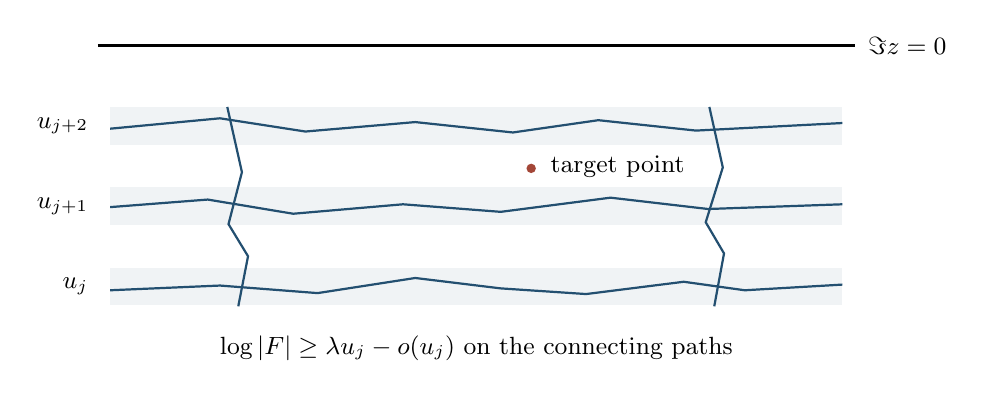
\begin{tikzpicture}[>=Stealth,x=1.55cm,y=1.2cm]
\draw[thick] (-3.1,3.05)--(3.1,3.05);
\node[font=\small,anchor=west] at (3.13,3.05) {$\Im z=0$};
\foreach \h in {.5,1.35,2.2}{
 \fill[deepblue!7] (-3,\h-.20) rectangle (3,\h+.20);
}
\draw[deepblue,thick] (-3,.46)--(-2.1,.51)--(-1.3,.43)--(-.5,.59)
 --(.2,.48)--(.9,.42)--(1.7,.55)--(2.2,.46)--(3,.52);
\draw[deepblue,thick] (-3,1.34)--(-2.2,1.42)--(-1.5,1.27)--(-.6,1.37)
 --(.2,1.29)--(1.1,1.44)--(1.9,1.32)--(3,1.37);
\draw[deepblue,thick] (-3,2.17)--(-2.1,2.28)--(-1.4,2.14)--(-.5,2.24)
 --(.3,2.13)--(1.0,2.26)--(1.8,2.15)--(3,2.23);
\draw[deepblue,thick] (-1.95,.29)--(-1.87,.82)--(-2.03,1.16)
 --(-1.92,1.71)--(-2.04,2.40);
\draw[deepblue,thick] (1.95,.29)--(2.03,.85)--(1.88,1.18)
 --(2.02,1.76)--(1.91,2.40);
\fill[warmred] (.45,1.75) circle (1.7pt);
\node[font=\small,anchor=west] at (.53,1.77) {target point};
\node[font=\small,anchor=east] at (-3.10,.50) {$u_j$};
\node[font=\small,anchor=east] at (-3.10,1.35) {$u_{j+1}$};
\node[font=\small,anchor=east] at (-3.10,2.20) {$u_{j+2}$};
\node[font=\small,align=center] at (0,-.15)
 {$\log|F|\ge\lambda u_j-o(u_j)$ on the connecting paths};
\end{tikzpicture}
\caption{The mesh in the pure first-field model. Vertical spacing is
schematic: the bands lie at logarithmic depths \(u_j+o(u_j)\).
Horizontal paths and side connectors enclose every sufficiently shallow
point of a smaller interval. Their high-modulus bounds give one common
limit \(c_*\) for the meromorphic primitive \(C_0\), where \(C_0'=F^{-2}\).
The product \(G=F(C_0-c_*)\) is holomorphic even at zeros of \(F\);
its boundary estimate therefore passes to the enclosed regions by the
maximum principle.}
\label{fig:mesh}
\end{figure}

Write \([\alpha_j,\beta_j]\) for a logarithmic-depth interval
containing the entire routed horizontal path \(\gamma_j\).  The
fixed-factor enlargements give
\(\alpha_j=u_j-s_j-O(1)\) and
\(\beta_j=u_j+s_j+O(1)\), and
\(\beta_j<\alpha_{j+1}\) for large \(j\).
Given \(z=x-\ii e^{-v}\) with \(x\in[-1,1]\) and \(v\) large,
choose \(j\) so that
\[
 \beta_j<v\le\beta_{j+1}.
\]
Then \(\gamma_j\) lies strictly below \(z\), whereas
\(\gamma_{j+2}\) lies strictly above \(z\).  The two paths
\(\sigma_j^-\) and \(\sigma_j^+\) connect across both bands and
lie strictly to the left and right of \(z\).

Choose an intersection of each side path with the lower and upper
horizontal paths, and use the corresponding path segments to form a
closed walk, in the order lower, right, upper, left.  More explicitly,
along either side path take its last lower-path hit before its first
subsequent upper-path hit; its intervening segment then joins those
two paths.  Join these endpoints along the horizontal paths.  Every
piece lies in the indicated open half-plane relative to \(z\), and
the four corner points lie in the corresponding quadrants.  This
walk has winding number one about \(z\): replace each of its pieces
by a straight segment within its open half-plane, which is convex
and avoids \(z\).  The resulting quadrilateral traverses successively
the four quadrants and has total change of argument \(2\pi\).
Equivalently, the arguments on the lower, right, upper, and left
pieces can be chosen in their respective half-plane intervals and
then joined in this order.  Self-intersections of a path or of the
walk do not affect this winding calculation.

The complementary component containing \(z\) is therefore bounded
and has boundary in this walk.  It lies compactly in the half-plane.
The maximum principle for the holomorphic function \(G\) gives its
bound there from the walk.  The upper horizontal piece has index
\(j+2\), and \(u_{j+2}=u_j+o(u_j)\), so
\eqref{model:mesh-G-bound} yields
\[
 |G(x-\ii e^{-v})|\le e^{-\lambda u_j+o(u_j)}.
\]
The same estimate is immediate if the point lies on a mesh path.
As \(v\to\infty\), the selected \(j\) tends to infinity uniformly
for \(x\in[-1,1]\).  Hence \(G\) has continuous boundary value zero
on \((-1,1)\), uniformly on compact subintervals.

Schwarz reflection across this interval extends \(G\) holomorphically
by \(\overline{G(\overline z)}\).  The extension vanishes on the
interval, so the identity theorem gives \(G\equiv0\).  On any disk
where \(F\ne0\), this says \(C_0\equiv c_*\), contradicting
\(C_0'=F^{-2}\ne0\).  The contradiction proves the Theorem.
\end{proof}

\begin{proof}[Proof of \Cref{thm:sequence-exclusion}]
Assume that a sequence in \Cref{def:prohibited-sequence} exists.
Its primary moments have a limit by
\Cref{model:moment-compactness}.  Apply
\Cref{lem:contact-dichotomy} to its logarithmic law.
The steep-contact alternative contradicts
\Cref{thm:exponential-obstruction}, as proved in
\Cref{model:steep-excluded}.  The bounded-contact
alternative gives the fields in \Cref{model:selected-fields}.
Their nonzero first field has holomorphic quotient \(F''/F\).
The limiting impact equation and parameter continuation,
\Cref{prop:pure-model,prop:model-growth}, give its uniform
upper growth.  \Cref{model:normal-epochs,prop:model-witnesses}
give common relatively dense epochs and uniform witnesses
at every horizontal center.  These are precisely the
hypotheses contradicted by \Cref{thm:mesh-contradiction}.
Both alternatives are impossible, proving the Theorem.
\end{proof}

\begin{corollary}[The critical angle budget is available]
\label{model:angle-budget-activated}
In the remaining finite-wall critical case, the angle budget
of \Cref{thm:angle-budget-reduction} and the polynomial bounds
of \Cref{cor:critical-polynomial-bounds} hold unconditionally.
In particular, for some \(\epsilon>0\),
\[
 \int_{k_0}^K\mu_f(k)^2\,\dd k\le C K^{2-\epsilon}.
\]
\end{corollary}

\begin{proof}
The sole forward assumption in the critical reduction was the
nonexistence of the sequences in
\Cref{def:prohibited-sequence}.  This is
\Cref{thm:sequence-exclusion}.  Apply the two stated
results.  Their conclusions were not used anywhere in the
proof of that theorem.
\end{proof}

\section{An odd periodic slice and its stopped geometry}
\label{sec:odd-slice}

We now work in the remaining nonisotropic case: the shape strip has finite
width \(H\), and the growth at its boundary is critical.  By
\Cref{model:angle-budget-activated}, there are constants
\(0<\rho<1\) and \(C\) such that
\begin{equation}
 \int_{k_0}^{K}\mu_f(v)^2\,\dd v\le C K^{2\rho}
 \qquad(K\ge k_0).
 \label{odd:angle-budget}
\end{equation}
We shall use this saving to control the geometry of one fixed periodic
orbit family, even when its complex continuation approaches the shape wall.
The estimates will hold up to a stopping time defined by the greatest
logarithmic shape depth visited so far. Keeping this history in the stopping rule is essential:
it permits us to use a finite collection of determinant estimates when the
sites requiring those estimates change along a path.

\subsection{The cyclic geometry and its Jacobi matrix}

Fix a sufficiently small positive parameter
\[
 t_0=\frac{2\pi}{N},\qquad N\ge3\text{ odd},
\]
inside the real analytic collar.  The integer \(N\) and the parameter \(t_0\)
are fixed throughout this section, before any limiting depth is chosen.
Set
\[
 h=h_X(t_0)=h_L(t_0),\qquad 0<h\le H,
\]
where equality of the two widths on real parameters and the upper bound
follow from the continuation results and \Cref{thm:shape-lift}.
On \(|\Im y|<h\), put
\begin{equation}
 \begin{aligned}
 s_j(y)&=\mathfrak s(y+jt_0,t_0),&
 X_j(y)&=\Gamma(s_j(y)),\\
 \psi_j(y)&=\phi(s_j(y)),&
 f_j(y)&=f(s_j(y)).
 \end{aligned}
 \label{odd:site-data}
\end{equation}
We use indices modulo \(N\), with the prescribed lifts
\(s_{j+N}=s_j+2\pi\) and \(\psi_{j+N}=\psi_j+2\pi\).
The functions \(s_j\) and \(\psi_j\) are holomorphic; the position functions
are meromorphic.

Recall
\[
 n_\theta=(\cos\theta,\sin\theta),\qquad
 e_\theta=(-\sin\theta,\cos\theta).
\]
The equations
\begin{equation}
 \theta_{j-1}+\theta_j=2\psi_j,
 \qquad \theta_{j+N}=\theta_j+2\pi
 \label{odd:angle-system}
\end{equation}
have a unique solution because \(N\) is odd.  For example, repeated
substitution expresses each \(\theta_j\) as an alternating sum of \(N\)
consecutive \(\psi\)'s plus a fixed multiple of \(\pi\).  These solutions
are holomorphic and agree, on the real collar, with the directed angles of
the billiard edges.  Consequently the identities below continue
meromorphically from that collar.  Define
\begin{equation}
 \begin{split}
 d_j^0&=\theta_j-\psi_j,\qquad
 p_j=X_j\cdot n_{\theta_j},\\
 X_{j+1}-X_j&=\ell_j e_{\theta_j},\qquad
 H_j^0=X_j\cdot n_{\psi_j}.
 \end{split}
 \label{odd:edge-data}
\end{equation}
Here and below the scalar product is the complex bilinear extension of the
Euclidean scalar product.  The chord lengths \(\ell_j\) are directed
meromorphic lengths; they are positive on the real collar.

The elementary support identities are
\begin{align}
 p_{j-1}+p_j&=2H_j^0\cos d_j^0,
 &p_j-p_{j-1}&=2(X_j\cdot e_{\psi_j})\sin d_j^0,
 \label{odd:offset-system}\\
 \dd H_j^0&=(X_j\cdot e_{\psi_j})\,\dd\psi_j,
 &\dd X_j&=c e_{\psi_j}f_j^{-2}\,\dd s_j.
 \label{odd:support-differentials}
\end{align}
Indeed, \(\theta_{j-1}=\psi_j-d_j^0\) and
\(\theta_j=\psi_j+d_j^0\), which gives the first line by addition and
subtraction.  The second line follows from
\(\Gamma'=c e_\phi f^{-2}\) and \(\phi'=f\).
Although \(X_j\) can have a pole, \(H_j^0\) is regular there.  To see the
cancellation, let \(s_0\) be a zero of \(f\).  By \Cref{lem:f-zeros},
\[
 f(s)=a(s-s_0)+O((s-s_0)^3),\qquad a\ne0.
\]
Thus \(\phi(s)-\phi(s_0)=O((s-s_0)^2)\), and the residue of \(\Gamma\)
is parallel to \(e_{\phi(s_0)}\).  Its scalar product with
\(n_{\phi(s)}\) therefore has no pole.

Oddness also makes the offset system invertible.  In fact
\[
 p_j=\sum_{m=0}^{N-1}(-1)^m H_{j-m}^0\cos d_{j-m}^0.
\]
After finding the offsets, the second equation in
\Cref{odd:offset-system} recovers the tangential component of every
\(X_j\).  In particular, if the angles and the absolute logarithms of
\(|\sin d_j^0|\) are at most \(B\), then
\begin{equation}
 \max_j|X_j|\le \exp(C(1+B))\max_j|H_j^0|.
 \label{odd:reconstruction}
\end{equation}
All constants in this section may depend on the fixed slice.

Define the symmetric matrices \(M_0\), \(\mathcal V\), and \(\mathcal H\)
by
\begin{equation}
 \langle M_0z,z\rangle
   =\sum_{j=0}^{N-1}\frac{(z_j+z_{j+1})^2}{\ell_j},\qquad
 \mathcal V_j=\frac{2f_j^3}{c\sin d_j^0},\qquad
 \mathcal H=M_0-\mathcal V,
 \label{odd:Jacobi-matrix}
\end{equation}
where \(\mathcal V\) is diagonal.  Introduce the vector
\begin{equation}
 w_j=c\sin d_j^0\,f_j^{-2}s_j'(y).
 \label{odd:w-definition}
\end{equation}

\begin{lemma}[Odd-cycle matrices]
\label{lem:odd-matrices}
The following identities hold meromorphically on the slice:
\begin{equation}
 \mathcal H w=0,\qquad
 2f_js_j'=(M_0w)_j.
 \label{odd:jacobi-angle}
\end{equation}
On the real collar, \(w_j>0\), \(\mathcal H\) is negative semidefinite,
and each of its proper principal submatrices is negative definite.
The matrix \(M_0\) is positive definite there.

More generally, let \(I\) be a proper subset of the sites and let
\(F\subseteq I^c\).  Retain the sites of \(I\) with their actual curvature,
retain the sites of \(F\) with curvature zero, and delete all other sites.
The resulting matrix
\begin{equation}
 B_{I,F}
  =(M_0)_{I\cup F,I\cup F}
    -\operatorname{diag}\bigl(\mathcal V_i\ind_{\{i\in I\}}\bigr)
 \label{odd:modified-matrix}
\end{equation}
is invertible on the real collar.  In particular its meromorphic
determinant is not identically zero.  For an empty retained set we use
determinant \(1\) and inverse norm \(0\).
\end{lemma}

\begin{proof}
First work on the real collar.  If \(\delta\mathrm{arc}_j\) is an arc-length
variation at vertex \(j\), put
\(z_j=\sin d_j^0\,\delta\mathrm{arc}_j\).  The normal projections on edge
\(j\) of the two endpoint variations are \(z_j\) and \(-z_{j+1}\).
The second variation of that edge length is therefore
\((z_j+z_{j+1})^2/\ell_j\), apart from the acceleration of the endpoint
paths.  The latter acceleration is
\(-n_{\psi_j}f_j^3/c\) per squared arc-length increment.  Pairing it with
the length gradient \(e_{\theta_{j-1}}-e_{\theta_j}\) gives
\(-2f_j^3\sin d_j^0/c\) per squared arc-length increment, or
\(-\mathcal V_j z_j^2\).  Thus \(\mathcal H\) is the length Hessian in
these variables.  Differentiation along the periodic family gives
\(\mathcal H w=0\).  Since \(\mathcal V_jw_j=2f_js_j'\), this also gives
the second identity in \Cref{odd:jacobi-angle}.  Analytic continuation
proves the meromorphic identities.

The real collar is sufficiently small that \(s_j'>0\) and
\(\sin d_j^0>0\), so \(w_j>0\).  Let \(D_w=\diag(w_j)\) and put
\(\gamma_j=w_jw_{j+1}/\ell_j>0\).  The off-diagonal entries of
\(D_w\mathcal H D_w\) are \(\gamma_j\); the identity
\(\mathcal Hw=0\) fixes its diagonal entries as
\(-\gamma_{j-1}-\gamma_j\).  Consequently
\[
 \langle D_w\mathcal H D_w z,z\rangle
   =-\sum_j\gamma_j(z_j-z_{j+1})^2.
\]
The cycle is connected.  Its only null vectors are constant, and fixing
any one coordinate to zero removes the nullspace.  This proves the two
claims concerning \(\mathcal H\).  A null vector for \(M_0\) would satisfy
\(z_{j+1}=-z_j\) for every \(j\); oddness then forces \(z=0\).

For the last assertion, arrange the retained coordinates as \(I,F\).
The truthful diagonal block is \(\mathcal H_{I,I}<0\), and the flat
diagonal block is \((M_0)_{F,F}>0\).  When both are nonempty, the Schur
complement of the flat block is
\[
 \mathcal H_{I,I}
 -(M_0)_{I,F}(M_0)_{F,F}^{-1}(M_0)_{F,I}<0.
\]
Hence the full matrix is invertible.  If one of the two blocks is empty,
one of the already proved definite-matrix statements applies.
\end{proof}

\begin{lemma}[Cofactor normalization]
\label{odd:cofactor-normalization}
Let \(A(t_0)\ne0\) be the signed area coefficient from
\Cref{eq:area-coefficient}, in the directed-edge convention used here.
Then
\begin{equation}
 w_j^2=(-1)^{N-1}\frac{A(t_0)}{N}
       \left(\prod_{i=0}^{N-1}\ell_i\right)
       \det\mathcal H_{\widehat j}.
 \label{eq:cofactor}
\end{equation}
Here \(\mathcal H_{\widehat j}\) denotes the principal matrix with site
\(j\) deleted.
\end{lemma}

\begin{proof}
On the collar let \(v_j\) be the variation obtained by differentiating
\(\mathfrak s(y+jt,t)\) with respect to \(t\), including its argument
\(jt\), and multiplying by \(c\sin d_j^0 f_j^{-2}\), at \(t=t_0\).
Periodicity gives
\[
 v_{j+N}=v_j+Nw_j.
\]
The endpoint normal differentials on edge \(j\) are
\[
 n_{\theta_j}\cdot\dd X_j=w_j\,\dd y+v_j\,\dd t,
 \qquad
 n_{\theta_j}\cdot\dd X_{j+1}
       =-w_{j+1}\,\dd y-v_{j+1}\,\dd t.
\]
Differentiating \(X_{j+1}-X_j=\ell_je_{\theta_j}\) and taking the normal
component yields
\[
 \dd\theta_j
   =\frac{(w_j+w_{j+1})\,\dd y+(v_j+v_{j+1})\,\dd t}{\ell_j}.
\]
Since
\(\dd p_j\wedge\dd\theta_j
 =(n_{\theta_j}\cdot\dd X_j)\wedge\dd\theta_j\), the area identity gives
\[
 \frac{w_jv_{j+1}-v_jw_{j+1}}{\ell_j}=A(t_0).
\]
The shift of the line phase by \((j+1/2)t\) does not alter the coefficient
of \(\dd y\wedge\dd t\).  Summing the successive differences of
\(v_j/w_j\) therefore gives
\begin{equation}
 \sum_j\frac{\ell_j}{w_jw_{j+1}}=\frac{N}{A(t_0)}.
 \label{odd:Wronskian-sum}
\end{equation}

The deleted cofactor of the negative weighted cycle Laplacian is
\[
 (-1)^{N-1}\sum_k\prod_{i\ne k}\gamma_i
   =(-1)^{N-1}\left(\prod_i\gamma_i\right)
                         \left(\sum_i\gamma_i^{-1}\right).
\]
For completeness, write the positive Laplacian as an incidence matrix,
times \(\diag(\gamma_i)\), times its transpose, and delete one vertex.
Cauchy--Binet expands the determinant over the omitted edge.  Each
remaining edge set is a path tree, whose incidence minor has determinant
\(\pm1\); this gives precisely the displayed sum.  Undoing the conjugation
by \(D_w\), and then using \Cref{odd:Wronskian-sum}, proves
\Cref{eq:cofactor} on the collar.  Both sides are meromorphic functions of
\(y\), so the identity holds throughout the slice.
\end{proof}

\subsection{Contact with the shape wall}

\begin{theorem}[Boundary contact]
\label{thm:boundary-contact}
At almost every point of either horizontal boundary of the phase strip
\(|\Im y|<h\), the functions \(s_0,\ldots,s_{N-1}\) have finite
nontangential limits, and at least one of these limits lies on
\(|\Im s|=H\).
\end{theorem}

\begin{proof}
By \Cref{thm:shape-lift}, each \(e^{\ii s_j}\) is bounded and bounded away
from zero.  The boundary limit theorem for bounded holomorphic functions
gives nontangential limits almost everywhere
\cite[Chapter~I, Theorem~5.3]{Garnett2007}.  Near a nonzero limiting
value, choose a local logarithm.  On a connected truncated approach cone
it differs from \(\ii s_j\) by one fixed integral multiple of \(2\pi\ii\).
Thus \(s_j\) itself has a finite nontangential limit.

Suppose the limiting states are all strictly inside the shape strip on a
set of positive measure.  At a point of this set we can require, in
addition, that every \(f_j\), \(\sin d_j^0\), \(\ell_j\), and
\(\det\mathcal H_{\widehat j}\) have a nonzero limit.  To justify the
requirement, first exclude limiting zeros of the \(f_j\).  Each \(f_j\)
is holomorphic on the phase strip and nonzero on the real collar.  If its
angular limit were zero on a positive-measure subset, the same boundary
uniqueness theorem used below would force \(f_j\equiv0\), a contradiction.
Thus the finite union of these exceptional sets has measure zero.
The sine and length evaluations are then regular at the interior limiting
state tuple. Exclude their zero limits next; all cofactor evaluations are
regular after those exclusions. If any one of these meromorphic functions
had limiting value zero
on a positive-measure set, Privalov's nontangential boundary uniqueness
theorem for meromorphic functions would make it identically zero
\cite[Chapter~II, p.~91]{Garnett2007}.  This is impossible by its
nondegenerate real values.  There are only finitely many functions to
exclude.  To apply the disk boundary theorems to this strip, restrict to a
compact boundary subarc of positive measure and use a conformal map to the
disk.  The map extends analytically across that subarc with nonzero
derivative, preserving null sets and nontangential approach regions.

Write \(\mathbf s=(s_0,\ldots,s_{N-1})\).  Near such a limiting tuple the
cofactor identity and \Cref{odd:w-definition} express
\[
 (s_j')^2=G_j(\mathbf s),
\]
where each \(G_j\) is analytic and nonzero.  Choose the square roots with
the signs of the actual functions on a truncated approach cone.  We obtain
a regular analytic vector equation
\(\mathbf s'=\mathbf g(\mathbf s)\).  Local solutions starting sufficiently
near the limiting tuple exist in disks of a common positive radius.
Starting at an interior point sufficiently close to the boundary, uniqueness
identifies that solution with the actual slice on their overlap.  This
continues the whole slice arc across the chosen boundary point.

It remains to explain why an extension of this single slice yields a
\emph{joint} extension, as required for \Cref{thm:no-patch}.  We give the
argument at the upper boundary.  The states
\[
 Z=(s_0,s_1)
\]
on the extended arc form a regular analytic curve, parameterized by \(y\).
All incidence angles and chords along its orbit are nondegenerate.  Thus
the local billiard return \(R\), after \(N\) reflections and subtraction
of the known \(2\pi\) shifts, is analytic near these states.  At each
reflection, this follows by solving the next incidence equation on the
regular table arc; its derivative in the next intersection coordinate is
nonzero because the sine of incidence is nonzero.  The return fixes the
extended curve, by analytic identity from below.

The determinant of its linearization at a fixed state is one.  One can
see this without choosing symplectic coordinates: successive linearized
stationarity equations in the Jacobi variables have transfer determinants
equal to ratios of consecutive off-diagonal entries.  The ratios telescope
over the cycle.  The coordinate factors converting \(\delta s_j\) to
\(c\sin d_j^0 f_j^{-2}\delta s_j\) are also periodic along the fixed orbit.
Choose local coordinates \((u,v)\) with the fixed arc given by
\((u,v)=(y,0)\).  The return consequently has the form
\begin{equation}
 R(u,v)=
 \bigl(u+\sigma(u)v+O(v^2),\ v+\tau(u)v^2+O(v^3)\bigr).
 \label{odd:return-expansion}
\end{equation}

In a lower part of this neighborhood the original joint data are known.
For
\[
 Z(y,t)=\bigl(\mathfrak s(y,t),\mathfrak s(y+t,t)\bigr),
 \qquad b=N(t-t_0),
\]
the reflection identities give
\(R(Z(y,t))=Z(y+b,t)\).  Expanding there in the coordinates just chosen,
write
\[
 u=y+O(b),\qquad v=b p_0(y)+O(b^2).
\]
The first component of the return identity at order \(b\), and its second
component at order \(b^2\), give respectively
\begin{equation}
 \sigma p_0=1,\qquad p_0'=\tau p_0^2,
 \qquad \sigma'=-\tau.
 \label{odd:return-compatibility}
\end{equation}
These identities continue along the extended arc.  By moving the boundary
point slightly within this arc if necessary, take a smaller neighborhood
where \(\sigma\ne0\), and set \(p_0=1/\sigma\).

For small nonzero \(b\) with \(|\Im b|\ge |b|/3\), the return and its
inverse continue the joint states upwards in steps \(\pm b\).  Here are
the relevant uniform estimates.  In the coordinates \((u,p)=(u,v/b)\),
\Cref{odd:return-expansion} reads
\[
 (u,p)\longmapsto(u,p)
       +b\bigl(\sigma(u)p,\tau(u)p^2\bigr)+O(b^2)
\]
on fixed compact subsets; the inverse has the negative first increment.
The analytic differential equation with that vector field has the regular
solution \((u,p)=(y,p_0(y))\), by
\Cref{odd:return-compatibility}.  Choose the arc neighborhood and the
height to be crossed sufficiently small.  The steepness condition keeps
all the slanted paths from the lower starting slab inside that neighborhood.
There are \(O(1/|b|)\) steps; each has error \(O(|b|^2)\) and stability
factor at most \(1+C|b|\).  The continued states therefore stay within
\(O(|b|)\) of this regular solution.  All shape coordinates remain strictly
inside the shape strip.

All intermediate site coordinates are recovered by the regular analytic
billiard steps along the orbit.  Thus their continuations agree with the
original \(s_j\)'s wherever the latter were already defined.

Use locally constant numbers of backward steps to place initial states
in the lower slab.  On overlaps, the exact return identity in that slab
and uniqueness of each forward step identify the constructions.  They
give joint holomorphic germs in the steep sectors, attached by vertical
continuation to the lower data.

Finally choose a small \(\eta>0\), then a much smaller \(r>0\), and use
the analytic disks
\begin{equation}
 t=t_0+r\zeta,\qquad
 y=x_*+\ii\varsigma-\ii\eta\zeta^2+w,
 \qquad |\zeta|\le1,
 \label{odd:contact-disks}
\end{equation}
as \(\varsigma\) rises from \(h-2\eta\) to \(h\); \(w\) varies in a
sufficiently small complex disk.  On the boundary arcs where \(\zeta\)
is near the real axis, the phase point is a fixed amount below the wall.
For small \(r\), these arcs lie in the original joint tube, by lower
semicontinuity of the width.  On the remaining arcs the parameter is in
a fixed steep sector, so the preceding continuation applies.  The collar
germs agree because both are vertical continuations of the lower data.
The full disks are initially inside known data.  Holomorphic product
continuation, as in \Cref{lem:meromorphic-hartogs}, fills them as the center
is raised.  Equivalently, pull the germs back to a collar of the unit circle
and a complex neighborhood of the center path: the negative Cauchy moments
vanish in the initial open part and hence throughout that connected
neighborhood. More explicitly, combine \(x_*+\ii\varsigma+w\) into
one complex center variable \(a\). The map
\((a,\zeta)\mapsto(a-\ii\eta\zeta^2,t_0+r\zeta)\)
has Jacobian determinant \(r\ne0\), so the filling supplies a joint
neighborhood in \((y,t)\).

The maximum principle preserves \(|\Im s_j|<H\) on the filled disks.
Composition with \(\Gamma\) gives a joint meromorphic patch for \(X\) at
\((x_*+\ii h,t_0)\), agreeing with the original tube below the wall.
This contradicts \Cref{thm:no-patch}, which applies also to the rational
parameter \(t_0\).  The lower boundary is treated in the same way, or by
real symmetry.  The supposed positive-measure set therefore cannot exist.
\end{proof}

\subsection{Brownian motion, history levels, and fixed stopping rules}

We use the standard conformal time-change, optional-stopping, and
martingale maximal theorems for Brownian motion; see
\cite[Chapters~II, IV and V]{RevuzYor1999}. Their applications, including the stopping cuts,
are specified below.
Let \(y_u\) be planar Brownian motion, started with \(y_0\) uniform on one
real period, and let \(\zeta\) be its first exit from \(|\Im y|<h\).
All functions are evaluated on the real lift of this path.  Put
\begin{equation}
 \begin{aligned}
 \delta_j(u)&=H-|\Im s_j(y_u)|,&
 k_j(u)&=-\log\delta_j(u),&
 K_j(u)&=\max_{0\le v\le u}k_j(v),\\
 r_y(u)&=h-|\Im y_u|,&
 n_y(u)&=-\log r_y(u),&
 \tau_L&=\inf\{u:\max_jK_j(u)=L\}.
 \end{aligned}
 \label{odd:stopping-data}
\end{equation}
For sufficiently large \(L\), \(\tau_L<\zeta\) almost surely.  Indeed the
bounded functions \(e^{\ii s_j}\) are Poisson integrals of their almost
everywhere boundary values.  This follows first on narrower strips and
then on the whole strip by dominated convergence.  Along Brownian motion
they are the conditional-expectation martingales of their terminal boundary
values.  Announcing the exit by exits from narrower strips shows that their
limits at Brownian exit are those terminal values.  The exit distribution
is absolutely continuous on the horizontal boundary, so
\Cref{thm:boundary-contact} makes at least one \(\delta_j\) tend to zero.
Continuity then gives every sufficiently large history level before exit.

The isolated zeros and poles of the meromorphic slice functions are polar
for planar Brownian motion and are almost surely avoided.  All statements
involving them can first be stopped on compact subsets avoiding these
points, followed by an exhaustion.  In what follows, ``with probability
tending to one through \(\tau_L\)'' means that one event of probability
\(1-o(1)\) supports the stated bounds simultaneously at every time
\(0\le u\le\tau_L\) and at every site.

\begin{lemma}[Shape time change and its consequences]
\label{odd:time-change}
Each process \(s_j(y_u)\), before phase exit, is a Brownian motion in the
shape strip under the scalar time change
\[
 Q_j(u)=\int_0^u|s_j'(y_v)|^2\,\dd v,
\]
possibly stopped before shape exit.  Its initial horizontal law has a
density bounded by a fixed constant relative to uniform measure modulo
\(2\pi\).  In particular:
\begin{enumerate}[label=\textup{(\roman*)}]
 \item The expected occupation of any nonnegative periodic shape
 observable, integrated against \(\dd Q_j\), is bounded by a fixed
 constant times its ordinary shape-strip occupation from a uniform real
 start.  The total shape clocks have bounded expectation.  Moreover,
 \begin{equation}
  \E\int_0^{\tau_L}
       \ind_{\{k_j(u)\le K\}}|f_j(y_u)s_j'(y_u)|^2\,\dd u
       \le C(1+K)^{2\rho}
  \label{odd:angle-clock}
 \end{equation}
 for large \(K\).
 \item At the first hit of a deterministic shape-depth row, the
 subprobability law of the hit is dominated by a fixed constant times the
 corresponding law for ordinary shape Brownian motion from a uniform real
 start.  In particular that ordinary horizontal law is uniform.
 \item After a first hit of shape depth \(\delta\), the remaining shape
 clock before any later phase stop has tail at most
 \begin{equation}
  C\min\left(1,\frac{\delta}{\sqrt T}\right)
  \label{odd:remaining-shape-clock}
 \end{equation}
 at clock time \(T>0\).  This estimate also holds conditionally at that
 hit whenever it occurs.
 \item For a sufficiently large fixed \(C\), with probability tending
 to one through \(\tau_L\),
 \begin{equation}
  k_j(u)\ge K_j(u)-C\log L\qquad\text{for every }j.
  \label{odd:retreat}
 \end{equation}
\end{enumerate}
\end{lemma}

\begin{proof}
The real and imaginary parts of a holomorphic function of planar Brownian
motion are local martingales.  The Cauchy--Riemann equations give equal
quadratic variations \(\dd Q_j\) and zero mutual quadratic covariation.
The Brownian time-change theorem therefore applies.  To use it up to a
given interior phase stop, append independent Brownian increments in
intrinsic time after that stop.  The extension cannot have exited the
shape strip before the part of the path already used, because all those
states lie in the strip.  Approximation by compact interior stops proves
the same domination for nonnegative occupations over the whole phase
interval.

On the real collar \(y\mapsto s_j(y)\) is an increasing analytic circle
diffeomorphism whose derivative is bounded above and below.  This proves
the initial-density assertion.  Under a uniform real start, the periodic
shape-strip Green weight is a constant times
\(\delta=H-|\Im s|\).  It has finite integral, proving the total-clock
claim.  At either wall, the contribution of \(|f|^2\) up to log depth
\(K\) is bounded by a constant times
\[
 \int_{e^{-K}}^{\delta_*}\delta\,\E|f|^2\,\dd\delta
   =\int_{k_*}^{K}\delta^2\E|f|^2\,\dd k
   =\int_{k_*}^{K}\mu_f(k)^2\,\dd k.
\]
The fixed interior region has bounded contribution.  Now use
\Cref{odd:angle-budget}.  Domination of first-hit laws follows from the
same Brownian extension; if the original path never reaches the row,
it contributes no mass.

Starting at distance \(\delta\) from one horizontal wall, the exit time
from the strip is no greater than the first time the vertical Brownian
coordinate hits that particular wall.  The one-dimensional reflection
principle bounds survival to time \(T\) by
\(C\min(1,\delta/\sqrt T)\).  Applying this after the hit, with the
strong Markov property in intrinsic time, proves (iii).

For (iv), at the first hit of each integer level \(m\), the probability
of reaching depth \(R e^{-m}\) before hitting the adjacent wall is at
most \(1/R\), by the linear one-dimensional hitting probability.  Take
\(R\) a sufficiently large fixed power of \(L\), and sum over the
\(O(L)\) integer levels up to \(L\), and the fixed number of sites.
If a retreat larger than \(C\log L\) occurred, it would contain one of
these integer-level retreats, with an immaterial factor from rounding.
The union probability tends to zero.
\end{proof}

We record explicitly the two localization principles used below.

\begin{lemma}[Logarithmic deficit at a stopping cut]
\label{odd:log-deficit}
Let \(g\) be a nontrivial meromorphic slice function, with
\(\log|g(y_0)|\ge-C_0\) on the real starting row.  Suppose
\(\log|g(y_u)|\le B_0\), where \(B_0\ge1\), up to a specified stopping
cut \(T\).  Then
\begin{equation}
 \Prob\left\{\inf_{u\le T}\log|g(y_u)|<-B_1\right\}
     \le \frac{B_0+C_0}{B_0+B_1}
     \le\frac{C(1+B_0)}{1+B_1}
 \label{odd:log-deficit-probability}
\end{equation}
for \(B_1\ge1\).  Earlier bounds may be incorporated by stopping at their
first failure; their failure probabilities are then added separately.
\end{lemma}

\begin{proof}
Away from the polar zero and pole set, \(\log|g(y_u)|\) is a continuous
local martingale.  Before the indicated cut,
\(B_0-\log|g(y_u)|\) is nonnegative, hence is a supermartingale after
localization.  Stop additionally at its first hit of \(B_0+B_1\).
The supermartingale inequality gives the first bound.  Exhaustion removes
the auxiliary compact localizations.
\end{proof}

For an analytic differential integrated after a stopping time, we shall
likewise apply the maximal inequality only after a quadratic-time cut.
More precisely, if its scalar quadratic time is at most a deterministic
\(B\) on some collection of paths, stop the integral at quadratic time
\(2B\) before estimating its maximum.  The resulting second-moment bound
is \(O(B)\).  It applies to the original integral on those paths, without
conditioning on the collection of paths.  This remains true when the
integrand is masked by adapted status indicators, using their predictable
versions.  All ensuing probability estimates use these cuts.

Put
\begin{equation}
 a_j=\log|f_j|,
 \qquad
 \mathcal G(u)=\max_j\left(
  |\psi_j|+\log(1+|X_j|)
       +|\log|\sin d_j^0||+|\log|\ell_j||\right)(y_u).
 \label{odd:geometry-size}
\end{equation}
By \Cref{cor:critical-polynomial-bounds}, everywhere before the relevant
history stop,
\begin{equation}
 a_j\le k_j^++C\log(2+k_j^+)+C,
 \qquad k_j^+=\max(k_j,0).
 \label{odd:amplitude-upper}
\end{equation}

\begin{lemma}[A finite family of modified inverse estimates]
\label{odd:modified-inverses}
Let \(V\ge U\ge1\) be deterministic.  For each fixed proper truthful set
\(I\) and flat set \(F\subseteq I^c\), stop at \(\tau_L\), at the first
failure of \(\mathcal G\le U\), or at the first time an \(I\)-history
exceeds \(U\), whichever comes first.  Except on an event of probability
at most
\begin{equation}
 \frac{C(1+U)}{1+V},
 \label{odd:inverse-failure}
\end{equation}
the bound
\begin{equation}
 \|B_{I,F}^{-1}\|\le\exp(CV)
 \label{odd:inverse-bound}
\end{equation}
holds throughout this stopped interval.  The constant is uniform over
the finitely many choices of \(I,F\).  Thus one may secure all these
bounds by a finite union, and subsequently choose \(I,F\) as functions of
the current state before the common geometry cut, whenever their selected
history caps hold.
\end{lemma}

\begin{proof}
On the stopped interval, \Cref{odd:amplitude-upper} bounds \(a_i\) by
\(C(1+U)\) for \(i\in I\).  The geometry cap bounds the reciprocal
lengths, the reciprocal incidence sines, and the angles.  Hence every
entry, determinant, and cofactor of \(B_{I,F}\) has modulus at most
\(\exp(C(1+U))\).  There is no amplitude bound required at flat or deleted
sites: their curvature terms do not appear.  By \Cref{lem:odd-matrices},
the determinant has a positive minimum in modulus on the compact real
starting period.  Apply \Cref{odd:log-deficit} to that determinant with
upper bound \(C(1+U)\) and lower-log threshold \(-V\).  The adjugate
formula gives \Cref{odd:inverse-bound} outside the resulting exceptional
event.  Empty matrices require no estimate.

There are at most \(3^N\) choices.  Each matrix is defined and estimated
from the original real start, with its own fixed stopping rule.  If at
a later time all the histories selected by that matrix are at most \(U\),
none of them has crossed its cap previously.  Thus the estimate already
secured for that fixed candidate is still valid as long as the common
geometry cut has not occurred.  This is the reason for
using history levels rather than current depths.  No estimate is restarted
when the current selection changes.
\end{proof}

\subsection{An initial bound below linear order}

\begin{lemma}[Initial stopped geometry]
\label{odd:initial-geometry}
There is a fixed \(\sigma<1\) such that
\[
 \mathcal G(u)\le L^\sigma\qquad(0\le u\le\tau_L)
\]
with probability tending to one as \(L\to\infty\).
\end{lemma}

\begin{proof}
The angle differential is \(\dd\psi_j=f_j\,\dd s_j\).  Up to \(\tau_L\)
all current log depths are at most \(L\), so
\Cref{odd:angle-clock} and the maximal inequality bound all angles by
\(L^{\rho+\eps}\) with probability tending to one, for each fixed
\(\eps>0\).  The linear equations \eqref{odd:angle-system} give the same
bound for \(\theta_j,d_j^0\).  They imply an upper bound of this order for
\(\log|\sin d_j^0|\).  The sine has a positive minimum on the real
starting collar.  Applying \Cref{odd:log-deficit} with a slightly larger
power gives, for some fixed \(\rho<\rho'<1\), simultaneous angle and sine
cost at most
\[
 r_*=L^{\rho'}.
\]
We stop at the first failure of these bounds for the estimates that follow,
and add the already vanishing failure probability at the end.

Choose
\[
 G=L^\gamma,\qquad \frac{1+\rho'}2<\gamma<1,
\]
and a small fixed \(b>0\).  At each site use two statuses, initially
moderate.  Switch from moderate to tiny at a downcrossing of
\(a_j=-2bG\), and switch back at an upcrossing of \(a_j=-bG\).
The hysteresis gap is \(bG\).  By \Cref{odd:amplitude-upper},
\(CL-a_j\) is a nonnegative local martingale, hence a supermartingale,
up to \(\tau_L\) and the preceding cuts. Its upcrossing levels are
\(CL+bG\) and \(CL+2bG\). The upcrossing inequality, and alternation
of the two switch directions, give an expected number of switches
\(O(L/G)\). One can also obtain this
bound by holding supermartingale increments during attempted passages
between the two levels: each completed passage earns \(bG\), while an
unfinished passage has possible loss bounded by \(CL+2bG\).
Thus, for any sufficiently small fixed \(\eps_1>0\), the total number of
switches over the fixed number of sites is at most
\begin{equation}
 L^{1+\eps_1}/G
 \label{odd:switch-count}
\end{equation}
with probability tending to one.

Let
\[
 \mathcal R(u)=1+\sup_{0\le v\le u,\,j}|X_j(y_v)|.
\]
During a moderate interval, \(a_j\ge-2bG\).  From
\Cref{odd:support-differentials}, the coefficient of \(\dd s_j\) in
\(\dd X_j\) has modulus at most \(e^{5bG}\), for large \(L\), because
\(r_*=o(G)\).  During a tiny interval, \(a_j\le-bG\), and the coefficient
of \(\dd s_j\) in \(\mathcal R^{-1}\dd H_j^0\) has modulus at most
\(e^{-bG/2}\).  The latter estimate uses
\[
 \mathcal R^{-1}|X_j\cdot e_{\psi_j}|\,|f_j|
       \le \exp(Cr_*-bG).
\]
Mask these two differentials by their corresponding status indicators.
The total expected shape clocks are bounded by
\Cref{odd:time-change}.  The maximal inequality, with the cuts described
above, shows that the cumulative moderate-position integrals and
tiny-support integrals have respective suprema at most
\begin{equation}
 e^{6bG},\qquad e^{-bG/3}
 \label{odd:masked-integrals}
\end{equation}
with probability tending to one.

On a tiny interval, write \(\dd H_j^0=\mathcal R\,\dd M_j\), where the
appropriate masked martingale \(M_j\) is bounded as in
\Cref{odd:masked-integrals}.  Integration by parts against the continuous
increasing function \(\mathcal R\) bounds the support increment on any
such interval by
\(C e^{-bG/3}\mathcal R\) at its endpoint.  For example, after subtracting
the starting value of \(M_j\), both the endpoint term and the integral
against \(\dd\mathcal R\) are bounded by that quantity.

Between successive switches of the joint status vector, a moderate site's
position differs from its starting position by at most \(2e^{6bG}\), and
a tiny site's support has the preceding increment bound.  If
\(\mathcal R_{\rm start}\) is the running maximum at the start of such
an interval, every support during it is therefore at most
\begin{equation}
 e^{Cr_*}\bigl(\mathcal R_{\rm start}+C e^{6bG}\bigr)
       +C e^{-bG/3}\mathcal R.
 \label{odd:support-interval-bound}
\end{equation}
Use \Cref{odd:reconstruction} and absorb the last term; its coefficient
after reconstruction tends to zero because \(r_*=o(G)\).  Each interval
then multiplies the maximum of its starting bound and \(C e^{6bG}\) by
at most \(e^{Cr_*}\).  By \Cref{odd:switch-count}, its accumulated
logarithmic cost is at most
\[
 C r_*L^{1+\eps_1}/G=o(G),
\]
provided \(\eps_1\) is small enough that
\(2\gamma>1+\rho'+\eps_1\).  Hence \(\log\mathcal R\le C G\) with
probability tending to one.

The identity \(\ell_j=(X_{j+1}-X_j)\cdot e_{\theta_j}\) now gives upper
logarithmic length bounds of the same order.  Apply
\Cref{odd:log-deficit} to each nonzero length, allowing a further small
increase of the exponent, to obtain lower logarithmic bounds.  Choose a
fixed \(\sigma\) strictly between all these exponents and \(1\).
Constants are then absorbed by \(L^\sigma\) for large \(L\), proving the
claim.  Each previous good bound was enforced by its first-failure cut;
only the sum of their vanishing exceptional probabilities has been added.
\end{proof}

\begin{lemma}[Phase depth and phase clock]
\label{odd:phase-clock}
For some fixed \(C\), with probability tending to one through \(\tau_L\),
\begin{equation}
 n_y(u)\le CL,\qquad
 \int_0^{\tau_L}r_y(u)^{-2}\,\dd u\le L^C.
 \label{odd:phase-clock-bounds}
\end{equation}
\end{lemma}

\begin{proof}
Apply \Cref{odd:initial-geometry} through \(\tau_{2L}\).  The entries of
\(\mathcal H\) have upper logarithmic size \(O(L)\), by
\Cref{odd:amplitude-upper}; the incidence sines and lengths have only
sublinear logarithmic cost.  The cofactor formula
\Cref{eq:cofactor} consequently gives
\begin{equation}
 |w_j|+|s_j'|\le e^{C_1L}
 \label{odd:rough-derivative-bound}
\end{equation}
through that stop on the good paths.  The second bound follows from
\Cref{odd:w-definition}, using the amplitude upper bound again.

Let \(T\) be the first phase depth \(r_y=e^{-C_2L}\), with \(C_2\) fixed
and sufficiently large.  By the one-dimensional hitting estimate, after
\(T\) the remaining phase time is at most \(e^{-C_2L}\), except with
probability at most \(C e^{-C_2L/2}\).  Suppose \(T<\tau_L\).  At time
\(T\), all shape depths are at least \(e^{-L}\), whereas at
\(\tau_{2L}\) one of them is \(e^{-2L}\).  On the good derivative paths,
the quadratic time of each shape increment from \(T\) to
\(\tau_{2L}\) is bounded by
\(e^{2C_1L-C_2L}\).  Enforce this by the derivative cut and by a physical
time cut of \(e^{-C_2L}\) after \(T\).  The maximal inequality then shows
that, for sufficiently large \(C_2\), all these increments are
\(o(e^{-L})\) with probability tending to one.  This contradicts the
required change of one imaginary part by at least
\(e^{-L}-e^{-2L}\).  Thus \(T<\tau_L\) has probability tending to zero,
which proves the first bound.

Under the uniform real start, the phase-strip Green weight at a wall is
proportional to \(r_y\).  Therefore
\[
 \E\int_0^\zeta
    \ind_{\{r_y\ge e^{-C_2L}\}}r_y^{-2}\,\dd u
       \le C(1+L).
\]
On the already established good depth event, the integral through
\(\tau_L\) is part of this truncated occupation.  Markov's inequality,
for example at threshold \(L^2\), gives a polynomial bound with
probability tending to one.  Increasing the single constant \(C\) if
necessary yields \Cref{odd:phase-clock-bounds}.
\end{proof}

\subsection{Improvement to every positive power}

\begin{theorem}[Stopped geometry at every power]
\label{thm:stopped-geometry}
For every fixed \(\sigma>0\), with probability tending to one as
\(L\to\infty\),
\begin{equation}
 \mathcal G(u)\le L^\sigma\qquad(0\le u\le\tau_L).
 \label{odd:all-power-geometry}
\end{equation}
The phase-depth and phase-clock bounds of \Cref{odd:phase-clock} hold
simultaneously.  All estimates concern the same fixed odd slice.
\end{theorem}

\begin{proof}
It suffices to improve an exponent \(0<\sigma<1\) already known to work.
Choose a small fixed \(\eps>0\) with \(\sigma+\eps<1\), and put
\[
 H_0=L^{\sigma+\eps}.
\]
The old estimate, applied at level \(H_0\), gives geometry at most
\(H_0^\sigma\) through \(\tau_{H_0}\), with probability tending to one.
We shall show that, after this time, angles and supports change by amounts
exponentially smaller than this improved initial scale.

Choose a sufficiently small fixed \(\eta>0\), and a finite family of
disjoint intervals \((\xi_m,\xi_m+\eta)\) inside
\((\sigma+\eps/3,\sigma+\eps)\), with more than \(N\) members.  At every
time after \(\tau_{H_0}\), at least one history is \(\ge H_0\).  There is
one choice \(\xi=\xi_m\) for which the corresponding power interval
\((L^\xi,L^{\xi+\eta})\) contains none of the \(N\) history levels.
For that choice, partition the sites as
\[
 I=\{j:K_j\le L^\xi\},\qquad
 I^c=\{j:K_j\ge H_*\},\qquad H_*=L^{\xi+\eta}.
\]
Endpoint equalities can be assigned to their respective sets; they do not
affect any estimate.  The set \(I\) is proper because one history is
\(\ge H_0\).  By \Cref{odd:retreat}, every deep site's current log depth
satisfies \(k_j\ge H_*/2\), on an event of probability tending to one.

We secure all matrix inverses before making any state-dependent selection.
For each fixed \(\xi_m\), proper set \(I\), and flat subset \(F\subseteq
I^c\), use \Cref{odd:modified-inverses} with, for instance,
\[
 U=L^{\xi_m+\eta/4},\qquad V=L^{\xi_m+\eta/2}.
\]
The old geometry cap \(L^\sigma\) and the selected truthful history cap
\(L^{\xi_m}\) both lie below \(U\) for large \(L\).  The failure probability
is \(O(L^{-\eta/4})\) for each candidate.  The number of candidates is
fixed, so outside one event of probability tending to zero, all required
inverses have norm
\begin{equation}
 \|B_{I,F}^{-1}\|\le
       \exp\bigl(C L^{\xi+\eta/2}\bigr)
       =\exp(o(H_*)).
 \label{odd:gap-inverse}
\end{equation}
These bounds hold whenever the corresponding histories are below their
caps, regardless of how often the empty gap and the flat subset change.

Set
\[
 z_j=r_y w_j.
\]
Schwarz--Pick, transported from the disk by conformal maps of the two
strips, gives \(r_y|s_j'|\le C\delta_j\)
\cite[Chapter~I, Lemma~1.2]{Garnett2007}; the strip hyperbolic densities
are comparable with reciprocal boundary distance.  Hence
\Cref{odd:w-definition} and the old geometry bound imply
\begin{equation}
 \log|z_j|+2a_j+k_j\le C L^\sigma,
 \label{odd:Schwarz-suppression}
\end{equation}
with the usual interpretation when \(z_j=0\).
Fix a sufficiently small positive constant \(c_1\).  Among the deep sites
retain as flat exactly those for which
\[
 |z_j|>e^{-c_1H_*};
\]
call this set \(F\), and delete the other deep sites.  At a retained deep
site, \Cref{odd:Schwarz-suppression} and \(k_j\ge H_*/2\) imply
\(a_j<-c_2H_*\) for a fixed \(c_2>0\), since \(L^\sigma=o(H_*)\).
Consequently its actual curvature term obeys
\[
 |\mathcal V_j|\le e^{-c_3H_*}
\]
for another fixed positive constant.  Every deleted coordinate already
has modulus at most \(e^{-c_1H_*}\).

Apply the equation \((M_0-\mathcal V)z=0\) to the retained coordinates
\(I\cup F\).  Its left matrix is \(B_{I,F}\) minus the tiny curvature
diagonal on \(F\); its right side is the coupling to the deleted
coordinates.  Entries of \(M_0\) cost at most \(e^{CL^\sigma}\).
By \Cref{odd:gap-inverse}, the tiny diagonal is absorbable, and the
right side gives
\begin{equation}
 \max_j|z_j|\le e^{-c_4H_*}
 \label{odd:all-sites-suppressed}
\end{equation}
for a fixed \(c_4>0\), uniformly over all the finite choices.  The same
argument includes an empty deleted set, in which case the retained
homogeneous system has only the zero solution.

The important consequence is suppression at \emph{every} site, including
the shallow ones.  From \Cref{odd:jacobi-angle},
\begin{equation}
 2r_y\partial_y\psi_j
      =\mathcal V_j z_j=(M_0z)_j.
 \label{odd:all-angle-suppression}
\end{equation}
Since \(H_*\ge L^{\sigma+\eps/3}\), the right side has modulus at most
\(\exp(-cL^{\sigma+\eps/3})\), with a fixed \(c>0\), after decreasing
that constant if necessary.  The phase-clock bound now makes the quadratic
time of each angle increment after \(\tau_{H_0}\) exponentially small.
Cut at that deterministic quadratic-time bound and apply the maximal
inequality.  We obtain, with probability tending to one,
\begin{equation}
 \sup_{\tau_{H_0}\le u\le\tau_L}
   |\psi_j(y_u)-\psi_j(y_{\tau_{H_0}})|
        \le \exp(-c' L^{\sigma+\eps/3}).
 \label{odd:late-angle-increments}
\end{equation}
All choices of history gaps and flat sets have disappeared from this
martingale statement: they were used only to prove the uniform pointwise
differential bound on the fixed good event.

The angles at \(\tau_{H_0}\) have size at most \(H_0^\sigma\).
Their incidence sines have modulus at least \(e^{-H_0^\sigma}\).
The absolute change of each sine is at most the angle change times
\(\exp(CL^\sigma)\), using the old angle bound along the interval.
By \Cref{odd:late-angle-increments}, this is negligible relative to its
improved initial lower bound.  Thus the angles and both logarithmic sine
bounds keep cost \(O(H_0^\sigma)\) throughout the late interval.

The supports obey the same improvement.  By
\Cref{odd:support-differentials},
\[
 \mathcal R^{-1}\dd H_j^0
    =\mathcal R^{-1}(X_j\cdot e_{\psi_j})\,\dd\psi_j.
\]
Its coefficient relative to the angle differential has modulus at most
\(e^{CL^\sigma}\) by the old bound.  Combining
\Cref{odd:all-angle-suppression} with the phase clock shows that the
martingale integral of this differential over the single late interval
has exponentially small supremum.  Integration by parts against the
increasing \(\mathcal R\), as in the initial geometry argument, gives
\[
 |H_j^0(y_u)-H_j^0(y_{\tau_{H_0}})|
    \le e^{-c''L^{\sigma+\eps/3}}\mathcal R(u)
\]
on a further event of probability tending to one.  Reconstruct positions
with \Cref{odd:reconstruction}, now using the improved angle and sine cost
\(O(H_0^\sigma)\).  The initial positions and supports have this same
logarithmic cost.  The coefficient of \(\mathcal R(u)\) in the last
display remains exponentially small after reconstruction and is absorbed.
It follows that
\[
 \log\mathcal R(u)\le C H_0^\sigma
       =C L^{\sigma(\sigma+\eps)}
       \qquad(u\le\tau_L)
\]
with probability tending to one.

The length upper logs have the same improved bound.  For their lower logs,
cut at the first failure of this upper bound. Choose \(\eps\) small
enough that
\[
\sigma(\sigma+\eps)<\frac{\sigma+\sigma^2}{2}<\sigma.
\]
Choose a power strictly between the first two quantities as the lower
threshold in \Cref{odd:log-deficit}; its failure probability tends to zero.
All fixed constants and all needed lower-log slack are then absorbed by
the new exponent \((\sigma+\sigma^2)/2\).  This proves an improvement of
the old assertion.

Starting with \Cref{odd:initial-geometry}, iterate this improvement a
finite number of times.  The sequence generated by
\(\sigma\mapsto(\sigma+\sigma^2)/2\), starting below one, decreases to
zero.  Given any desired positive exponent, choose the number of iterations
in advance, independently of \(L\).  There are then only finitely many
exceptional events to discard, each with probability tending to zero.
This proves \Cref{odd:all-power-geometry};
\Cref{odd:phase-clock} supplies the simultaneous phase estimates.
\end{proof}

\section{Sign tests and the last moving site}
\label{sign:section}

We finish the exclusion of a finite critical wall.
\Cref{model:angle-budget-activated} supplies both the angle budget and
the polynomial bounds of \Cref{cor:critical-polynomial-bounds}.
In particular, with
\(d_k=e^{-k}\) and horizontal means normalized to have mass one,
\begin{equation}\label{sign:polynomial-input}
 \mu(k)\le C(1+k),\qquad
 d_k\sup_x\bigl(|f|+\sqrt{|q|}\bigr)
       (x+\ii(H-d_k))\le C(1+k)^2.
\end{equation}
Real symmetry gives the same estimates at the lower wall.  All constants
below may depend on the fixed billiard and on fixed tile enlargements.
They never depend on the large parameters \(K\) and \(L\).

Fix throughout
\begin{equation}\label{sign:alpha}
 \alpha=\frac1{100}.
\end{equation}
The purpose of the first part of the section is to find a deterministic
shape row on which almost every point has either very small or very large
\(|f|\).  Both alternatives suppress the motion of that site in the odd
Jacobi system, but by different identities.  The final argument applies
this suppression to the last site to cross the tested row.

\subsection{A discrete occupation estimate}

We first isolate the probabilistic estimate needed when the row moments
are small.  It does not require a bound on the starting value of the
submartingale.

\begin{lemma}[Discrete Tanaka estimate]\label{lem:discrete-tanaka}
Let \((X_m)_{0\le m\le M}\) be an integrable real submartingale, and suppose
\[
 V=\sum_{m=0}^{M-1}\E(X_{m+1}-X_m)^2<\infty.
\]
For \(0<h<R\), put
\[
 \mathcal C_h=
 \sum_{m=0}^{M-1}\E\left[
 \ind_{\{|X_m|\le h\}}
 \min\{(X_{m+1}-X_m)^2,h^2\}\right].
\]
There is an absolute constant \(C\) such that
\begin{equation}\label{sign:tanaka-bound}
 \mathcal C_h\le
 C h(h+R+\sqrt V)
 +C M h^2\min\left\{1,\frac{V}{(R-h)^2}\right\}.
\end{equation}
\end{lemma}

\begin{proof}
Use the increasing convex function
\[
 \Phi(x)=\sqrt{h^2+x^2}+x.
\]
Its derivative is between \(0\) and \(2\), it is nonnegative, and
\(\Phi(x)\le h+2x^+\).  Moreover,
\(\Phi''(x)\ge c/h\) on \([-2h,2h]\).  Integrating this second derivative
along the first \(\min\{|y-x|,h\}\) of the segment from \(x\) to \(y\)
proves
\begin{equation}\label{sign:ramp-remainder}
 \Phi(y)-\Phi(x)-\Phi'(x)(y-x)
 \ge \frac c h\ind_{\{|x|\le h\}}\min\{(y-x)^2,h^2\}.
\end{equation}
This includes a displacement that leaves \([-2h,2h]\), because the
remaining convex remainder is nonnegative.

Let \(T\) be the first index at which \(X_m>R\), capped at \(M\).
If \(X_0>R\), set \(T=0\).  Sum \eqref{sign:ramp-remainder} only on
\(m<T\).  Conditional expectation removes the linear term with the correct
sign, since \(\Phi'\ge0\) and the conditional drift is nonnegative.
The resulting sum is at most
\(C h\E[\Phi(X_T)-\Phi(X_0)]\).  Paths starting above \(R\) contribute
zero.  On the others the terminal positive part is at most
\[
 R+\max_{m<M}|X_{m+1}-X_m|,
\]
including the crossing increment.  Cauchy--Schwarz therefore bounds the
pre-\(T\) cost by \(C h(h+R+\sqrt V)\).

Write
\[
 b_m=\E[X_{m+1}-X_m\mid\mathcal F_m]\ge0,\qquad
 Z_n=\sum_{m<n}\ind_{\{T\le m\}}
       (X_{m+1}-X_m-b_m).
\]
This is a square-integrable martingale starting at zero, with terminal
second moment at most \(V\).  If a chain which starts above \(R\), or
crosses \(R\), subsequently returns to \([-h,h]\), then
\(\sup_n|Z_n|\ge R-h\); accumulated drift cannot assist this downward
move.  The martingale maximal inequality bounds the probability of any
such return by \(C\min\{1,V/(R-h)^2\}\).  After \(T\), the entire cost is
at most \(Mh^2\) on that event.  Adding the two estimates proves
\eqref{sign:tanaka-bound}.  In particular, no conditional estimate given
the crossing event has been used.
\end{proof}

\subsection{The large-moment alternative}

\begin{lemma}\label{sign:large-moment}
Suppose that, along a sequence \(K\to\infty\), some
\(j\in[0.9K,2.1K]\) satisfies \(\mu(j)\ge K^\alpha\).  There is a
deterministic \(k\in[0.8K,2.2K]\) for which
\begin{equation}\label{sign:row-small-exception}
 \frac1{2\pi}\left|\left\{x\in[0,2\pi]:
 \left|\log|f(x+\ii(H-e^{-k}))|\right|
           \le K^{\alpha/2}\right\}\right|\longrightarrow0.
\end{equation}
\end{lemma}

\begin{proof}
Choose a small fixed \(c>0\), with \(c<1/4\), and maximize
\(\mu(l)e^{-c|l-j|}\) over \(l\ge k_0\).  The maximum exists by
\eqref{sign:polynomial-input}.  A maximizer \(k\) satisfies
\[
 |k-j|=O(\log K),\qquad B:=\mu(k)\ge K^\alpha,
 \qquad \mu(l)\le B e^{c|l-k|}.
\]
For a uniform random center \(x\), use the normalized profiles
\begin{equation}\label{sign:profile-normalization}
 F_{K,x}(Z)=\frac{d_k}{B}f(x+\ii H+d_k Z),\qquad
 Q_{K,x}(Z)=\frac{d_k^2}{B^2}q(x+\ii H+d_k Z).
\end{equation}
Their domains exhaust the lower half-plane. At a depth in the fixed
upper collar, \(0<D\le e^{k-k_0}\), the moment envelope gives
\begin{equation}\label{sign:profile-moments}
 \E\bigl(|F_{K,x}(X-\ii D)|^2+|Q_{K,x}(X-\ii D)|\bigr)
 \le C D^{-2}e^{2c|\log D|}.
\end{equation}
The bound is uniform in the horizontal coordinate \(X\).  Submean
estimates on fixed disks give tightness in the topology of locally
uniform convergence.  More explicitly, take a countable compact
exhaustion, view the restrictions in the product of the corresponding
continuous-function spaces, and put a zero placeholder on compact sets
not yet contained in a domain.  Tightness and diagonal extraction give
consistent holomorphic limits.  Uniformity of the original center makes
each limiting law stationary under all real translations.

The scaled equation is
\[
 F_{K,x}''=B^2Q_{K,x}F_{K,x}.
\]
Consequently each limit \((F,Q)\) is pure: \(FQ=0\), so at least one of
the two holomorphic functions vanishes identically.  The limit law has no
atom at \((0,0)\).  To check precisely the extra hypothesis needed for
\Cref{thm:no-trivial-profile}, choose
\(1/2<\eta<1-c\). In a fixed enlarged cone, subdivide the coarser
depths \(1\le D\le\delta_b/d_k\) into dyadic bands. The choice of
\(\delta_b\) in \Cref{sec:critical} keeps even the fixed tile
enlargements within \(d_kD\le e^{-k_0}\), the range of
\eqref{sign:profile-moments}. Each band contains only a bounded
number of tiles of size comparable to its depth.  By
\eqref{sign:profile-moments} and submean, the second moments of
\[
 D^\eta\bigl(|F_{K,x}|+\sqrt{|Q_{K,x}|}\bigr)
\]
on these tiles have a summable bound
\(C D^{-2(1-c-\eta)}\).  Thus the required cone bound has a tight random
constant.  Positive mass at the trivial pair would allow selection of
centers converging to that pair while this constant stayed bounded:
first discard a set of probability smaller than half the alleged atom,
then use successively smaller compact neighborhoods of zero.  The
moment envelope has coarser exponent \(c<1/2\) and finer exponent
\(c>0\), so this selection contradicts
\Cref{thm:no-trivial-profile}.

There is one more degeneracy to exclude.  With probability one, a
nonzero limiting \(Q\) is not real on the entire line \(\Im Z=-1\).
Otherwise condition on the event that it is real there and nonzero;
this event is translation invariant.  Schwarz reflection across that
line extends \(Q\) to an entire function. For each fixed \(D\ge1\),
\eqref{sign:profile-moments} holds for all sufficiently large \(k\),
so Fatou's lemma gives
\[
 \E|Q(X-\ii D)|\le C D^{-2(1-c)}.
\]
Conditioning increases the constant only by the reciprocal probability
of the event.  Reflection supplies the same bound in the reflected
half-plane.  Every point is represented either at depth at least one or
by its reflection at such a depth; hence the conditional mean modulus
is bounded on the entire plane.  Cauchy's derivative estimate on circles
of radius \(R\), followed by expectation, gives
\(\E|Q'(z)|\le C/R\).  Letting \(R\to\infty\) makes \(Q\) constant
almost surely; the decay at large depth makes that constant zero.  This
contradicts the event on which we conditioned.

We now examine any deterministic convergent sequence of profiles with
one of the allowed limits.  If \(F\not\equiv0\), then, away from its
discrete zeros on a fixed row segment,
\[
 \log|f(x+\ii H+d_kZ)|=k+\log B+\log|F_{K,x}(Z)|.
\]
The right side exceeds \(K^{\alpha/2}\) uniformly on compact subsets
away from those zeros.  Arbitrarily small neighborhoods of the zeros
therefore contain all the exceptional points in the limit.

Suppose instead that \(Q\not\equiv0\).  Since its imaginary part on
\(\Im Z=-1\) is a nonzero real-analytic function, its zeros on compact
row intervals are discrete.  Apart from arbitrarily small
neighborhoods of these points, cover the row by finitely many short
intervals with complex neighborhoods on which consistent branches
\(p_K=\sqrt{Q_{K,x}}\) satisfy
\[
 \Re p_K\ge c_1>0
\]
and have uniformly bounded derivatives.  In the scaled variable the
original function \(g(Z)=f(x+\ii H+d_kZ)\) satisfies
\(g''=B^2Q_{K,x}g\).  A basis on each such interval has the form
\begin{equation}\label{sign:wkb-basis}
 g_\pm(u)=Q_{K,x}(u-\ii)^{-1/4}
  \exp\left(\pm B\int_{u_0}^u p_K(v-\ii)\,\dd v\right)
  (1+O(B^{-1})).
\end{equation}
Here and below the error is uniform on the chosen closed interval.
For completeness, the expressions without the final factor solve the
same equation with an added uniformly bounded potential; their
Wronskian has modulus comparable to \(B\).  Variation of constants,
from the left for the growing expression and from the right for the
decaying expression, gives Volterra equations for the relative
factors.  After division by the leading expressions the nonconstant
kernel contains a factor
\[
 \exp\left(-2B\int_v^u p_K(r-\ii)\,\dd r\right),\qquad v\le u,
\]
whose modulus is at most \(e^{-2Bc_1(u-v)}\); the remaining kernel
has size \(O(B^{-1})\).  Successive approximation, or the integral
Gronwall inequality, therefore gives relative error \(O(B^{-1})\).
The two solutions are independent, since their modulus ratio changes
by an exponential factor along the interval.  This proves
\eqref{sign:wkb-basis}.

Write \(g=A_+g_++A_-g_-\), with coefficients allowed to depend on
\(K\).  If both coefficients are nonzero, the difference of the two
leading logarithmic magnitudes has derivative at least \(2c_1B-O(1)\).
The set on which that difference has modulus at most \(\sqrt B\)
has length \(O(B^{-1/2})\).  Outside it one term dominates the other by
at least \(e^{\sqrt B+O(1)}\).  Each individual leading logarithmic
magnitude is strictly monotone with slope of absolute value at least
\(c_1B-O(1)\), so it spends at most
\(O((K^{\alpha/2}+1)/B)=o(1)\) length within
\(K^{\alpha/2}+1\) of zero.  The same conclusion holds when one
coefficient vanishes.  Thus the fraction violating
\eqref{sign:row-small-exception} on every fixed scaled interval tends
to zero.

The countable product of continuous-function spaces used above is
Polish. By the Skorokhod representation theorem
\cite[Chapter~10, Theorem~4, p.~239]{Pollard2002}, any weakly
convergent subsequence of profile laws admits an almost-sure coupling.
The deterministic criterion therefore applies almost surely.
The local bad fraction is bounded by one, so its expectation tends to
zero.  Translation averaging identifies this expectation with the
full-period bad fraction on the selected row.  Every subsequence has
the same conclusion, proving the lemma.
\end{proof}

\subsection{Amplitude control when the row moments are small}

Assume for the remainder of this subsection that
\begin{equation}\label{sign:low-moments}
 \mu(v)\le K^\alpha\qquad (0.9K\le v\le2.1K).
\end{equation}
For a shape point \(z\), write
\[
 \delta(z)=H-|\Im z|,\qquad
 a(z)=\log|f(z)|,\qquad
 \mathcal A(z)=\log\bigl(|f(z)|+\delta(z)|f'(z)|\bigr).
\]
The function \(\mathcal A\) is finite and continuous: a common zero of
\(f\) and \(f'\) would imply \(f\equiv0\) by the equation
\(f''=qf\).  In contrast, \(a\) has logarithmic singularities at the
isolated zeros of \(f\).  The next estimate keeps these two issues
separate.

\begin{lemma}[Local amplitude and logarithmic deficit]
\label{sign:amplitude}
Let \(z_0=x+\ii(H-d)\), \(d<H/4\), and put
\[
 H_b=1+\sup_{B(z_0,d/2)}\delta\sqrt{|q|}.
\]
On \(B(z_0,d/8)\), the oscillation of \(\mathcal A\) is at most
\(CH_b\).  Moreover, the normalized area \(L^2\) norm of
\(\mathcal A-a\) on that disk, and its normalized length \(L^2\) norm
on the horizontal diameter, are at most \(CH_b\).  The same estimates
hold for fixed smaller disks and for horizontal segments of length
comparable to \(d\) with fixed interior margins.
\end{lemma}

\begin{proof}
Scale by \(d/8\), writing
\[
 F(\zeta)=f(z_0+(d/8)\zeta),\qquad
 Q(\zeta)=(d/8)^2q(z_0+(d/8)\zeta).
\]
These functions are holomorphic on \(|\zeta|<4\), and
\(|Q|^{1/2}\le H_b/4\).  The nonvanishing vector
\(Y=(F,F'/H_b)\) satisfies
\[
 Y'=\begin{pmatrix}0&H_b\\ Q/H_b&0\end{pmatrix}Y.
\]
The matrix norm is at most \(CH_b\).  Gronwall along a straight
segment, used in both directions, bounds the change of
\(\log\|Y\|\) by \(CH_b\) on fixed interior disks.  Since physical
depth there is comparable to \(d\), replacing \(\log\|Y\|\) by
\(\mathcal A\) changes the oscillation by at most
\(C\log(2+H_b)\).  In particular,
\begin{equation}\label{sign:amplitude-oscillation}
 |\mathcal A(z)-\mathcal A(z_0)|\le CH_b
       \qquad (|z-z_0|\le3d/8).
\end{equation}

Set \(A_0=\mathcal A(z_0)\) and \(G=e^{-A_0}F\).
Cauchy's estimate on a sufficiently small fixed circle shows that
there is a point \(|\zeta_*|\le1/16\) with
\(\log|G(\zeta_*)|\ge-C\): indeed a fixed multiple of
\(\sup_{|\zeta|\le1/16}|F(\zeta)|\) bounds
\(|F(0)|+8|F'(0)|=e^{A_0}\).  On \(|\zeta|\le3\),
\eqref{sign:amplitude-oscillation} gives \(\log|G|\le CH_b\).
Choose \(M= C_0H_b\) large enough and set
\(U=M-\log|G|\ge0\).  Then \(U(\zeta_*)\le CH_b\).

Jensen's formula on a circle centered at \(\zeta_*\), of radius in
\([2,9/4]\) avoiding boundary zeros, bounds by \(CH_b\) the number of
zeros in \(B(\zeta_*,7/4)\), with multiplicities.  Choose a further
radius in \([3/2,7/4]\) avoiding boundary zeros.  The boundary mean
of \(U\) is at most \(U(\zeta_*)\), by submean for \(\log|G|\).
Poisson--Jensen expresses \(U\) inside this latter circle as the
harmonic extension of that nonnegative boundary data plus the positive
disk Green functions of the zeros.  On \(|\zeta|\le1\), the harmonic
term is bounded by \(CH_b\).  Each Green function is bounded there by
\[
 C+\log^-|\zeta-\zeta_j|,
\]
which has uniformly bounded \(L^2\) norm on the unit disk and on its
horizontal diameter.  For the segment assertion use
\(\log^-|t+\ii b-\zeta_j|\le\log^-|t-\Re\zeta_j|\) and the
integrability of \(|\log|t||^2\).  There are at most \(CH_b\) zeros,
so the triangle inequality bounds the required \(L^2\) norms of
\(U\) by \(CH_b\).  Finally,
\[
 \mathcal A-a=(\mathcal A-A_0-M)+U,
\]
and \eqref{sign:amplitude-oscillation} bounds the other summand.
Fixed smaller disks and comparable segments follow by the same fixed
ratios, or by a finite covering.
\end{proof}

The tile quantities in \Cref{sign:amplitude} obey
\begin{equation}\label{sign:tile-L2}
 \E_x H_b(x,d_v)^2\le CK^{2\alpha},\qquad
 \E_x(\mathcal A-a)^2(x+\ii(H-d_v))\le CK^{2\alpha},
\end{equation}
whenever the fixed enlargement stays within the band
\eqref{sign:low-moments}.  To see the first assertion, submean for
\(|q|\), followed by averaging in the center, gives
\[
 \E_x H_b^2\le C\left(1+
 d_v\int_{d_v/4}^{7d_v/4}
 \E_x|q(x+\ii(H-t))|\,\dd t\right)\le CK^{2\alpha}.
\]
The second follows by integrating the segment estimate of
\Cref{sign:amplitude} in its center.  Larger fixed tiles or apertures
cost only a fixed covering factor.  The lower row follows by symmetry.

Run ordinary Brownian motion in the shape strip from a uniform point
of its real period.  At the first hit of either row of depth \(e^{-v}\),
write \(a(v)\) for the value of \(a\).  These variables, sampled on
any increasing finite grid, form an integrable submartingale.  Indeed
apply subharmonic comparison in the next substrip to
\(\max\{\log|f|,-T\}\) and then let \(T\to\infty\); row logarithms
are integrable, including at isolated zeros.  Translation invariance
makes the horizontal coordinate uniform at each sample, and symmetry
makes the two sides equiprobable.

\begin{lemma}[Logarithmic increments]\label{sign:increments}
Under \eqref{sign:low-moments}, uniformly for
\(1.1K\le v\le1.9K\) and \(2\le s\le4\),
\begin{equation}\label{sign:increment-L2}
 \E|a(v+s)-a(v)|^2\le CK^{2\alpha}.
\end{equation}
\end{lemma}

\begin{proof}
Start on the upper row of depth \(d=e^{-v}\) and stop on first
hitting either row of depth \(d'=de^{-s}\).  Let \(U\) be the
unwrapped horizontal displacement.  The distance to the upper target
line is \(d-d'\asymp d\).  Ignoring the lower target line gives
half-plane exit with Cauchy density
\[
 \frac{d-d'}{\pi((d-d')^2+u^2)}.
\]
Consequently
\begin{equation}\label{sign:jump-tails}
 \Prob(\text{same side},\ |U|>Rd)\le C/R\quad(R\ge1),
 \qquad \Prob(\text{opposite side})\le Cd.
\end{equation}
The second estimate is also the elementary linear hitting probability
between two horizontal lines.  Conditional on displacement and on
both sides, the starting horizontal point is still uniform modulo
\(2\pi\); the terminal point is its translate, hence uniform as well.
This follows directly by translating the Brownian path and its start.

For a same-side displacement \(u\) with \(R=|u|/d\le e^{K/20}\),
join the endpoints by a prescribed path going first to depth
\(D=d+|u|\), then horizontally by \(u\), and then to depth \(d'\).
Subdivide the vertical pieces in fixed small relative steps.  The
horizontal piece requires only a bounded number of depth-sized tiles.
The whole chain has at most \(C(1+\log(1+R))\) tiles.  All their fixed
enlargements lie in the low-moment band for large \(K\).  At fixed
\(u\), their centers are fixed translates of the uniform starting
point.  By \Cref{sign:amplitude}, \eqref{sign:tile-L2}, and Minkowski,
\[
 \|\mathcal A(\text{end})-\mathcal A(\text{start})\|_{L^2(dx/(2\pi))}
 \le CK^\alpha(1+\log(1+R)).
\]
The square of the last factor has bounded expectation by
\eqref{sign:jump-tails}.

For all remaining transitions, compare amplitudes by a chain from
each endpoint to a fixed real collar, connecting there modulo period.
The global bound \eqref{sign:polynomial-input} makes the sum of the
tile costs at most \(C(1+K)^3\): there are \(O(K)\) levels and the
cost at level \(j\) is \(O((1+j)^2)\).  Thus the amplitude difference
is pointwise polynomially bounded even when an endpoint is near a
zero of \(f\).  The remaining transitions have probability at most
\(C(e^{-K/20}+e^{-v})\), by \eqref{sign:jump-tails}.  They contribute
\(o(1)\) to its second moment.  We have proved
\[
 \E|\mathcal A(\text{end})-\mathcal A(\text{start})|^2
       \le CK^{2\alpha}.
\]
Finally subtract \(\mathcal A-a\) at both endpoints.  Their uniform
horizontal marginal laws and \eqref{sign:tile-L2} bound each squared
error by \(CK^{2\alpha}\).  This proves
\eqref{sign:increment-L2}.  Only the amplitude difference was bounded
pointwise on rare transitions; no pointwise bound for the logarithmic
singularities is needed.
\end{proof}
\subsection{From a curvature witness to an occupation cost}

Set
\begin{equation}\label{sign:h0}
 h_0=K^{6\alpha}.
\end{equation}
Apply \Cref{lem:discrete-tanaka} to step-\(s\) grids in
\([1.1K,1.9K]\), including the last increment whose initial point is
in the interval.  The number of increments is \(O(K)\), and
\Cref{sign:increments} gives \(V\le CK^{1+2\alpha}\).  Choose
\(R=K^{1/2+10\alpha}\).  Then
\[
 h_0(h_0+R+\sqrt V)=O(K^{1/2+16\alpha}),\qquad
 K h_0^2\frac{V}{(R-h_0)^2}=O(K^{1-6\alpha}).
\]
Both quantities are \(o(K/\log K)\) for \eqref{sign:alpha}.
Integrate the grid estimate over its initial offset in an interval of
length \(s\), and then over \(2\le s\le4\).  Every starting level is
counted once.  We obtain
\begin{equation}\label{sign:occupation-cost}
 \int_{1.1K}^{1.9K}\int_2^4
 \E\left[\ind_{\{|a(v)|\le h_0\}}
 \min\{|a(v+s)-a(v)|^2,h_0^2\}\right]\,\dd s\,\dd v
       =o(K/\log K).
\end{equation}
The estimates at the bounded number of terminal increments are covered
by the margins in \eqref{sign:low-moments}.

\begin{lemma}[Witnesses force logarithmic oscillation]
\label{sign:witness-cost}
Under \eqref{sign:low-moments}, the fraction of pairs
\((x,k)\in[0,2\pi]\times[1.2K,1.8K]\) for which
\[
 |a(x+\ii(H-e^{-k}))|\le h_0/4
\]
tends to zero.
\end{lemma}

\begin{proof}
Choose the aperture and all fixed enlargements large enough for
\Cref{cone:no-quiet-witness}, with the polynomial exponent in
\eqref{sign:polynomial-input}.  That proposition supplies fixed
constants \(L_0,C_1,C_2,c_*>0\).  At every target \((x,k)\), there
is a witness \(z\) with
\begin{equation}\label{sign:quiet-witness-window}
 |\Re z-x|\le L_0\delta(z),\qquad
 k-C_1\log k\le-\log\delta(z)\le k+C_2,
 \qquad \delta(z)(|f(z)|+\sqrt{|q(z)|})\ge c_*.
\end{equation}
Increasing the fixed margins allows all disks and paths below to stay
inside this enlarged cone window.

For a uniformly chosen target \((x,k)\) in the stated central band,
\eqref{sign:tile-L2} and Markov's inequality show, with probability
tending to one, that
\begin{equation}\label{sign:typical-target}
 (\mathcal A-a)(x+\ii(H-e^{-k}))\le K^{2\alpha},
 \qquad \delta\sqrt{|q|}\le K^{2\alpha}
\end{equation}
throughout every required enlarged conic tile.  For the second
assertion, cover the window by a bounded number of tiles in each unit
log-depth band and use the union bound over \(O(\log K)\) bands.
The failure probability is \(O(K^{-2\alpha}\log K)=o(1)\).

Call such a target typical.  If it is also moderate, meaning
\(|a|\le h_0/4\), then \Cref{sign:amplitude} along tile chains of
length \(O(1+\log K)\) gives
\begin{equation}\label{sign:cone-amplitude}
 |\mathcal A|\le h_0/3
\end{equation}
on the needed cone cells, for all large \(K\).  Indeed the initial
error and total variation are
\(O(K^{2\alpha}(1+\log K))=o(h_0)\).  On this entire window,
\(\delta|f|\le\exp(-1.1K+h_0/3)\) for large \(K\), so the
first field cannot provide \eqref{sign:quiet-witness-window}.
At a witness point \(z_1\) we therefore have
\begin{equation}\label{sign:q-witness}
 \delta_1\sqrt{|q(z_1)|}\ge c_*/2,
       \qquad \delta_1=\delta(z_1).
\end{equation}

Let \(\mathcal D_1\) be a disk centered at \(z_1\) of a sufficiently
small fixed radius times \(\delta_1\).  There is a fixed \(c_2>0\)
such that, for every real number \(z\),
\begin{equation}\label{sign:log-oscillation}
 \frac1{|\mathcal D_1|}\int_{\mathcal D_1}
       |a-z|\,\dd\mathrm{area}\ge c_2.
\end{equation}
Here \(|\mathcal D_1|\) denotes its area.  To prove uniformity,
suppose the assertion failed along a
sequence.  Scale the disks to a fixed disk and multiply \(f\) by
\(e^{-z}\).  The resulting holomorphic functions \(g_n\) satisfy
\(\log|g_n|\to0\) in \(L^1\).  Submean bounds \(|g_n|\) uniformly
on compact subdisks, so a subsequence converges holomorphically.
The limit is not zero, since uniform convergence to zero on a
subdisk would contradict the \(L^1\) convergence of the logarithms.
Off its zeros its modulus is one, again by that convergence.  Thus
it is a nonzero constant.  At the center,
\(g_n''/g_n\to0\), contradicting \eqref{sign:q-witness} in scaled
coordinates.  This proves \eqref{sign:log-oscillation} without an
upper bound for the witness curvature independent of \(K\).

For \(|z|\le h_0/2\), the lower bound persists after restricting to
\(|a|\le h_0\) and truncating \(|a-z|\) at \(h_0\).  Indeed,
\eqref{sign:cone-amplitude} and \Cref{sign:amplitude} give
\[
 \frac1{|\mathcal D_1|}\int_{\mathcal D_1}(\mathcal A-a)^2
                 \,\dd\mathrm{area}\le CK^{4\alpha}.
\]
On \(|a|>h_0\), the upper bound \(a\le\mathcal A\le h_0/3\)
forces \(a<-h_0\), so \(\mathcal A-a\ge2h_0/3\).
The discarded \(L^1\) mass of \(|a-z|\) is at most
\(CK^{4\alpha}/h_0=o(1)\), by Cauchy--Schwarz or the elementary
tail estimate \(\E[e\ind_{e>t}]\le\E e^2/t\).
On the retained set, \(|a-z|\le3h_0/2\), and truncation at \(h_0\)
retains at least two thirds of it.  Cauchy--Schwarz now yields
\begin{equation}\label{sign:truncated-witness}
 \frac1{|\mathcal D_1|}\int_{\mathcal D_1}\ind_{\{|a|\le h_0\}}
          \min\{|a-z|^2,h_0^2\}\,\dd\mathrm{area}
       \ge c_3>0\qquad (|z|\le h_0/2).
\end{equation}

Take a second disk \(\mathcal D_2\), with the same horizontal
center, centered at depth \(e^{-3}\delta_1\), and with radius a
small fixed multiple of that depth.  It lies in the same enlarged
cone window.  By \eqref{sign:cone-amplitude} and the disk deficit
estimate, all but \(o(1)\) of its normalized area has
\(|a|\le h_0/2\).  For every starting point of \(\mathcal D_1\),
the transitions to the upper row at an additional log depth
\(s\in[2,4]\), integrated in \(s\), dominate a fixed positive
multiple of normalized area on \(\mathcal D_2\).  Here the radii
were chosen small enough that all height increments lie in \([2,4]\)
with room.  The upper-exit strip Poisson kernel has density at least
\(c/\delta_1\) for these displacements, since both horizontal
displacement and vertical distance to the target row are
\(O(\delta_1)\), and the latter is comparable to \(\delta_1\).
Also normalized area at depth comparable to \(\delta_1\) is
comparable to \(\dd x\,\dd v/\delta_1\), with only fixed factors
for the second disk.

For a starting point \(x'+\ii(H-e^{-v})\), let
\[
 C(x',v)=\int_2^4\E_{x',v}\left[
 \ind_{\{|a(x',v)|\le h_0\}}
 \min\{|a(v+s)-a(x',v)|^2,h_0^2\}\right]\,\dd s,
\]
where the conditional expectation denotes ordinary shape Brownian
exit to the two next rows, and \(a(x',v)\) abbreviates the starting
value.  Integrate the kernel lower bound over \(\mathcal D_1\),
then over the terminal points of \(\mathcal D_2\) with
\(|a|\le h_0/2\).  Formula \eqref{sign:truncated-witness}, applied
with each such terminal value as \(z\), shows that every typical
moderate target forces
\begin{equation}\label{sign:target-cost}
 1\le C\int_{\mathcal W(x,k)}C(x',v)
                     \frac{\dd x'\,\dd v}{e^{-v}},
\end{equation}
where \(\mathcal W(x,k)\) is the full enlarged cone window.
Replacing the witness disk by this window is legitimate because the
integrand is nonnegative; it also avoids any measurable-choice issue
for the witness.

Integrate \eqref{sign:target-cost} over all typical moderate targets.
For a fixed source \((x',v)\), the horizontal measure of target
centers whose window contains it is \(O(e^{-v})\); this cancels the
factor \(e^v\).  Their allowed \(k\)-range has length
\(O(\log K)\).  Fubini therefore bounds their unnormalized measure
by
\[
 C\log K\int_{1.1K}^{1.9K}\int_0^{2\pi}C(x',v)\,\dd x'\,\dd v.
\]
Uniform horizontal law and the upper-side probability \(1/2\)
bound the last integral by a fixed multiple of
\eqref{sign:occupation-cost}.  The result is \(o(K)\).  Atypical
targets already have fraction \(o(1)\), proving the lemma.
\end{proof}

\begin{theorem}[Deterministic row sign test]\label{thm:row-sign}
For every sufficiently large \(K\), there is a deterministic
\(k=k(K)\in[0.8K,2.2K]\) such that, on each shape row of depth
\(e^{-k}\),
\begin{equation}\label{sign:row-test}
 |\log|f||>K^{\alpha/2}
\end{equation}
outside a set of relative horizontal measure tending to zero as
\(K\to\infty\).
\end{theorem}

\begin{proof}
If \(\mu(j)\ge K^\alpha\) for some
\(j\in[0.9K,2.1K]\), use \Cref{sign:large-moment}.  Otherwise
\eqref{sign:low-moments} holds, and
\Cref{sign:witness-cost} provides a deterministic row in
\([1.2K,1.8K]\) with exceptional fraction tending to zero for the
stronger threshold \(h_0/4\).  Since
\(K^{\alpha/2}=o(h_0)\), it also gives \eqref{sign:row-test}.
Real symmetry gives the lower-row conclusion from the upper one.
The sequential proofs imply the stated conclusion as \(K\to\infty\),
without restricting to either alternative along a fixed subsequence.
\end{proof}

\subsection{Robustness of the sign test}

\begin{proposition}[A robust sign disk]\label{prop:robust-sign}
For the deterministic level in \Cref{thm:row-sign}, put
\begin{equation}\label{sign:h1-radius}
 h_1=\tfrac12K^{\alpha/2},\qquad
 r_{\mathrm{rob}}=e^{-k-h_1/4}.
\end{equation}
Outside a set of relative horizontal measure tending to zero on
either tested row, each point \(z\) has
\[
 |\log|f(\zeta)||\ge h_1
       \qquad (|\zeta-z|\le r_{\mathrm{rob}}),
\]
with constant sign on that disk.  In the odd-slice Brownian
experiment, for each fixed site the probability that its first hit
of the tested shape depth occurs at a point without this property
tends to zero.
\end{proposition}

\begin{proof}
Write \(d=e^{-k}\).  By \eqref{sign:polynomial-input},
\(|q|\le C d^{-2}K^4\) throughout a fixed depth-sized neighborhood
of either tested row.  Zeros of \(f\) in this neighborhood are
separated by at least \(c dK^{-2}\).  Indeed, scale around a zero
by \(r=c dK^{-2}\), choosing \(c\) small.  The scaled potential
has arbitrarily small supremum on a fixed disk, and the solution
normalized to have derivative one and value zero at the center
satisfies
\[
 F(\zeta)=\zeta+
       \int_0^\zeta(\zeta-u)Q(u)F(u)\,\dd u.
\]
The integral equation gives \(|F(\zeta)-\zeta|\le C\|Q\|_\infty
|\zeta|^3\) on a smaller fixed disk.  Thus the zero is the only
one there.  This also reproves simplicity in this setting.

Packing disks of radius comparable to \(dK^{-2}\) in a periodic
band of width \(O(d)\) bounds its number of zeros by
\(C d^{-1}K^4\).  Delete from the tested row the shadows of disks
of radius
\[
 r_{\mathrm{exc}}=d e^{-h_1/10}
\]
about all these zeros.  Their total relative length is at most
\(CK^4e^{-h_1/10}=o(1)\).  Zeros outside this band are too far away
to affect the following smaller disks.

At a remaining point, and throughout its disk of radius
\(r_{\mathrm{rob}}\),
\begin{equation}\label{sign:log-derivative}
 \left|\frac{f'}f\right|\le C/r_{\mathrm{exc}}.
\end{equation}
Here is the local zero test proving this bound.  If
\(\lambda=f'(z)/f(z)\) has modulus much larger than
\(r_{\mathrm{exc}}^{-1}\), rescale by \(1/\lambda\) and divide by
\(f(z)\).  On \(|u|\le2\) the resulting equation has arbitrarily
small potential, because
\(\sup|q|/|\lambda|^2\le CK^4e^{-h_1/5}\), and its initial data
are \(F(0)=F'(0)=1\).  The integral equation makes \(F\) uniformly
close to \(1+u\).  Rouche's theorem gives a zero near \(u=-1\),
hence within \(2/|\lambda|\) of \(z\).  That contradicts the
distance to the deleted zero disks.  Since
\(r_{\mathrm{rob}}/r_{\mathrm{exc}}=e^{-3h_1/20}\), the same
argument applies throughout the robustness disk.

The disk is zero-free, so integrating \eqref{sign:log-derivative}
along segments bounds the change of \(\log|f|\) by
\(Ce^{-3h_1/20}=o(1)\).  The original test has threshold \(2h_1\),
which proves the assertion after discarding its exceptional set.
For the Brownian statement, \Cref{odd:time-change} dominates the
unconditional first-hit law of each site by a fixed multiple of
ordinary shape Brownian motion from uniform horizontal start.
The latter has uniform horizontal distribution on each tested row.
The bad first-hit probability is therefore \(o(1)\), including
paths on which the site is stopped before reaching that row.
\end{proof}
\subsection{The last moving site}

Return to the odd periodic phase slice of
\Cref{lem:odd-matrices,thm:stopped-geometry}.  The odd integer \(N\)
and the real parameter \(t_0=2\pi/N\) are fixed.  Brownian time in
the phase strip is denoted by \(u\), so derivatives \(s_j'\) always
mean derivatives with respect to the complex phase coordinate \(y\),
not derivatives in time.  Retain the notation
\[
 a_j=\log|f(s_j)|,\qquad
 k_j=-\log(H-|\Im s_j|),\qquad
 K_j(u)=\sup_{v\le u}k_j(v),\qquad
 w_{\max}=\max_j|w_j|.
\]
The stopping time \(\tau_L\) is the first time one of the histories
\(K_j\) reaches \(L\).  By \Cref{thm:boundary-contact}, it occurs
almost surely before phase exit for all large \(L\).

\begin{lemma}[A deterministic history gap]\label{sign:history-gap}
There is a fixed finite menu of exponents \(0<\gamma_m<1\) such
that for each large \(L\), one deterministic choice
\(K=L^{\gamma_m}\) has the following event of probability greater
than \(0.9\): every terminal history \(K_j(\tau_L)\) is either
at most \(K^{\alpha/8}\) or at least \(3K\).  At least one history
is in the second class.
\end{lemma}

\begin{proof}
Choose a fixed integer \(M>10N\).  Choose positive exponents
\(\gamma_1<\cdots<\gamma_M<1\), small enough and separated so that
\(\gamma_m<\gamma_{m+1}\alpha/8\).  Then the intervals
\[
 (L^{\gamma_m\alpha/8},3L^{\gamma_m}),\qquad 1\le m\le M,
\]
are pairwise disjoint and lie below \(L\), for all large \(L\).
Each path has at most \(N\) failed menu choices: a single terminal
history belongs to at most one of the intervals.  Averaging failure
probabilities over the menu gives a deterministic choice with
failure probability at most \(N/M<0.1\).  One history equals \(L\)
at \(\tau_L\), so the large class is nonempty.  Because the menu
is fixed and finite, all subsequent \(o(1)\) estimates can be made
uniform over its choices.
\end{proof}

Fix this deterministic \(K\), and set
\begin{equation}\label{sign:h2}
 u_0=K^{\alpha/8},\qquad h_2=K^{\alpha/4}=u_0^2.
\end{equation}
On the event of \Cref{sign:history-gap}, denote the shallow indices
by \(I\) and their nonempty complement by \(J\).  These sets depend
on the terminal path.  In the estimates below, however, every
candidate set is fixed before a stopping argument is applied.

\begin{lemma}[Two derivative bounds]\label{sign:derivative-bounds}
With exceptions of probability tending to zero, the following hold
through \(\tau_L\).  For every site,
\begin{equation}\label{sign:site-suppression}
 |s_i'|\le e^{o(h_2)-|a_i|}w_{\max}.
\end{equation}
For each fixed nonempty candidate \(J\), put \(I=J^c\) and stop
additionally when any history in \(I\) reaches \(2u_0\).  Up to
that stop,
\begin{equation}\label{sign:deep-controls-all}
 w_{\max}\le e^{Ch_2}\max_{j\in J}|s_j'|.
\end{equation}
The exceptional probability tends to zero uniformly over the finite
family of candidates.  In particular, both bounds hold throughout
\([0,\tau_L]\) on the final classification event with its actual
sets \(I,J\), apart from an event of probability tending to zero.
\end{lemma}

\begin{proof}
Choose the arbitrarily small fixed exponent in
\Cref{thm:stopped-geometry} using the smallest exponent in the menu.
Its geometry cost is then \(o(u_0)\), uniformly through \(\tau_L\).
This controls logarithms of the sines and lengths, and hence all
entries of \(M_0\), at cost \(o(h_2)\).
The identities \eqref{odd:w-definition} and
\eqref{odd:jacobi-angle} read
\begin{equation}\label{sign:two-identities}
 w_i=c\sin d_i^0\,f_i^{-2}s_i',\qquad
       2f_i s_i'=(M_0w)_i.
\end{equation}
If \(a_i<0\), the first gives
\(|s_i'|\le e^{o(h_2)+2a_i}w_{\max}\), which implies
\eqref{sign:site-suppression}.  If \(a_i\ge0\), the second gives
that inequality directly.

We spell out the uniform inverse estimate needed for the second
bound.  Fix \(I\) and a subset \(F\subset J\).  Retain the sites
\(I\) with their actual curvatures, retain \(F\) with curvature
zero, and delete all other sites.  This is one of the generically
invertible modified matrices of \Cref{lem:odd-matrices}; it has at
least one deletion or flattening, since \(J\ne\varnothing\).
Stop at the first shallow history \(2u_0\), and at the geometry
cuts just selected.  The upper bound for \(a_i\) on truthful sites
is \(O(u_0)\) by \eqref{sign:polynomial-input}.  Every entry and
the determinant of this fixed matrix thus have upper logarithmic
bound \(Cu_0\).  At a real starting point its determinant is
nonzero, with a uniform lower bound on the compact real period.
Apply the stopped logarithmic-deficit estimate from
\Cref{odd:log-deficit}, with lower threshold \(u_0^{3/2}\).
Except with probability \(O(u_0^{-1/2})\), the inverse determinant
costs at most \(e^{u_0^{3/2}}\).  The adjugate costs \(e^{Cu_0}\),
so
\begin{equation}\label{sign:modified-inverse}
 \|B_{I,F}^{-1}\|
       \le \exp(O(u_0^{3/2}))=e^{o(h_2)}.
\end{equation}
Empty determinants are one.  This is also the specialization of
\Cref{odd:modified-inverses} with upper threshold \(O(u_0)\) and
lower threshold \(u_0^{3/2}\).  Take the finite union over all
fixed pairs \((I,F)\) before using any time-dependent set.

At a given time put
\[
 F=\{j\in J:a_j<-h_2\},\qquad D=J\setminus F.
\]
In \(\mathcal H w=0\), eliminate the block \(I\cup F\) by
\eqref{sign:modified-inverse}.  The curvatures removed on \(F\)
satisfy
\[
 |\mathcal V_j|=
 \left|\frac{2f_j^3}{c\sin d_j^0}\right|
       \le e^{-3h_2+o(h_2)}.
\]
Their diagonal perturbation is absorbed by the inverse bound.
The coupling entries to \(D\) cost only \(e^{o(h_2)}\).
Consequently \(w_{\max}\le e^{o(h_2)}\max_{j\in D}|w_j|\).
If \(D\) is empty the same absorption gives \(w=0\), so the
desired inequality still holds.  Otherwise \(a_j\ge-h_2\) on
\(D\), and the first identity in \eqref{sign:two-identities}
gives
\[
 |w_j|\le e^{2h_2+o(h_2)}|s_j'|.
\]
This proves \eqref{sign:deep-controls-all}.  All possible flat sets
were already included in the finite union; no assertion about their
switching times is needed.  On the final shallow event the additional
history cut is after \(\tau_L\), which proves the last assertion.
\end{proof}

\begin{theorem}[The last-site contradiction]\label{thm:last-site}
The nonisotropic finite critical-wall case is impossible.
\end{theorem}

\begin{proof}
Use \Cref{thm:row-sign} for the deterministic \(K\) just chosen,
and let \(k\in[0.8K,2.2K]\) be its deterministic tested level.
Write \(d=e^{-k}\), and retain
\(h_1=K^{\alpha/2}/2\) and
\(r_{\mathrm{rob}}=d e^{-h_1/4}\) from
\Cref{prop:robust-sign}.  Notice the strict separation
\begin{equation}\label{sign:scale-separation}
 1\ll u_0\ll u_0^{3/2}\ll h_2\ll h_1\ll K.
\end{equation}

For each site \(j\), let \(\sigma_j\) be its first hit of shape
depth \(d\), and put \(\sigma_j=\infty\) if it never hits that
depth before phase exit.  Define the remaining intrinsic clock
\[
 Q_j=\int_{\sigma_j\wedge\tau_L}^{\tau_L}|s_j'(y_u)|^2\,\dd u.
\]
The shape Brownian time-change extension in
\Cref{odd:time-change} and the strong Markov property give
\begin{equation}\label{sign:remaining-clock}
 \Prob\{Q_j>d^2e^{\sqrt{h_2}}\}
       \le C e^{-\sqrt{h_2}/2}.
\end{equation}
Indeed, after first hit the point is distance \(d\) from its
nearest wall.  Exit from the shape strip occurs no later than first
hit of that wall in the Brownian extension.  For a one-dimensional
Brownian motion started at distance \(d\) from a line, the reflection
principle gives
\(\Prob(T_{\mathrm{line}}>t)\le C d/\sqrt t\).
Substitute \(t=d^2e^{\sqrt{h_2}}\).  If the tested row has not been
reached at \(\tau_L\), then \(Q_j=0\).  Thus
\eqref{sign:remaining-clock} is unconditional and does not depend
on later membership of \(j\) in a classification set.

For every fixed nonempty subset \(J\), define
\begin{equation}\label{sign:last-hit-stop}
 T_J=\max_{j\in J}(\sigma_j\wedge\tau_L).
\end{equation}
This is a stopping time, as a finite maximum of stopping times, and
\(T_J\le\tau_L\).  On the event that \(J\) is the actual deep
class, every one of its sites reaches history \(3K\).  Since
\(k<3K\), every \(\sigma_j\) is then strictly before
\(\tau_L\), and \(T_J\) is an actual last first hit.
On the good geometry, inverse, and clock events, the bound
\eqref{sign:deep-controls-all} yields, for the actual classification,
\begin{equation}\label{sign:w-clock}
 \int_{T_J}^{\tau_L}w_{\max}^2\,\dd u
 \le e^{Ch_2}\sum_{j\in J}
       \int_{\sigma_j}^{\tau_L}|s_j'|^2\,\dd u
 \le d^2e^{C'h_2}.
\end{equation}
The constants absorb the fixed number of sites and the squaring of
the exponential factor in \eqref{sign:deep-controls-all}.

We next give the displacement estimate with fixed candidates; this
is necessary because the terminal classification and last-hit order
are not known at time zero.  Fix \(J\ne\varnothing\) and \(i\in J\).
At time \(T_J\), center a disk of radius \(r_{\mathrm{rob}}\) at
the \(\mathcal F_{T_J}\)-measurable point \(s_i(y_{T_J})\).
Let \(\eta_{J,i}\) be its first exit time after \(T_J\), capped at
\(\tau_L\).  Consider the event that \(J\) is the actual deep
class and \(i\) is an actual last site, so \(\sigma_i=T_J\).
Exclude the first-hit failures from \Cref{prop:robust-sign}, whose
unconditional probability is \(o(1)\) after the finite union over
sites.  On the event under consideration, \(|a_i|\ge h_1\) up to
\(\eta_{J,i}\).  By \eqref{sign:site-suppression} and
\eqref{sign:w-clock},
\begin{equation}\label{sign:suppressed-clock}
 \int_{T_J}^{\eta_{J,i}}|s_i'|^2\,\dd u
       \le d^2\exp(C''h_2-2h_1)=:q_K.
\end{equation}
Choose the fixed constant \(C''\) with enough slack to absorb all
the deterministic \(o(h_2)\) costs.

Apply the maximal inequality to the actual complex displacement
martingale
\(s_i(y_u)-s_i(y_{T_J})\), stopped at \(\eta_{J,i}\) and also
when its scalar quadratic time after \(T_J\) reaches \(2q_K\).
Its expected squared terminal displacement is at most \(Cq_K\).
One may first localize inside compact substrips and then pass to
the limit.  On the good event in \eqref{sign:suppressed-clock},
the additional clock cut does not precede \(\eta_{J,i}\).
Therefore the probability of disk exit on that good event is at
most
\begin{equation}\label{sign:escape-probability}
 C\frac{q_K}{r_{\mathrm{rob}}^2}
 \le C\exp(C''h_2-\tfrac32h_1)=o(1).
\end{equation}
This is an unconditional martingale estimate for each fixed
\((J,i)\).  The classification event, last-hit identity, geometry
bounds, and robustness are intersected with it only afterward.
Ties among last sites cause no problem: choose any tied index and
include it in the same finite union.

\begin{figure}[t]
\centering
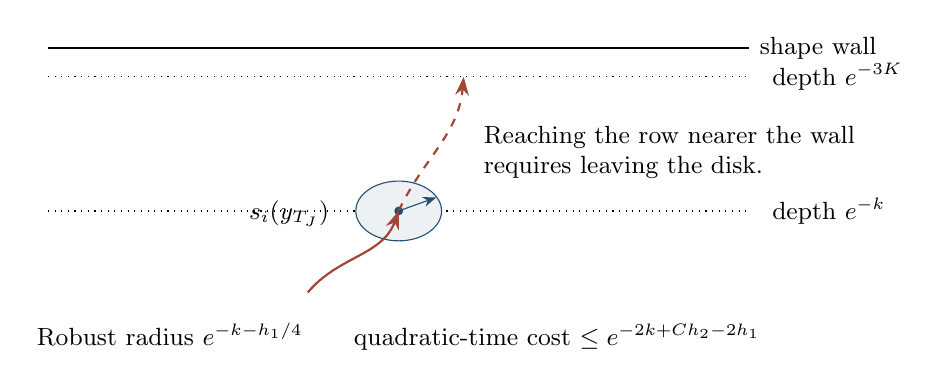
\begin{tikzpicture}[>=Stealth,x=1.65cm,y=1.15cm]
\draw[thick] (-2.7,2.4)--(2.7,2.4) node[right,font=\small] {shape wall};
\draw[dotted] (-2.7,2.08)--(2.7,2.08);
\node[font=\small,anchor=west] at (2.8,2.08) {depth $e^{-3K}$};
\draw[dotted] (-2.7,.60)--(2.7,.60);
\node[font=\small,anchor=west] at (2.8,.60) {depth $e^{-k}$};
\fill[deepblue!8] (0,.60) circle (.33);
\draw[deepblue] (0,.60) circle (.33);
\fill[deepblue] (0,.60) circle (1.6pt);
\node[font=\small,anchor=east] at (-.46,.57) {$s_i(y_{T_J})$};
\draw[->,warmred,thick] (-.7,-.3) to[out=50,in=-110] (0,.60);
\draw[->,warmred,dashed,thick] (0,.60) to[out=65,in=-95] (.5,2.08);
\node[font=\small,align=left,anchor=west] at (.58,1.25)
 {Reaching the row nearer the wall\\requires leaving the disk.};
\draw[->,deepblue] (0,.60)--(.29,.75);
\node[font=\small,align=center] at (0,-.79)
 {Robust radius $e^{-k-h_1/4}$\qquad quadratic-time cost
 $\le e^{-2k+Ch_2-2h_1}$};
\end{tikzpicture}
\caption{The last-site contradiction, drawn without metric scale.
For a fixed candidate set, \(T_J\) is the last of its capped first hits
of the tested row. The last site's robust sign suppresses its subsequent
quadratic time so strongly that disk exit has vanishing probability.
Its prescribed final history would nevertheless require such an exit.}
\label{fig:last-site}
\end{figure}


Disk exit is nevertheless compulsory on the classification event.
An actual last site has depth \(d\) at \(T_J=\sigma_i\), and
subsequently attains depth at most \(e^{-3K}\) by \(\tau_L\).
It cannot have attained that depth earlier, since that would already
have crossed the tested row.  The depth function is
\(1\)-Lipschitz, so its displacement before \(\tau_L\) is at least
\[
 d-e^{-3K}\ge d/2>r_{\mathrm{rob}}
\]
for large \(K\).  Thus it must leave the disk shown in
\Cref{fig:last-site}.  The finite union of
\eqref{sign:escape-probability} over all candidates \(J,i\) makes
this event have probability \(o(1)\), whereas
\Cref{sign:history-gap} and all the excluded failure estimates give
probability at least \(0.9-o(1)\).  This contradiction proves the
theorem.
\end{proof}

\subsection{Completion of the rigidity theorem}

\begin{proof}[Proof of \Cref{thm:main}]
The physical caustic-collar hypothesis gives an analytic boundary by
\Cref{thm:analytic}, and then the even joint parametrization and
nonzero area coefficient of \Cref{thm:joint-parametrization}.
The continuation and no-patch theorems produce the maximal shape
strip \(D_H\), with the natural-boundary conclusion of
\Cref{cor:shape-natural-boundary} when \(H<\infty\).

If the meromorphic normal \(a=e^{\ii\phi}\) has a zero or pole
inside this strip, \Cref{thm:isotropic-classification} already
identifies the boundary as an ellipse.  In the remaining case,
\Cref{thm:shape-lift} and \Cref{lem:f-zeros} give the holomorphic
shape fields and the intrinsic impact lift used above.  Constant
\(f\) gives a circle.  For nonconstant \(f\),
\Cref{thm:infinite-growth-exclusion} excludes both \(H=\infty\)
and infinite upper growth order at a finite wall.  At a finite wall,
\Cref{prop:subcritical-exclusion} excludes upper growth order below
one, and \Cref{thm:finite-superlinear-exclusion} excludes every
finite upper growth order above one.  The only remaining possibility
is a finite critical wall.  The critical bootstrap,
\Cref{thm:sequence-exclusion}, and the odd-slice construction place
it under the hypotheses of \Cref{thm:last-site}, which excludes it
as well.

Only an elliptic boundary, including a circle, remains.  Convexity
then identifies the domain with the interior of that ellipse.
After translation, it is therefore described by a positive definite
quadratic form, as asserted.
\end{proof}

\phantomsection
\addcontentsline{toc}{section}{References}
\bibliographystyle{alphaurl}
\bibliography{references/references}
\end{document}
